% Options for packages loaded elsewhere
\PassOptionsToPackage{unicode}{hyperref}
\PassOptionsToPackage{hyphens}{url}
%
\documentclass[
]{report}
\usepackage{amsmath,amssymb}
\usepackage{iftex}
\ifPDFTeX
  \usepackage[T1]{fontenc}
  \usepackage[utf8]{inputenc}
  \usepackage{textcomp} % provide euro and other symbols
\else % if luatex or xetex
  \usepackage{unicode-math} % this also loads fontspec
  \defaultfontfeatures{Scale=MatchLowercase}
  \defaultfontfeatures[\rmfamily]{Ligatures=TeX,Scale=1}
\fi
\usepackage{lmodern}
\ifPDFTeX\else
  % xetex/luatex font selection
\fi
% Use upquote if available, for straight quotes in verbatim environments
\IfFileExists{upquote.sty}{\usepackage{upquote}}{}
\IfFileExists{microtype.sty}{% use microtype if available
  \usepackage[]{microtype}
  \UseMicrotypeSet[protrusion]{basicmath} % disable protrusion for tt fonts
}{}
\makeatletter
\@ifundefined{KOMAClassName}{% if non-KOMA class
  \IfFileExists{parskip.sty}{%
    \usepackage{parskip}
  }{% else
    \setlength{\parindent}{0pt}
    \setlength{\parskip}{6pt plus 2pt minus 1pt}}
}{% if KOMA class
  \KOMAoptions{parskip=half}}
\makeatother
\usepackage{xcolor}
\usepackage{color}
\usepackage{fancyvrb}
\newcommand{\VerbBar}{|}
\newcommand{\VERB}{\Verb[commandchars=\\\{\}]}
\DefineVerbatimEnvironment{Highlighting}{Verbatim}{commandchars=\\\{\}}
% Add ',fontsize=\small' for more characters per line
\usepackage{framed}
\definecolor{shadecolor}{RGB}{248,248,248}
\newenvironment{Shaded}{\begin{snugshade}}{\end{snugshade}}
\newcommand{\AlertTok}[1]{\textcolor[rgb]{0.94,0.16,0.16}{#1}}
\newcommand{\AnnotationTok}[1]{\textcolor[rgb]{0.56,0.35,0.01}{\textbf{\textit{#1}}}}
\newcommand{\AttributeTok}[1]{\textcolor[rgb]{0.13,0.29,0.53}{#1}}
\newcommand{\BaseNTok}[1]{\textcolor[rgb]{0.00,0.00,0.81}{#1}}
\newcommand{\BuiltInTok}[1]{#1}
\newcommand{\CharTok}[1]{\textcolor[rgb]{0.31,0.60,0.02}{#1}}
\newcommand{\CommentTok}[1]{\textcolor[rgb]{0.56,0.35,0.01}{\textit{#1}}}
\newcommand{\CommentVarTok}[1]{\textcolor[rgb]{0.56,0.35,0.01}{\textbf{\textit{#1}}}}
\newcommand{\ConstantTok}[1]{\textcolor[rgb]{0.56,0.35,0.01}{#1}}
\newcommand{\ControlFlowTok}[1]{\textcolor[rgb]{0.13,0.29,0.53}{\textbf{#1}}}
\newcommand{\DataTypeTok}[1]{\textcolor[rgb]{0.13,0.29,0.53}{#1}}
\newcommand{\DecValTok}[1]{\textcolor[rgb]{0.00,0.00,0.81}{#1}}
\newcommand{\DocumentationTok}[1]{\textcolor[rgb]{0.56,0.35,0.01}{\textbf{\textit{#1}}}}
\newcommand{\ErrorTok}[1]{\textcolor[rgb]{0.64,0.00,0.00}{\textbf{#1}}}
\newcommand{\ExtensionTok}[1]{#1}
\newcommand{\FloatTok}[1]{\textcolor[rgb]{0.00,0.00,0.81}{#1}}
\newcommand{\FunctionTok}[1]{\textcolor[rgb]{0.13,0.29,0.53}{\textbf{#1}}}
\newcommand{\ImportTok}[1]{#1}
\newcommand{\InformationTok}[1]{\textcolor[rgb]{0.56,0.35,0.01}{\textbf{\textit{#1}}}}
\newcommand{\KeywordTok}[1]{\textcolor[rgb]{0.13,0.29,0.53}{\textbf{#1}}}
\newcommand{\NormalTok}[1]{#1}
\newcommand{\OperatorTok}[1]{\textcolor[rgb]{0.81,0.36,0.00}{\textbf{#1}}}
\newcommand{\OtherTok}[1]{\textcolor[rgb]{0.56,0.35,0.01}{#1}}
\newcommand{\PreprocessorTok}[1]{\textcolor[rgb]{0.56,0.35,0.01}{\textit{#1}}}
\newcommand{\RegionMarkerTok}[1]{#1}
\newcommand{\SpecialCharTok}[1]{\textcolor[rgb]{0.81,0.36,0.00}{\textbf{#1}}}
\newcommand{\SpecialStringTok}[1]{\textcolor[rgb]{0.31,0.60,0.02}{#1}}
\newcommand{\StringTok}[1]{\textcolor[rgb]{0.31,0.60,0.02}{#1}}
\newcommand{\VariableTok}[1]{\textcolor[rgb]{0.00,0.00,0.00}{#1}}
\newcommand{\VerbatimStringTok}[1]{\textcolor[rgb]{0.31,0.60,0.02}{#1}}
\newcommand{\WarningTok}[1]{\textcolor[rgb]{0.56,0.35,0.01}{\textbf{\textit{#1}}}}
\usepackage{longtable,booktabs,array}
\usepackage{calc} % for calculating minipage widths
% Correct order of tables after \paragraph or \subparagraph
\usepackage{etoolbox}
\makeatletter
\patchcmd\longtable{\par}{\if@noskipsec\mbox{}\fi\par}{}{}
\makeatother
% Allow footnotes in longtable head/foot
\IfFileExists{footnotehyper.sty}{\usepackage{footnotehyper}}{\usepackage{footnote}}
\makesavenoteenv{longtable}
\usepackage{graphicx}
\makeatletter
\def\maxwidth{\ifdim\Gin@nat@width>\linewidth\linewidth\else\Gin@nat@width\fi}
\def\maxheight{\ifdim\Gin@nat@height>\textheight\textheight\else\Gin@nat@height\fi}
\makeatother
% Scale images if necessary, so that they will not overflow the page
% margins by default, and it is still possible to overwrite the defaults
% using explicit options in \includegraphics[width, height, ...]{}
\setkeys{Gin}{width=\maxwidth,height=\maxheight,keepaspectratio}
% Set default figure placement to htbp
\makeatletter
\def\fps@figure{htbp}
\makeatother
\setlength{\emergencystretch}{3em} % prevent overfull lines
\providecommand{\tightlist}{%
  \setlength{\itemsep}{0pt}\setlength{\parskip}{0pt}}
\setcounter{secnumdepth}{5}
% definitions for citeproc citations
\NewDocumentCommand\citeproctext{}{}
\NewDocumentCommand\citeproc{mm}{%
  \begingroup\def\citeproctext{#2}\cite{#1}\endgroup}
\makeatletter
 % allow citations to break across lines
 \let\@cite@ofmt\@firstofone
 % avoid brackets around text for \cite:
 \def\@biblabel#1{}
 \def\@cite#1#2{{#1\if@tempswa , #2\fi}}
\makeatother
\newlength{\cslhangindent}
\setlength{\cslhangindent}{1.5em}
\newlength{\csllabelwidth}
\setlength{\csllabelwidth}{3em}
\newenvironment{CSLReferences}[2] % #1 hanging-indent, #2 entry-spacing
 {\begin{list}{}{%
  \setlength{\itemindent}{0pt}
  \setlength{\leftmargin}{0pt}
  \setlength{\parsep}{0pt}
  % turn on hanging indent if param 1 is 1
  \ifodd #1
   \setlength{\leftmargin}{\cslhangindent}
   \setlength{\itemindent}{-1\cslhangindent}
  \fi
  % set entry spacing
  \setlength{\itemsep}{#2\baselineskip}}}
 {\end{list}}
\usepackage{calc}
\newcommand{\CSLBlock}[1]{\hfill\break\parbox[t]{\linewidth}{\strut\ignorespaces#1\strut}}
\newcommand{\CSLLeftMargin}[1]{\parbox[t]{\csllabelwidth}{\strut#1\strut}}
\newcommand{\CSLRightInline}[1]{\parbox[t]{\linewidth - \csllabelwidth}{\strut#1\strut}}
\newcommand{\CSLIndent}[1]{\hspace{\cslhangindent}#1}
\usepackage{booktabs}
\usepackage{geometry}
\usepackage[none]{hyphenat}
\usepackage{titlesec}
\usepackage{longtable}
\usepackage{xcolor}
\usepackage{setspace}
\usepackage{pdfpages}

\pagestyle{plain}

%%%% Set margins
\setlength{\topmargin}{-1cm}
\addtolength{\evensidemargin}{-1cm}
\addtolength{\oddsidemargin}{-1cm}
\addtolength{\textheight}{3cm}
\addtolength{\textwidth}{2cm}

% Spacing for reading guides
\newcommand{\rgs}{\vspace{12pt}} % Vertical space
\newcommand{\rgi}{\hspace{24pt}}  % Indent

\newcommand\latexcode[1]{#1}

% Format chapter titles and spacing
\renewcommand*{\chaptername}{Module}

\titleformat{\chapter}[display]
{\bfseries\Large}
{\filleft\MakeUppercase{\chaptertitlename} \Huge\thechapter}
{3ex}
{\titlerule
\vspace{1.5ex}%
\filright}
[\vspace{1.5ex}%
\titlerule]
\titlespacing*{\chapter}{0pt}{-40pt}{20pt}
\ifLuaTeX
  \usepackage{selnolig}  % disable illegal ligatures
\fi
\usepackage{bookmark}
\IfFileExists{xurl.sty}{\usepackage{xurl}}{} % add URL line breaks if available
\urlstyle{same}
\hypersetup{
  hidelinks,
  pdfcreator={LaTeX via pandoc}}

\title{\textbf{STAT 216 Coursepack}\\
\strut \\
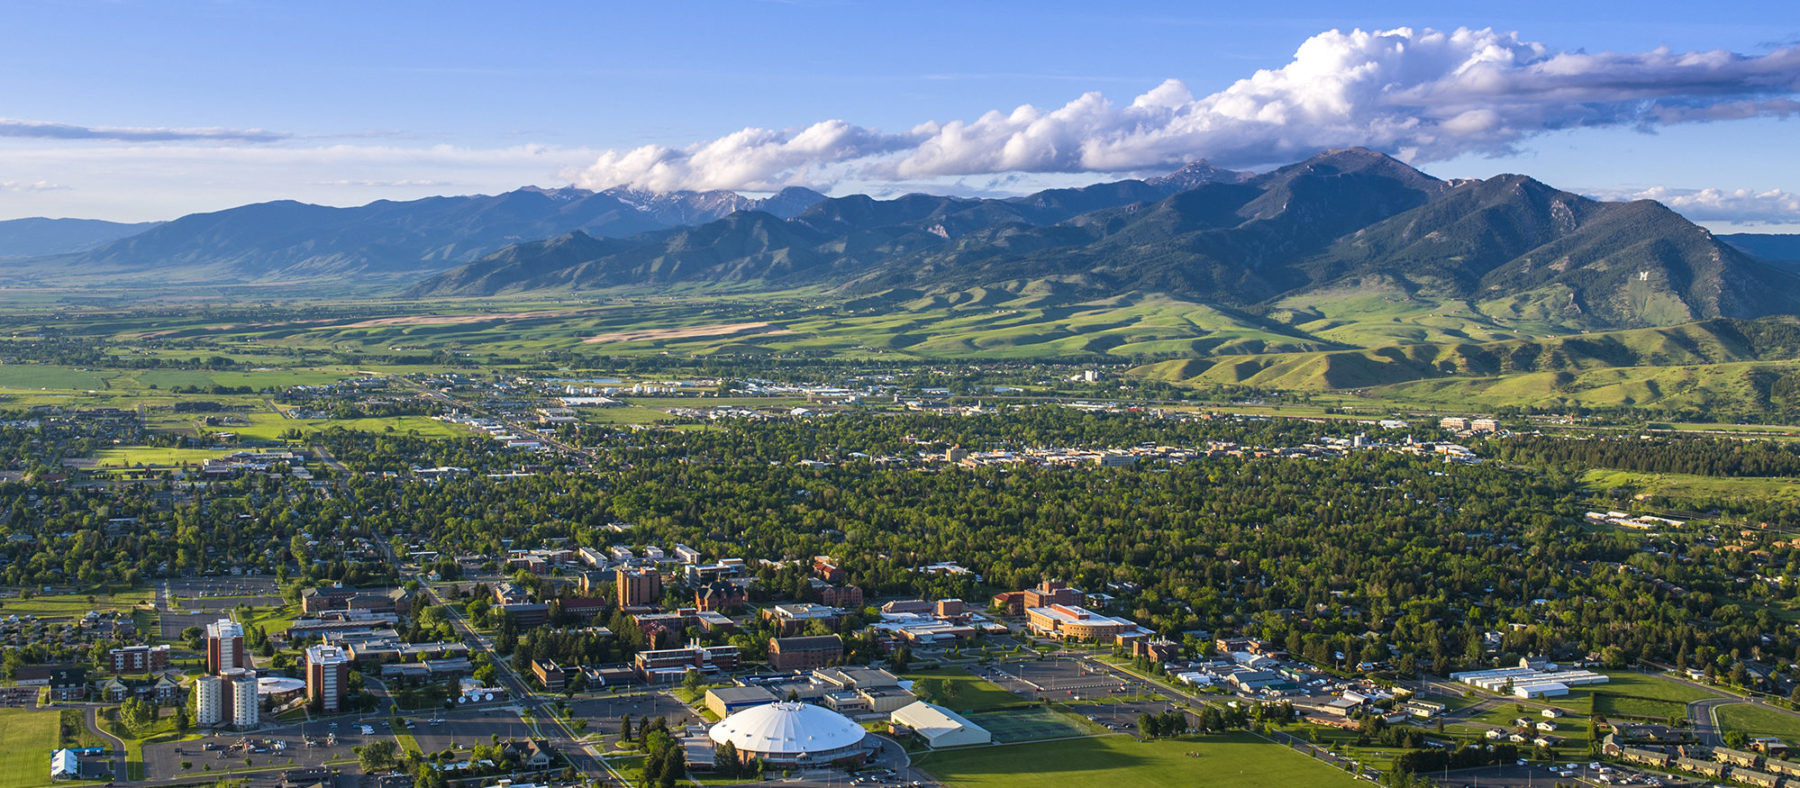
\includegraphics[width=5in,height=\textheight]{images/msu-campus.jpg}}
\usepackage{etoolbox}
\makeatletter
\providecommand{\subtitle}[1]{% add subtitle to \maketitle
  \apptocmd{\@title}{\par {\large #1 \par}}{}{}
}
\makeatother
\subtitle{Spring 2025\\
Montana State University}
\author{Melinda Yager\\
Jade Schmidt\\
Stacey Hancock}
\date{}

\begin{document}
\maketitle

\newpage
\thispagestyle{empty}

This resource was developed by Melinda Yager, Jade Schmidt, and Stacey Hancock in 2021 to accompany the online textbook: Hancock, S., Carnegie, N., Meyer, E., Schmidt, J., and Yager, M. (2021). \emph{Montana State Introductory Statistics with R}. Montana State University. \url{https://mtstateintrostats.github.io/IntroStatTextbook/}.

This resource is released under a \href{https://creativecommons.org/licenses/by-nc-sa/4.0/}{Creative Commons BY-NC-SA 4.0} license unless otherwise noted.

\setcounter{tocdepth}{1}
\addtocontents{toc}{\protect\thispagestyle{empty}}
\tableofcontents
\thispagestyle{empty}

\newpage
\setcounter{page}{1}

\chapter*{Preface}\label{preface}
\addcontentsline{toc}{chapter}{Preface}

This coursepack accompanies the textbook for STAT 216: Montana State Introductory Statistics with R, which can be found at \url{https://mtstateintrostats.github.io/IntroStatTextbook/}. The syllabus for the course (including the course calendar), data sets, and links to D2L Brightspace, Gradescope, and the MSU RStudio server can be found on the course webpage: \url{https://math.montana.edu/courses/s216/}.
Other notes and review materials are linked in D2L.

Each of the activities in this workbook is designed to target specific learning outcomes of the course, giving you practice with important statistical concepts in a group setting with instructor guidance. In addition to the in-class activities for the course, video notes are provided to aid in taking notes while you complete the required videos. Bring this workbook with you to class each class period, and take notes in the workbook as you would your own notes. A well-written completed workbook will provide an optimal study guide for exams!

All activities and labs in this coursepack will be completed during class time. Parts of each lab will be turned in on Gradescope. To aid in your understanding, read through the introduction for each activity before attending class each day.

STAT 216 is a 3-credit in-person course. In our experience, it takes six to nine hours per week outside of class to achieve a good grade in this class. By ``good'' we mean at least a C because a grade of D or below does not count toward fulfilling degree requirements. Many of you set your goals higher than just getting a C, and we fully support that. You need roughly nine hours per week to review past activities, read feedback on previous assignments, complete current assignments, and prepare for the next day's class. A typical week in the life of a STAT 216 student looks like:

\begin{itemize}
\tightlist
\item
  \emph{Prior to class meeting}:

  \begin{itemize}
  \tightlist
  \item
    Read assigned sections of the textbook, using the provided reading guides to take notes on the material.
  \item
    Watch the provided videos, taking notes in the coursepack.
  \item
    Read through the introduction to the day's in-class activity.
  \item
    Read through the week's homework assignment and note any questions you may have on the content.
  \end{itemize}
\item
  \emph{During class meeting}:

  \begin{itemize}
  \tightlist
  \item
    Work through the guided activity, in-class activity or weekly lab with your classmates and instructor, taking detailed notes on your answers to each question in the activity.
  \end{itemize}
\item
  \emph{After class meeting}:

  \begin{itemize}
  \tightlist
  \item
    Complete any parts of the activity you did not complete in class.
  \item
    Review the activity solutions in the Math and Stat Center, and take notes on key points.
  \item
    Complete any remaining assigned readings for the week.
  \item
    Complete the week's homework assignment.
  \end{itemize}
\end{itemize}

\nocite{*}

\chapter{Inference for Inference for a Paired Mean Difference}\label{inference-for-inference-for-a-paired-mean-difference}

\section{Vocabulary Review and Key Topics}\label{vocabulary-review-and-key-topics}

Review the Golden Ticket posted in the resources at the end of the coursepack for a summary of paired data. Module 11 will cover inference using both simulation and theory-based methods.

\begin{itemize}
\item
  The \textbf{summary measure} for one quantitative variable is the \textbf{mean difference}
\item
  Paired differences are treated as a single mean. Review the summary of Module 6 for interpretations of other summary measures from quantitative data and for the type of plots used.
\item
  R code to find the summary statistics for a paired differences
\end{itemize}

\subsection*{Simulation Hypothesis Testing}\label{simulation-hypothesis-testing}
\addcontentsline{toc}{subsection}{Simulation Hypothesis Testing}

Hypotheses:

\[H_0: \mu_d = 0\]
\[H_A: \mu_d\left\{
\begin{array}{ll}
< \\
\ne \\
< \\
\end{array}
\right\}
0 \]

\begin{itemize}
\tightlist
\item
  R code to use for \textbf{simulation methods} for one paired data to find the p-value, \texttt{paired\_test}, is shown below. Review the comments (instructions after the \#) to see what each should be entered for each line of code.
\end{itemize}

\begin{Shaded}
\begin{Highlighting}[]
\FunctionTok{paired\_test}\NormalTok{(}\AttributeTok{data =}\NormalTok{ object}\SpecialCharTok{$}\NormalTok{differences,   }\CommentTok{\# Vector of differences }
                                         \CommentTok{\# or data set with column for each group}
            \AttributeTok{shift =}\NormalTok{ xx,   }\CommentTok{\# Shift needed for bootstrap hypothesis test}
            \AttributeTok{as\_extreme\_as =}\NormalTok{ xx,  }\CommentTok{\# Observed statistic}
            \AttributeTok{direction =} \StringTok{"xx"}\NormalTok{,  }\CommentTok{\# Direction of alternative}
            \AttributeTok{number\_repetitions =} \DecValTok{10000}\NormalTok{,  }\CommentTok{\# Number of simulated samples for null distribution}
            \AttributeTok{which\_first =} \DecValTok{1}\NormalTok{)  }\CommentTok{\# Not needed when using calculated differences}
\end{Highlighting}
\end{Shaded}

\subsection*{Simulation Confidence Interval}\label{simulation-confidence-interval}
\addcontentsline{toc}{subsection}{Simulation Confidence Interval}

\begin{itemize}
\tightlist
\item
  R code to find the simulation confidence interval using the \texttt{paired\_bootstrap\_CI} function from the \texttt{catstats} package.
\end{itemize}

\begin{Shaded}
\begin{Highlighting}[]
\FunctionTok{paired\_bootstrap\_CI}\NormalTok{(}\AttributeTok{data =}\NormalTok{ object}\SpecialCharTok{$}\NormalTok{differences, }\CommentTok{\# Enter vector of differences}
                    \AttributeTok{number\_repetitions =} \DecValTok{10000}\NormalTok{, }\CommentTok{\# Number of bootstrap samples for CI}
                    \AttributeTok{confidence\_level =}\NormalTok{ xx,  }\CommentTok{\# Confidence level in decimal form}
                    \AttributeTok{which\_first =} \DecValTok{1}\NormalTok{)  }\CommentTok{\# Not needed when entering vector of differences}
\end{Highlighting}
\end{Shaded}

\begin{itemize}
\tightlist
\item
  The interpretation of the confidence interval is very similar for that of a single mean. Just make sure to add the order of subtraction for the differences.
\end{itemize}

\subsection*{Theory-based Methods}\label{theory-based-methods}
\addcontentsline{toc}{subsection}{Theory-based Methods}

\begin{itemize}
\item
  \textbf{Conditions for the sampling distribution of \(\bar{x}_d\) to follow an approximate normal distribution}:

  \begin{itemize}
  \item
    \textbf{Independence}: The sample's observations are independent, e.g., are from a simple random sample. (\emph{Remember}: This also must be true to use simulation methods!)
  \item
    \textbf{Large enough sample size: Normality Condition}: The sample observations come from a normally distributed population. To check use the the following rules of thumb:

    \begin{itemize}
    \item
      \(n < 30\): The distribution of the sample must be approximately normal with no outliers
    \item
      \(30 \ge n < 100\): We can relax the condition a little; the distribution of the sample must have no extreme outliers or skewness
    \item
      \(n > 100\): Can assume the sampling distribution of \(\bar{x}\) is nearly normal, even if the underlying distribuion of individual observationals is not
    \end{itemize}
  \end{itemize}
\item
  \textbf{t-distribution}: a theoretical distribution that is symmetric with a given degrees of freedom (\(n-1\))

  \begin{itemize}
  \tightlist
  \item
    \(t_{n-1}\)
  \end{itemize}
\item
  Calculation of standard error:
\end{itemize}

\[SE(\bar{x}_1 - \bar{x}_2) = \sqrt{\frac{{s_1}^2}{n_1}+\frac{{s_2}^2}{n_2}}\]

\begin{itemize}
\tightlist
\item
  Calculation of the standardized difference in sample mean:
\end{itemize}

\[t = \frac{\bar{x}_1-\bar{x}_2-0}{SE(\bar{x}_1 - \bar{x}_2)}\]

\begin{itemize}
\tightlist
\item
  Calculation of the confidence interval for a difference in sample means
\end{itemize}

\[\bar{x}_1-\bar{x}_2\pm t^*\times SE(\bar{x}_1-\bar{x}_2)\]
\newpage

\section{Video Notes: Inference for Paired Data}\label{video-notes-inference-for-paired-data}

Read Chapters 17 and 18 in the course textbook. Use the following videos to complete the video notes for Module 9.

\subsection{Course Videos}\label{course-videos}

\begin{itemize}
\item
  PairedData
\item
  18.1and18.2
\item
  18.3
\end{itemize}

\setstretch{1}

\subsection*{Single categorical, single quantitative variables Video Paired\_Data}\label{single-categorical-single-quantitative-variables-video-paired_data}
\addcontentsline{toc}{subsection}{Single categorical, single quantitative variables Video Paired\_Data}

\begin{itemize}
\tightlist
\item
  In this module, we will study inference for a \_\_\_\_\_\_\_\_\_\_\_\_\_\_\_\_\_\_\_\_\_\_ explanatory variable and a \_\_\_\_\_\_\_\_\_\_\_\_\_\_\_\_\_\_\_\_\_\_\_\_\_ response variable where the two groups are \_\_\_\_\_\_\_\_\_\_\_\_\_\_\_\_\_\_\_\_\_\_\_\_\_\_\_\_.
\end{itemize}

\subsection*{Paired vs.~Independent Samples}\label{paired-vs.-independent-samples}
\addcontentsline{toc}{subsection}{Paired vs.~Independent Samples}

Two groups are paired if an observational unit in one group is connected to an observational unit in another group

\rgi Data are paired if the samples are \_\_\_\_\_\_\_\_\_\_\_\_\_\_\_\_\_\_\_

Examples:

\begin{itemize}
\item
  Change in test score from pre and post test
\item
  Weight of college students before and after 1st year
\item
  Change in blood pressure
\end{itemize}

\begin{figure}

{\centering 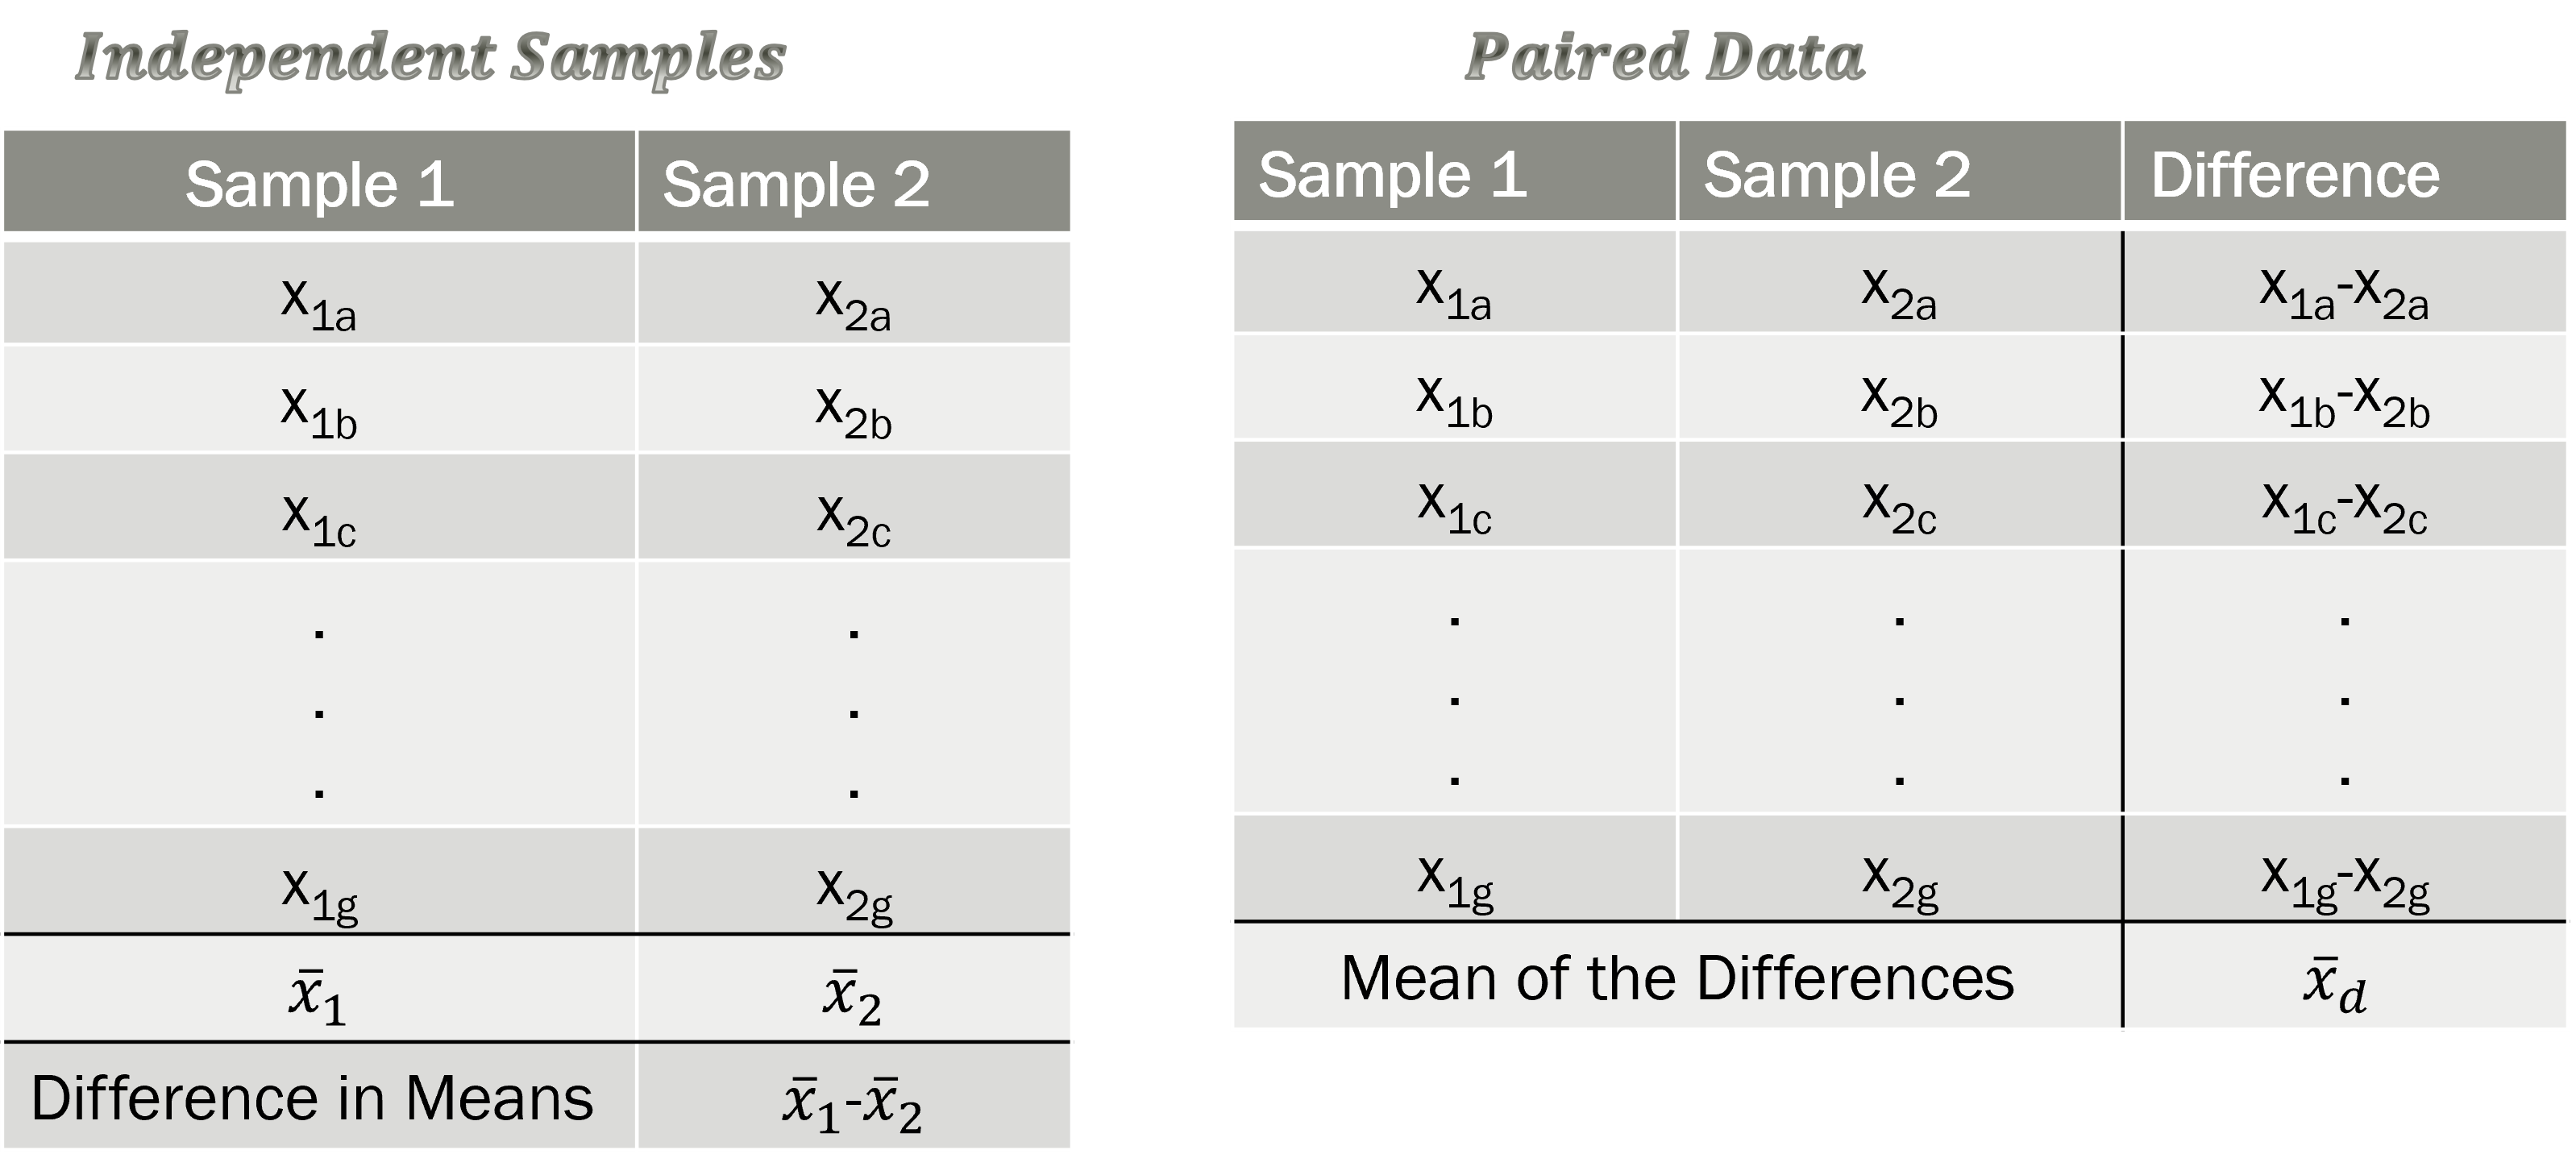
\includegraphics[width=0.6\linewidth]{images/paired_independent} 

}

\caption{Illustration of Independent vs. Paired Samples}\label{fig:pairedindependent}
\end{figure}

Example 1: Three hundred registered voters were selected at random to participate in a study on attitudes about how well the president is performing. They were each asked to answer a short multiple-choice questionnaire and then they watched a 20-minute video that presented information about the job description of the president. After watching the video, the same 300 selected voters were asked to answer a follow-up multiple-choice questionnaire.

\begin{itemize}
\tightlist
\item
  Is this an example of a paired samples or independent samples study?
\end{itemize}

\vspace{0.3in}

\newpage

Example 2: Thirty dogs were selected at random from those residing at the humane society last month. The 30 dogs were split at random into two groups. The first group of 15 dogs was trained to perform a certain task using a reward method. The second group of 15 dogs was trained to perform the same task using a reward-punishment method.

\begin{itemize}
\tightlist
\item
  Is this an example of a paired samples or independent samples study?
\end{itemize}

\vspace{0.3in}

Example 3: Fifty skiers volunteered to study how different waxes impacted their downhill race times. The participants were split into groups of two based on similar race times from the previous race. One of the two then had their skis treated with Wax A while the other was treated with Wax B. The downhill ski race times were then measured for each of the 25 volunteers who used Wax A as well as for each of the 25 volunteers who used Wax B.

\begin{itemize}
\tightlist
\item
  Is this an example of a paired samples or independent samples study?
\end{itemize}

\vspace{0.3in}

Example: Is there a difference in heights between husbands and wives? The heights were measured on the husband and wife in a random sample of 199 married couples from Great Britain ({``Great Britain Married Couples: Great Britain Office of Population Census and Surveys,''} n.d.).

For a paired experiment, we look at the difference between responses for each unit (pair), rather than just the average difference between treatment groups

\begin{Shaded}
\begin{Highlighting}[]
\NormalTok{hw }\OtherTok{\textless{}{-}}\FunctionTok{read.csv}\NormalTok{(}\StringTok{"data/husbands\_wives\_ht.csv"}\NormalTok{)}
\FunctionTok{paired\_observed\_plot}\NormalTok{(hw)}
\end{Highlighting}
\end{Shaded}

\begin{center}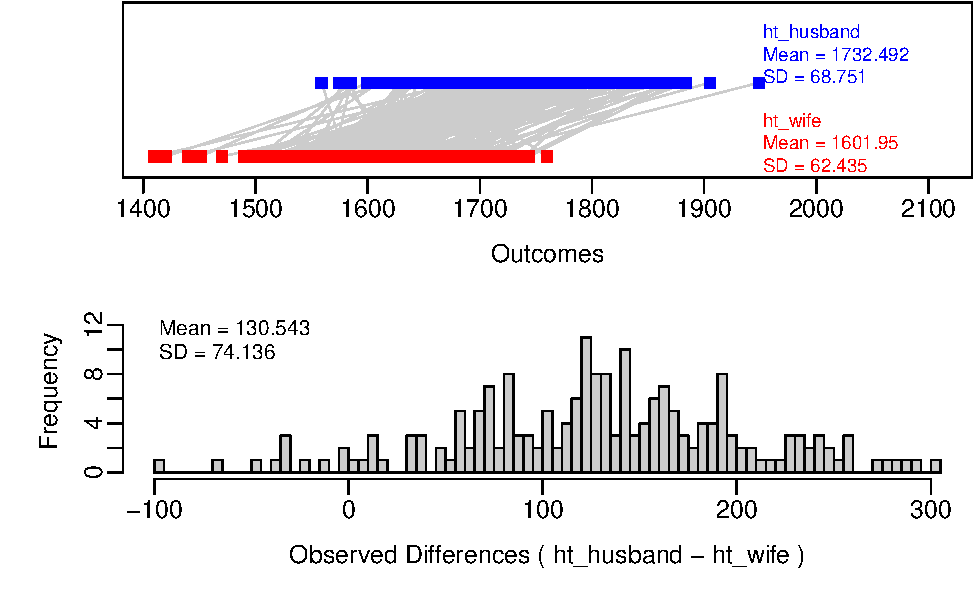
\includegraphics[width=0.7\linewidth]{11-VN11-paired_files/figure-latex/unnamed-chunk-1-1} \end{center}

\begin{Shaded}
\begin{Highlighting}[]
\NormalTok{hw\_diff }\SpecialCharTok{\%\textgreater{}\%}
    \FunctionTok{summarise}\NormalTok{(}\FunctionTok{fav\_stats}\NormalTok{(ht\_diff))}
\end{Highlighting}
\end{Shaded}

\begin{verbatim}
#>   min   Q1 median  Q3 max     mean       sd   n missing
#> 1 -96 83.5    131 179 303 130.5427 74.13608 199       0
\end{verbatim}

\setstretch{1.5}

\begin{itemize}
\tightlist
\item
  The summary measure for paired data is the \_\_\_\_\_\_\_\_\_\_\_\_\_\_\_\_\_\_\_\_\_\_\_.
\end{itemize}

\newpage

\begin{itemize}
\tightlist
\item
  Mean difference: the average \_\_\_\_\_\_\_\_\_\_\_\_\_\_\_ in the \_\_\_\_\_\_\_\_\_\_\_\_\_\_\_\_\_
  variable outcomes for observational units between \_\_\_\_\_\_\_\_\_\_\_\_\_\_\_\_\_\_\_\_ variable groups
\end{itemize}

\setstretch{1}

Notation for the Paired differences

\begin{itemize}
\item
  Population mean of the differences:
\item
  Population standard deviation of the differences:
\item
  Sample mean of the differences:
\item
  Sample standard deviation of the differences:
\end{itemize}

Conditions for inference for paired data:

\begin{itemize}
\tightlist
\item
  Independence:
\end{itemize}

\vspace{0.5in}

Is the independence condition met for the height study?

\vspace{0.5in}

\subsection*{Hypothesis testing}\label{hypothesis-testing}
\addcontentsline{toc}{subsection}{Hypothesis testing}

Null hypothesis assumes ``no effect'', ``no difference'', ``nothing interesting happening'', etc.

\begin{itemize}
\item
  Treat the differences like a single mean
\item
  Always of form: ``parameter'' = null value
\end{itemize}

\(H_0:\)

\vspace{0.2in}

\(H_A:\)

\vspace{0.2in}

\begin{itemize}
\tightlist
\item
  Research question determines the direction of the alternative hypothesis.
\end{itemize}

Write the null and alternative for the height study:

In notation:

\(H_0:\)

\vspace{0.2in}

\(H_A:\)

\vspace{0.2in}

\subsubsection*{Simulation-based method}\label{simulation-based-method}
\addcontentsline{toc}{subsubsection}{Simulation-based method}

\begin{itemize}
\item
  Simulate many samples assuming \(H_0: \mu_d = 0\)

  \begin{itemize}
  \item
    Shift the data by the difference between \(\mu_0\) and \(\bar{x}_d\)
  \item
    Sample with replacement \(n\) times from the shifted data
  \item
    Plot the simulated shifted sample mean from each simulation
  \item
    Repeat 1000 times (simulations) to create the null distribution
  \item
    Find the proportion of simulations at least as extreme as \(\bar{x}_d\)
  \end{itemize}
\end{itemize}

Reminder of summary statistics:

\begin{Shaded}
\begin{Highlighting}[]
\NormalTok{hw\_diff }\SpecialCharTok{\%\textgreater{}\%}
    \FunctionTok{summarise}\NormalTok{(}\FunctionTok{fav\_stats}\NormalTok{(ht\_diff))}
\end{Highlighting}
\end{Shaded}

\begin{verbatim}
#>   min   Q1 median  Q3 max     mean       sd   n missing
#> 1 -96 83.5    131 179 303 130.5427 74.13608 199       0
\end{verbatim}

Find the difference:

\(\mu_0 - \bar{x}_d =\)

Simulated null distribution:

\begin{Shaded}
\begin{Highlighting}[]
\FunctionTok{set.seed}\NormalTok{(}\DecValTok{216}\NormalTok{)}
\FunctionTok{paired\_test}\NormalTok{(}\AttributeTok{data =}\NormalTok{ hw\_diff}\SpecialCharTok{$}\NormalTok{ht\_diff,   }\CommentTok{\# Vector of differences }
                                         \CommentTok{\# or data set with column for each group}
            \AttributeTok{shift =} \SpecialCharTok{{-}}\FloatTok{130.543}\NormalTok{,   }\CommentTok{\# Shift needed for bootstrap hypothesis test}
            \AttributeTok{as\_extreme\_as =} \FloatTok{130.543}\NormalTok{,  }\CommentTok{\# Observed statistic}
            \AttributeTok{direction =} \StringTok{"two{-}sided"}\NormalTok{,  }\CommentTok{\# Direction of alternative}
            \AttributeTok{number\_repetitions =} \DecValTok{10000}\NormalTok{,  }\CommentTok{\# Number of simulated samples for null distribution}
            \AttributeTok{which\_first =} \DecValTok{1}\NormalTok{)  }\CommentTok{\# Not needed when using calculated differences}
\end{Highlighting}
\end{Shaded}

\begin{center}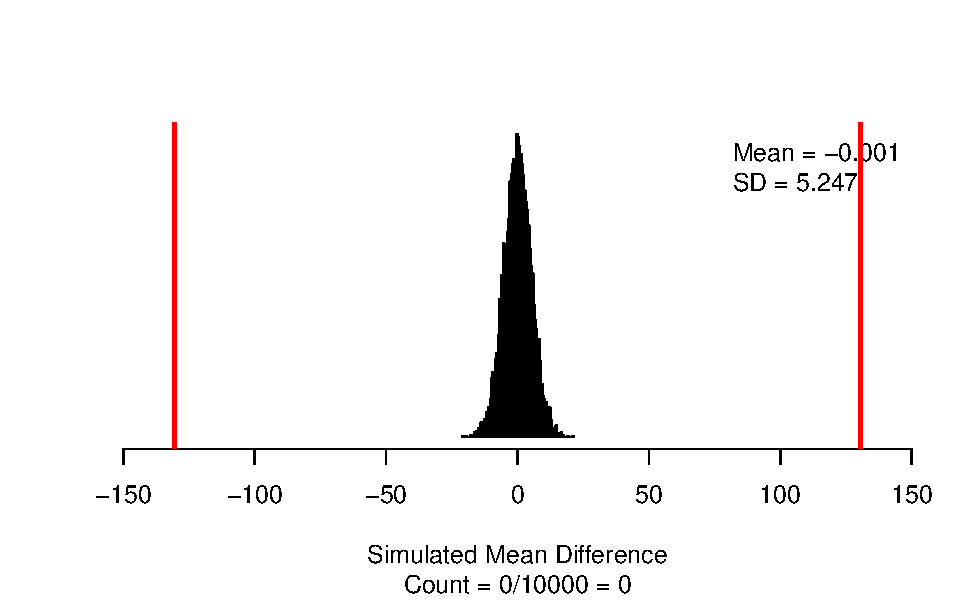
\includegraphics[width=0.7\linewidth]{11-VN11-paired_files/figure-latex/unnamed-chunk-5-1} \end{center}

Interpret the p-value:

\begin{itemize}
\item
  Statement about probability or proportion of samples
\item
  Statistic (summary measure and value)
\item
  Direction of the alternative
\item
  Null hypothesis (in context)
\end{itemize}

\vspace{0.8in}

\newpage

Conclusion:

\begin{itemize}
\item
  Amount of evidence
\item
  Parameter of interest
\item
  Direction of the alternative hypothesis
\end{itemize}

\vspace{0.8in}

\subsection*{Confidence interval}\label{confidence-interval}
\addcontentsline{toc}{subsection}{Confidence interval}

\subsubsection*{Simulation-based method}\label{simulation-based-method-1}
\addcontentsline{toc}{subsubsection}{Simulation-based method}

\begin{itemize}
\item
  Label cards with the values (differences) from the data set
\item
  Sample with replacement (bootstrap) from the original sample \(n\) times
\item
  Plot the simulated sample mean on the bootstrap distribution
\item
  Repeat at least 1000 times (simulations)
\item
  Find the cut-offs for the middle X\% (confidence level) in a bootstrap distribution.

  \begin{itemize}
  \tightlist
  \item
    i.e., 95\% CI = (2.5th percentile, 97.5th percentile)
  \end{itemize}
\end{itemize}

Simulated bootstrap distribution:

\begin{Shaded}
\begin{Highlighting}[]
\FunctionTok{set.seed}\NormalTok{(}\DecValTok{216}\NormalTok{)}
\FunctionTok{paired\_bootstrap\_CI}\NormalTok{(}\AttributeTok{data =}\NormalTok{ hw\_diff}\SpecialCharTok{$}\NormalTok{ht\_diff, }\CommentTok{\# Enter vector of differences}
            \AttributeTok{number\_repetitions =} \DecValTok{10000}\NormalTok{, }\CommentTok{\# Number of bootstrap samples for CI}
            \AttributeTok{confidence\_level =} \FloatTok{0.95}\NormalTok{,  }\CommentTok{\# Confidence level in decimal form}
            \AttributeTok{which\_first =} \DecValTok{1}\NormalTok{)  }\CommentTok{\# Not needed when entering vector of differences}
\end{Highlighting}
\end{Shaded}

\begin{center}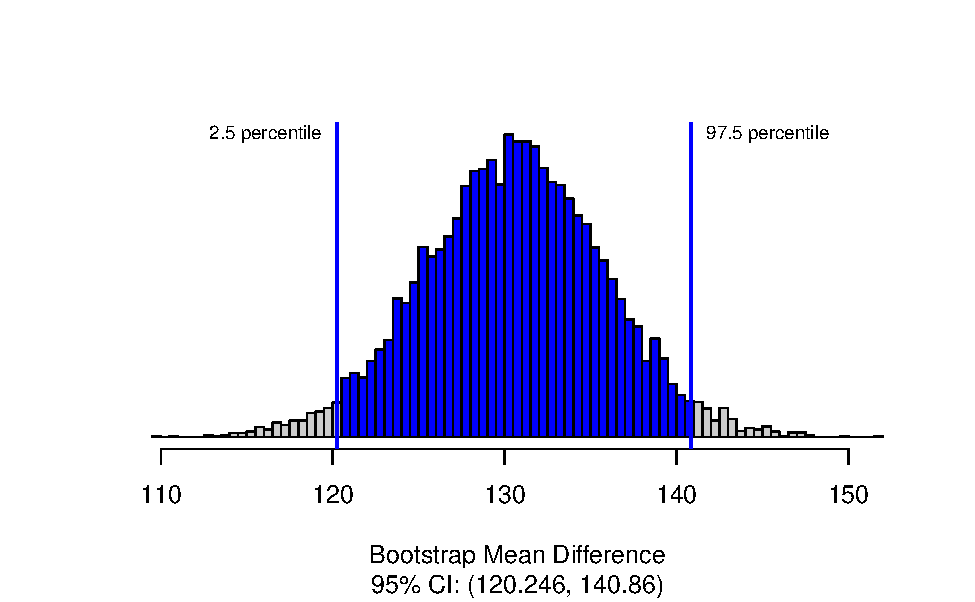
\includegraphics[width=0.7\linewidth]{11-VN11-paired_files/figure-latex/unnamed-chunk-6-1} \end{center}

\newpage

Interpret the 99\% confidence interval:

\begin{itemize}
\item
  How confident you are (e.g., 90\%, 95\%, 98\%, 99\%)
\item
  Parameter of interest
\item
  Calculated interval
\item
  Order of subtraction when comparing two groups
\end{itemize}

\vspace{0.8in}

\subsubsection*{Theory-based method - Video 18.3}\label{theory-based-method---video-18.3}
\addcontentsline{toc}{subsubsection}{Theory-based method - Video 18.3}

\subsubsection*{t-distribution}\label{t-distribution}
\addcontentsline{toc}{subsubsection}{t-distribution}

In the theoretical approach, we use the CLT to tell us that the distribution of sample means will be approximately normal, centered at the assumed true mean under \(H_0\) and with standard deviation \(\frac{\sigma}{\sqrt{n}}\).

\[\bar{x} \sim N(\mu_0, \frac{\sigma_d}{\sqrt{n}})\]
\setstretch{1.5}

\begin{itemize}
\item
  Estimate the population standard deviation, \(\sigma_d\), with the
  \_\_\_\_\_\_\_\_\_\_\_\_\_\_\_\_\_\_\_\_\_\_\_\_\_\_\_ standard deviation, \_\_\_\_\_\_\_\_.
\item
  For a single quantitative variable we use the \_\_\_\_ - distribution
  with \_\_\_\_\_\_\_\_\_\_\_\_\_\_\_
  degrees of freedom to approximate the sampling distribution.
\end{itemize}

\setstretch{1}

Conditions for inference using theory-based methods for paired data (categorical explanatory and quantitative response):

\begin{itemize}
\item
  Independence: (same as for simulation); the difference in outcome for one observational unit will not influence another observation.
\item
  Large enough sample size:

  \begin{itemize}
  \tightlist
  \item
    Normality: The data should be approximately normal or the sample size should be large.
  \end{itemize}
\end{itemize}

\rgi \rgi \(n < 30\):

\vspace{0.2in}

\rgi \rgi \(30 \leq n < 100\):

\vspace{0.2in}

\rgi \rgi \(n \geq 100\):

\vspace{0.2in}

Theory-based Hypothesis Test:

\begin{itemize}
\item
  Calculate the standardized statistic
\item
  Find the area under the t-distribution with \(n - 1\) df at least as extreme as the standardized statistic
\end{itemize}

Equation for the standard error for the sample mean difference:

\vspace{0.5in}

Equation for the standardized sample mean difference:

\vspace{0.5in}

Reminder of summary statistics for height data:

\begin{Shaded}
\begin{Highlighting}[]
\NormalTok{hw\_diff }\SpecialCharTok{\%\textgreater{}\%}
    \FunctionTok{summarise}\NormalTok{(}\FunctionTok{fav\_stats}\NormalTok{(ht\_diff))}
\end{Highlighting}
\end{Shaded}

\begin{verbatim}
#>   min   Q1 median  Q3 max     mean       sd   n missing
#> 1 -96 83.5    131 179 303 130.5427 74.13608 199       0
\end{verbatim}

Calculate the standardized sample mean difference in height:

\begin{itemize}
\tightlist
\item
  1st calculate the standard error of the sample mean difference
\end{itemize}

\vspace{0.5in}

\begin{itemize}
\tightlist
\item
  Then calculate the T score
\end{itemize}

\vspace{0.5in}

What theoretical distribution should we use to find the p-value using the value of the standardized statistic?

\vspace{0.3in}

\begin{center}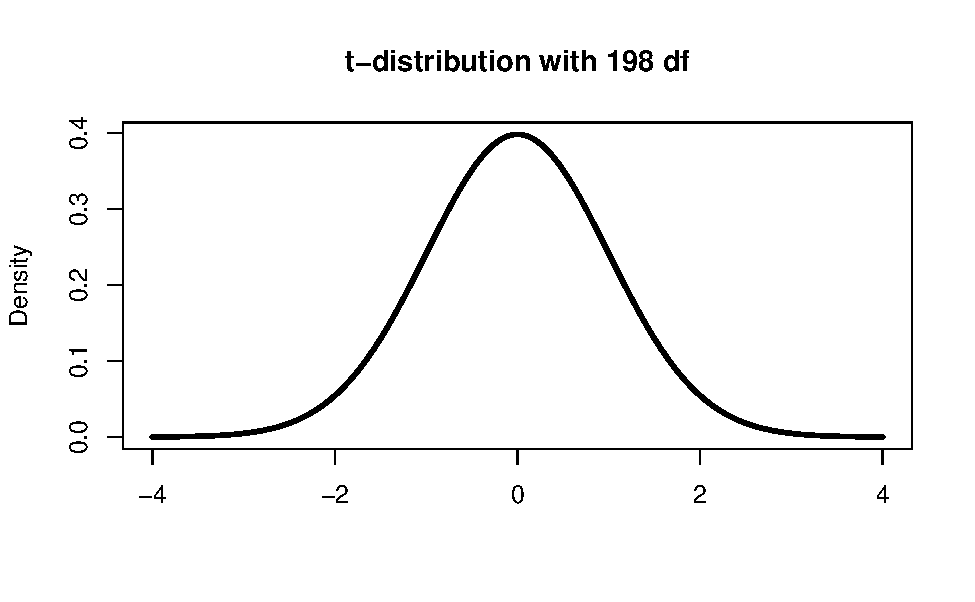
\includegraphics[width=0.7\linewidth]{11-VN11-paired_files/figure-latex/pvalueheight-1} \end{center}

To find the p-value:

\begin{Shaded}
\begin{Highlighting}[]
\FunctionTok{pt}\NormalTok{(}\FloatTok{24.84}\NormalTok{, }\AttributeTok{df =} \DecValTok{198}\NormalTok{, }\AttributeTok{lower.tail=}\ConstantTok{FALSE}\NormalTok{)}\SpecialCharTok{*}\DecValTok{2}
\end{Highlighting}
\end{Shaded}

\begin{verbatim}
#> [1] 9.477617e-63
\end{verbatim}

Theory-based Confidence Interval:

\rgi \(\text{statistic} \pm \text{margin of error}\)

\vspace{0.5in}

The \(t^*\) multiplier is the value at the given percentile of the t-distribution with \(n - 1\) degrees of freedom.

For the height data, we will use a t-distribution with \_\_\_\_\_\_\_\_\_ df.

\begin{center}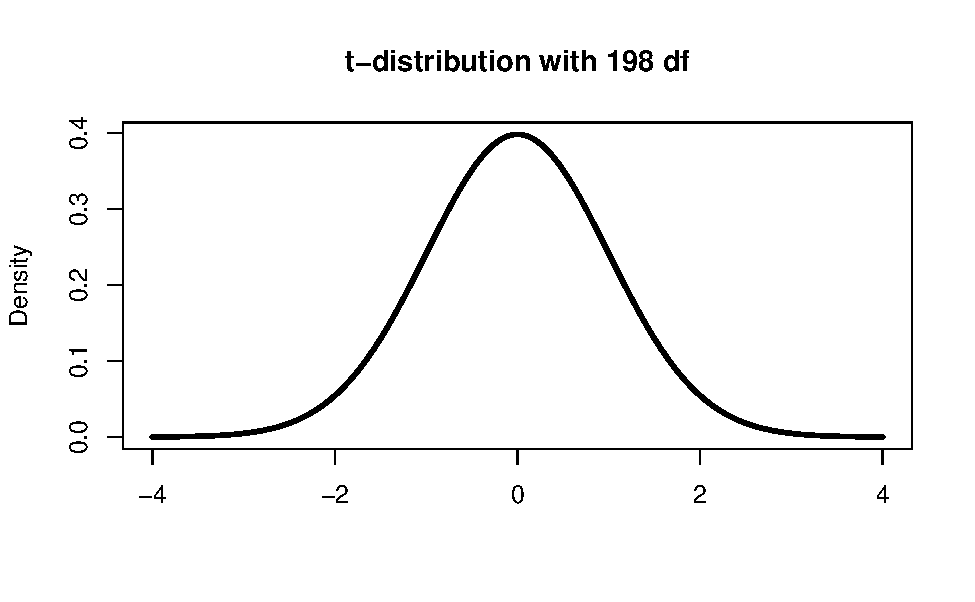
\includegraphics[width=0.7\linewidth]{11-VN11-paired_files/figure-latex/tstar-1} \end{center}

To find the \(t^*\) multiplier for a 99\% confidence interval:

\begin{Shaded}
\begin{Highlighting}[]
\FunctionTok{qt}\NormalTok{(}\FloatTok{0.975}\NormalTok{, }\AttributeTok{df=}\DecValTok{198}\NormalTok{, }\AttributeTok{lower.tail =} \ConstantTok{TRUE}\NormalTok{)}
\end{Highlighting}
\end{Shaded}

\begin{verbatim}
#> [1] 1.972017
\end{verbatim}

Calculate the margin of error:
\vspace{0.4in}

Calculate the theory-based confidence interval.
\vspace{0.5in}

\subsection{Concept Check}\label{concept-check}

Be prepared for group discussion in the next class. One member from the table should write the answers to the following on the whiteboard.

\begin{enumerate}
\def\labelenumi{\arabic{enumi}.}
\tightlist
\item
  What theoretical distribution is used to approximate paired quantitative data?
\end{enumerate}

\vspace{0.2in}

\begin{enumerate}
\def\labelenumi{\arabic{enumi}.}
\setcounter{enumi}{1}
\tightlist
\item
  What is the difference between a paired and independent study design?
\end{enumerate}

\vspace{1in}

\newpage

\section{Activity 21: Paired vs.~Independent Samples}\label{activity-21-paired-vs.-independent-samples}

\setstretch{1}

\subsection{Learning outcomes}\label{learning-outcomes}

\begin{itemize}
\item
  Determine if a data set is paired or two independent samples
\item
  Identify and create appropriate summary statistics and plots
  given a data set or research question for quantitative data.
\item
  Interpret the following summary statistics in context:
  median, lower quartile, upper quartile,
  standard deviation, interquartile range.
\end{itemize}

\subsection{Terminology review}\label{terminology-review}

In today's activity, we will review summary measures and plots for paired data. Some terms covered in this activity are:

\begin{itemize}
\item
  Mean difference
\item
\end{itemize}

To review these concepts, see Chapter 5 and 18 in the textbook.

\subsection{Paired vs.~Independent Samples}\label{paired-vs.-independent-samples-1}

For each of the following scenarios, determine whether the samples are paired or independent.

\begin{enumerate}
\def\labelenumi{\arabic{enumi}.}
\item
  Researchers interested in studying the effect of a medical treatment on insulin rate measured insulin rates of 30 patients before and after the medical treatment.
  \vspace{0.3in}
\item
  A university is planning to bring emotional support animals to campus during finals week and wants to determine which type of animals are more effective at calming students. Anxiety levels will be measured before and after each student interacts with either a dog or a cat. The university will then compare change in anxiety levels between the `dog' people and the `cat' people.
  \vspace{0.3in}
\item
  An industry leader is investigating a possible wage gap between male and non-male employees. Twenty companies within the industry are randomly selected and the average salary for all males and non-males in mid-management positions is recorded for each company.
  \vspace{0.3in}
\end{enumerate}

\subsection{Take-home messages}\label{take-home-messages}

\begin{enumerate}
\def\labelenumi{\arabic{enumi}.}
\item
  Histograms, box plots, and dot plots can all be used to graphically display a single quantitative variable.
\item
  The box plot is created using the five number summary: minimum value, quartile 1, median, quartile 3, and maximum value. Values in the data set that are less than \(\text{Q}_1 - 1.5\times \text{IQR}\) and greater than \(\text{Q}_3 + 1.5\times \text{IQR}\) are considered outliers and are graphically represented by a dot outside of the whiskers on the box plot.
\item
  Data should be summarized numerically and displayed graphically to give us information about the study.
\item
  When comparing distributions of quantitative variables we look at the shape, center, spread, and for outliers. There are two measures of center: mean and the median and two measures of spread: standard deviation and the interquartile range, IQR = Q3 \(-\) Q1.
\end{enumerate}

\subsection{Additional notes}\label{additional-notes}

Use this space to summarize your thoughts and take additional notes on today's activity and material covered.

\newpage

\section{Activity 22: Snakes}\label{activity-22-snakes}

\setstretch{1}

\subsection{Learning outcomes}\label{learning-outcomes-1}

\begin{itemize}
\item
  Given a research question involving paired differences, construct the null and alternative hypotheses
  in words and using appropriate statistical symbols.
\item
  Describe and perform a simulation-based hypothesis test for a paired mean difference.
\item
  Interpret and evaluate a p-value for a simulation-based hypothesis test for a paired mean difference.
\item
  Use bootstrapping to find a confidence interval for a paired mean difference.
\item
  Interpret a confidence interval for a paired mean difference.
\item
  Use a confidence interval to determine the conclusion of a hypothesis test.
\end{itemize}

\subsection{Terminology review}\label{terminology-review-1}

In today's activity, we will analyze paired quantitative data using simulation-based methods. Some terms covered in this activity are:

\begin{itemize}
\item
  Mean difference
\item
  Paired data
\item
  Independent groups
\item
  Shifted bootstrap (null) distribution
\end{itemize}

To review these concepts, see Section 18 in the textbook.

\subsection{Snake mazes}\label{snake-mazes}

``Sidewinding'' refers to a method of locomotion used by snakes to travel over slippery or loose terrain, such as sand. This manner of movement is a form of lateral undulation, in which an animal uses wave-like movement patterns to propel themselves forward. The desert horned viper is one of a handful of snake species that primarily uses sidewinding. As part of a recent study (Subach 2022), researchers exploring foraging behaviors of these vipers in the Sahara and western Negev deserts captured 27 unique vipers with the goal of examining how environment complexity affected movement. Each snake was placed in a circular ``maze'' of 1045 poles stuck into a sand dune (meant to simulate a dense-vegetation area). The snake was timed to see how long it took to get out of the maze. Researchers also measured how far the snake had ``traveled'' within the maze by examining the tracks left in the sand. Once the snake had completed the maze, it was allowed to travel in an open area for the same length of time as it spent in the maze; distance was again measured by the tracks in the sand. Is there evidence the distance traveled (in meters) by snakes is less in areas of dense vegetation than in open spaces, on average? Use circular maze - open area as the order of subtraction.

\begin{itemize}
\item
  Download the R script file and csv file from D2L and upload both to the RStudio server
\item
  Open the R script file and enter the name of the dataset for datasetname.csv
\item
  Highlight and run lines 1 - 7
\end{itemize}

\begin{Shaded}
\begin{Highlighting}[]
\NormalTok{snakes }\OtherTok{\textless{}{-}} \FunctionTok{read\_csv}\NormalTok{(}\StringTok{"datasetname.csv"}\NormalTok{)}
\FunctionTok{paired\_observed\_plot}\NormalTok{(snakes)}
\end{Highlighting}
\end{Shaded}

To find the difference in distance traveled in the circular maze vs in open spaces for each snake we will create the variable differences.

\begin{itemize}
\item
  Enter \texttt{DistanceMaze} for measurement\_1 and \texttt{DistanceOpen} for measurement\_2 in line 14
\item
  Highlight and run 12--22
\end{itemize}

\begin{Shaded}
\begin{Highlighting}[]
\NormalTok{snakes\_diff }\OtherTok{\textless{}{-}}\NormalTok{ snakes }\SpecialCharTok{\%\textgreater{}\%} 
  \FunctionTok{mutate}\NormalTok{(}\AttributeTok{differences =}\NormalTok{ measurement\_1 }\SpecialCharTok{{-}}\NormalTok{ measurement\_2)}
\NormalTok{snakes\_diff }\SpecialCharTok{\%\textgreater{}\%} 
    \FunctionTok{summarise}\NormalTok{(}\FunctionTok{favstats}\NormalTok{(differences))}

\NormalTok{snakes\_diff }\SpecialCharTok{\%\textgreater{}\%} 
    \FunctionTok{ggplot}\NormalTok{(}\FunctionTok{aes}\NormalTok{(}\AttributeTok{x =}\NormalTok{ differences)) }\SpecialCharTok{+}
    \FunctionTok{geom\_boxplot}\NormalTok{()}\SpecialCharTok{+}
    \FunctionTok{labs}\NormalTok{(}\AttributeTok{title=}\StringTok{"Boxplot of the Difference in Distance for Snakes to }
\StringTok{         Complete the Open Area vs the Maze }
\StringTok{         (Maze {-} Open)"}\NormalTok{)}
\end{Highlighting}
\end{Shaded}

\begin{enumerate}
\def\labelenumi{\arabic{enumi}.}
\tightlist
\item
  Explain why simulation methods should be used to analyze these data.
\end{enumerate}

\vspace{0.6in}

\begin{enumerate}
\def\labelenumi{\arabic{enumi}.}
\setcounter{enumi}{1}
\tightlist
\item
  Explain why this is a paired study design.
\end{enumerate}

\vspace{0.6in}

\subsubsection*{Ask a research question}\label{ask-a-research-question}
\addcontentsline{toc}{subsubsection}{Ask a research question}

\begin{enumerate}
\def\labelenumi{\arabic{enumi}.}
\setcounter{enumi}{2}
\tightlist
\item
  Write the null hypothesis in words.
\end{enumerate}

\vspace{0.8in}

\begin{enumerate}
\def\labelenumi{\arabic{enumi}.}
\setcounter{enumi}{3}
\tightlist
\item
  Write the alternative hypothesis in notation.
\end{enumerate}

\vspace{0.3in}

\subsubsection*{Use statistical inferential methods to draw inferences from the data}\label{use-statistical-inferential-methods-to-draw-inferences-from-the-data}
\addcontentsline{toc}{subsubsection}{Use statistical inferential methods to draw inferences from the data}

\begin{enumerate}
\def\labelenumi{\arabic{enumi}.}
\setcounter{enumi}{4}
\tightlist
\item
  Report the sample mean difference with appropriate notation.
\end{enumerate}

\vspace{0.2in}

\paragraph*{Hypothesis test}\label{hypothesis-test}
\addcontentsline{toc}{paragraph}{Hypothesis test}

To simulate the null distribution of paired sample mean differences we will use a bootstrapping method. Recall that the null distribution must be created under the assumption that the null hypothesis is true. Therefore, before bootstrapping, we will need to \emph{shift} each data point by the difference \(\mu_0 - \bar{x}_d\). This will ensure that the mean of the shifted data is \(\mu_0\) (rather than the mean of the original data, \(\bar{x}_d\)), and that the simulated null distribution will be centered at the null value. This is the same process we used to create the simulation of the null distribution for a single quantitative variable.

\begin{enumerate}
\def\labelenumi{\arabic{enumi}.}
\setcounter{enumi}{5}
\tightlist
\item
  Calculate the difference \(\mu_0 - \bar{x}_d\). Will we need to shift the data up or down?
\end{enumerate}

\vspace{.7in}
\newpage

We will use the \texttt{paired\_test()} function in R (in the \texttt{catstats} package) to simulate the shifted bootstrap (null) distribution of sample mean differences and compute a p-value.

\begin{itemize}
\item
  Use the provided R script file and enter the calculated value from question 6 for \texttt{xx} to simulate the null distribution and enter the summary statistic from question 5 for \texttt{yy} to find the p-value.
\item
  Highlight and run lines 27--33.
\end{itemize}

\begin{Shaded}
\begin{Highlighting}[]
    \FunctionTok{paired\_test}\NormalTok{(}\AttributeTok{data =}\NormalTok{ snakes\_diff}\SpecialCharTok{$}\NormalTok{differences,   }\CommentTok{\# Vector of differences }
                                         \CommentTok{\# or data set with column for each group}
            \AttributeTok{shift =}\NormalTok{ xx,   }\CommentTok{\# Shift needed for bootstrap hypothesis test}
            \AttributeTok{as\_extreme\_as =}\NormalTok{ yy,  }\CommentTok{\# Observed statistic}
            \AttributeTok{direction =} \StringTok{"less"}\NormalTok{,  }\CommentTok{\# Direction of alternative}
            \AttributeTok{number\_repetitions =} \DecValTok{10000}\NormalTok{,  }\CommentTok{\# Number of simulated samples for null distribution}
            \AttributeTok{which\_first =} \DecValTok{1}\NormalTok{)  }\CommentTok{\# Not needed when using calculated differences}
\end{Highlighting}
\end{Shaded}

\begin{enumerate}
\def\labelenumi{\arabic{enumi}.}
\setcounter{enumi}{6}
\tightlist
\item
  Interpret the p-value in the context of the problem.
  \vspace{1in}
\end{enumerate}

\paragraph*{Confidence interval}\label{confidence-interval-1}
\addcontentsline{toc}{paragraph}{Confidence interval}

We will use the \texttt{paired\_bootstrap\_CI()} function in R (in the \texttt{catstats} package) to simulate the bootstrap distribution of sample mean differences and calculate a 99\% confidence interval.

\begin{itemize}
\item
  Enter missing values for xx
\item
  Highlight and run lines 38 - 41
\end{itemize}

\begin{Shaded}
\begin{Highlighting}[]
\FunctionTok{paired\_bootstrap\_CI}\NormalTok{(}\AttributeTok{data =}\NormalTok{ snakes\_diff}\SpecialCharTok{$}\NormalTok{differences, }\CommentTok{\# Enter vector of differences}
                    \AttributeTok{number\_repetitions =} \DecValTok{10000}\NormalTok{, }\CommentTok{\# Number of bootstrap samples for CI}
                    \AttributeTok{confidence\_level =}\NormalTok{xx,  }\CommentTok{\# Confidence level in decimal form}
                    \AttributeTok{which\_first =} \DecValTok{1}\NormalTok{)  }\CommentTok{\# Not needed when entering vector of differences}
\end{Highlighting}
\end{Shaded}

\begin{enumerate}
\def\labelenumi{\arabic{enumi}.}
\setcounter{enumi}{7}
\tightlist
\item
  Report the 99\% confidence interval.
\end{enumerate}

\vspace{0.2in}

\begin{enumerate}
\def\labelenumi{\arabic{enumi}.}
\setcounter{enumi}{8}
\tightlist
\item
  Interpret the 99\% confidence interval in the context of the problem.
\end{enumerate}

\vspace{0.7in}

\begin{enumerate}
\def\labelenumi{\arabic{enumi}.}
\setcounter{enumi}{9}
\tightlist
\item
  Do the results of your confidence interval and hypothesis test agree? What does each tell you about the null hypothesis?
\end{enumerate}

\vspace{.7in}

\begin{enumerate}
\def\labelenumi{\arabic{enumi}.}
\setcounter{enumi}{10}
\tightlist
\item
  Write a conclusion to the test.
\end{enumerate}

\vspace{0.8in}

\subsection{Take-home messages}\label{take-home-messages-1}

\begin{enumerate}
\def\labelenumi{\arabic{enumi}.}
\item
  The differences in a paired data set are treated like a single quantitative variable when performing a statistical analysis. Paired data (or paired samples) occur when pairs of measurements are collected. We are only interested in the population (and sample) of differences, and not in the original data.
\item
  When using bootstrapping to create a null distribution centered at the null value for both paired data and a single quantitative variable, we first need to shift the data by the difference \(\mu_0 - \bar{x}_d\), and then sample with replacement from the shifted data.
\item
  When analyzing paired data, the summary statistic is the `mean difference' NOT the `difference in means'\footnote{Technically, if we calculate the differences and then take the mean (mean difference), and we calculate the two means and then take the difference (difference in means), the value will be the same. However, the \emph{sampling variability} of the two statistics will differ, as we will see in Week 12.}. This terminology will be \emph{very} important in interpretations.
\item
  To create one simulated sample on the null distribution for a sample mean or mean difference, shift the original data by adding \((\mu_0 - \bar{x})\) or \((0 - \bar{x}_d)\). Sample with replacement from the shifted data \(n\) times. Calculate and plot the sample mean or the sample mean difference.
\item
  To create one simulated sample on the bootstrap distribution for a sample mean or mean difference, label \(n\) cards with the original response values. Randomly draw with replacement \(n\) times. Calculate and plot the resampled mean or the resampled mean difference.
\end{enumerate}

\subsection{Additional notes}\label{additional-notes-1}

Use this space to summarize your thoughts and take additional notes on today's activity and material covered.

\newpage

\section{Activity 23: Color Interference}\label{activity-23-color-interference}

\setstretch{1}

\subsection{Learning outcomes}\label{learning-outcomes-2}

\begin{itemize}
\item
  Given a research question involving paired differences, construct the null and alternative hypotheses
  in words and using appropriate statistical symbols.
\item
  Describe and perform a theory-based hypothesis test for a paired mean difference.
\item
  Interpret and evaluate a p-value for a theory-based hypothesis test for a paired mean difference.
\item
  Use theory-based methods to find a confidence interval for a paired mean difference.
\item
  Interpret a confidence interval for a paired mean difference.
\item
  Use a confidence interval to determine the conclusion of a hypothesis test.
\end{itemize}

\subsection{Terminology review}\label{terminology-review-2}

In today's activity, we will analyze paired quantitative data using theory-based methods. Some terms covered in this activity are:

\begin{itemize}
\item
  Paired data
\item
  Mean difference
\item
  Independent observational units
\item
  Normality
\item
  \(t\)-distribution
\item
  Degrees of freedom
\item
  T-score
\end{itemize}

To review these concepts, see Chapter 18 in the textbook.

\subsection{Color Interference}\label{color-interference}

The abstract of the article ``Studies of interference in serial verbal reactions'' in the \emph{Journal of Experimental Psychology} (Stroop 1935) reads:

\begin{quote}
In this study pairs of conflicting stimuli, both being inherent aspects of the same symbols, were presented simultaneously (a name of one color printed in the ink of another color---a word stimulus and a color stimulus).
The difference in time for reading the words printed in colors and the same words printed in black is the measure of interference of color stimuli upon reading words. \ldots{}
The interference of conflicting color stimuli upon the time for reading 100 words (each word naming a color unlike the ink-color of its print) caused an increase of 2.3 seconds or 5.6\% over the normal time for reading the same words printed in black.
\end{quote}

The article reports on the results of a study in which seventy college undergraduates were given forms with 100 names of colors written in black ink, and the same 100 names of colors written in another color (i.e., the word purple written in green ink). The total time (in seconds) for reading the 100 words printed in black, and the total time (in seconds) for reading the 100 words printed in different colors were recorded for each subject. The order in which the forms (black or color) were given was randomized to the subjects. Does printing the name of colors in a different color increase the time it takes to read the words? Use color \(-\) black as the order of subtraction.

\subsubsection*{Identify the scenario}\label{identify-the-scenario}
\addcontentsline{toc}{subsubsection}{Identify the scenario}

\begin{enumerate}
\def\labelenumi{\arabic{enumi}.}
\item
  Should these observations be considered paired or independent? Explain your answer.
  \vspace{0.5in}
\item
  Based on your answer to question 1, is the appropriate summary measure to be used to analyze these data the difference in mean times or the mean difference in times?
  \vspace{0.25in}
\end{enumerate}

\subsubsection*{Ask a research question}\label{ask-a-research-question-1}
\addcontentsline{toc}{subsubsection}{Ask a research question}

\begin{enumerate}
\def\labelenumi{\arabic{enumi}.}
\setcounter{enumi}{2}
\tightlist
\item
  Write out the null hypothesis in words, in the context of this study.
\end{enumerate}

\vspace{0.8in}

\begin{enumerate}
\def\labelenumi{\arabic{enumi}.}
\setcounter{enumi}{3}
\tightlist
\item
  Write out the alternative hypothesis in proper notation for this study.
\end{enumerate}

\vspace{0.5in}

In general, the sampling distribution for a sample mean, \(\bar{x}\), based on a sample of size \(n\) from a population with a true mean \(\mu\) and true standard deviation \(\sigma\) can be modeled using a Normal distribution when certain conditions are met.

Conditions for the sampling distribution of \(\bar{x}\) to follow an approximate Normal distribution:

\begin{itemize}
\item
  \textbf{Independence}: The sample's observations are independent. For paired data, that means each pairwise difference should be independent.
\item
  \textbf{Normality}: The data should be approximately normal or the sample size should be large.

  \begin{itemize}
  \item
    \(n < 30\): If the sample size \(n\) is less than 30 and the distribution of the data is approximately normal with no clear outliers in the data, then we typically assume the data come from a nearly normal distribution to satisfy the condition.
  \item
    \(30 \leq n < 100\): If the sample size \(n\) is betwe 30 and 100 and there are no particularly extreme outliers in the data, then we typically assume the sampling distribution of \(\bar{x}\) is nearly normal, even if the underlying distribution of individual observations is not.
  \item
    \(n \geq 100\): If the sample size \(n\) is at least 100 (regardless of the presence of skew or outliers), we typically assume the sampling distribution of \(\bar{x}\) is nearly normal, even if the underlying distribution of individual observations is not.
  \end{itemize}
\end{itemize}

\begin{figure}

{\centering 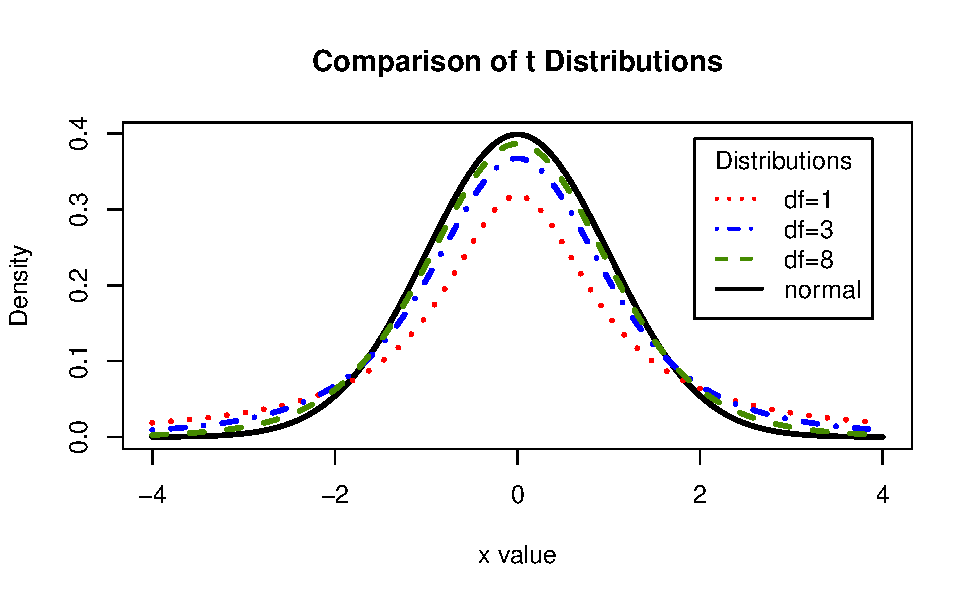
\includegraphics[width=0.7\linewidth]{11-A23-paired-theory_files/figure-latex/tdist-1} 

}

\caption{Comparison of the standard Normal vs t-distribution with various degrees of freedom}\label{fig:tdist}
\end{figure}

Like we saw in Chapter \textbf{5}, we will not know the values of the parameters and must use the sample data to estimate them. Unlike with proportions, in which we only needed to estimate the population proportion, \(\pi\), quantitative sample data must be used to estimate both a population mean \(\mu\) and a population standard deviation \(\sigma\). This additional uncertainty will require us to use a theoretical distribution that is just a bit wider than the Normal distribution. Enter the \textbf{\(t\)-distribution}!

As you can seen from Figure \ref{fig:tdist}, the \(t\)-distributions (dashed and dotted lines) are centered at 0 just like a standard Normal distribution (solid line), but are slightly wider. The variability of a \(t\)-distribution depends on its degrees of freedom, which is calculated from the sample size of a study. (For a single sample of \(n\) observations or paired differences, the degrees of freedom is equal to \(n-1\).) Recall from previous classes that larger sample sizes tend to result in narrower sampling distributions. We see that here as well. The larger the sample size, the larger the degrees of freedom, the narrower the \(t\)-distribution. (In fact, a \(t\)-distribution with infinite degrees of freedom actually IS the standard Normal distribution!)

\subsubsection*{Summarize and visualize the data}\label{summarize-and-visualize-the-data}
\addcontentsline{toc}{subsubsection}{Summarize and visualize the data}

Since the original data from the study are not available, we simulated data to match the means and standard deviations reported in the article. We will use these simulated data in the analysis below.

The following code plots each subject's time to read the colored words (above) and time to read the black words (below) connected by a grey line, a histogram of the differences in time to read words between the two conditions, and a boxplot displaying the pairwise differences in time (color \(-\) black).

\begin{itemize}
\item
  Download the R script file for this activity and upload to the R studio server.
\item
  Follow the instructions given in the R file.
\end{itemize}

\begin{Shaded}
\begin{Highlighting}[]
\NormalTok{color }\OtherTok{\textless{}{-}} \FunctionTok{read.csv}\NormalTok{(}\StringTok{"https://math.montana.edu/courses/s216/data/interference.csv"}\NormalTok{)}
\FunctionTok{paired\_observed\_plot}\NormalTok{(color)}

\NormalTok{color\_diff }\OtherTok{\textless{}{-}}\NormalTok{ color }\SpecialCharTok{\%\textgreater{}\%} 
  \FunctionTok{mutate}\NormalTok{(}\AttributeTok{differences =}\NormalTok{ DiffCol}\SpecialCharTok{{-}}\NormalTok{Black)}
\NormalTok{color\_diff }\SpecialCharTok{\%\textgreater{}\%}
  \FunctionTok{ggplot}\NormalTok{(}\FunctionTok{aes}\NormalTok{(}\AttributeTok{x =}\NormalTok{ differences))}\SpecialCharTok{+}
  \FunctionTok{geom\_boxplot}\NormalTok{()}\SpecialCharTok{+}
  \FunctionTok{labs}\NormalTok{(}\AttributeTok{title=}\StringTok{"Boxplot of the Difference in Time to Read Words }
\StringTok{       Between Color and Black for College Undergraduates"}\NormalTok{,}
       \AttributeTok{x =} \StringTok{"Differences in time to read words (Color {-} Black)"}\NormalTok{)}
\end{Highlighting}
\end{Shaded}

\begin{center}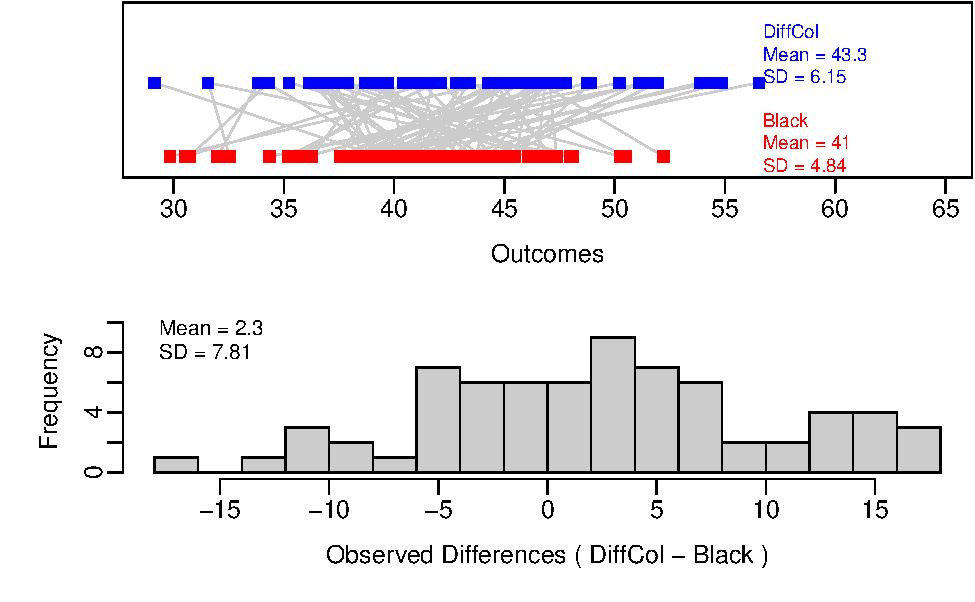
\includegraphics[width=0.7\linewidth]{11-A23-paired-theory_files/figure-latex/unnamed-chunk-1-1} 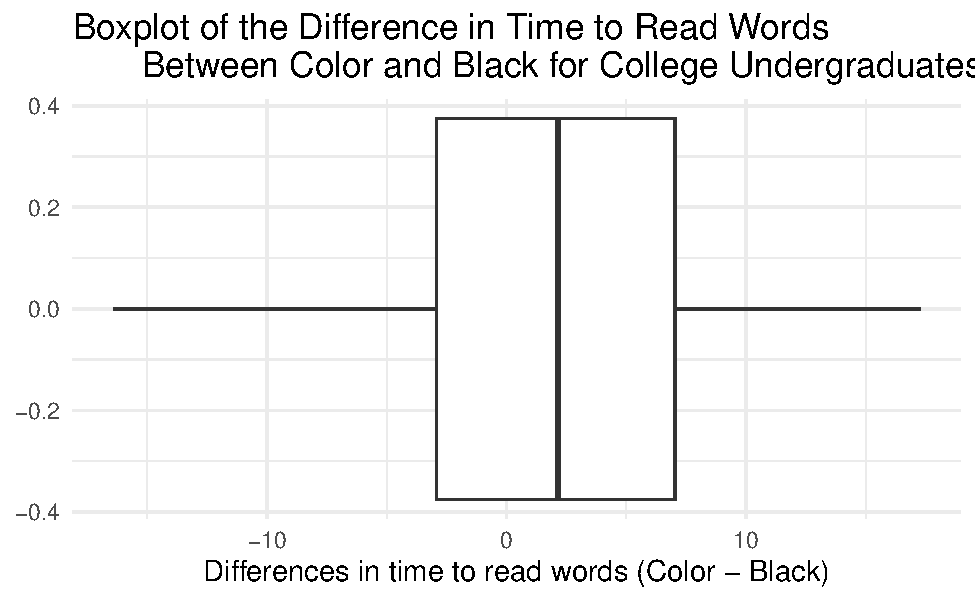
\includegraphics[width=0.7\linewidth]{11-A23-paired-theory_files/figure-latex/unnamed-chunk-1-2} \end{center}

The following code gives the summary statistics for the pairwise differences.

\begin{Shaded}
\begin{Highlighting}[]
\NormalTok{color\_diff }\SpecialCharTok{\%\textgreater{}\%} 
  \FunctionTok{summarise}\NormalTok{(}\FunctionTok{favstats}\NormalTok{(differences))}
\end{Highlighting}
\end{Shaded}

\begin{verbatim}
#>      min     Q1 median     Q3   max mean       sd  n missing
#> 1 -16.42 -2.925   2.15 7.0325 17.27  2.3 7.810196 70       0
\end{verbatim}

\subsubsection*{Check theoretical conditions}\label{check-theoretical-conditions}
\addcontentsline{toc}{subsubsection}{Check theoretical conditions}

\begin{enumerate}
\def\labelenumi{\arabic{enumi}.}
\setcounter{enumi}{4}
\item
  How do you know the independence condition is met for these data?
  \vspace{0.8in}
\item
  Is the normality condition met to use the theory-based methods for analysis? Explain your answer.
  \vspace{1in}
\end{enumerate}

\subsubsection*{Use statistical inferential methods to draw inferences from the data}\label{use-statistical-inferential-methods-to-draw-inferences-from-the-data-1}
\addcontentsline{toc}{subsubsection}{Use statistical inferential methods to draw inferences from the data}

To find the standardized statistic for the paired differences we will use the following formula:

\[T = \frac{\bar{x}_d - \mu_0}{SE(\bar{x}_d)},\]
where the standard error of the sample mean difference is:

\[SE(\bar{x}_d)=\frac{s_d}{\sqrt{n}}.\]

\begin{enumerate}
\def\labelenumi{\arabic{enumi}.}
\setcounter{enumi}{6}
\tightlist
\item
  Calculate the standard error of the sample mean difference.
\end{enumerate}

\vspace{0.5in}

\begin{enumerate}
\def\labelenumi{\arabic{enumi}.}
\setcounter{enumi}{7}
\tightlist
\item
  How many standard errors is the observed mean difference from the null mean difference?
\end{enumerate}

\vspace{0.5in}

To find the p-value

\begin{itemize}
\item
  Enter the value for the standardized statistic for xx in the pt function.
\item
  For a single sample or paired data, degrees of freedom are found by subtracting 1 from the sample size. You should therefore use \texttt{df} = \(n-1 = 70 - 1 = 69\) and \texttt{lower.tail\ =\ FALSE} to find the p-value.
\item
  Enter the df for yy in the pt function.
\item
  Highlight and run line 27
\end{itemize}

\begin{Shaded}
\begin{Highlighting}[]
\FunctionTok{pt}\NormalTok{(xx, }\AttributeTok{df=}\NormalTok{yy, }\AttributeTok{lower.tail=}\ConstantTok{FALSE}\NormalTok{)}
\end{Highlighting}
\end{Shaded}

\begin{enumerate}
\def\labelenumi{\arabic{enumi}.}
\setcounter{enumi}{8}
\tightlist
\item
  What does this p-value mean, in the context of the study? Hint: it is the probability of what\ldots assuming what?
  \vspace{1in}
\end{enumerate}

Next we will calculate a theory-based confidence interval. To calculate a theory-based confidence interval for the paired mean difference, use the following formula:

\[\bar{x}_d\pm t^* \times SE(\bar{x}_d).\]

We will need to find the \(t^*\) multiplier using the function \texttt{qt()}.

\begin{itemize}
\item
  Enter the appropriate percentile in the R code to find the multiplier for a 90\% confidence interval.
\item
  Enter the df for yy.
\end{itemize}

\begin{Shaded}
\begin{Highlighting}[]
\FunctionTok{qt}\NormalTok{(percentile, }\AttributeTok{df =}\NormalTok{ yy, }\AttributeTok{lower.tail=}\ConstantTok{TRUE}\NormalTok{)}
\end{Highlighting}
\end{Shaded}

\begin{enumerate}
\def\labelenumi{\arabic{enumi}.}
\setcounter{enumi}{10}
\tightlist
\item
  Mark on the t-distribution found below the values of \(\pm t^*\). Draw a line at each multiplier and write the percentiles used to find each.
  \vspace{1mm}
\end{enumerate}

\begin{figure}

{\centering 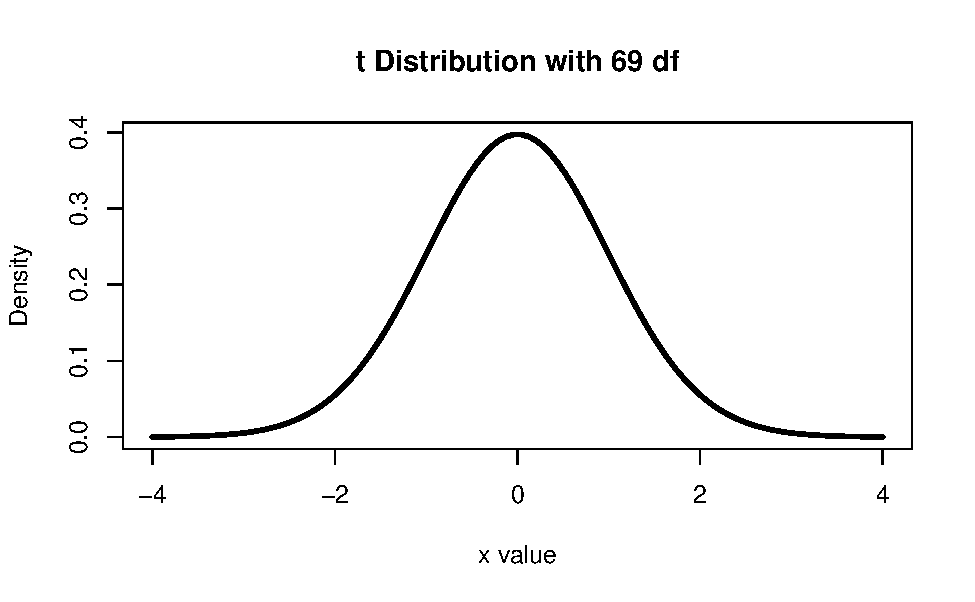
\includegraphics[width=0.7\linewidth]{11-A23-paired-theory_files/figure-latex/tstar-1} 

}

\caption{t-distribution with 69 degrees of freedom}\label{fig:tstar}
\end{figure}

\begin{enumerate}
\def\labelenumi{\arabic{enumi}.}
\setcounter{enumi}{11}
\tightlist
\item
  Calculate the margin of error for the true paired mean difference using theory-based methods.
\end{enumerate}

\vspace{0.6in}

\begin{enumerate}
\def\labelenumi{\arabic{enumi}.}
\setcounter{enumi}{12}
\tightlist
\item
  Calculate the confidence interval for the true paired mean difference using theory-based methods.
\end{enumerate}

\vspace{0.6in}

\begin{enumerate}
\def\labelenumi{\arabic{enumi}.}
\setcounter{enumi}{13}
\tightlist
\item
  Interpret the confidence interval in context of the study.
\end{enumerate}

\vspace{1in}

\begin{enumerate}
\def\labelenumi{\arabic{enumi}.}
\setcounter{enumi}{14}
\item
  Write a conclusion to the test in context of the study.
  \vspace{0.6in}
\item
  The abstract states, that the conflicting color stimuli ``caused an increase of 2.3 seconds or 5.6\% over the normal time for reading the same words printed in black.'' Is this statement valid? Explain.
  \vspace{0.6in}
\end{enumerate}

\subsection{Take-home messages}\label{take-home-messages-2}

\begin{enumerate}
\def\labelenumi{\arabic{enumi}.}
\item
  In order to use theory-based methods for dependent groups (paired data), the independent observational units and normality conditions must be met.
\item
  A T-score is compared to a \(t\)-distribution with \(n - 1\) df in order to calculate a one-sided p-value. To find a two-sided p-value using theory-based methods we need to multiply the one-sided p-value by 2.
\item
  A \(t^*\) multiplier is found by obtaining the bounds of the middle X\% (X being the desired confidence level) of a \(t\)-distribution with \(n - 1\) df.
\end{enumerate}

\subsection{Additional notes}\label{additional-notes-2}

Use this space to summarize your thoughts and take additional notes on today's activity and material covered

\newpage

\section{Module 11 Lab: Swearing}\label{module-11-lab-swearing}

\setstretch{1}

\subsection{Learning outcomes}\label{learning-outcomes-3}

\begin{itemize}
\item
  Identify whether a study is a paired design or independent groups
\item
  Given a research question involving paired data, construct the null and alternative hypotheses
  in words and using appropriate statistical symbols.
\item
  Describe and perform a simulation-based hypothesis test for a mean difference.
\item
  Interpret and evaluate a p-value for a hypothesis test for a mean difference.
\item
  Use bootstrapping methods to find a confidence interval for a mean difference.
\item
  Interpret a confidence interval for a mean difference.
\end{itemize}

\subsection{Swearing}\label{swearing}

Profanity (language considered obscene or taboo) and society's attitude about its acceptableness is a highly debated topic, but does swearing serve a physiological purpose or function? Previous research has shown that swearing produces increased heart rates and higher levels of skin conductivity. It is theorized that since swearing provokes intense emotional responses, it acts as a distracter, allowing a person to withstand higher levels of pain. To explore the relationship between swearing and increased pain tolerance, researchers from Keele University (Staffordshire, UK) recruited 83 native English-speaking participants (Stephens and Robertson 2020). Each volunteer performed two trials holding a hand in an ice-water bath, once while repeating the ``f-word'' every three seconds, and once while repeating a neutral word (``table''). The order of the word to repeat was randomly assigned. Researchers recorded the length of time, in seconds, from the moment the participant indicated they were in pain until they removed their hand from the ice water for each trial. They hope to find evidence that pain tolerance is greater (longer times) when a person swears compared to when they say a neutral word, on average. Use Swear -- Neutral as the order of subtraction.

\begin{enumerate}
\def\labelenumi{\arabic{enumi}.}
\tightlist
\item
  What is the explanatory variable for this study? What is the response?
\end{enumerate}

\vspace{0.5in}

\begin{enumerate}
\def\labelenumi{\arabic{enumi}.}
\setcounter{enumi}{1}
\tightlist
\item
  What does \(\mu_d\) represent in the context of this study?
\end{enumerate}

\vspace{0.8in}

\begin{enumerate}
\def\labelenumi{\arabic{enumi}.}
\setcounter{enumi}{2}
\tightlist
\item
  Write out the null hypothesis in proper notation for this study.
\end{enumerate}

\vspace{0.4in}

\begin{enumerate}
\def\labelenumi{\arabic{enumi}.}
\setcounter{enumi}{3}
\tightlist
\item
  What sign (\(<\), \(>\), or \(\neq\)) would you use in the alternative hypothesis for this study? Explain your choice.
\end{enumerate}

\vspace{0.5in}

\begin{itemize}
\item
  Upload and open the R script file for Week 12 lab.
\item
  Upload and import the csv file, \texttt{pain\_tolerance}.
\item
  Enter the name of the data set (see the environment tab) for datasetname in the R script file in line 8.
\item
  Highlight and run lines 1--9 to load the data and create a paired plot of the data.
\end{itemize}

\begin{Shaded}
\begin{Highlighting}[]
\NormalTok{swearing }\OtherTok{\textless{}{-}}\NormalTok{ datasetname}
\FunctionTok{paired\_observed\_plot}\NormalTok{(swearing)}
\end{Highlighting}
\end{Shaded}

\begin{enumerate}
\def\labelenumi{\arabic{enumi}.}
\setcounter{enumi}{4}
\tightlist
\item
  Based on the plots, does there appear to be some evidence in favor of the alternative hypothesis? How do you know?
  \vspace{0.4in}
\end{enumerate}

\begin{itemize}
\item
  Enter the outcome for group 1 (\texttt{Swear}) for \texttt{group\_1} and the outcome for group 2 (\texttt{Neutral}) for \texttt{group\_2} in line 16.
\item
  Highlight and run lines 14--25 to get the summary statistics and boxplot of the differences.
\end{itemize}

\begin{Shaded}
\begin{Highlighting}[]
\NormalTok{swearing\_diff }\OtherTok{\textless{}{-}}\NormalTok{ swearing }\SpecialCharTok{\%\textgreater{}\%} 
  \FunctionTok{mutate}\NormalTok{(}\AttributeTok{differences =}\NormalTok{ group\_1 }\SpecialCharTok{{-}}\NormalTok{ group\_2)}
\NormalTok{swearing\_diff }\SpecialCharTok{\%\textgreater{}\%} 
    \FunctionTok{summarise}\NormalTok{(}\FunctionTok{favstats}\NormalTok{(differences))}

\NormalTok{swearing\_diff }\SpecialCharTok{\%\textgreater{}\%} 
    \FunctionTok{ggplot}\NormalTok{(}\FunctionTok{aes}\NormalTok{(}\AttributeTok{x =}\NormalTok{ differences)) }\SpecialCharTok{+}
    \FunctionTok{geom\_boxplot}\NormalTok{()}\SpecialCharTok{+}
    \FunctionTok{labs}\NormalTok{(}\AttributeTok{title=}\StringTok{"Boxplot of the Difference in Time Participants Held Their Hand }
\StringTok{         in Ice Water while Swearing or while Saying a Neutral Word (Swearing {-} Neutral)"}\NormalTok{)}
\end{Highlighting}
\end{Shaded}

\begin{enumerate}
\def\labelenumi{\arabic{enumi}.}
\setcounter{enumi}{5}
\item
  What is the value of \(\bar{x}_d\)? What is the sample size?
  \vspace{0.25in}
\item
  \textbf{How far, on average, is each difference in time the participant holds their hand in ice water from the mean of the differences in time? What is the appropriate notation for this value?}
\end{enumerate}

\vspace{0.4in}

\subsection*{Use statistical inferential methods to draw inferences from the data}\label{use-statistical-inferential-methods-to-draw-inferences-from-the-data-2}
\addcontentsline{toc}{subsection}{Use statistical inferential methods to draw inferences from the data}

\begin{enumerate}
\def\labelenumi{\arabic{enumi}.}
\setcounter{enumi}{7}
\tightlist
\item
  Using the provided graphs and summary statistics, determine if both theory-based methods and simulation methods could be used to analyze the data. Explain your reasoning.
\end{enumerate}

\vspace{1in}

\subsection*{Hypothesis test}\label{hypothesis-test-1}
\addcontentsline{toc}{subsection}{Hypothesis test}

Remember that the null distribution is created based on the assumption the null hypothesis is true. In this study, the null hypothesis states that swearing does not affect pain tolerance, or that the length of time a subject kept their hand in the water would be the same whether the patient was swearing or not.

We will use the \texttt{paired\_test()} function in R (in the \texttt{catstats} package) to simulate the null distribution of sample mean differences and compute a p-value.

\newpage

\begin{enumerate}
\def\labelenumi{\arabic{enumi}.}
\setcounter{enumi}{8}
\tightlist
\item
  When using the \texttt{paired\_test()} function, we need to enter the name of the data set, either the order of subtraction (if the data set has both measurements) or the name of the differences (if the data set contains them). We will also need to provide R with the observed mean difference, the direction of the alternative hypothesis, and the shift required in order to force the null hypothesis to be true. The name of the data set as shown above is \texttt{swearing\_diff} and the column of differences is called \texttt{differences}. What values should be entered for each of the following to create 1000 simulated samples?
\end{enumerate}

\vspace{1mm}

\begin{itemize}
\tightlist
\item
  shift:
\end{itemize}

\vspace{.1in}

\begin{itemize}
\tightlist
\item
  As extreme as:
\end{itemize}

\vspace{.1in}

\begin{itemize}
\tightlist
\item
  Direction (\texttt{"greater"}, \texttt{"less"}, or \texttt{"two-sided"}):
\end{itemize}

\vspace{.1in}

\begin{itemize}
\tightlist
\item
  Number of repetitions:
\end{itemize}

\vspace{.1in}

\begin{enumerate}
\def\labelenumi{\arabic{enumi}.}
\setcounter{enumi}{9}
\tightlist
\item
  Simulate a null distribution and compute the p-value. Using the R script file for this lab, enter your answers for question 9 in place of the \texttt{xx}'s to produce the null distribution with 1000 simulations. Highlight and run lines 23--29.
\end{enumerate}

\begin{Shaded}
\begin{Highlighting}[]
\FunctionTok{paired\_test}\NormalTok{(}\AttributeTok{data =}\NormalTok{ swearing}\SpecialCharTok{$}\NormalTok{differences,   }\CommentTok{\# Vector of differences }
                                 \CommentTok{\# or data set with column for each group}
        \AttributeTok{shift =}\NormalTok{ xx,   }\CommentTok{\# Shift needed for bootstrap hypothesis test}
        \AttributeTok{as\_extreme\_as =}\NormalTok{ xx,  }\CommentTok{\# Observed statistic}
        \AttributeTok{direction =} \StringTok{"xx"}\NormalTok{,  }\CommentTok{\# Direction of alternative}
        \AttributeTok{number\_repetitions =}\NormalTok{ xx,  }\CommentTok{\# Number of simulated samples for null distribution}
        \AttributeTok{which\_first =} \DecValTok{1}\NormalTok{)  }\CommentTok{\# Not needed when using calculated differences}
\end{Highlighting}
\end{Shaded}

~~~~~~~Sketch the null distribution created using the \texttt{paired\_test} code.

\vspace{1.5in}

\subsection*{Communicate the results and answer the research question}\label{communicate-the-results-and-answer-the-research-question}
\addcontentsline{toc}{subsection}{Communicate the results and answer the research question}

\begin{enumerate}
\def\labelenumi{\arabic{enumi}.}
\setcounter{enumi}{10}
\tightlist
\item
  \textbf{Report the p-value. Based off of this p-value and a 1\% significance level, what decision would you make about the null hypothesis? What potential error might you be making based on that decision?}
\end{enumerate}

\vspace{0.5in}

\begin{enumerate}
\def\labelenumi{\arabic{enumi}.}
\setcounter{enumi}{11}
\tightlist
\item
  Do you expect the 98\% confidence interval to contain the null value of zero? Explain.
\end{enumerate}

\vspace{0.8in}

\subsection*{Confidence interval}\label{confidence-interval-2}
\addcontentsline{toc}{subsection}{Confidence interval}

We will use the \texttt{paired\_bootstrap\_CI()} function in R (in the \texttt{catstats} package) to simulate the bootstrap distribution of sample mean differences and calculate a confidence interval.

\begin{enumerate}
\def\labelenumi{\arabic{enumi}.}
\setcounter{enumi}{12}
\tightlist
\item
  Using bootstrapping and the provided R script file, find a 98\% confidence interval. Fill in the missing values/numbers in the \texttt{paired\_bootstrap\_CI()} function to create the 98\% confidence interval. Highlight and run lines 34--37. \textbf{Upload a copy of the bootstrap distribution created to Gradescope for your group.}
\end{enumerate}

\begin{Shaded}
\begin{Highlighting}[]
\FunctionTok{paired\_bootstrap\_CI}\NormalTok{(}\AttributeTok{data =}\NormalTok{ swearing\_diff}\SpecialCharTok{$}\NormalTok{differences, }\CommentTok{\# Enter vector of differences}
                    \AttributeTok{number\_repetitions =} \DecValTok{1000}\NormalTok{, }\CommentTok{\# Number of bootstrap samples for CI}
                    \AttributeTok{confidence\_level =}\NormalTok{ xx,  }\CommentTok{\# Confidence level in decimal form}
                    \AttributeTok{which\_first =} \DecValTok{1}\NormalTok{)  }\CommentTok{\# Not needed when entering vector of differences}
\end{Highlighting}
\end{Shaded}

Report the 98\% confidence interval in interval notation.

\vspace{0.3in}

\begin{enumerate}
\def\labelenumi{\arabic{enumi}.}
\setcounter{enumi}{13}
\tightlist
\item
  Interpret the \emph{confidence level} of the interval found in question 12.
\end{enumerate}

\vspace{0.8in}

\begin{enumerate}
\def\labelenumi{\arabic{enumi}.}
\setcounter{enumi}{14}
\tightlist
\item
  Write a paragraph summarizing the results of the study. \textbf{Upload a copy of your group's paragraph to Gradescope.} Be sure to describe:
\end{enumerate}

\begin{itemize}
\item
  Summary statistic and interpretation

  \begin{itemize}
  \item
    Summary measure (in context)
  \item
    Value of the statistic
  \item
    Order of subtraction when comparing two groups
  \end{itemize}
\item
  P-value and interpretation

  \begin{itemize}
  \item
    Statement about probability or proportion of samples
  \item
    Statistic (summary measure and value)
  \item
    Direction of the alternative
  \item
    Null hypothesis (in context)
  \end{itemize}
\item
  Confidence interval and interpretation

  \begin{itemize}
  \item
    How confident you are (e.g., 90\%, 95\%, 98\%, 99\%)
  \item
    Parameter of interest
  \item
    Calculated interval
  \item
    Order of subtraction when comparing two groups
  \end{itemize}
\item
  Conclusion (written to answer the research question)

  \begin{itemize}
  \item
    Amount of evidence
  \item
    Parameter of interest
  \item
    Direction of the alternative hypothesis
  \end{itemize}
\end{itemize}

\newpage

\begin{itemize}
\item
  Scope of inference

  \begin{itemize}
  \item
    To what group of observational units do the results apply (target population or observational units similar to the sample)?
  \item
    What type of inference is appropriate (causal or non-causal)?
  \end{itemize}
\end{itemize}

\newpage

\chapter{Inference for a Quantitative Response with Independent Samples}\label{inference-for-a-quantitative-response-with-independent-samples}

\section{Vocabulary Review and Key Topics}\label{vocabulary-review-and-key-topics-1}

Review the Golden Ticket posted in the resources at the end of the coursepack for a summary of a categorical explanatory variable and a quantitative response variable for independent samples. Module 12 will cover both simulation and theory-based methods of inference.

Types of plot for independent variables

\begin{itemize}
\item
  \textbf{Side-by-side boxplots}: plots a boxplot of the five number summary for each categorical level
\item
  R code to create side-by-side boxplots:
\end{itemize}

\begin{Shaded}
\begin{Highlighting}[]
\NormalTok{object }\SpecialCharTok{\%\textgreater{}\%}  \CommentTok{\# Data set piped into...}
  \FunctionTok{ggplot}\NormalTok{(}\FunctionTok{aes}\NormalTok{(}\AttributeTok{y =}\NormalTok{ response, }\AttributeTok{x =}\NormalTok{ explanatory))}\SpecialCharTok{+}  \CommentTok{\# Identify variables}
  \FunctionTok{geom\_boxplot}\NormalTok{()}\SpecialCharTok{+}  \CommentTok{\# Tell it to make a box plot}
  \FunctionTok{labs}\NormalTok{(}\AttributeTok{title =} \StringTok{"Don\textquotesingle{}t forget to include a title"}\NormalTok{,  }\CommentTok{\# Title: should include the type of plot,}
       \CommentTok{\# observational units, variables}
       \AttributeTok{x =} \StringTok{"x{-}axis label"}\NormalTok{,    }\CommentTok{\# x{-}axis label}
       \AttributeTok{y =} \StringTok{"y{-}axis label"}\NormalTok{)  }\CommentTok{\# y{-}axis label}
\end{Highlighting}
\end{Shaded}

\begin{itemize}
\item
  \textbf{Stacked histogram}: plots one histogram for each level of the categorical variable
\item
  \textbf{Stacked dotplots}: plots one dotplot for each level of the categorical variable
\item
  Four characteristics to compare boxplots

  \begin{itemize}
  \item
    Shape (symmetric or skewed)
  \item
    Center
  \item
    Spread
  \item
    Outliers?
  \end{itemize}
\end{itemize}

Summary measure

\begin{itemize}
\item
  \textbf{Difference in mean}: measures the difference in mean values between the two categorical groups
\item
  Parameter notation for difference in means: \(\mu_1 - \mu_2\), where 1 represents the 1st group of the explanatory variable and 2 represents the 2nd group
\item
  Sample notation for difference in means: \(\bar{x}_1 - \bar{x}_2\)
\end{itemize}

\vspace{1mm}

\begin{itemize}
\item
  R code to find the summary statistics

  \begin{itemize}
  \tightlist
  \item
    Note: review the interpretations of the other summary measures from Module 6
  \end{itemize}
\end{itemize}

\begin{Shaded}
\begin{Highlighting}[]
\NormalTok{object }\SpecialCharTok{\%\textgreater{}\%}
  \FunctionTok{reframe}\NormalTok{(}\FunctionTok{favstats}\NormalTok{(response}\SpecialCharTok{\textasciitilde{}}\NormalTok{explantory))}
\end{Highlighting}
\end{Shaded}

\subsection*{Simulation Hypothesis Testing}\label{simulation-hypothesis-testing-1}
\addcontentsline{toc}{subsection}{Simulation Hypothesis Testing}

Hypotheses:

\[H_0: \mu_1 - \mu_2 = 0 ~ \text{or}~ H_0: \mu_1 = \mu_2 \]
\[H_A: \mu_1 - \mu_2 \left\{
\begin{array}{ll}
< \\
\ne \\
< \\
\end{array}
\right\}
0 
~ \text{or} ~ H_A:
\mu_1 \left\{
\begin{array}{ll}
< \\
\ne \\
< \\
\end{array}
\right\}
\mu_2 \]

\begin{itemize}
\tightlist
\item
  R code for simulation methods to find the p-value using the \texttt{two\_mean\_test} function in the \texttt{catstats} package.
\end{itemize}

\begin{Shaded}
\begin{Highlighting}[]
\FunctionTok{two\_mean\_test}\NormalTok{(response}\SpecialCharTok{\textasciitilde{}}\NormalTok{explanatory, }\CommentTok{\#Enter the names of the variables }
               \AttributeTok{data =}\NormalTok{ object,  }\CommentTok{\# Enter the name of the dataset}
              \AttributeTok{first\_in\_subtraction =} \StringTok{"xx"}\NormalTok{, }\CommentTok{\# First outcome in order of subtraction }
               \AttributeTok{number\_repetitions =} \DecValTok{10000}\NormalTok{,  }\CommentTok{\# Number of simulations }
               \AttributeTok{as\_extreme\_as =} \SpecialCharTok{{-}}\NormalTok{xx,  }\CommentTok{\# Observed statistic }
               \AttributeTok{direction =} \StringTok{"xx"}\NormalTok{)  }\CommentTok{\# Direction of alternative: "greater", "less", or "two{-}sided"}
\end{Highlighting}
\end{Shaded}

\subsection*{Simulation Confidence Interval}\label{simulation-confidence-interval-1}
\addcontentsline{toc}{subsection}{Simulation Confidence Interval}

\begin{itemize}
\tightlist
\item
  R code to find the simulation confidence interval using the \texttt{twomean\_bootstrap\_CI} function from the \texttt{catstats} package.
\end{itemize}

\begin{Shaded}
\begin{Highlighting}[]
\FunctionTok{two\_mean\_bootstrap\_CI}\NormalTok{(response }\SpecialCharTok{\textasciitilde{}}\NormalTok{ explanatory, }\CommentTok{\#Enter the name of the variables}
                      \AttributeTok{data =}\NormalTok{ object,  }\CommentTok{\# Enter the name of the data set}
                      \AttributeTok{first\_in\_subtraction =} \StringTok{"xx"}\NormalTok{, }\CommentTok{\# First value in order of subtraction}
                      \AttributeTok{number\_repetitions =} \DecValTok{10000}\NormalTok{,  }\CommentTok{\# Number of simulations}
                      \AttributeTok{confidence\_level =}\NormalTok{ xx)}
\end{Highlighting}
\end{Shaded}

\begin{itemize}
\item
  Review how to interpret the confidence interval for two groups from Module 8
\item
  \textbf{Conditions for the sampling distribution of \(\bar{x}_1 - \bar{x}_2\) to follow an approximate normal distribution}:

  \begin{itemize}
  \item
    \textbf{Independence}: The sample's observations are independent, e.g., are from a simple random sample and there is independence between groups. (\emph{Remember}: This also must be true to use simulation methods!)
  \item
    \textbf{Large enough sample size: Normality Condition}: The sample observations come from a normally distributed population. Need to check for each group by using the following rules of thumb:

    \begin{itemize}
    \item
      \(n < 30\): Each distribution of the sample must be approximately normal with no outliers
    \item
      \(30 \ge n < 100\): We can relax the condition a little; the distribution of each sample must have no extreme outliers or skewness
    \item
      \(n > 100\): Can assume the sampling distribution of \(\bar{x}_1 - \bar{x}_2\) is nearly normal, even if the underlying distribuion of individual observations is not
    \end{itemize}
  \end{itemize}
\item
  \textbf{t-distribution}: a theoretical distribution that is symmetric with a given degrees of freedom smallest sample size minus 1 (\(n-1\))

  \begin{itemize}
  \tightlist
  \item
    \(t_{n-1}\)
  \end{itemize}
\end{itemize}

\newpage

\section{Video Notes: Inference for Independent Samples}\label{video-notes-inference-for-independent-samples}

Read Chapters 19 and 20 in the course textbook. Use the following videos to complete the video notes for Module 10.

\subsection{Course Videos}\label{course-videos-1}

\begin{itemize}
\item
  19.1
\item
  19.2
\item
  19.3TheoryTests
\item
  19.4TheoryInterval
\end{itemize}

\setstretch{1}

\subsection*{Single categorical, single quantitative variable with independent samples}\label{single-categorical-single-quantitative-variable-with-independent-samples}
\addcontentsline{toc}{subsection}{Single categorical, single quantitative variable with independent samples}

\setstretch{1.5}

\begin{itemize}
\item
  In this module, we will study inference for a \_\_\_\_\_\_\_\_\_\_\_\_\_\_\_\_\_\_\_\_\_\_ explanatory variable and a \_\_\_\_\_\_\_\_\_\_\_\_\_\_\_\_\_\_\_\_\_\_\_\_\_ response variable where the two groups are \_\_\_\_\_\_\_\_\_\_\_\_\_\_\_\_\_\_\_\_\_\_\_\_\_\_\_\_.
\item
  Independent groups: When the measurements in one sample are not
  related to the measurements in the other sample.
\end{itemize}

\setstretch{1}

\begin{itemize}
\item
  Two random samples taken separately from two populations and the same response variable is recorded. Compare the average number of sick days off from work for people who had a flu shot and people who didn't.
\item
  Participants are randomly assigned to one of two treatment conditions, and the same response variable is recorded.
\end{itemize}

Rather than analyzing the differences as a single mean we will calculate summary statistics on each sample.

Example: Fifty-one (51) college students volunteered to look at impacts on memorization, specifically if putting letters into recognizable patterns (like FBI, CIA, EDA, CDC, etc.) would increase the number letters memorized. (Miller 1956) The college students were randomly assigned to either a recognizable or non-recognizable letter group. After a period of study time, the number of letters memorized was collected on each study. Is there evidence that putting letters into recognizable letter groups improve memory?

\setstretch{1.5}

\begin{itemize}
\tightlist
\item
  The summary measure for two independent groups is the \_\_\_\_\_\_\_\_\_\_\_\_\_\_\_\_\_\_\_\_\_\_ in \_\_\_\_\_\_\_\_\_\_\_\_\_\_\_\_\_\_\_\_\_\_\_\_\_\_\_\_\_.
\end{itemize}

\setstretch{1}

\setstretch{1.5}

Notation for Independent Groups

\begin{itemize}
\item
  Population mean for group 1:
\item
  Population mean for group 2:
\item
  Sample mean for group 1:
\item
  Sample mean for group 2:
\item
  Sample difference in means:
\item
  Population standard deviation for group 1:
\item
  Population standard deviation for group 2:
\item
  Sample standard deviation for group 1:
\item
  Sample standard deviation for group 2:
\item
  Sample size for group 1:
\item
  Sample size for group 2:
\end{itemize}

\setstretch{1}

Why should we treat this as two independent groups rather than paired data?

\vspace{0.6in}

\subsection*{Hypothesis Testing}\label{hypothesis-testing-1}
\addcontentsline{toc}{subsection}{Hypothesis Testing}

Conditions:

\begin{itemize}
\tightlist
\item
  Independence: the response for one observational unit will not influence the outcome for another observational unit
\end{itemize}

Null hypothesis assumes ``no effect'', ``no difference'', ``nothing interesting happening'', etc.

\rgi Always of form: ``parameter'' = null value

\(H_0:\)

\vspace{0.5in}

\(H_A:\)

\vspace{0.5in}

\begin{itemize}
\tightlist
\item
  Research question determines the alternative hypothesis.
\end{itemize}

Write the null and alternative hypotheses for the letters study:

In notation:

\(H_0:\)

\vspace{0.2in}

\(H_A:\)

\vspace{0.2in}

\begin{Shaded}
\begin{Highlighting}[]
\NormalTok{letters}\OtherTok{\textless{}{-}}\FunctionTok{read.csv}\NormalTok{(}\StringTok{"data/letters.csv"}\NormalTok{)}
\NormalTok{letters }\SpecialCharTok{\%\textgreater{}\%}
    \FunctionTok{reframe}\NormalTok{(}\FunctionTok{favstats}\NormalTok{(Memorized}\SpecialCharTok{\textasciitilde{}}\NormalTok{Grouped))}
\end{Highlighting}
\end{Shaded}

\begin{verbatim}
#>           Grouped min Q1 median    Q3 max     mean       sd  n missing
#> 1 NotRecognizable   1  6     12 14.75  24 11.15385 6.576883 26       0
#> 2    Recognizable   1  6     15 21.00  30 14.32000 8.518216 25       0
\end{verbatim}

Summary statistic:

\vspace{0.4in}

Interpret the summary statistic in context of the problem:

\vspace{0.4in}

\begin{Shaded}
\begin{Highlighting}[]
\NormalTok{letters}\SpecialCharTok{\%\textgreater{}\%}
  \FunctionTok{ggplot}\NormalTok{(}\FunctionTok{aes}\NormalTok{(}\AttributeTok{y =}\NormalTok{ Memorized, }\AttributeTok{x =}\NormalTok{ Grouped))  }\SpecialCharTok{+} \CommentTok{\#Enter the name of the explanatory and response variable}
  \FunctionTok{geom\_boxplot}\NormalTok{()}\SpecialCharTok{+}
  \FunctionTok{labs}\NormalTok{(}\AttributeTok{title =} \StringTok{"Boxplot of Number of Letters memorized by Type }
\StringTok{       of Grouping for College Students"}\NormalTok{, }\CommentTok{\#Title your plot}
       \AttributeTok{y =} \StringTok{"Number of letters memorized"}\NormalTok{, }\CommentTok{\#y{-}axis label}
       \AttributeTok{x =} \StringTok{"Letter Grouping"}\NormalTok{) }\CommentTok{\#x{-}axis label}
\end{Highlighting}
\end{Shaded}

\begin{center}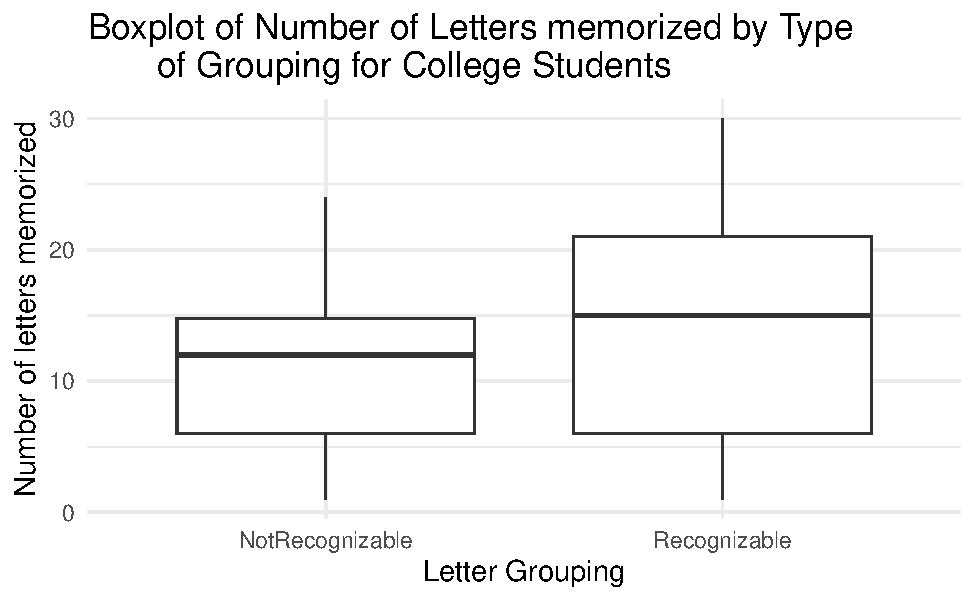
\includegraphics[width=0.6\linewidth]{12-VN12-1ofeach_files/figure-latex/unnamed-chunk-2-1} \end{center}

\subsubsection*{Simulation-based method}\label{simulation-based-method-2}
\addcontentsline{toc}{subsubsection}{Simulation-based method}

\begin{itemize}
\item
  Simulate many samples assuming \(H_0: \mu_1 = \mu_2\)

  \begin{itemize}
  \item
    Write the response variable values on cards
  \item
    Mix the explanatory variable groups together
  \item
    Shuffle cards into two explanatory variable groups to represent the sample size in each group (\(n_1\) and \(n_2\))
  \item
    Calculate and plot the simulated difference in sample means from each simulation
  \item
    Repeat 1000 times (simulations) to create the null distribution
  \item
    Find the proportion of simulations at least as extreme as \(\bar{x}_1 - \bar{x}_2\)
  \end{itemize}
\end{itemize}

\vspace{1mm}

\begin{Shaded}
\begin{Highlighting}[]
\FunctionTok{set.seed}\NormalTok{(}\DecValTok{216}\NormalTok{)}
\FunctionTok{two\_mean\_test}\NormalTok{(Memorized}\SpecialCharTok{\textasciitilde{}}\NormalTok{Grouped, }\CommentTok{\#Enter the names of the variables}
              \AttributeTok{data =}\NormalTok{ letters,  }\CommentTok{\# Enter the name of the dataset}
              \AttributeTok{first\_in\_subtraction =} \StringTok{"Recognizable"}\NormalTok{, }\CommentTok{\# First outcome in order of subtraction}
              \AttributeTok{number\_repetitions =} \DecValTok{10000}\NormalTok{,  }\CommentTok{\# Number of simulations}
              \AttributeTok{as\_extreme\_as =} \FloatTok{3.166}\NormalTok{,  }\CommentTok{\# Observed statistic}
              \AttributeTok{direction =} \StringTok{"greater"}\NormalTok{)  }\CommentTok{\# Direction of alternative: "greater", "less", or "two{-}sided"}
\end{Highlighting}
\end{Shaded}

\begin{center}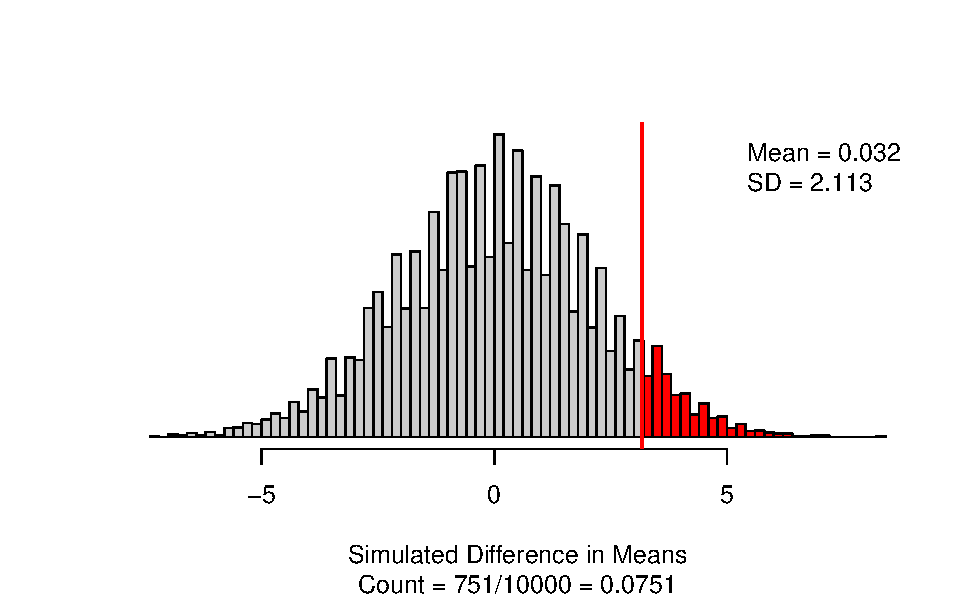
\includegraphics[width=0.7\linewidth]{12-VN12-1ofeach_files/figure-latex/unnamed-chunk-3-1} \end{center}

Explain why the null distribution is centered at the value of zero:

\vspace{0.8in}

Interpretation of the p-value:

\begin{itemize}
\item
  Statement about probability or proportion of samples
\item
  Statistic (summary measure and value)
\item
  Direction of the alternative
\item
  Null hypothesis (in context)
\end{itemize}

\vspace{0.8in}

Conclusion:

\begin{itemize}
\item
  Amount of evidence
\item
  Parameter of interest
\item
  Direction of the alternative hypothesis
\end{itemize}

\vspace{0.6in}

\newpage

\subsection*{Confidence interval}\label{confidence-interval-3}
\addcontentsline{toc}{subsection}{Confidence interval}

To estimate the difference in true mean we will create a confidence interval.

\subsubsection*{Simulation-based method - Video 19.2}\label{simulation-based-method---video-19.2}
\addcontentsline{toc}{subsubsection}{Simulation-based method - Video 19.2}

\begin{itemize}
\item
  Write the response variable values on cards
\item
  Keep explanatory variable groups separate
\item
  Sample with replacement \(n_1\) times in explanatory variable group 1 and \(n_2\) times in explanatory variable group 2
\item
  Calculate and plot the simulated difference in sample means from each simulation
\item
  Repeat 1000 times (simulations) to create the bootstrap distribution
\item
  Find the cut-offs for the middle X\% (confidence level) in a bootstrap distribution.
\end{itemize}

For the letters example, we will estimate the difference in true mean number of letters recognized for students given recognizable letter groupings and students given non-recognizable letter groupings.

\begin{Shaded}
\begin{Highlighting}[]
\FunctionTok{set.seed}\NormalTok{(}\DecValTok{216}\NormalTok{)}
\FunctionTok{two\_mean\_bootstrap\_CI}\NormalTok{(Memorized }\SpecialCharTok{\textasciitilde{}}\NormalTok{ Grouped, }\CommentTok{\#Enter the name of the variables}
                      \AttributeTok{data =}\NormalTok{ letters,  }\CommentTok{\# Enter the name of the data set}
                      \AttributeTok{first\_in\_subtraction =} \StringTok{"Recognizable"}\NormalTok{, }\CommentTok{\# First value in order of subtraction}
                      \AttributeTok{number\_repetitions =} \DecValTok{10000}\NormalTok{,  }\CommentTok{\# Number of simulations}
                      \AttributeTok{confidence\_level =} \FloatTok{0.95}\NormalTok{)}
\end{Highlighting}
\end{Shaded}

\begin{center}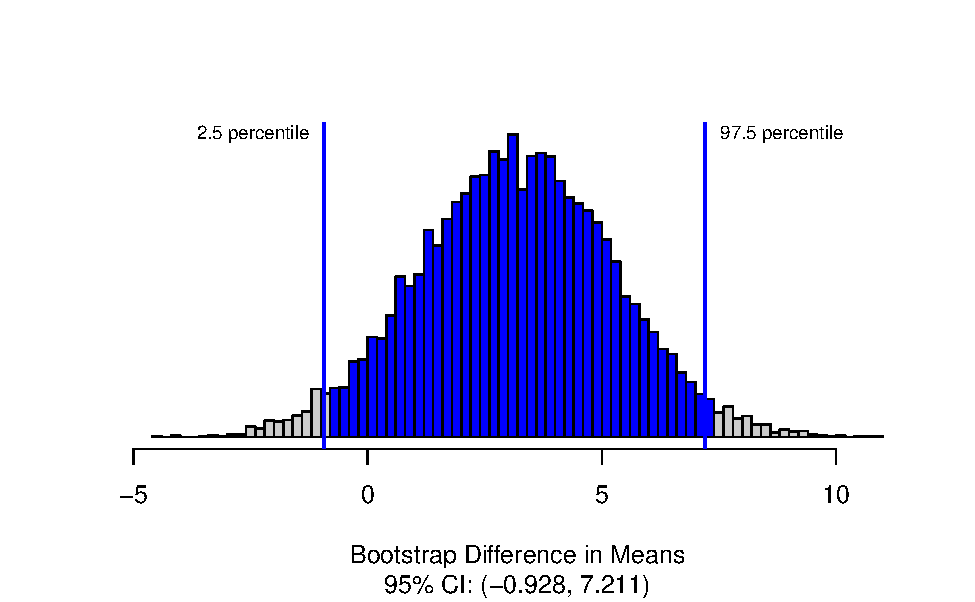
\includegraphics[width=0.7\linewidth]{12-VN12-1ofeach_files/figure-latex/unnamed-chunk-4-1} \end{center}

Confidence interval interpretation:

\begin{itemize}
\item
  How confident you are (e.g., 90\%, 95\%, 98\%, 99\%)
\item
  Parameter of interest
\item
  Calculated interval
\item
  Order of subtraction when comparing two groups
\end{itemize}

\vspace{0.8in}

\subsubsection*{Theory-based method - Video 19.3TheoryTests}\label{theory-based-method---video-19.3theorytests}
\addcontentsline{toc}{subsubsection}{Theory-based method - Video 19.3TheoryTests}

Example: Every year, orange and black monarch butterflies migrate from their summer breeding grounds in the US and Canada to mountain forests in central Mexico, where they hibernate for the winter. Due to abnormal weather patterns and drought affecting monarch habitats and feeding grounds, the population of monarch butterflies is estimated to have decreased by 53\% from the 2018-2019 wintering season to the 2019-2020 wintering season (WWF, 2020). While conservationists often resort to captive-rearing with the goal of raising biologically indistinct individuals for release into the wild, tagging studies have shown that captive-reared monarchs have lower migratory success compared to wild monarchs. For this study, the researchers raised 67 monarchs (descended from wild monarchs) from eggs to maturity and then compared them to a group of 40 wild-caught monarchs. The researchers want to explore whether the maximum grip strength (how many Newtons a butterfly exerts at the moment of release when gently tugged from a mesh-covered perch) differs between captive-reared and wild-caught monarchs. Use Captive -- Wild for order of subtraction.

Write the null and alternative hypotheses in notation.

\(H_0:\)

\vspace{0.2in}

\(H_A:\)

\vspace{0.2in}

\begin{Shaded}
\begin{Highlighting}[]
\NormalTok{butterfly }\OtherTok{\textless{}{-}}\FunctionTok{read.csv}\NormalTok{(}\StringTok{"data/butterfly1.csv"}\NormalTok{)}

\NormalTok{butterflies }\OtherTok{\textless{}{-}}\NormalTok{ butterfly }\SpecialCharTok{\%\textgreater{}\%} \FunctionTok{na.omit}\NormalTok{() }\SpecialCharTok{\%\textgreater{}\%}
    \FunctionTok{rename}\NormalTok{(}\AttributeTok{Monarch\_Group =} \StringTok{"Monarch.Group"}\NormalTok{,}
           \AttributeTok{MaxGrip =} \StringTok{"Max.Grip.Strength..N."}\NormalTok{) }\SpecialCharTok{\%\textgreater{}\%}
    \FunctionTok{mutate}\NormalTok{(}\AttributeTok{Monarch\_Group =} \FunctionTok{factor}\NormalTok{(Monarch\_Group),}
           \AttributeTok{Sex =} \FunctionTok{factor}\NormalTok{(Sex)) }\SpecialCharTok{\%\textgreater{}\%}
    \FunctionTok{mutate}\NormalTok{(}\AttributeTok{Monarch\_Group =} \FunctionTok{fct\_collapse}\NormalTok{(Monarch\_Group,}\StringTok{"Captive"} \OtherTok{=} \FunctionTok{c}\NormalTok{(}\StringTok{"Incubator {-} Fall conditions"}\NormalTok{, }\StringTok{"Rearing room {-} summer conditions"}\NormalTok{), }\StringTok{"Wild"} \OtherTok{=} \StringTok{"Wild migrants"}\NormalTok{))}

\NormalTok{butterflies }\SpecialCharTok{\%\textgreater{}\%}
    \FunctionTok{reframe}\NormalTok{(}\FunctionTok{favstats}\NormalTok{(MaxGrip}\SpecialCharTok{\textasciitilde{}}\NormalTok{Monarch\_Group))}
\end{Highlighting}
\end{Shaded}

\begin{verbatim}
#>   Monarch_Group   min    Q1 median     Q3   max      mean         sd  n missing
#> 1       Captive 0.081 0.162  0.217 0.2845 0.596 0.2363731 0.09412948 67       0
#> 2          Wild 0.108 0.271  0.352 0.4330 0.650 0.3607500 0.14066796 40       0
\end{verbatim}

\begin{center}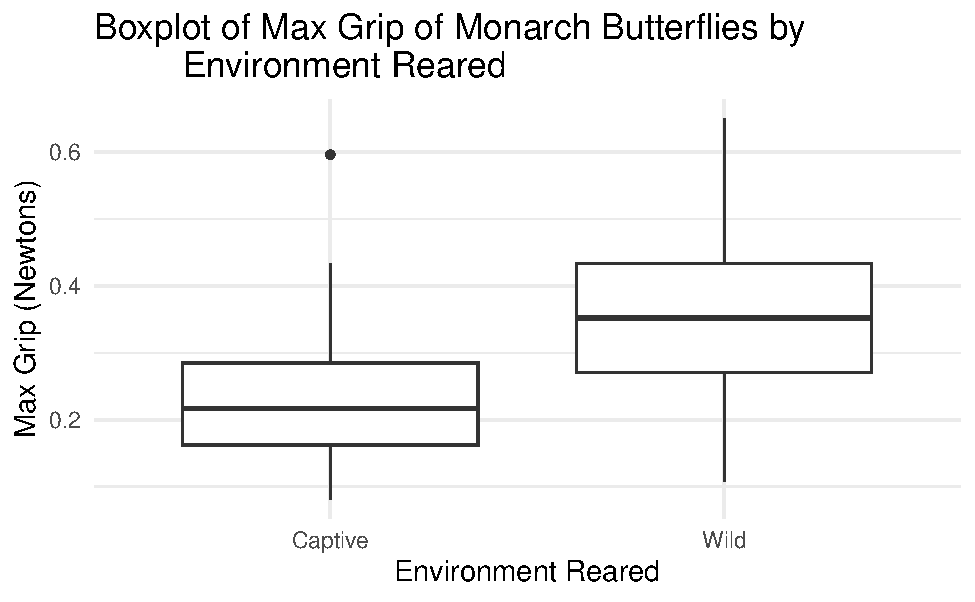
\includegraphics[width=0.7\linewidth]{12-VN12-1ofeach_files/figure-latex/unnamed-chunk-6-1} \end{center}

Conditions:

\begin{itemize}
\item
  Independence: the response for one observational unit will not influence the outcome for another observational unit
\item
  Large enough sample size
\end{itemize}

\vspace{1in}

Like with paired data the t-distribution can be used to model the difference in means.

\setstretch{1.5}

\begin{itemize}
\tightlist
\item
  For independent samples we use the \_\_\_\_\_\_- distribution
  with \_\_\_\_\_\_\_\_\_\_\_\_\_\_\_\_ degrees of freedom to approximate the sampling distribution.
\end{itemize}

\setstretch{1}

Theory-based test:

\begin{itemize}
\item
  Calculate the standardized statistic
\item
  Find the area under the t-distribution with the smallest \(n - 1\) df {[}min(\(n_1-1, n_2-1\)){]} at least as extreme as the standardized statistic
\end{itemize}

Equation for the standard error of the difference in sample mean:

\vspace{0.5in}

Equation for the standardized difference in sample mean:

\vspace{0.5in}

Are the conditions met to analyze the butterfly data using theory based-methods?

\vspace{0.8in}

Calculate the standardized difference in mean max grip strength.

\begin{itemize}
\tightlist
\item
  First calculate the \(SE(\bar{x}_1 - \bar{x}_2)\)
\end{itemize}

\vspace{0.6in}

\begin{itemize}
\tightlist
\item
  Then calculate the T-score
\end{itemize}

\vspace{1in}

What theoretical distribution should we use to find the p-value?

\vspace{0.3in}

To find the theory-based p-value:

\begin{Shaded}
\begin{Highlighting}[]
\FunctionTok{pt}\NormalTok{(}\SpecialCharTok{{-}}\DecValTok{5}\NormalTok{, }\AttributeTok{df=}\DecValTok{39}\NormalTok{, }\AttributeTok{lower.tail=}\ConstantTok{FALSE}\NormalTok{)}\SpecialCharTok{*}\DecValTok{2}
\end{Highlighting}
\end{Shaded}

\begin{verbatim}
#> [1] 1.999987
\end{verbatim}

Conclusion:

\begin{itemize}
\item
  Amount of evidence
\item
  Parameter of interest
\item
  Direction of the alternative hypothesis
\end{itemize}

\vspace{0.6in}

\subsubsection*{Confidence Interval - Video 19.3TheoryIntervals}\label{confidence-interval---video-19.3theoryintervals}
\addcontentsline{toc}{subsubsection}{Confidence Interval - Video 19.3TheoryIntervals}

\begin{itemize}
\tightlist
\item
  Calculate the interval centered at the sample statistic
\end{itemize}

\rgi \(\text{statistic} \pm \text{margin of error}\)

\vspace{0.8in}

Using the butterfly data, calculate the 99\% confidence interval.

\begin{Shaded}
\begin{Highlighting}[]
\NormalTok{butterflies }\SpecialCharTok{\%\textgreater{}\%}
    \FunctionTok{reframe}\NormalTok{(}\FunctionTok{favstats}\NormalTok{(MaxGrip}\SpecialCharTok{\textasciitilde{}}\NormalTok{Monarch\_Group))}
\end{Highlighting}
\end{Shaded}

\begin{verbatim}
#>   Monarch_Group   min    Q1 median     Q3   max      mean         sd  n missing
#> 1       Captive 0.081 0.162  0.217 0.2845 0.596 0.2363731 0.09412948 67       0
#> 2          Wild 0.108 0.271  0.352 0.4330 0.650 0.3607500 0.14066796 40       0
\end{verbatim}

\begin{itemize}
\tightlist
\item
  Need the \(t^*\) multiplier for a 99\% confidence interval from a t-distribution with \_\_\_\_\_\_\_\_\_ df.
\end{itemize}

\begin{Shaded}
\begin{Highlighting}[]
\FunctionTok{qt}\NormalTok{(}\FloatTok{0.995}\NormalTok{, }\AttributeTok{df=}\DecValTok{39}\NormalTok{, }\AttributeTok{lower.tail =} \ConstantTok{TRUE}\NormalTok{)}
\end{Highlighting}
\end{Shaded}

\begin{verbatim}
#> [1] 2.707913
\end{verbatim}

\begin{itemize}
\tightlist
\item
  We will use the same value for the \(SE(\bar{x}_1-\bar{x}_2)\) as calculated for the standardized statistic.
\end{itemize}

\vspace{1in}

Calculate the margin of error for a 99\% confidence interval for the parameter of interest.

\vspace{0.5in}

Calculate a 99\% confidence interval for the parameter of interest.

\vspace{0.6in}

\subsection{Concept Check}\label{concept-check-1}

Be prepared for group discussion in the next class. One member from the table should write the answers to the following on the whiteboard.

\begin{enumerate}
\def\labelenumi{\arabic{enumi}.}
\tightlist
\item
  Why is the recognizable letter study analyzed as two independent groups rather than paired data?
\end{enumerate}

\vspace{0.6in}

\begin{enumerate}
\def\labelenumi{\arabic{enumi}.}
\setcounter{enumi}{1}
\tightlist
\item
  Write out the equation for the standard error for a difference in sample means.
\end{enumerate}

\vspace{1in}

\newpage

\section{Activity 24: Does behavior impact performance?}\label{activity-24-does-behavior-impact-performance}

\setstretch{1}

\subsection{Learning outcomes}\label{learning-outcomes-4}

\begin{itemize}
\tightlist
\item
  Create a side-by-side boxplot of one categorical explanatory variable and one quantitative response variable
\end{itemize}

\begin{itemize}
\item
  Use bootstrapping to find a confidence interval for a difference in means.
\item
  Interpret a confidence interval for a difference in means.
\item
  Use a confidence interval to determine the conclusion of a hypothesis test.
\end{itemize}

\subsection{Terminology review}\label{terminology-review-3}

In today's activity, we will use simulation-based methods to analyze the association between one categorical explanatory variable and one quantitative response variable, where the groups formed by the categorical variable are independent. Some terms covered in this activity are:

\begin{itemize}
\item
  Independent groups
\item
  Difference in means
\end{itemize}

To review these concepts, see Chapter 19 in the textbook.

\subsection{Behavior and Performance}\label{behavior-and-performance}

A study in the Academy of Management Journal (Porath 2017) investigated how rude behaviors influence a victim's task performance. Randomly selected college students enrolled in a management course were randomly assigned to one of two experimental conditions: rudeness condition (45 students) and control group (53 students). Each student was asked to write down as many uses for a brick as possible in five minutes; this value (total number of uses) was used as a performance measure for each student, where higher values indicate better performance. During this time another individual showed up late for class. For those students in the rudeness condition, the facilitator displayed rudeness by berating the students in general for being irresponsible and unprofessional (due to the late-arriving person). No comments were made about the late-arriving person for students in the control group. Is there evidence that the average performance score for students in the rudeness condition is lower than for students in the control group? Use the order of subtraction of rudeness -- control.

\begin{Shaded}
\begin{Highlighting}[]
\CommentTok{\# Read in data set}
\NormalTok{rude }\OtherTok{\textless{}{-}} \FunctionTok{read.csv}\NormalTok{(}\StringTok{"https://math.montana.edu/courses/s216/data/rude.csv"}\NormalTok{)}
\end{Highlighting}
\end{Shaded}

\newpage

\begin{Shaded}
\begin{Highlighting}[]
\CommentTok{\# Side{-}by{-}side box plots}
\NormalTok{rude }\SpecialCharTok{\%\textgreater{}\%}
\FunctionTok{ggplot}\NormalTok{(}\FunctionTok{aes}\NormalTok{(}\AttributeTok{x =}\NormalTok{ condition, }\AttributeTok{y =}\NormalTok{ number\_of\_uses)) }\SpecialCharTok{+}
    \FunctionTok{geom\_boxplot}\NormalTok{() }\SpecialCharTok{+} 
    \FunctionTok{labs}\NormalTok{(}\AttributeTok{title =} \StringTok{"Number of Uses for a Brick based on Behavior Condition}
\StringTok{         for College Students in a Management Course"}\NormalTok{,}
         \AttributeTok{x =} \StringTok{"Behavior"}\NormalTok{) }
\end{Highlighting}
\end{Shaded}

\begin{center}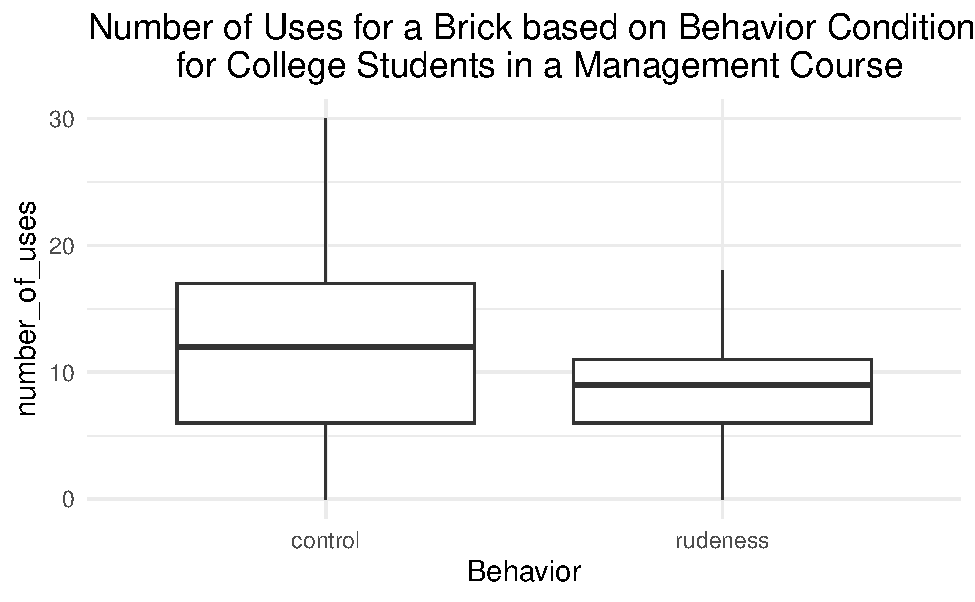
\includegraphics[width=0.6\linewidth]{12-A24-inference-1ofeach-simulation_files/figure-latex/unnamed-chunk-2-1} \end{center}

\begin{Shaded}
\begin{Highlighting}[]
\CommentTok{\# Summary statistics}
\NormalTok{rude }\SpecialCharTok{\%\textgreater{}\%} 
     \FunctionTok{reframe}\NormalTok{(}\FunctionTok{favstats}\NormalTok{(number\_of\_uses }\SpecialCharTok{\textasciitilde{}}\NormalTok{ condition))}
\end{Highlighting}
\end{Shaded}

\begin{verbatim}
#>   condition min Q1 median Q3 max      mean       sd  n missing
#> 1   control   0  6     12 17  30 11.811321 7.382559 53       0
#> 2  rudeness   0  6      9 11  18  8.511111 3.992164 45       0
\end{verbatim}

\subsubsection*{Quantitative variables review}\label{quantitative-variables-review}
\addcontentsline{toc}{subsubsection}{Quantitative variables review}

\begin{enumerate}
\def\labelenumi{\arabic{enumi}.}
\item
  Compare the distributions of the number of bricks between the two treatment conditions.

  \begin{itemize}
  \item
    What is the shape of each group?
    \vspace{0.3in}
  \item
    Which group has the higher center?
    \vspace{0.3in}
  \item
    What group has the larger spread?
    \vspace{0.3in}
  \item
    Does either distribution have outliers?
    \vspace{.3in}
  \end{itemize}
\item
  Is this an experiment or an observational study? Justify your answer.
\end{enumerate}

\vspace{1in}

\begin{enumerate}
\def\labelenumi{\arabic{enumi}.}
\setcounter{enumi}{2}
\tightlist
\item
  Explain why this is two independent samples and not paired data.
  \vspace{1in}
\end{enumerate}

\subsubsection*{Numerically Summarize the data}\label{numerically-summarize-the-data}
\addcontentsline{toc}{subsubsection}{Numerically Summarize the data}

\begin{enumerate}
\def\labelenumi{\arabic{enumi}.}
\setcounter{enumi}{3}
\tightlist
\item
  Calculate the summary statistic of interest (difference in means). What is the appropriate notation for this statistic?
\end{enumerate}

\vspace{0.5in}

Interpret this calculated value.

\vspace{0.6in}

\begin{enumerate}
\def\labelenumi{\arabic{enumi}.}
\setcounter{enumi}{4}
\item
  Write out the parameter of interest for this study in context of the study.

  \begin{itemize}
  \item
    To write in context:

    \begin{itemize}
    \item
      Population word (true, long-run, population)
    \item
      Summary measure (depends on the type of data)
    \item
      Context

      \begin{itemize}
      \item
        Observational units
      \item
        Variable(s)
        \vspace{1in}
      \end{itemize}
    \end{itemize}
  \end{itemize}
\end{enumerate}

\subsubsection*{Use statistical inferential methods to draw inferences from the data}\label{use-statistical-inferential-methods-to-draw-inferences-from-the-data-3}
\addcontentsline{toc}{subsubsection}{Use statistical inferential methods to draw inferences from the data}

\paragraph*{Confidence interval}\label{confidence-interval-4}
\addcontentsline{toc}{paragraph}{Confidence interval}

We will use the \texttt{two\_proportion\_bootstrap\_CI()} function in R (in the \texttt{catstats} package) to simulate the bootstrap distribution of differences in sample proportions and calculate a confidence interval. We will need to enter the response variable name and the explanatory variable name for the formula, the data set name (identified above as \texttt{rude}), the outcome for the explanatory variable that is first in subtraction, number of repetitions, the outcome for the response variable that is a success (the count for the numerator when calculating a sample proportion), and the confidence level as a decimal.

The response variable name is \texttt{number\_of\_uses} and the explanatory variable name is \texttt{condition}.

\begin{enumerate}
\def\labelenumi{\arabic{enumi}.}
\setcounter{enumi}{5}
\tightlist
\item
  What values should be entered for each of the following into the simulation to create a 99\% confidence interval?
  \vspace{.5mm}
\end{enumerate}

\begin{itemize}
\tightlist
\item
  First in subtraction (What is the outcome for the explanatory variable that is used as first in the order of subtraction? \texttt{"rudeness"} or \texttt{"control"}):
\end{itemize}

\vspace{.15in}

\begin{itemize}
\tightlist
\item
  Number of repetitions:
\end{itemize}

\vspace{.15in}

\begin{itemize}
\tightlist
\item
  Confidence level (entered as a decimal):
\end{itemize}

\vspace{.15in}

Using the R script file for this activity, enter your answers for question 6 in place of the \texttt{xx}'s to produce the bootstrap distribution with 1000 simulations; highlight and run lines 16--21.

\begin{Shaded}
\begin{Highlighting}[]
\FunctionTok{two\_mean\_bootstrap\_CI}\NormalTok{(response }\SpecialCharTok{\textasciitilde{}}\NormalTok{ explanatory, }\CommentTok{\#Enter the name of the variables}
                      \AttributeTok{data =}\NormalTok{ rude,  }\CommentTok{\# Enter the name of the data set}
                      \AttributeTok{first\_in\_subtraction =} \StringTok{"xx"}\NormalTok{, }\CommentTok{\# First value in order of subtraction}
                      \AttributeTok{number\_repetitions =} \DecValTok{1000}\NormalTok{,  }\CommentTok{\# Number of simulations}
                      \AttributeTok{confidence\_level =}\NormalTok{ xx)}
\end{Highlighting}
\end{Shaded}

\begin{enumerate}
\def\labelenumi{\arabic{enumi}.}
\setcounter{enumi}{6}
\tightlist
\item
  Where is the bootstrap distribution centered? Explain why.
\end{enumerate}

\vspace{0.8in}

\begin{enumerate}
\def\labelenumi{\arabic{enumi}.}
\setcounter{enumi}{7}
\tightlist
\item
  Report the bootstrap 99\% confidence interval.
\end{enumerate}

\vspace{0.4in}

\begin{enumerate}
\def\labelenumi{\arabic{enumi}.}
\setcounter{enumi}{8}
\tightlist
\item
  What percentile of the bootstrap distribution does the upper value of the confidence interval represent?
\end{enumerate}

\vspace{0.3in}

\begin{enumerate}
\def\labelenumi{\arabic{enumi}.}
\setcounter{enumi}{9}
\tightlist
\item
  Interpret the 99\% confidence interval.
\end{enumerate}

\vspace{1in}

\subsection{Take-home messages}\label{take-home-messages-3}

\begin{enumerate}
\def\labelenumi{\arabic{enumi}.}
\item
  This activity differs from the activities in Module 11 because the responses are independent, not paired. These data are analyzed as a difference in means, not a mean difference.
\item
  To create one simulated sample on the null distribution for a difference in sample means, label cards with the response variable values from the original data. Mix cards together and shuffle into two new groups of sizes \(n_1\) and \(n_2\). Calculate and plot the difference in means.
\item
  To create one simulated sample on the bootstrap distribution for a difference in sample means, label \(n_1 + n_2\) cards with the original response values. Keep groups separate and randomly draw with replacement \(n_1\) times from group 1 and \(n_2\) times from group 2. Calculate and plot the resampled difference in means.
\end{enumerate}

\subsection{Additional notes}\label{additional-notes-3}

Use this space to summarize your thoughts and take additional notes on today's activity and material covered

\newpage

\section{Activity 25: Moon Phases and Virtual Reality}\label{activity-25-moon-phases-and-virtual-reality}

\setstretch{1}

\subsection{Learning outcomes}\label{learning-outcomes-5}

\begin{itemize}
\item
  Given a research question involving one categorical explanatory variable and one quantitative response variable, construct the null and alternative hypotheses
  in words and using appropriate statistical symbols.
\item
  Describe and perform a theory-based hypothesis test for a difference in means.
\item
  Interpret and evaluate a p-value for a theory-based hypothesis test for a difference in means.
\item
  Use theory-based methods to find a confidence interval for a difference in means.
\item
  Interpret a confidence interval for a difference in means.
\item
  Use a confidence interval to determine the conclusion of a hypothesis test.
\end{itemize}

\subsection{Terminology review}\label{terminology-review-4}

In today's activity, we will use theory-based methods to analyze the association between one categorical explanatory variable and one quantitative response variable, where the groups formed by the categorical variable are independent. Some terms covered in this activity are:

\begin{itemize}
\item
  Difference in means
\item
  Independence within and between groups
\item
  Normality
\end{itemize}

To review these concepts, see Chapter 19 in the textbook.

\subsection{Moon Phases and Virtual Reality}\label{moon-phases-and-virtual-reality}

In a study comparing immersive virtual reality (VR) to traditional hands-on methods, researchers recruited 115 undergraduate students to assess the effectiveness of these approaches in teaching complex scientific concepts like Moon phases (Madden 2020). Participants were randomly assigned to experience either a VR simulation replicating the Sun-Earth-Moon system or a hands-on activity where they physically manipulated models to observe Moon phases. The students were given a 14 multiple choice question quiz about Moon phases and the Moon's motion relative to the Earth to evaluate their understanding of Moon phases and the Moon's motion. Each question had only one correct answer, and the participant's score was the sum of the number of correct answers, with all questions weighted equally (with a maximum score of 14). Is there evidence of a difference, on average, in student learning comparing those using VR methods to those using the traditional method? Use order of subtraction VR -- Hands-on.

\begin{enumerate}
\def\labelenumi{\arabic{enumi}.}
\item
  Write out the parameter of interest in words in context of the study.

  \begin{itemize}
  \item
    To write in context:

    \begin{itemize}
    \item
      Population word (true, long-run, population)
    \item
      Summary measure (depends on the type of data)
    \item
      Context

      \begin{itemize}
      \item
        Observational units
      \item
        Variable(s)
        \vspace{1in}
      \end{itemize}
    \end{itemize}
  \end{itemize}
\item
  Write out the null hypothesis in notation for this study. Be sure to clearly identify the subscripts.
\end{enumerate}

\vspace{0.4in}

\begin{enumerate}
\def\labelenumi{\arabic{enumi}.}
\setcounter{enumi}{2}
\tightlist
\item
  Write out the alternative hypothesis in words for this study.
\end{enumerate}

\vspace{0.8in}

The sampling distribution for \(\bar{x}_1-\bar{x}_2\) can be modeled using a normal distribution when certain conditions are met.

Conditions for the sampling distribution of \(\bar{x}_1-\bar{x}_2\) to follow an approximate normal distribution:

\begin{itemize}
\item
  \textbf{Independence}: The sample's observations are independent
\item
  \textbf{Normality}: Each sample should be approximately normal or have a large sample size. For \emph{each} sample:

  \begin{itemize}
  \item
    \(n < 30\): If the sample size \(n\) is less than 30 and there are no clear outliers in the data, then we typically assume the data come from a nearly normal distribution to satisfy the condition.
  \item
    \(30 \le n < 100\): If the sample size \(n\) is between 30 and 100 and there are no particularly extreme outliers, then we typically assume the sampling distribution of \(\bar{x}\) is nearly normal, even if the underlying distribution of individual observations is not.
  \item
    \(n \geq 100\): If the sample size \(n\) is at least 100 (regardless of the presence of skew or outliers), we typically assume the sampling distribution of \(\bar{x}\) is nearly normal, even if the underlying distribution of individual observations is not.
  \end{itemize}
\end{itemize}

\begin{Shaded}
\begin{Highlighting}[]
\NormalTok{moon }\OtherTok{\textless{}{-}} \FunctionTok{read.csv}\NormalTok{(}\StringTok{"data/Moon\_VR.csv"}\NormalTok{)}
\NormalTok{moon }\SpecialCharTok{\%\textgreater{}\%}  \CommentTok{\# Data set piped into...}
  \FunctionTok{ggplot}\NormalTok{(}\FunctionTok{aes}\NormalTok{(}\AttributeTok{y =}\NormalTok{ TestScore, }\AttributeTok{x =}\NormalTok{ Method))}\SpecialCharTok{+}  \CommentTok{\# Identify variables}
  \FunctionTok{geom\_boxplot}\NormalTok{()}\SpecialCharTok{+}  \CommentTok{\# Tell it to make a box plot}
  \FunctionTok{labs}\NormalTok{(}\AttributeTok{title =} \StringTok{"Boxplots of Test Scores for Undergraduate Students Comparing VR }
\StringTok{       Teaching Methods and Traditional Teaching Methods"}\NormalTok{,  }\CommentTok{\# Title}
       \AttributeTok{x =} \StringTok{"Methods"}\NormalTok{,    }\CommentTok{\# x{-}axis label}
       \AttributeTok{y =} \StringTok{"Test Score (points)"}\NormalTok{)  }\CommentTok{\# y{-}axis label}
\end{Highlighting}
\end{Shaded}

\begin{center}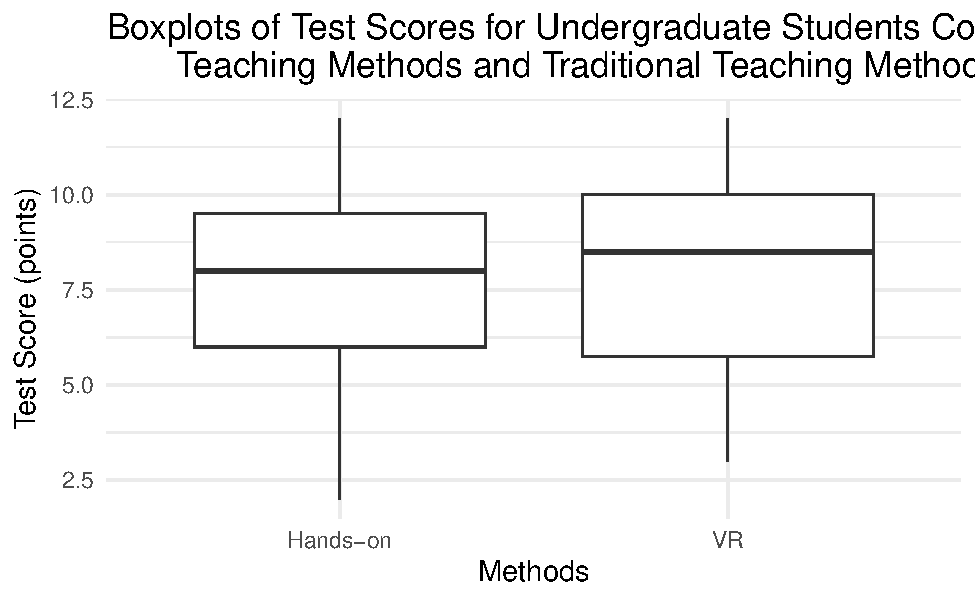
\includegraphics[width=0.7\linewidth]{12-A25-inference-1ofeach-theory_files/figure-latex/unnamed-chunk-1-1} \end{center}

\begin{Shaded}
\begin{Highlighting}[]
\NormalTok{moon }\SpecialCharTok{\%\textgreater{}\%}
  \FunctionTok{reframe}\NormalTok{(}\FunctionTok{favstats}\NormalTok{(TestScore}\SpecialCharTok{\textasciitilde{}}\NormalTok{Method))}
\end{Highlighting}
\end{Shaded}

\begin{verbatim}
#>     Method min   Q1 median   Q3 max     mean       sd  n missing
#> 1 Hands-on   2 6.00    8.0  9.5  12 7.694915 2.647408 59       0
#> 2       VR   3 5.75    8.5 10.0  12 7.982143 2.370202 56       0
\end{verbatim}

\begin{enumerate}
\def\labelenumi{\arabic{enumi}.}
\setcounter{enumi}{3}
\tightlist
\item
  Can theory-based methods be used to analyze these data?
\end{enumerate}

\vspace{1.2in}

\begin{enumerate}
\def\labelenumi{\arabic{enumi}.}
\setcounter{enumi}{4}
\tightlist
\item
  Calculate the summary statistic (difference in means) for this study. Use appropriate notation with clearly defined subscripts.
\end{enumerate}

\vspace{1in}

\subsubsection*{Use statistical inferential methods to draw inferences from the data}\label{use-statistical-inferential-methods-to-draw-inferences-from-the-data-4}
\addcontentsline{toc}{subsubsection}{Use statistical inferential methods to draw inferences from the data}

To find the standardized statistic for the difference in means we will calculate:

\[T = \frac{\bar{x}_1-\bar{x}_2 -0}{SE(\bar{x}_1-\bar{x}_2)},\]

where the standard error of the difference in means is calculated using:

\[SE(\bar{x}_1 -\bar{x}_2)=\sqrt{\frac{s_1^2}{n_1}+\frac{s_2^2}{n_2}}.\]

\begin{enumerate}
\def\labelenumi{\arabic{enumi}.}
\setcounter{enumi}{5}
\tightlist
\item
  Calculate the standard error for the difference in sample means.
\end{enumerate}

\vspace{0.5in}

\begin{enumerate}
\def\labelenumi{\arabic{enumi}.}
\setcounter{enumi}{6}
\tightlist
\item
  Calculate the standardized statistic for the difference in sample means.
\end{enumerate}

\vspace{0.5in}

To find the degrees of freedom to use for the t-distribution, we need to use the group with the smallest sample size and subtract 1. (\texttt{df} = minimum of \(n_1 - 1\) or \(n_2 - 1\)).

\vspace{0.2in}

\begin{itemize}
\item
  Enter the value of the standardized statistic for xx
\item
  Enter the df for yy
\end{itemize}

\begin{Shaded}
\begin{Highlighting}[]
\DecValTok{2}\SpecialCharTok{*}\FunctionTok{pt}\NormalTok{(xx, }\AttributeTok{df=}\NormalTok{yy, }\AttributeTok{lower.tail=}\ConstantTok{FALSE}\NormalTok{)}
\end{Highlighting}
\end{Shaded}

\vspace{0.3in}

\begin{enumerate}
\def\labelenumi{\arabic{enumi}.}
\setcounter{enumi}{7}
\tightlist
\item
  What is the p-value for the study?
\end{enumerate}

\vspace{0.2in}

To calculate a theory-based 95\% confidence interval for a difference in means, use the formula:

\[(\bar{x}_1- \bar{x}_2)\pm (t^* \times SE(\bar{x}_1- \bar{x}_2))\]

We will need to find the \(t^*\) multiplier using the function \texttt{qt()}. For a 95\% confidence level, we are finding the \(t^*\) value at the 97.5th percentile with (\texttt{df} = minimum of \(n_1 - 1\) or \(n_2 - 1\)).

\begin{Shaded}
\begin{Highlighting}[]
\FunctionTok{qt}\NormalTok{(}\FloatTok{0.975}\NormalTok{, }\AttributeTok{df =} \DecValTok{55}\NormalTok{, }\AttributeTok{lower.tail=}\ConstantTok{TRUE}\NormalTok{)}
\end{Highlighting}
\end{Shaded}

\begin{verbatim}
#> [1] 2.004045
\end{verbatim}

\begin{enumerate}
\def\labelenumi{\arabic{enumi}.}
\setcounter{enumi}{8}
\tightlist
\item
  Calculate the 95\% confidence interval using theory-based methods.
\end{enumerate}

\vspace{0.5in}

\begin{enumerate}
\def\labelenumi{\arabic{enumi}.}
\setcounter{enumi}{9}
\tightlist
\item
  Write a conclusion to the test.
  \vspace{0.7in}
\end{enumerate}

\subsection{Take-home messages}\label{take-home-messages-4}

\begin{enumerate}
\def\labelenumi{\arabic{enumi}.}
\item
  In order to use theory-based methods for independent groups, the normality condition must be met for each sample.
\item
  A T-score is compared to a \(t\)-distribution with the minimum \(n - 1\) df in order to calculate a one-sided p-value. To find a two-sided p-value using theory-based methods we need to multiply the one-sided p-value by 2.
\item
  A \(t^*\) multiplier is found by obtaining the bounds of the middle X\% (X being the desired confidence level) of a \(t\)-distribution with the minimum \(n - 1\) df.
\end{enumerate}

\subsection{Additional notes}\label{additional-notes-4}

Use this space to summarize your thoughts and take additional notes on today's activity and material covered

\vspace{3in}
\newpage

\section{Module 12 Lab: Trustworthiness}\label{module-12-lab-trustworthiness}

\setstretch{1}

\subsection{Learning outcomes}\label{learning-outcomes-6}

\begin{itemize}
\item
  Given a research question involving one categorical explanatory variable and one quantitative response variable, construct the null and alternative hypotheses
  in words and using appropriate statistical symbols.
\item
  Describe and perform a theory-based hypothesis test for a difference in means.
\item
  Interpret and evaluate a p-value for a theory-based hypothesis test for a difference in means.
\item
  Use theory-based methods to find a confidence interval for a difference in means.
\item
  Interpret a confidence interval for a difference in means.
\item
  Use a confidence interval to determine the conclusion of a hypothesis test.
\end{itemize}

\subsection{Trustworthiness}\label{trustworthiness}

Researchers in India wanted to find out how trustworthy famous YouTubers are (Kalra 2022). They went through a process in which they collected data on many videos from famous YouTubers to determine a trustworthiness score. Scientists randomly selected videos from famous YouTubers (\textgreater1000 subscribers) to include in the study. There were many different factors that went into calculating the trustworthiness score. Researchers also recorded if YouTubers were a subject matter expert (SME) or not a subject matter expert (non-SME). An example of an SME would be if one of your statistics professors made a YouTube video of how to do hypothesis testing. An example of someone who isn't an SME would be if one of your friends who has never taken a civil engineering class in their life decided to make a YouTube video about how to build a bridge. There were 621 Youtubers who are SMEs in the sample and 1026 who aren't SMEs. Is there evidence of a difference in mean trustworthiness score between subject matter experts (SME) YouTubers and non-SME YouTubers? Use SME -- Non -SME as the order of subtraction

\begin{enumerate}
\def\labelenumi{\arabic{enumi}.}
\tightlist
\item
  \textbf{Write out the parameter of interest in words in context of the study.}
\end{enumerate}

\vspace{0.8in}

\begin{enumerate}
\def\labelenumi{\arabic{enumi}.}
\setcounter{enumi}{1}
\tightlist
\item
  Write out the null hypothesis in notation for this study. Be sure to clearly identify the subscripts.
\end{enumerate}

\vspace{0.5in}

\begin{enumerate}
\def\labelenumi{\arabic{enumi}.}
\setcounter{enumi}{2}
\tightlist
\item
  Write out the alternative hypothesis in words for this study.
\end{enumerate}

\vspace{0.8in}

The sampling distribution for \(\bar{x}_1-\bar{x}_2\) can be modeled using a normal distribution when certain conditions are met.

Conditions for the sampling distribution of \(\bar{x}_1-\bar{x}_2\) to follow an approximate normal distribution:

\begin{itemize}
\item
  \textbf{Independence}: The sample's observations are independent
\item
  \textbf{Normality}: Each sample should be approximately normal or have a large sample size. For \emph{each} sample:

  \begin{itemize}
  \item
    \(n < 30\): If the sample size \(n\) is less than 30 and there are no clear outliers in the data, then we typically assume the data come from a nearly normal distribution to satisfy the condition.
  \item
    \(30 \le n < 100\): If the sample size \(n\) is between 30 and 100 and there are no particularly extreme outliers, then we typically assume the sampling distribution of \(\bar{x}\) is nearly normal, even if the underlying distribution of individual observations is not.
  \item
    \(n \geq 100\): If the sample size \(n\) is at least 100 (regardless of the presence of skew or outliers), we typically assume the sampling distribution of \(\bar{x}\) is nearly normal, even if the underlying distribution of individual observations is not.
  \end{itemize}
\item
  Upload and open the R script file for Module 10 lab. Upload the csv file, \texttt{Trustworthiness.csv}.
\item
  Enter the name of the data set for datasetname in the R script file in line 10.
\item
  Write a title for the boxplots in line 14.
\item
  Highlight and run lines 1--16 to load the data and create plots of the data.
\end{itemize}

\begin{Shaded}
\begin{Highlighting}[]
\NormalTok{trust }\OtherTok{\textless{}{-}} \FunctionTok{read.csv}\NormalTok{(}\StringTok{"datasetname"}\NormalTok{)}
\NormalTok{trust }\SpecialCharTok{\%\textgreater{}\%}  \CommentTok{\# Data set piped into...}
  \FunctionTok{ggplot}\NormalTok{(}\FunctionTok{aes}\NormalTok{(}\AttributeTok{y =}\NormalTok{ Trustworthiness\_Video, }\AttributeTok{x =}\NormalTok{ Creator\_SME))}\SpecialCharTok{+}  \CommentTok{\# Identify variables}
  \FunctionTok{geom\_boxplot}\NormalTok{()}\SpecialCharTok{+}  \CommentTok{\# Tell it to make a box plot}
  \FunctionTok{labs}\NormalTok{(}\AttributeTok{title =} \StringTok{"Don\textquotesingle{}t forget to include a title"}\NormalTok{,  }\CommentTok{\# Title: should include the type of plot,}
       \CommentTok{\# observational units, variables}
       \AttributeTok{x =} \StringTok{"Whether the Creator is SME"}\NormalTok{,    }\CommentTok{\# x{-}axis label}
       \AttributeTok{y =} \StringTok{"Trustworthiness Score"}\NormalTok{)  }\CommentTok{\# y{-}axis label}
\end{Highlighting}
\end{Shaded}

\begin{enumerate}
\def\labelenumi{\arabic{enumi}.}
\setcounter{enumi}{3}
\item
  Is the independence condition met? Explain your answer.
  \vspace{0.8in}
\item
  Check that the normality condition is met to use theory-based methods to analyze these data.
\end{enumerate}

\vspace{0.8in}

\begin{itemize}
\item
  Enter the name of the explanatory variable for \texttt{explanatory} and the name of the response variable for \texttt{response} in line 22.
\item
  Highlight and run lines 21--22 to get the summary statistics for the data.
\end{itemize}

\begin{Shaded}
\begin{Highlighting}[]
\NormalTok{trust }\SpecialCharTok{\%\textgreater{}\%}
  \FunctionTok{reframe}\NormalTok{(}\FunctionTok{favstats}\NormalTok{(response}\SpecialCharTok{\textasciitilde{}}\NormalTok{explantory))}
\end{Highlighting}
\end{Shaded}

\begin{enumerate}
\def\labelenumi{\arabic{enumi}.}
\setcounter{enumi}{5}
\tightlist
\item
  \textbf{Calculate the summary measure (difference in means) for this study. Use appropriate notation with clearly defined subscripts.}
\end{enumerate}

\vspace{1in}

\subsubsection*{Use statistical inferential methods to draw inferences from the data}\label{use-statistical-inferential-methods-to-draw-inferences-from-the-data-5}
\addcontentsline{toc}{subsubsection}{Use statistical inferential methods to draw inferences from the data}

To find the standardized statistic for the difference in means we will calculate:

\[T = \frac{\bar{x}_1-\bar{x}_2 -0}{SE(\bar{x}_1-\bar{x}_2)},\]

where the standard error of the difference in means is calculated using:

\[SE(\bar{x}_1 -\bar{x}_2)=\sqrt{\frac{s_1^2}{n_1}+\frac{s_2^2}{n_2}}.\]

\begin{enumerate}
\def\labelenumi{\arabic{enumi}.}
\setcounter{enumi}{6}
\tightlist
\item
  Calculate the standard error for the difference in sample means.
\end{enumerate}

\vspace{0.5in}

\begin{enumerate}
\def\labelenumi{\arabic{enumi}.}
\setcounter{enumi}{7}
\tightlist
\item
  \textbf{Calculate the standardized statistic for the difference in sample means.}
\end{enumerate}

\vspace{0.5in}

\begin{enumerate}
\def\labelenumi{\arabic{enumi}.}
\setcounter{enumi}{8}
\tightlist
\item
  When we are comparing two quantitative variables to find the degrees of freedom to use for the t-distribution, we need to use the group with the smallest sample size and subtract 1. (\texttt{df} = minimum of \(n_1 - 1\) or \(n_2 - 1\)). Calculate the \texttt{df} for this study.
\end{enumerate}

\vspace{0.2in}

\begin{enumerate}
\def\labelenumi{\arabic{enumi}.}
\setcounter{enumi}{9}
\tightlist
\item
  Using the provided R script file, enter the T-score (for \texttt{xx}) and the \texttt{df} calculated in question 9 for \texttt{yy} into the \texttt{pt()} function to find the p-value. Highlight and run line 27. Report the p-value calculated.
\end{enumerate}

\begin{Shaded}
\begin{Highlighting}[]
\DecValTok{2}\SpecialCharTok{*}\FunctionTok{pt}\NormalTok{(xx, }\AttributeTok{df=}\NormalTok{yy, }\AttributeTok{lower.tail=}\ConstantTok{FALSE}\NormalTok{)}
\end{Highlighting}
\end{Shaded}

\vspace{0.2in}

\begin{enumerate}
\def\labelenumi{\arabic{enumi}.}
\setcounter{enumi}{10}
\item
  \textbf{Explain why we multiplied by 2 in the code above.}
  \vspace{0.3in}
\item
  Do you expect the 95\% confidence interval to contain the null value of zero? Explain your answer.
  \vspace{0.8in}
\end{enumerate}

To calculate a theory-based 95\% confidence interval for a difference in means, use the formula:

\[(\bar{x}_1- \bar{x}_2)\pm (t^* \times SE(\bar{x}_1- \bar{x}_2))\]

We will need to find the \(t^*\) multiplier using the function \texttt{qt()}. For a 95\% confidence level, we are finding the \(t^*\) value at the 97.5th percentile with (\texttt{df} = minimum of \(n_1 - 1\) or \(n_2 - 1\)).

\begin{itemize}
\tightlist
\item
  Enter the appropriate percentile value (as a decimal) for \texttt{xx} and degrees of freedom for \texttt{yy} into the \texttt{qt()} function at line 32 to find the appropriate \(t^*\) multiplier
\end{itemize}

\begin{Shaded}
\begin{Highlighting}[]
\FunctionTok{qt}\NormalTok{(xx, }\AttributeTok{df =}\NormalTok{ yy, }\AttributeTok{lower.tail=}\ConstantTok{FALSE}\NormalTok{)}
\end{Highlighting}
\end{Shaded}

\begin{enumerate}
\def\labelenumi{\arabic{enumi}.}
\setcounter{enumi}{12}
\tightlist
\item
  Report the \(t^*\) multiplier for the 95\% confidence interval.
\end{enumerate}

\vspace{0.3in}

\begin{enumerate}
\def\labelenumi{\arabic{enumi}.}
\setcounter{enumi}{13}
\tightlist
\item
  Calculate the 95\% confidence interval using theory-based methods.
\end{enumerate}

\vspace{0.5in}

\begin{enumerate}
\def\labelenumi{\arabic{enumi}.}
\setcounter{enumi}{14}
\tightlist
\item
  Do the results of the CI agree with the p-value? Explain your answer.
\end{enumerate}

\vspace{0.5in}

\begin{enumerate}
\def\labelenumi{\arabic{enumi}.}
\setcounter{enumi}{15}
\item
  What type of error may be possible?
  \vspace{0.2in}
\item
  Write a paragraph summarizing the results of the study as if you are reporting the results to your supervisor. \textbf{Upload a copy of your paragraph to Gradescope for your group.} Be sure to describe:
\end{enumerate}

\begin{itemize}
\item
  Summary statistic and interpretation
\item
  P-value and interpretation

  \begin{itemize}
  \item
    Statement about probability or proportion of samples
  \item
    Statistic (summary measure and value)
  \item
    Direction of the alternative
  \item
    Null hypothesis (in context)
  \end{itemize}
\item
  Confidence interval and interpretation

  \begin{itemize}
  \item
    How confident you are (e.g., 90\%, 95\%, 98\%, 99\%)
  \item
    Parameter of interest
  \item
    Calculated interval
  \item
    Order of subtraction when comparing two groups
  \end{itemize}
\item
  Conclusion (written to answer the research question)

  \begin{itemize}
  \item
    Amount of evidence
  \item
    Parameter of interest
  \item
    Direction of the alternative hypothesis
  \end{itemize}
\item
  Scope of inference
\end{itemize}

\newpage

Paragraph continued:

\newpage

\chapter{Inference for Two Quantitative Variables}\label{inference-for-two-quantitative-variables}

\section{Vocabulary Review and Key Topics}\label{vocabulary-review-and-key-topics-2}

Review the Golden Ticket posted in the resources at the end of the coursepack for a summary of a two quantitative variables.

Types of plot for two quantitative variables

\begin{itemize}
\item
  \textbf{Scatterplot}: plots (x,y) pairs of observations
\item
  Four characteristics of scatterplots

  \begin{itemize}
  \item
    Form (linear or non-linear)
  \item
    Direction (positive or negative)
  \item
    Strength (weak, moderate, or strong)
  \item
    Outliers?
  \end{itemize}
\end{itemize}

R code to create a scatterplot:

\begin{Shaded}
\begin{Highlighting}[]
\NormalTok{object }\SpecialCharTok{\%\textgreater{}\%} \CommentTok{\# Pipe data set into...}
\FunctionTok{ggplot}\NormalTok{(}\FunctionTok{aes}\NormalTok{(}\AttributeTok{x =}\NormalTok{ explanatory, }\AttributeTok{y =}\NormalTok{ response))}\SpecialCharTok{+}  \CommentTok{\# Specify variables}
  \FunctionTok{geom\_point}\NormalTok{(}\AttributeTok{alpha=}\FloatTok{0.5}\NormalTok{) }\SpecialCharTok{+}  \CommentTok{\# Add scatterplot of points}
  \FunctionTok{labs}\NormalTok{(}\AttributeTok{x =} \StringTok{"x{-}axis label"}\NormalTok{,  }\CommentTok{\# Label x{-}axis}
       \AttributeTok{y =} \StringTok{"y{-}axis lable"}\NormalTok{,  }\CommentTok{\# Label y{-}axis}
       \AttributeTok{title =} \StringTok{"Don\textquotesingle{}t forget to add a title!"}\NormalTok{) }\SpecialCharTok{+} 
               \CommentTok{\# Be sure to tile your plots}
  \FunctionTok{geom\_smooth}\NormalTok{(}\AttributeTok{method =} \StringTok{"lm"}\NormalTok{, }\AttributeTok{se =} \ConstantTok{FALSE}\NormalTok{)  }\CommentTok{\# Add regression line}
\end{Highlighting}
\end{Shaded}

Summary measures

\begin{itemize}
\tightlist
\item
  \textbf{Slope of the regression line}: measures the magnitude and direction of the linear relationship between two quantitative variables
\end{itemize}

\[\widehat{response} = b_0 + b_1 \times explanatory\]
\vspace{1mm}

\begin{itemize}
\item
  Parameter notation for slope: \(\beta_1\)
\item
  Sample notation for slope: \(b_1\)
\item
  R code to create the linear model
\end{itemize}

\begin{Shaded}
\begin{Highlighting}[]
\NormalTok{linearmodel }\OtherTok{\textless{}{-}} \FunctionTok{lm}\NormalTok{(response}\SpecialCharTok{\textasciitilde{}}\NormalTok{explanatory, }\AttributeTok{data=}\NormalTok{object)}
\FunctionTok{round}\NormalTok{(}\FunctionTok{summary}\NormalTok{(linearmodel)}\SpecialCharTok{$}\NormalTok{coefficients,}\DecValTok{3}\NormalTok{) }\CommentTok{\# Display coefficient}
\end{Highlighting}
\end{Shaded}

\begin{itemize}
\item
  \textbf{Correlation}: measures the strength and direction of the linear relationship between two quantitative variables

  \begin{itemize}
  \item
    Parameter notation: \(\rho\)
  \item
    Sample notation: \(r\)
  \end{itemize}
\item
  \textbf{Coefficient of determination}: measures the percent of total variability in the response variable that is explained by the relationship with the explanatory variable
\end{itemize}

\[r^2 = (r)^2 = \frac{SST - SSE}{SST} = \frac{s^2_y - s^2_{residual}}{s^2_y}\]

\subsection*{Simulation Hypothesis Testing}\label{simulation-hypothesis-testing-2}
\addcontentsline{toc}{subsection}{Simulation Hypothesis Testing}

\begin{itemize}
\tightlist
\item
  Can test either slope or correlation - both test for a linear relationship between two quantitative variables
\end{itemize}

Hypotheses for slope:

\[H_0: \beta_1 = 0\]

\[H_A: \beta_1 \left\{
\begin{array}{ll}
< \\
\ne \\
< \\
\end{array}
\right\}
0\]

Hypotheses for correlation:

\[H_0: \rho = 0\]
\[H_A: \rho \left\{
\begin{array}{ll}
< \\
\ne \\
< \\
\end{array}
\right\}
0\]

\begin{itemize}
\tightlist
\item
  R code for simulation methods to find the p-value using the \texttt{regression\_test} function in the \texttt{catstats} package.
\end{itemize}

\begin{Shaded}
\begin{Highlighting}[]
\FunctionTok{regression\_test}\NormalTok{(response}\SpecialCharTok{\textasciitilde{}}\NormalTok{explanatory, }\CommentTok{\# response \textasciitilde{} explanatory}
               \AttributeTok{data =}\NormalTok{ object, }\CommentTok{\# Name of data set}
               \AttributeTok{direction =} \StringTok{"xx"}\NormalTok{, }\CommentTok{\# Sign in alternative ("greater", "less", "two{-}sided")}
               \AttributeTok{summary\_measure =} \StringTok{"xx"}\NormalTok{, }\CommentTok{\# "slope" or "correlation"}
               \AttributeTok{as\_extreme\_as =}\NormalTok{ xx, }\CommentTok{\# Observed slope or correlation}
               \AttributeTok{number\_repetitions =} \DecValTok{10000}\NormalTok{) }\CommentTok{\# Number of simulated samples for null distribution}
\end{Highlighting}
\end{Shaded}

\subsection*{Conditions necessary to use theory-based methods}\label{conditions-necessary-to-use-theory-based-methods}
\addcontentsline{toc}{subsection}{Conditions necessary to use theory-based methods}

\subsection*{Theory-based Methods to find the p-value}\label{theory-based-methods-to-find-the-p-value}
\addcontentsline{toc}{subsection}{Theory-based Methods to find the p-value}

\begin{itemize}
\tightlist
\item
  To find the value of the standardized statistic to test the slope we will use,
\end{itemize}

\[
T = \frac{\mbox{slope estimate}-null value}{SE} = \frac{b_1-0}{SE(b_1)}.
\]
* Use the standard error estimate from the linear model output

\begin{itemize}
\item
  The p-value can be found from the linear model output or by using the pt function.

  \begin{itemize}
  \item
    Enter the value of the standardized statistic for xx
  \item
    Enter the df \((n-2)\) for yy
  \end{itemize}
\end{itemize}

\begin{Shaded}
\begin{Highlighting}[]
\FunctionTok{pt}\NormalTok{(xx, }\AttributeTok{df =}\NormalTok{ yy, }\AttributeTok{lower.tail=}\ConstantTok{TRUE}\NormalTok{)}
\end{Highlighting}
\end{Shaded}

\subsection*{Simulation methods to find the confidence interval}\label{simulation-methods-to-find-the-confidence-interval}
\addcontentsline{toc}{subsection}{Simulation methods to find the confidence interval}

\begin{itemize}
\tightlist
\item
  R code to find the simulation confidence interval using the \texttt{regression\_bootstrap\_CI} function from the \texttt{catstats} package.
\end{itemize}

\begin{Shaded}
\begin{Highlighting}[]
\FunctionTok{regression\_bootstrap\_CI}\NormalTok{(response}\SpecialCharTok{\textasciitilde{}}\NormalTok{explanatory, }\CommentTok{\# response \textasciitilde{} explanatory}
   \AttributeTok{data =}\NormalTok{ object, }\CommentTok{\# Name of data set}
   \AttributeTok{confidence\_level =}\NormalTok{ xx, }\CommentTok{\# Confidence level as decimal}
   \AttributeTok{summary\_measure =} \StringTok{"xx"}\NormalTok{, }\CommentTok{\# Slope or correlation}
   \AttributeTok{number\_repetitions =} \DecValTok{10000}\NormalTok{) }\CommentTok{\# Number of simulated samples for bootstrap distribution}
\end{Highlighting}
\end{Shaded}

\subsection*{Theory-based methods to find the confidence interval}\label{theory-based-methods-to-find-the-confidence-interval}
\addcontentsline{toc}{subsection}{Theory-based methods to find the confidence interval}

\begin{itemize}
\item
  R code to find the multiplier for the confidence interval using theory-based methods.

  \begin{itemize}
  \item
    pt will give you a p-value using the t-distribution with n-2 df (enter for yy)
  \item
    Enter the value of the standardized statistic for xx
  \item
    If a greater than alternative, change lower.tail = TRUE to FALSE.
  \item
    If a two-sided test, multiply by 2.
  \end{itemize}
\end{itemize}

\begin{Shaded}
\begin{Highlighting}[]
\FunctionTok{pt}\NormalTok{(xx, }\AttributeTok{df=}\NormalTok{yy, }\AttributeTok{lower.tail=}\ConstantTok{FALSE}\NormalTok{)}
\end{Highlighting}
\end{Shaded}

\newpage

\section{Video Notes: Regression and Correlation}\label{video-notes-regression-and-correlation}

Read Chapters 6, 7, and 8 in the course textbook. Use the following videos to complete the video notes for Module 13.

\subsection{Course Videos}\label{course-videos-2}

\begin{itemize}
\item
  6.1
\item
  6.2
\item
  6.3
\item
  Ch 7
\end{itemize}

\setstretch{1}

\subsection*{Summary measures and plots for two quantitative variables - Videos 6.1 - 6.3}\label{summary-measures-and-plots-for-two-quantitative-variables---videos-6.1---6.3}
\addcontentsline{toc}{subsection}{Summary measures and plots for two quantitative variables - Videos 6.1 - 6.3}

Example: Data were collected from 1236 births between 1960 and 1967 in the San Francisco East Bay area to better understand what variables contributed to child birthweight, as children with low birthweight often suffer from an array of complications later in life ({``Child Health and Development Studies,''} n.d.). There were some missing values in the study and with those observations removed we have a total of 1223 births.

\begin{Shaded}
\begin{Highlighting}[]
\NormalTok{babies}\OtherTok{\textless{}{-}}\FunctionTok{read.csv}\NormalTok{(}\StringTok{"data/babies.csv"}\NormalTok{) }\SpecialCharTok{\%\textgreater{}\%}
    \FunctionTok{drop\_na}\NormalTok{(bwt) }\SpecialCharTok{\%\textgreater{}\%}
    \FunctionTok{drop\_na}\NormalTok{(gestation)}
\FunctionTok{glimpse}\NormalTok{(babies)}
\CommentTok{\#\textgreater{} Rows: 1,223}
\CommentTok{\#\textgreater{} Columns: 8}
\CommentTok{\#\textgreater{} $ case      \textless{}int\textgreater{} 1, 2, 3, 5, 6, 7, 8, 9, 10, 11, 12, 13, 14, 15, 16, 17, 18, \textasciitilde{}}
\CommentTok{\#\textgreater{} $ bwt       \textless{}int\textgreater{} 120, 113, 128, 108, 136, 138, 132, 120, 143, 140, 144, 141, \textasciitilde{}}
\CommentTok{\#\textgreater{} $ gestation \textless{}int\textgreater{} 284, 282, 279, 282, 286, 244, 245, 289, 299, 351, 282, 279, \textasciitilde{}}
\CommentTok{\#\textgreater{} $ parity    \textless{}int\textgreater{} 0, 0, 0, 0, 0, 0, 0, 0, 0, 0, 0, 0, 0, 0, 0, 0, 0, 0, 0, 0, \textasciitilde{}}
\CommentTok{\#\textgreater{} $ age       \textless{}int\textgreater{} 27, 33, 28, 23, 25, 33, 23, 25, 30, 27, 32, 23, 36, 30, 38, \textasciitilde{}}
\CommentTok{\#\textgreater{} $ height    \textless{}int\textgreater{} 62, 64, 64, 67, 62, 62, 65, 62, 66, 68, 64, 63, 61, 63, 63, \textasciitilde{}}
\CommentTok{\#\textgreater{} $ weight    \textless{}int\textgreater{} 100, 135, 115, 125, 93, 178, 140, 125, 136, 120, 124, 128, 9\textasciitilde{}}
\CommentTok{\#\textgreater{} $ smoke     \textless{}int\textgreater{} 0, 0, 1, 1, 0, 0, 0, 0, 1, 0, 1, 1, 1, 0, 0, 1, 1, 0, 1, 0, \textasciitilde{}}
\end{Highlighting}
\end{Shaded}

Here you see a glimpse of the data. The 1223 rows correspond to the sample size. The case variable is labeling each pregnancy 1 through 1223. Then 7 variables are recorded. birthweight (bwt), length of gestation in days, parity is called an indicator variable telling us if the pregnancy was a first pregnancy (labeled as 0) or not (labeled as 1) were recorded about the child and pregnancy. The age, height, and weight were recorded for the mother giving birth, as was smoke, another indicator variable where 0 means the mother did not smoke during pregnancy, and 1 indicates that she did smoke while pregnant.

\setstretch{1.5}

\subsubsection*{Type of plot}\label{type-of-plot}
\addcontentsline{toc}{subsubsection}{Type of plot}

A \_\_\_\_\_\_\_\_\_\_\_\_\_\_\_\_\_\_ is used to display the relationship
between two \_\_\_\_\_\_\_\_\_\_\_\_\_\_\_\_\_\_\_ variables.

\setstretch{1}
\newpage

Four characteristics of the scatterplot:

\begin{itemize}
\tightlist
\item
  Form:
\end{itemize}

\vspace{0.2in}

\begin{itemize}
\tightlist
\item
  Direction:
\end{itemize}

\vspace{0.2in}

\begin{itemize}
\tightlist
\item
  Strength:
\end{itemize}

\vspace{0.2in}

\begin{itemize}
\tightlist
\item
  Outliers:
\end{itemize}

\vspace{0.2in}

\rgi \rgi - Influential points: outliers that change the regression line; far from the line of regression

\rgi \rgi - High leverage points: outliers that are extreme in the x- axis; far from the mean of the x-axis

The following shows a scatterplot of length of gestation as a predictor of birthweight.

\begin{Shaded}
\begin{Highlighting}[]
\NormalTok{babies }\SpecialCharTok{\%\textgreater{}\%} \CommentTok{\# Data set pipes into...}
\FunctionTok{ggplot}\NormalTok{(}\FunctionTok{aes}\NormalTok{(}\AttributeTok{x =}\NormalTok{ gestation, }\AttributeTok{y =}\NormalTok{ bwt))}\SpecialCharTok{+}  \CommentTok{\# Specify variables}
  \FunctionTok{geom\_point}\NormalTok{(}\AttributeTok{alpha=}\FloatTok{0.5}\NormalTok{) }\SpecialCharTok{+}  \CommentTok{\# Add scatterplot of points}
  \FunctionTok{labs}\NormalTok{(}\AttributeTok{x =} \StringTok{"number of days of gestation"}\NormalTok{,  }\CommentTok{\# Label x{-}axis}
       \AttributeTok{y =} \StringTok{"birthweight (oz)"}\NormalTok{,  }\CommentTok{\# Label y{-}axis}
       \AttributeTok{title =} \StringTok{"Scatterplot of Gestation vs. Birthweight for Births}
\StringTok{       between 1960 and 1967 in San Francisco"}\NormalTok{) }\SpecialCharTok{+} 
    \CommentTok{\# Be sure to title your plots with the type of plot, observational units, variable(s)}
  \FunctionTok{geom\_smooth}\NormalTok{(}\AttributeTok{method =} \StringTok{"lm"}\NormalTok{, }\AttributeTok{se =} \ConstantTok{FALSE}\NormalTok{) }\SpecialCharTok{+} \CommentTok{\# Add regression line}
    \FunctionTok{theme\_bw}\NormalTok{()}
\end{Highlighting}
\end{Shaded}

\begin{center}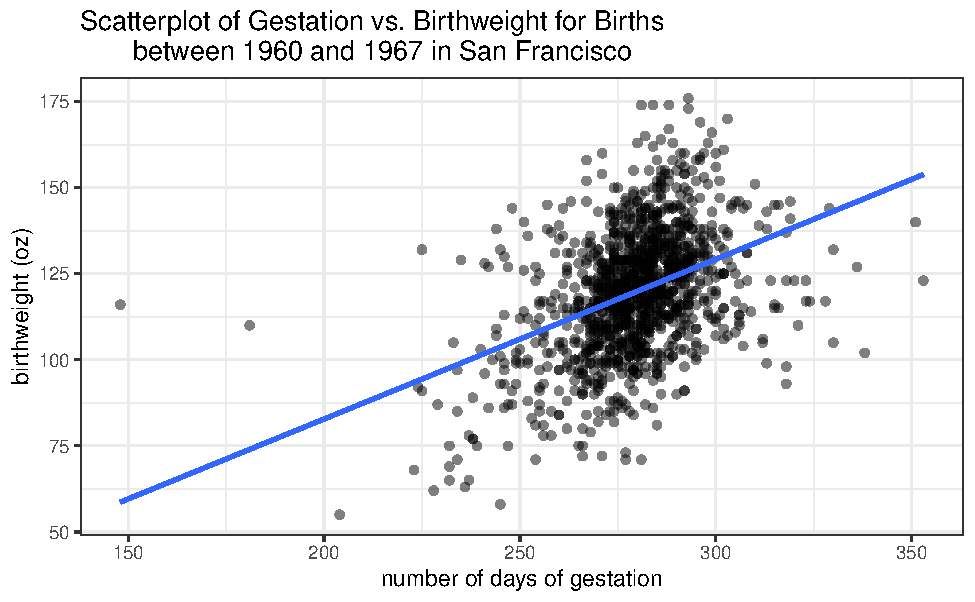
\includegraphics[width=0.8\linewidth]{13-VN13-regression_files/figure-latex/unnamed-chunk-2-1} \end{center}

Describe the scatterplot using the four characteristics of a scatterplot.

\vspace{1in}

\setstretch{1.5}

The summary measures for two quantitative variables are:

\begin{itemize}
\item
  \begin{center}\rule{0.5\linewidth}{0.5pt}\end{center}
\item
  \begin{center}\rule{0.5\linewidth}{0.5pt}\end{center}
\item
  \begin{center}\rule{0.5\linewidth}{0.5pt}\end{center}
\end{itemize}

\setstretch{1}

Notation:

\begin{itemize}
\item
  Population slope:
\item
  Population correlation:
\item
  Sample slope:
\item
  Sample correlation:
\end{itemize}

\subsubsection*{Correlation}\label{correlation}
\addcontentsline{toc}{subsubsection}{Correlation}

Correlation is always between the values of \_\_\_\_\_\_\_ and \_\_\_\_\_\_\_\_.

\begin{itemize}
\item
  Measures the \_\_\_\_\_\_\_\_\_\_\_\_\_ and \_\_\_\_\_\_\_\_\_\_\_\_\_\_ of the linear relationship between two quantitative variables.
\item
  The stronger the relationship between the variables the closer the value of \_\_\_\_\_\_\_\_\_\_\_\_\_\_\_ is to \_\_\_\_\_\_\_\_ or \_\_\_\_\_\_\_\_.
\item
  The sign gives the \_\_\_\_\_\_\_\_\_\_\_\_\_\_\_\_\_.
\end{itemize}

The following code creates a correlation matrix between different quantitative variables in the data set.

\begin{Shaded}
\begin{Highlighting}[]
\NormalTok{babies }\SpecialCharTok{\%\textgreater{}\%}
    \FunctionTok{select}\NormalTok{(}\FunctionTok{c}\NormalTok{(}\StringTok{"gestation"}\NormalTok{, }\StringTok{"age"}\NormalTok{, }\StringTok{"height"}\NormalTok{, }\StringTok{"weight"}\NormalTok{, }\StringTok{"bwt"}\NormalTok{)) }\SpecialCharTok{\%\textgreater{}\%}
    \FunctionTok{cor}\NormalTok{(}\AttributeTok{use=}\StringTok{"pairwise.complete.obs"}\NormalTok{) }\SpecialCharTok{\%\textgreater{}\%}
    \FunctionTok{round}\NormalTok{(}\DecValTok{3}\NormalTok{)}
\end{Highlighting}
\end{Shaded}

\begin{verbatim}
#>           gestation    age height weight   bwt
#> gestation     1.000 -0.056  0.064  0.022 0.408
#> age          -0.056  1.000 -0.005  0.147 0.029
#> height        0.064 -0.005  1.000  0.436 0.201
#> weight        0.022  0.147  0.436  1.000 0.154
#> bwt           0.408  0.029  0.201  0.154 1.000
\end{verbatim}

\setstretch{1.5}

The value of correlation between gestation and birthweight is \_\_\_\_\_\_\_\_\_\_\_\_\_\_. This shows a \_\_\_\_\_\_\_\_\_\_\_, \_\_\_\_\_\_\_\_\_\_\_\_\_ relationship between gestation and birthweight.

\setstretch{1}

\subsubsection*{Slope}\label{slope}
\addcontentsline{toc}{subsubsection}{Slope}

\begin{itemize}
\item
  Least-squares regression line: \(\hat{y}=b_0+b_1\times x\) (put y and x in the context of the problem) or \(\widehat{response}=b_0+b_1 \times \text{explanatory}\)
\item
  \(\hat{y}\) or \(\widehat{\text{response}}\) is
\end{itemize}

\vspace{0.1in}

\begin{itemize}
\tightlist
\item
  \(b_0\) is
\end{itemize}

\vspace{0.1in}

\begin{itemize}
\tightlist
\item
  \(b_1\) is
\end{itemize}

\vspace{0.1in}

\begin{itemize}
\tightlist
\item
  \(x\) or explanatory is
\end{itemize}

\vspace{0.1in}

\setstretch{1.5}

\begin{itemize}
\item
  The estimates for the linear model output will give the value of the \_\_\_\_\_\_\_\_\_\_\_\_\_\_\_\_\_\_\_ and the \_\_\_\_\_\_\_\_\_\_\_\_\_\_.
\item
  Interpretation of slope: an increase in the \_\_\_\_\_\_\_\_\_\_\_\_\_ variable of 1 unit is associated with an increase/decrease in the \_\_\_\_\_\_\_\_\_\_\_\_\_\_\_\_ variable by the value of slope, on average.
\item
  Interpretation of the y-intercept: for a value of 0 for the \_\_\_\_\_\_\_\_\_\_\_\_\_ variable, the predicted value for the \_\_\_\_\_\_\_\_\_\_ variable would be the value of y-intercept.
\item
  We can predict values of the \_\_\_\_\_\_\_\_\_\_\_ variable by plugging in a given \_\_\_\_\_\_\_\_\_\_ variable value using the least squares equation line.
\item
  A prediction of a response variable value for an explanatory value outside the range of x values is called \_\_\_\_\_\_\_\_\_\_\_\_\_\_\_.
\item
  To find how far the predicted value deviates from the actual value we find the \_\_\_\_\_\_\_\_\_\_\_\_.
\end{itemize}

\vspace{0.3in}

\begin{itemize}
\item
  To find the least squares regression line the line with the \_\_\_\_\_\_\_\_\_\_ SSE is found.

  SSE = sum of squared errors

  \begin{itemize}
  \tightlist
  \item
    To find SSE, the residual for each data point is found, squared and all the squared residuals are summed together
  \end{itemize}
\end{itemize}

The linear model output for this study is given below:

\begin{Shaded}
\begin{Highlighting}[]
\CommentTok{\# Fit linear model: y \textasciitilde{} x}
\NormalTok{babiesLM }\OtherTok{\textless{}{-}} \FunctionTok{lm}\NormalTok{(bwt }\SpecialCharTok{\textasciitilde{}}\NormalTok{ gestation, }\AttributeTok{data=}\NormalTok{babies)}
\FunctionTok{round}\NormalTok{(}\FunctionTok{summary}\NormalTok{(babiesLM)}\SpecialCharTok{$}\NormalTok{coefficients,}\DecValTok{3}\NormalTok{) }\CommentTok{\# Display coefficient summary}
\end{Highlighting}
\end{Shaded}

\begin{verbatim}
#>             Estimate Std. Error t value Pr(>|t|)
#> (Intercept)  -10.064      8.322  -1.209    0.227
#> gestation      0.464      0.030  15.609    0.000
\end{verbatim}

Write the least squares equation of the line.

\vspace{0.6in}

Interpret the slope in context of the problem.

\vspace{0.6in}

Interpret the y-intercept in context of the problem.

\vspace{0.6in}

Predict the birthweight for a birth with a baby born at 310 days gestation.

\vspace{0.5in}

Calculate the residual for a birth of a baby with a birthweight of 151 ounces and born at 310 days gestation.

\vspace{0.5in}

Is this value (310, 151) above or below the line of regression? Did the line of regression overestimate or underestimate the birthweight?

\vspace{0.2in}

\subsubsection*{Coefficient of Determination}\label{coefficient-of-determination}
\addcontentsline{toc}{subsubsection}{Coefficient of Determination}

The coefficient of determination can be found by squaring the value of correlation, using the variances for each variable or using the SSE (sum of squares error) and SST (sum of squares total)

\begin{itemize}
\item
  \(r^2 = (r)^2 = \frac{SST - SSE}{SST} = \frac{s^2_y - s^2_{residual}}{s^2_y}\)
\item
  The coefficient of determination measures the \_\_\_\_\_\_\_\_\_\_\_\_ of total variation in the \_\_\_\_\_\_\_\_\_\_\_ variable that is explained by the changes in the \_\_\_\_\_\_\_\_\_\_\_\_\_ variable.
\end{itemize}

\setstretch{1}

\begin{center}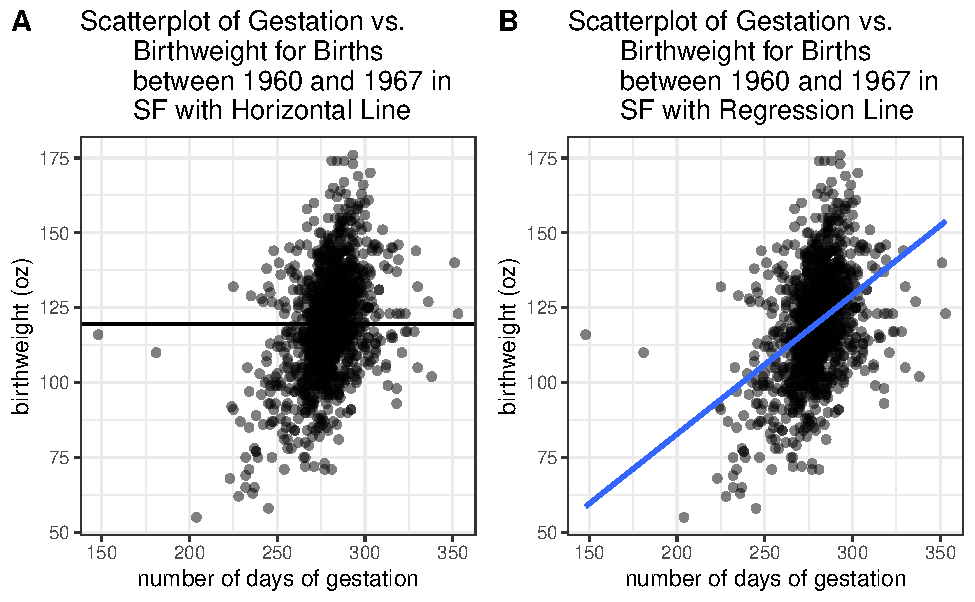
\includegraphics[width=0.7\linewidth]{13-VN13-regression_files/figure-latex/unnamed-chunk-6-1} \end{center}

The value for SST was calculated as 406753.48. The value for SSE was calculated as 339092.13.

Calculate the coefficient of determination between gestation and birthweight.

\vspace{0.3in}

Interpret the coefficient of determination between gestation and birthweight.

\vspace{0.5in}

\newpage

\subsubsection*{Multivariable plots - Video Chapter7}\label{multivariable-plots---video-chapter7}
\addcontentsline{toc}{subsubsection}{Multivariable plots - Video Chapter7}

Aesthetics: visual property of the objects in your plot

\setstretch{1.5}

\begin{itemize}
\item
  Position on the axes: groups for \_\_\_\_\_\_\_\_\_\_\_\_\_\_\_ variables, or a number line if the variable is \_\_\_\_\_\_\_\_\_\_\_\_\_\_\_\_\_
\item
  Color or shape - to represent \_\_\_\_\_\_\_\_\_\_\_\_\_\_\_ variables
\item
  Size - to represent \_\_\_\_\_\_\_\_\_\_\_\_\_\_\_\_ variables
\end{itemize}

\setstretch{1}

Adding the quantitative variable maternal age to the scatterplot between gestation and birthweight.

\begin{Shaded}
\begin{Highlighting}[]
\NormalTok{babies }\SpecialCharTok{\%\textgreater{}\%} \CommentTok{\# Data set pipes into...}
\FunctionTok{ggplot}\NormalTok{(}\FunctionTok{aes}\NormalTok{(}\AttributeTok{x =}\NormalTok{ gestation, }\AttributeTok{y =}\NormalTok{ bwt))}\SpecialCharTok{+}  \CommentTok{\# Specify variables}
  \FunctionTok{geom\_point}\NormalTok{(}\AttributeTok{alpha=}\FloatTok{0.5}\NormalTok{, }\AttributeTok{shape=}\DecValTok{1}\NormalTok{, }\FunctionTok{aes}\NormalTok{(}\AttributeTok{size=}\NormalTok{age)) }\SpecialCharTok{+}  \CommentTok{\# Add scatterplot of points}
  \FunctionTok{labs}\NormalTok{(}\AttributeTok{x =} \StringTok{"number of days of gestation"}\NormalTok{,  }\CommentTok{\# Label x{-}axis}
       \AttributeTok{y =} \StringTok{"birthweight (oz)"}\NormalTok{,  }\CommentTok{\# Label y{-}axis}
       \AttributeTok{title =} \StringTok{"Scatterplot of Gestation vs. Birthweight by Age }
\StringTok{       for Births between 1960 and 1967 in San Francisco"}\NormalTok{) }\SpecialCharTok{+} 
    \CommentTok{\# Be sure to title your plots}
  \FunctionTok{geom\_smooth}\NormalTok{(}\AttributeTok{method =} \StringTok{"lm"}\NormalTok{, }\AttributeTok{se =} \ConstantTok{FALSE}\NormalTok{)  }\CommentTok{\# Add regression line}
\end{Highlighting}
\end{Shaded}

\begin{center}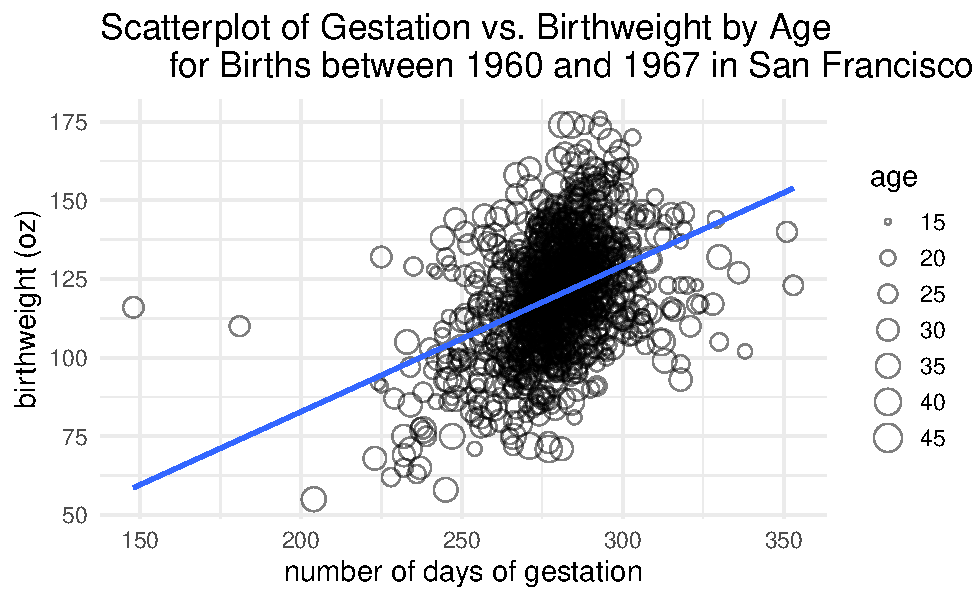
\includegraphics[width=0.8\linewidth]{13-VN13-regression_files/figure-latex/unnamed-chunk-7-1} \end{center}

\newpage

Let's add the categorical variable, whether a mother smoked, to the scatterplot between gestation and birthweight.

\begin{Shaded}
\begin{Highlighting}[]
\NormalTok{babies }\OtherTok{\textless{}{-}}\NormalTok{ babies }\SpecialCharTok{\%\textgreater{}\%} 
    \FunctionTok{mutate}\NormalTok{(}\AttributeTok{smoke =} \FunctionTok{factor}\NormalTok{(smoke)) }\SpecialCharTok{\%\textgreater{}\%}
    \FunctionTok{na.omit}\NormalTok{()}
           
\NormalTok{babies }\SpecialCharTok{\%\textgreater{}\%} \CommentTok{\# Data set pipes into...}
    \FunctionTok{ggplot}\NormalTok{(}\FunctionTok{aes}\NormalTok{(}\AttributeTok{x =}\NormalTok{ gestation, }\AttributeTok{y =}\NormalTok{ bwt, }\AttributeTok{color =}\NormalTok{ smoke))}\SpecialCharTok{+}  \CommentTok{\#Specify variables}
    \FunctionTok{geom\_point}\NormalTok{(}\FunctionTok{aes}\NormalTok{(}\AttributeTok{shape =}\NormalTok{ smoke), }\AttributeTok{size =} \DecValTok{2}\NormalTok{) }\SpecialCharTok{+}  \CommentTok{\#Add scatterplot of points}
    \FunctionTok{labs}\NormalTok{(}\AttributeTok{x =} \StringTok{"number of days of gestation"}\NormalTok{,  }\CommentTok{\#Label x{-}axis}
         \AttributeTok{y =} \StringTok{"birthweight (oz)"}\NormalTok{,  }\CommentTok{\#Label y{-}axis}
         \AttributeTok{title =} \StringTok{"Scatterplot of Gestation vs. Birthweight by }
\StringTok{         Smoking Status for Births between 1960 and 1967 }
\StringTok{         in San Francisco"}\NormalTok{) }\SpecialCharTok{+} 
    \CommentTok{\#Be sure to title your plots}
    \FunctionTok{geom\_smooth}\NormalTok{(}\AttributeTok{method =} \StringTok{"lm"}\NormalTok{, }\AttributeTok{se =} \ConstantTok{FALSE}\NormalTok{) }\SpecialCharTok{+} \CommentTok{\#Add regression line}
    \FunctionTok{scale\_color\_grey}\NormalTok{()}
\end{Highlighting}
\end{Shaded}

\begin{center}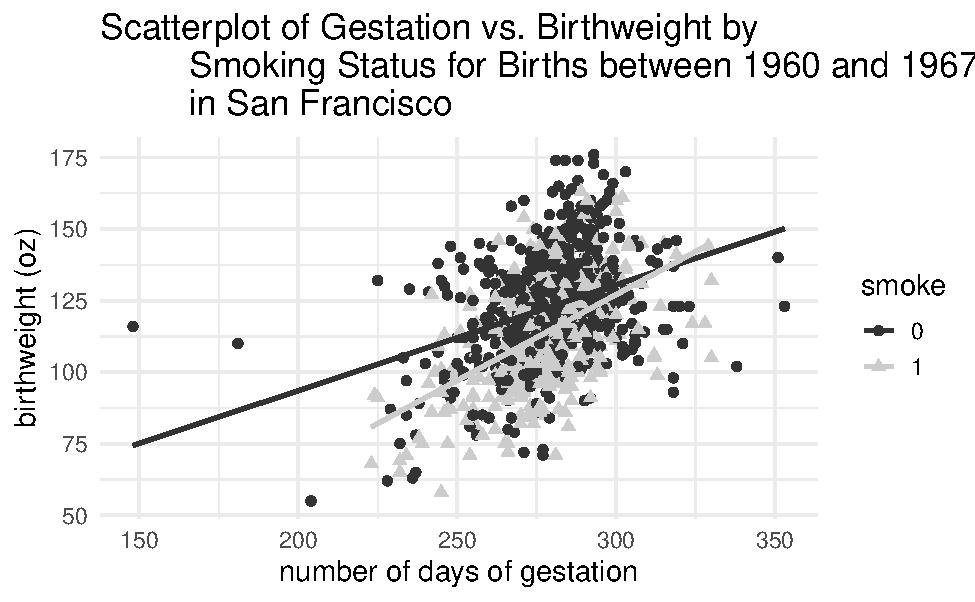
\includegraphics[width=0.8\linewidth]{13-VN13-regression_files/figure-latex/unnamed-chunk-8-1} \end{center}

Does the relationship between length of gestation and birthweight appear to depend upon maternal smoking status?

\vspace{1in}

Is the variable smoking status a potential confounding variable?

\vspace{1in}

Adding a categorical predictor:

\setstretch{1.5}

\begin{itemize}
\item
  Look at the regression line for each level of the \_\_\_\_\_\_\_\_\_\_\_\_\_\_
\item
  If the slopes are \_\_\_\_\_\_\_\_\_\_\_\_\_\_\_\_, the two predictor variables do not \_\_\_\_\_\_\_\_\_\_\_\_\_\_\_ to help explain the response
\item
  If the slopes \_\_\_\_\_\_\_\_\_\_\_\_\_\_\_\_\_, there is an interaction between the categorical predictor and the relationship between the two quantitative variables.
\end{itemize}

\setstretch{1}

\subsection{Concept Check}\label{concept-check-2}

Be prepared for group discussion in the next class. One member from the table should write the answers to the following on the whiteboard.

\begin{enumerate}
\def\labelenumi{\arabic{enumi}.}
\tightlist
\item
  What are the three summary measures for two quantitative variables?
\end{enumerate}

\vspace{0.5in}

\begin{enumerate}
\def\labelenumi{\arabic{enumi}.}
\setcounter{enumi}{1}
\tightlist
\item
  What are the four characteristics used to describe a scatterplot?
\end{enumerate}

\vspace{0.5in}

\begin{enumerate}
\def\labelenumi{\arabic{enumi}.}
\setcounter{enumi}{2}
\tightlist
\item
  When we add a categorical predictor variable to a scatterplot of two quantitative variables, what summary measure will we compare across the categories to assess the change in the relationship between the two quantitative variables.
\end{enumerate}

\vspace{0.2in}
\newpage

\subsection{Video Notes: Inference for Two Quantitative Variables}\label{video-notes-inference-for-two-quantitative-variables}

Read Chapters 21 and 22 in the course textbook. Use the following videos to complete the video notes for Module 11.

\subsection{Course Videos}\label{course-videos-3}

\begin{itemize}
\item
  21.1
\item
  21.3
\item
  21.4TheoryTests
\item
  21.4TheoryIntervals
\end{itemize}

\setstretch{1}

\subsection*{Summary measures and plots for two quantitative variables.}\label{summary-measures-and-plots-for-two-quantitative-variables.}
\addcontentsline{toc}{subsection}{Summary measures and plots for two quantitative variables.}

Scatterplot:

\begin{itemize}
\item
  Form: linear or non-linear?
\item
  Direction: positive or negative?
\item
  Strength: how clear is the pattern between the two variables?
\item
  Outliers: points that are far from the pattern or bulk of the data

  \begin{itemize}
  \tightlist
  \item
    Influential points: outliers that are extreme in the x-~variable.
  \end{itemize}
\end{itemize}

\setstretch{1.5}

The summary measures for two quantitative variables are:

\begin{itemize}
\tightlist
\item
  \_\_\_\_\_\_\_\_\_\_\_\_\_\_\_\_\_\_\_\_\_\_\_\_\_\_\_\_, interpreted as the on average change in the response variable for a one unit increase in the explanatory variable.
\end{itemize}

\vspace{1mm}

\begin{itemize}
\tightlist
\item
  \_\_\_\_\_\_\_\_\_\_\_\_\_\_\_\_\_\_\_\_\_\_\_\_\_\_\_\_, which measures the strength and direction of the linear relationship between two quantitative variables.
\end{itemize}

\vspace{1mm}

\begin{itemize}
\tightlist
\item
  \_\_\_\_\_\_\_\_\_\_\_\_\_\_\_\_\_\_\_\_\_\_\_\_\_\_\_\_, interpreted as the percent of variability in the response variable that is explained by the relationship with the explanatory variable.
\end{itemize}

\vspace{1mm}

\setstretch{1}

\begin{itemize}
\tightlist
\item
  Least-squares regression line: \(\hat{y}=b_0+b_1\times x\) (put y and x in the context of the problem)
\end{itemize}

\setstretch{1.5}

Notation:

\begin{itemize}
\item
  Population slope:
\item
  Population correlation:
\item
  Sample slope:
\item
  Sample correlation:
\end{itemize}

\setstretch{1}

Example: Oceanic temperature is important for sea life. The California Cooperative Oceanic Fisheries Investigations has measured several variables on the Pacific Ocean for more than 70 years hoping to better understand weather patterns and impacts on ocean life. ({``Ocean Temperature and Salinity Study,''} n.d.) For this example, we will look at the most recent 100 measurements of salt water salinity (measured in PSUs or practical salinity units) and the temperature of the ocean measured in degrees Celsius. Is there evidence that water temperature in the Pacific Ocean tends to decrease with higher levels of salinity?

\subsection*{Hypothesis Testing}\label{hypothesis-testing-2}
\addcontentsline{toc}{subsection}{Hypothesis Testing}

Null hypothesis assumes ``no effect'', ``no difference'', ``nothing interesting happening'', etc.

\rgi Always of form: ``parameter'' = null value

\(H_0:\)

\vspace{0.5in}

\(H_A:\)

\vspace{0.5in}

\begin{itemize}
\tightlist
\item
  Research question determines the alternative hypothesis.
\end{itemize}

Write the null and alternative for the ocean study:

In notation:

\(H_0:\)

\vspace{0.2in}

\(H_A:\)

\vspace{0.2in}

\begin{Shaded}
\begin{Highlighting}[]
\NormalTok{water }\SpecialCharTok{\%\textgreater{}\%} \CommentTok{\# Pipe data set into...}
\FunctionTok{ggplot}\NormalTok{(}\FunctionTok{aes}\NormalTok{(}\AttributeTok{x =}\NormalTok{ Salnty, }\AttributeTok{y =}\NormalTok{ T\_degC))}\SpecialCharTok{+}  \CommentTok{\# Specify variables}
  \FunctionTok{geom\_point}\NormalTok{(}\AttributeTok{alpha=}\FloatTok{0.5}\NormalTok{) }\SpecialCharTok{+}  \CommentTok{\# Add scatterplot of points}
  \FunctionTok{labs}\NormalTok{(}\AttributeTok{x =} \StringTok{"salinity (PSUs)"}\NormalTok{,  }\CommentTok{\# Label x{-}axis}
       \AttributeTok{y =} \StringTok{"temperature (C)"}\NormalTok{,  }\CommentTok{\# Label y{-}axis}
       \AttributeTok{title =} \StringTok{"Scatterplot of Pacific Ocean Salinity vs Temperature"}\NormalTok{) }\SpecialCharTok{+}
               \CommentTok{\# Be sure to title your plots}
  \FunctionTok{geom\_smooth}\NormalTok{(}\AttributeTok{method =} \StringTok{"lm"}\NormalTok{, }\AttributeTok{se =} \ConstantTok{FALSE}\NormalTok{)  }\CommentTok{\# Add regression line}
\end{Highlighting}
\end{Shaded}

\begin{center}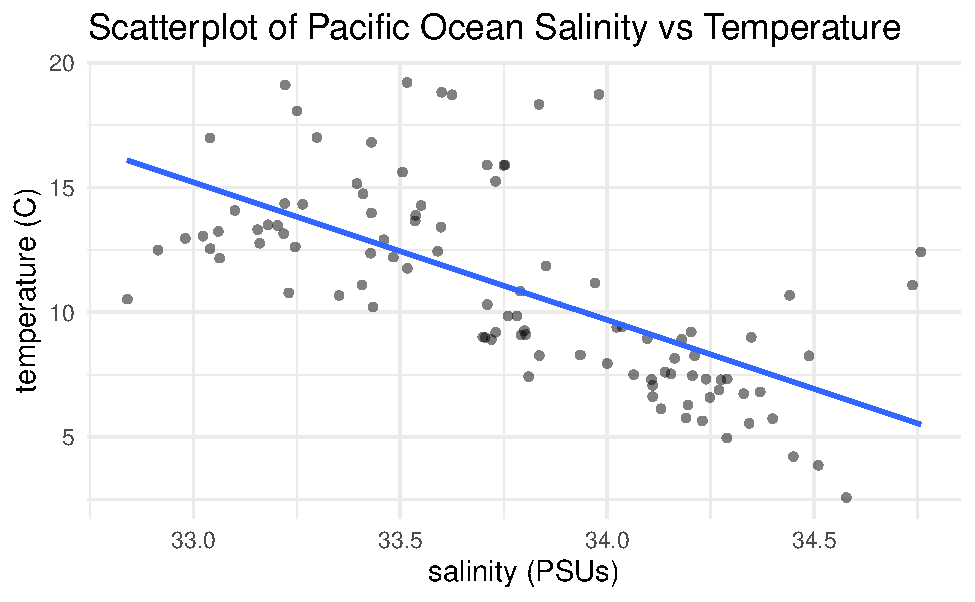
\includegraphics[width=0.7\linewidth]{13-VN13-regression_files/figure-latex/unnamed-chunk-10-1} \end{center}

Describe the four characteristics of the scatterplot:

\vspace{1in}

Linear model output:

\begin{Shaded}
\begin{Highlighting}[]
\NormalTok{lm.water }\OtherTok{\textless{}{-}} \FunctionTok{lm}\NormalTok{(T\_degC}\SpecialCharTok{\textasciitilde{}}\NormalTok{Salnty, }\AttributeTok{data=}\NormalTok{water) }\CommentTok{\# lm(response\textasciitilde{}explanatory)}
\FunctionTok{round}\NormalTok{(}\FunctionTok{summary}\NormalTok{(lm.water)}\SpecialCharTok{$}\NormalTok{coefficients, }\DecValTok{3}\NormalTok{)}
\end{Highlighting}
\end{Shaded}

\begin{verbatim}
#>             Estimate Std. Error t value Pr(>|t|)
#> (Intercept)  197.156     21.478    9.18        0
#> Salnty        -5.514      0.636   -8.67        0
\end{verbatim}

Correlation:

\begin{Shaded}
\begin{Highlighting}[]
\FunctionTok{cor}\NormalTok{(T\_degC}\SpecialCharTok{\textasciitilde{}}\NormalTok{Salnty, }\AttributeTok{data=}\NormalTok{water)}
\end{Highlighting}
\end{Shaded}

\begin{verbatim}
#> [1] -0.6588365
\end{verbatim}

Write the least squares equation of the line in context of the problem:

\vspace{0.5in}

Interpret the value of slope in the context of the problem:

\vspace{0.5in}

Report and describe the correlation value:

\vspace{0.5in}

Calculate and interpret the coefficient of determination:

\vspace{0.8in}

\subsubsection*{Simulation-based method}\label{simulation-based-method-3}
\addcontentsline{toc}{subsubsection}{Simulation-based method}

Conditions:

\begin{itemize}
\item
  Independence: the response for one observational unit will not influence another observational unit
\item
  Linear relationship:
\end{itemize}

\vspace{0.3in}

\begin{itemize}
\item
  Simulate many samples assuming \(H_0: \beta_1 = 0\) or \(H_0: \rho =0\)

  \begin{itemize}
  \item
    Write the response variable values on cards
  \item
    Hold the explanatory variable values constant
  \item
    Shuffle a new response variable to an explanatory variable
  \item
    Plot the shuffled data points to find the least squares line of regression
  \item
    Calculate and plot the simulated slope or correlation from each simulation
  \item
    Repeat 1000 times (simulations) to create the null distribution
  \item
    Find the proportion of simulations at least as extreme as \(b_1\) or \(r\)
  \end{itemize}
\end{itemize}

To test slope:

\begin{Shaded}
\begin{Highlighting}[]
\FunctionTok{set.seed}\NormalTok{(}\DecValTok{216}\NormalTok{)}
\FunctionTok{regression\_test}\NormalTok{(T\_degC }\SpecialCharTok{\textasciitilde{}}\NormalTok{ Salnty, }\CommentTok{\# response \textasciitilde{} explanatory}
               \AttributeTok{data =}\NormalTok{ water, }\CommentTok{\# Name of data set}
               \AttributeTok{direction =} \StringTok{"less"}\NormalTok{, }\CommentTok{\# Sign in alternative ("greater", "less", "two{-}sided")}
               \AttributeTok{summary\_measure =} \StringTok{"slope"}\NormalTok{, }\CommentTok{\# "slope" or "correlation"}
               \AttributeTok{as\_extreme\_as =} \SpecialCharTok{{-}}\FloatTok{5.514}\NormalTok{, }\CommentTok{\# Observed slope or correlation}
               \AttributeTok{number\_repetitions =} \DecValTok{10000}\NormalTok{) }\CommentTok{\# Number of simulated samples for null distribution}
\end{Highlighting}
\end{Shaded}

\begin{center}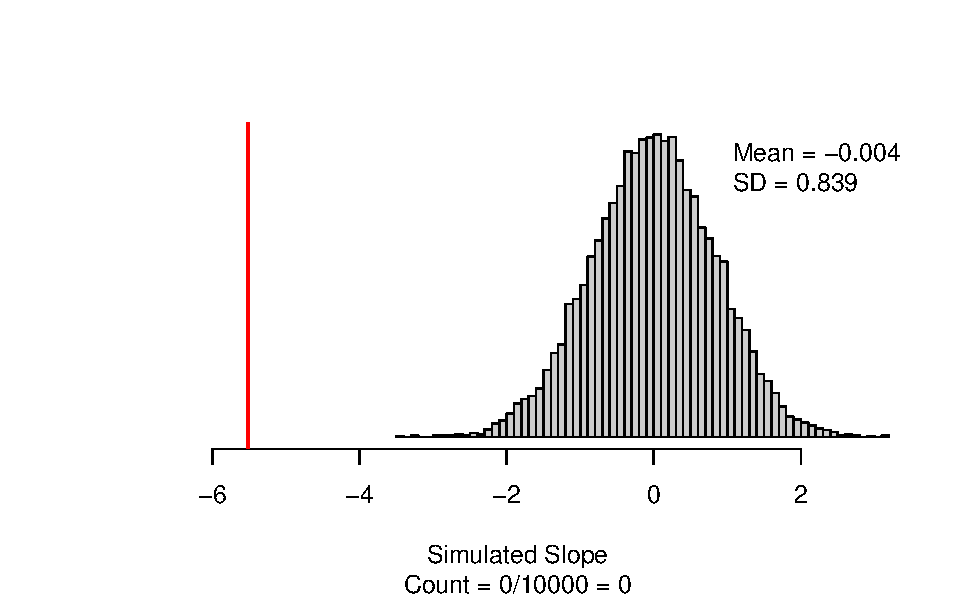
\includegraphics[width=0.7\linewidth]{13-VN13-regression_files/figure-latex/unnamed-chunk-13-1} \end{center}

\newpage

To test correlation:

\begin{Shaded}
\begin{Highlighting}[]
\FunctionTok{set.seed}\NormalTok{(}\DecValTok{216}\NormalTok{)}
\FunctionTok{regression\_test}\NormalTok{(T\_degC}\SpecialCharTok{\textasciitilde{}}\NormalTok{Salnty, }\CommentTok{\# response \textasciitilde{} explanatory}
               \AttributeTok{data =}\NormalTok{ water, }\CommentTok{\# Name of data set}
               \AttributeTok{direction =} \StringTok{"less"}\NormalTok{, }\CommentTok{\# Sign in alternative ("greater", "less", "two{-}sided")}
               \AttributeTok{summary\_measure =} \StringTok{"correlation"}\NormalTok{, }\CommentTok{\# "slope" or "correlation"}
               \AttributeTok{as\_extreme\_as =} \SpecialCharTok{{-}}\FloatTok{0.659}\NormalTok{, }\CommentTok{\# Observed slope or correlation}
               \AttributeTok{number\_repetitions =} \DecValTok{10000}\NormalTok{) }\CommentTok{\# Number of simulated samples for null distribution}
\end{Highlighting}
\end{Shaded}

\begin{center}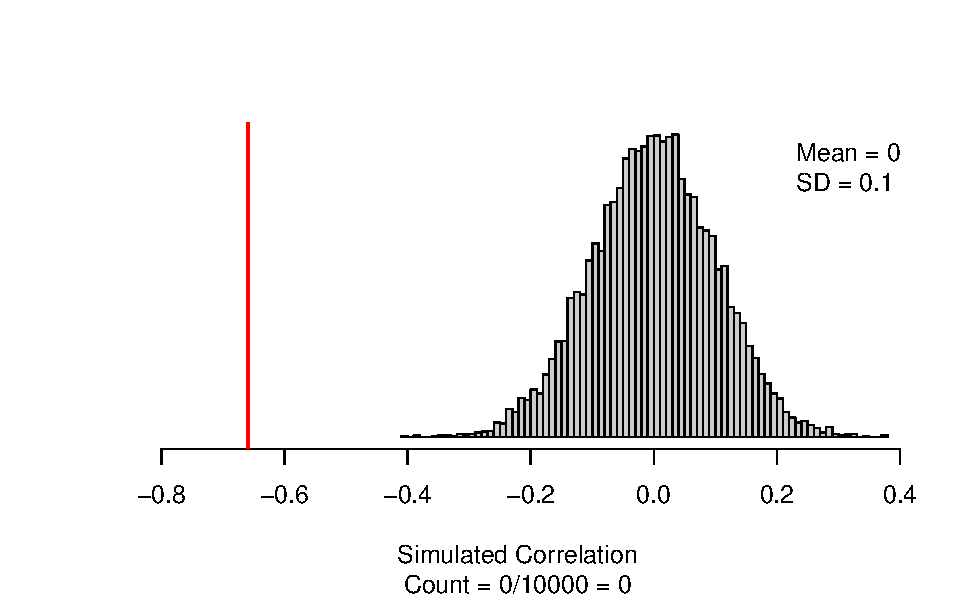
\includegraphics[width=0.7\linewidth]{13-VN13-regression_files/figure-latex/unnamed-chunk-14-1} \end{center}

Explain why the null distribution is centered at the value of zero:

\vspace{0.5in}

Interpretation of the p-value:

\begin{itemize}
\item
  Statement about probability or proportion of samples
\item
  Statistic (summary measure and value)
\item
  Direction of the alternative
\item
  Null hypothesis (in context)
\end{itemize}

\vspace{0.8in}

Conclusion:

\begin{itemize}
\item
  Amount of evidence
\item
  Parameter of interest
\item
  Direction of the alternative hypothesis
\end{itemize}

\vspace{0.6in}

\subsection*{Confidence interval - Video 21.3}\label{confidence-interval---video-21.3}
\addcontentsline{toc}{subsection}{Confidence interval - Video 21.3}

To estimate the true slope (or true correlation) we will create a confidence interval.

\subsubsection*{Simulation-based method}\label{simulation-based-method-4}
\addcontentsline{toc}{subsubsection}{Simulation-based method}

\begin{itemize}
\item
  Write the explanatory and response value pairs on cards
\item
  Sample pairs with replacement \(n\) times
\item
  Plot the resampled data points to find the least squares line of regression
\item
  Calculate and plot the simulated slope (or correlation) from each simulation
\item
  Repeat 1000 times (simulations) to create the bootstrap distribution
\item
  Find the cut-offs for the middle X\% (confidence level) in a bootstrap distribution.
\end{itemize}

Returning to the ocean example, we will estimate the true slope between salinity and temperature of the Pacific Ocean.

\begin{Shaded}
\begin{Highlighting}[]
\FunctionTok{set.seed}\NormalTok{(}\DecValTok{216}\NormalTok{)}
\FunctionTok{regression\_bootstrap\_CI}\NormalTok{(T\_degC}\SpecialCharTok{\textasciitilde{}}\NormalTok{Salnty, }\CommentTok{\# response \textasciitilde{} explanatory}
   \AttributeTok{data =}\NormalTok{ water, }\CommentTok{\# Name of data set}
   \AttributeTok{confidence\_level =} \FloatTok{0.95}\NormalTok{, }\CommentTok{\# Confidence level as decimal}
   \AttributeTok{summary\_measure =} \StringTok{"slope"}\NormalTok{, }\CommentTok{\# Slope or correlation}
   \AttributeTok{number\_repetitions =} \DecValTok{10000}\NormalTok{) }\CommentTok{\# Number of simulated samples for bootstrap distribution}
\end{Highlighting}
\end{Shaded}

\begin{center}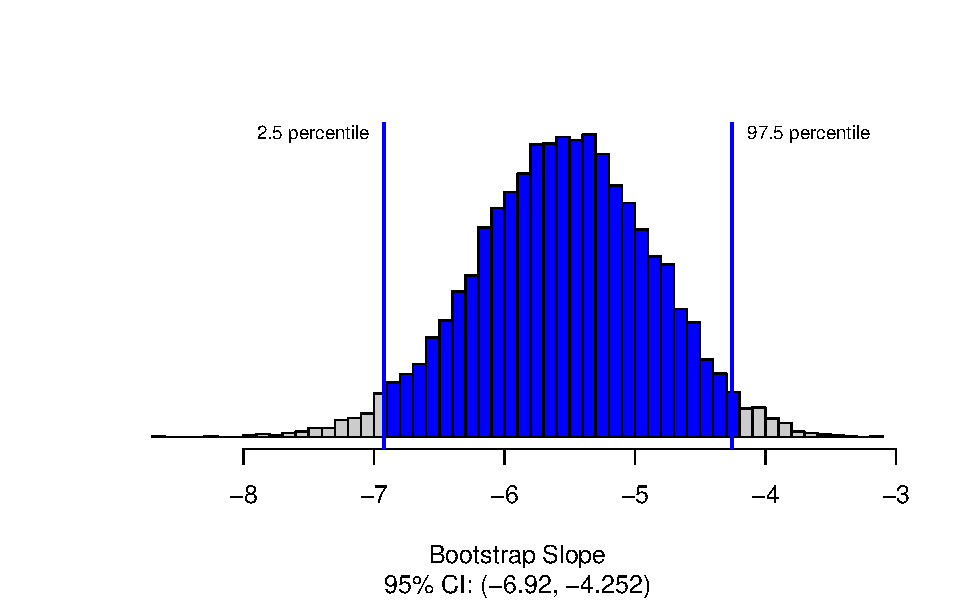
\includegraphics[width=0.7\linewidth]{13-VN13-regression_files/figure-latex/unnamed-chunk-15-1} \end{center}

Confidence interval interpretation:

\begin{itemize}
\item
  How confident you are (e.g., 90\%, 95\%, 98\%, 99\%)
\item
  Parameter of interest
\item
  Calculated interval
\item
  Order of subtraction when comparing two groups
\end{itemize}

\vspace{0.8in}

Now we will estimate the true correlation between salinity and temperature of the Pacific Ocean.

\begin{Shaded}
\begin{Highlighting}[]
\FunctionTok{set.seed}\NormalTok{(}\DecValTok{216}\NormalTok{)}
\FunctionTok{regression\_bootstrap\_CI}\NormalTok{(T\_degC}\SpecialCharTok{\textasciitilde{}}\NormalTok{Salnty, }\CommentTok{\# response \textasciitilde{} explanatory}
   \AttributeTok{data =}\NormalTok{ water, }\CommentTok{\# Name of data set}
   \AttributeTok{confidence\_level =} \FloatTok{0.95}\NormalTok{, }\CommentTok{\# Confidence level as decimal}
   \AttributeTok{summary\_measure =} \StringTok{"correlation"}\NormalTok{, }\CommentTok{\# Slope or correlation}
   \AttributeTok{number\_repetitions =} \DecValTok{10000}\NormalTok{) }\CommentTok{\# Number of simulated samples for bootstrap distribution}
\end{Highlighting}
\end{Shaded}

\begin{center}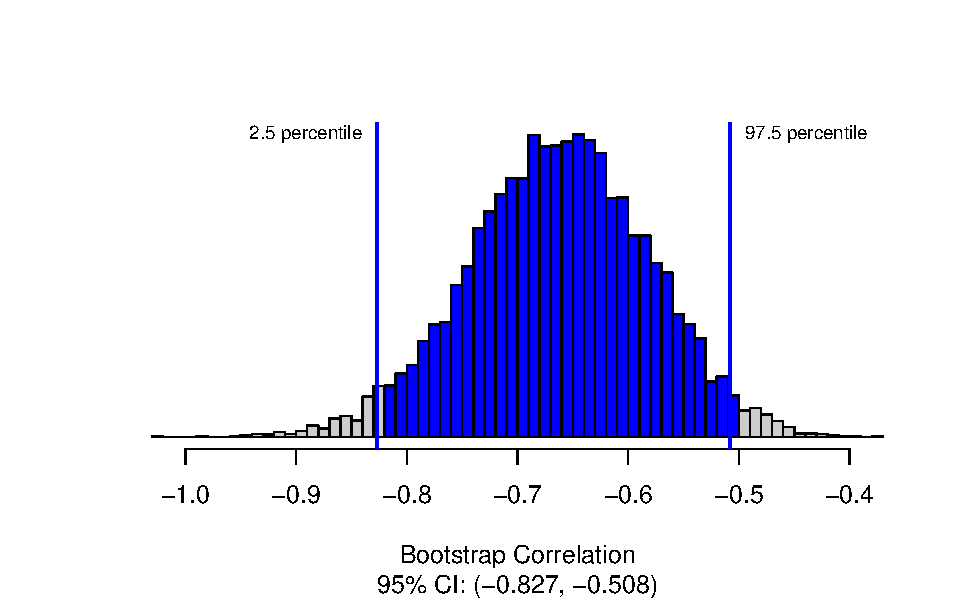
\includegraphics[width=0.7\linewidth]{13-VN13-regression_files/figure-latex/unnamed-chunk-16-1} \end{center}

Confidence interval interpretation:

\begin{itemize}
\item
  How confident you are (e.g., 90\%, 95\%, 98\%, 99\%)
\item
  Parameter of interest
\item
  Calculated interval
\item
  Order of subtraction when comparing two groups
\end{itemize}

\vspace{0.8in}

\subsubsection*{Theory-based method - Video 21.4to21.5TheoryTests}\label{theory-based-method---video-21.4to21.5theorytests}
\addcontentsline{toc}{subsubsection}{Theory-based method - Video 21.4to21.5TheoryTests}

Conditions:

\setstretch{1.5}

\begin{itemize}
\item
  Linearity (for both simulation-based and theory-based methods): the data should follow a linear trend.

  \begin{itemize}
  \tightlist
  \item
    Check this assumption by examining the \_\_\_\_\_\_\_\_\_\_\_\_\_\_\_\_\_\_\_\_\_\_\_\_\_\_\_\_ of the two variables, and \_\_\_\_\_\_\_\_\_\_\_\_\_\_\_\_\_\_\_\_\_\_\_\_\_\_\_\_\_\_\_\_\_\_\_\_\_\_\_\_\_\_\_\_. The pattern in the residual plot should display a horizontal line.
  \end{itemize}
\end{itemize}

\newpage

\begin{itemize}
\item
  Independence (for both simulation-based and theory-based methods)

  \begin{itemize}
  \tightlist
  \item
    One\_\_\_\_\_\_\_\_\_\_\_\_\_\_\_\_\_\_\_\_\_\_\_\_\_\_\_\_\_\_for an observational unit has no impact on \_\_\_\_\_\_\_\_\_\_\_\_\_\_\_\_\_\_\_\_\_\_\_\_\_\_\_\_\_\_\_\_.
  \end{itemize}
\item
  Constant variability (for theory-based methods only): the variability of points around the least squares line remains roughly constant

  \begin{itemize}
  \tightlist
  \item
    Check this assumption by examining the \_\_\_\_\_\_\_\_\_\_\_\_\_\_\_\_\_\_\_\_\_\_\_\_\_\_\_\_\_\_\_\_. The variability in the residuals around zero should be approximately the same for all fitted values.
  \end{itemize}
\item
  Nearly normal residuals (for theory-based methods only): residuals must be nearly normal

  \begin{itemize}
  \tightlist
  \item
    Check this assumption by examining a \_\_\_\_\_\_\_\_\_\_\_\_\_\_\_\_\_\_\_\_\_\_\_\_\_\_\_\_\_\_\_\_\_, which should appear approximately normal
  \end{itemize}
\end{itemize}

\setstretch{1}

Example:

It is a generally accepted fact that the more carats a diamond has, the more expensive that diamond will be. The question is, how much more expensive? Data on thousands of diamonds were collected for this data set. We will only look at one type of cut (``Ideal'') and diamonds less than 1 carat. Does the association between carat size and price have a linear relationship for these types of diamonds? What can we state about the association between carat size and price?

Scatterplot:

\begin{Shaded}
\begin{Highlighting}[]
\NormalTok{Diamonds }\SpecialCharTok{\%\textgreater{}\%} \CommentTok{\# Pipe data set into...}
    \FunctionTok{ggplot}\NormalTok{(}\FunctionTok{aes}\NormalTok{(}\AttributeTok{x =}\NormalTok{ carat, }\AttributeTok{y =}\NormalTok{ price))}\SpecialCharTok{+}  \CommentTok{\# Specify variables}
    \FunctionTok{geom\_point}\NormalTok{(}\AttributeTok{alpha=}\FloatTok{0.5}\NormalTok{) }\SpecialCharTok{+}  \CommentTok{\# Add scatterplot of points}
    \FunctionTok{labs}\NormalTok{(}\AttributeTok{x =} \StringTok{"carat"}\NormalTok{,  }\CommentTok{\# Label x{-}axis}
       \AttributeTok{y =} \StringTok{"price ($)"}\NormalTok{,  }\CommentTok{\# Label y{-}axis}
       \AttributeTok{title =} \StringTok{"Scatterplot of Diamonds Carats vs Price"}\NormalTok{) }\SpecialCharTok{+}
               \CommentTok{\# Be sure to title your plots}
    \FunctionTok{geom\_smooth}\NormalTok{(}\AttributeTok{method =} \StringTok{"lm"}\NormalTok{, }\AttributeTok{se =} \ConstantTok{FALSE}\NormalTok{)  }\CommentTok{\# Add regression line}
\end{Highlighting}
\end{Shaded}

\begin{center}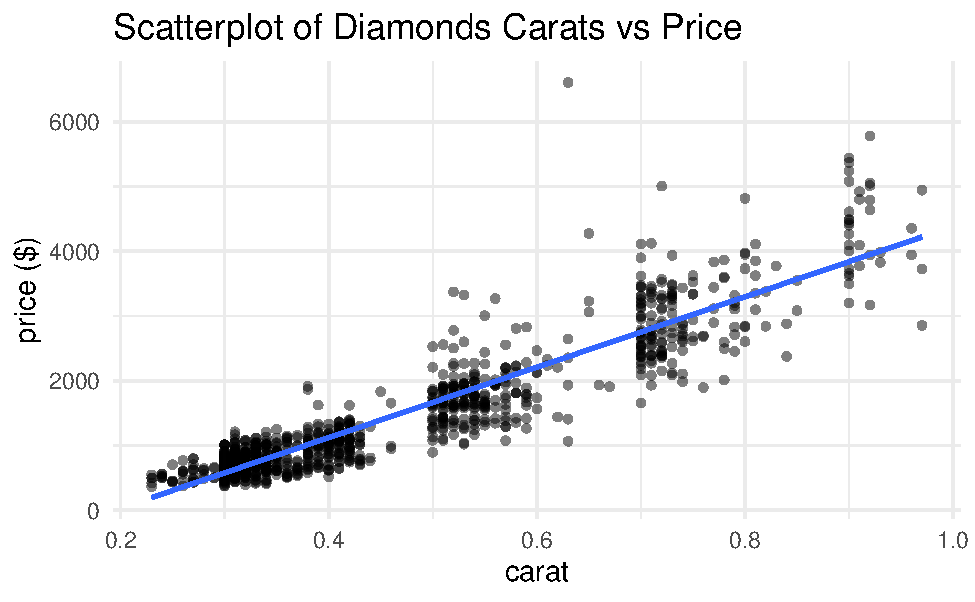
\includegraphics[width=0.7\linewidth]{13-VN13-regression_files/figure-latex/unnamed-chunk-18-1} \end{center}

\newpage

Diagnostic plots:

\begin{center}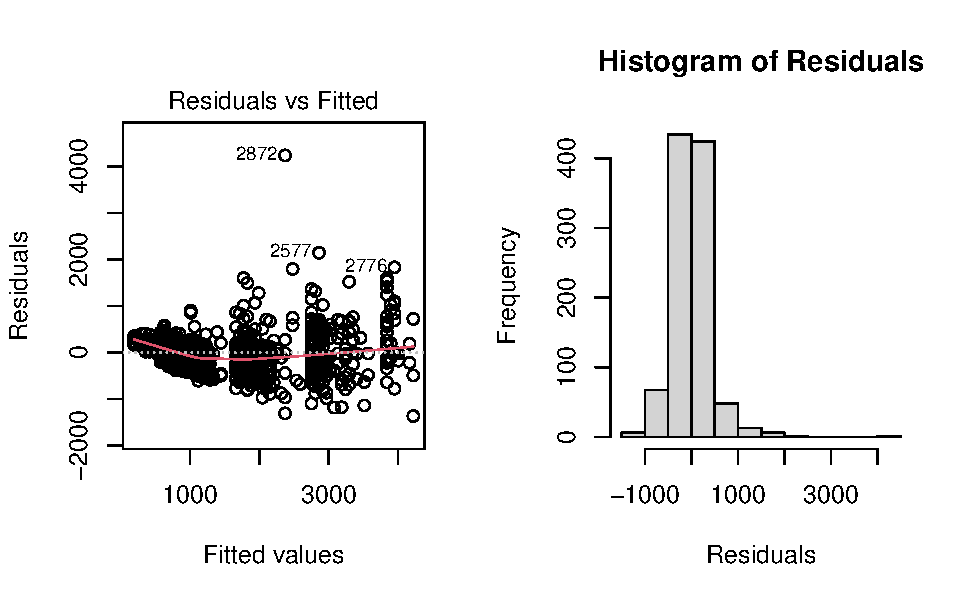
\includegraphics[width=0.7\linewidth]{13-VN13-regression_files/figure-latex/unnamed-chunk-19-1} \end{center}

Check the conditions for the ocean data:

Scatterplot:

\begin{Shaded}
\begin{Highlighting}[]
\NormalTok{water }\SpecialCharTok{\%\textgreater{}\%} \CommentTok{\# Pipe data set into...}
\FunctionTok{ggplot}\NormalTok{(}\FunctionTok{aes}\NormalTok{(}\AttributeTok{x =}\NormalTok{ Salnty, }\AttributeTok{y =}\NormalTok{ T\_degC))}\SpecialCharTok{+}  \CommentTok{\# Specify variables}
  \FunctionTok{geom\_point}\NormalTok{(}\AttributeTok{alpha=}\FloatTok{0.5}\NormalTok{) }\SpecialCharTok{+}  \CommentTok{\# Add scatterplot of points}
  \FunctionTok{labs}\NormalTok{(}\AttributeTok{x =} \StringTok{"salinity (PSUs)"}\NormalTok{,  }\CommentTok{\# Label x{-}axis}
       \AttributeTok{y =} \StringTok{"temperature (C)"}\NormalTok{,  }\CommentTok{\# Label y{-}axis}
       \AttributeTok{title =} \StringTok{"Scatterplot of Pacific Ocean Salinity vs Temperature"}\NormalTok{) }\SpecialCharTok{+} 
               \CommentTok{\# Be sure to title your plots}
  \FunctionTok{geom\_smooth}\NormalTok{(}\AttributeTok{method =} \StringTok{"lm"}\NormalTok{, }\AttributeTok{se =} \ConstantTok{FALSE}\NormalTok{)  }\CommentTok{\# Add regression line}
\end{Highlighting}
\end{Shaded}

\begin{center}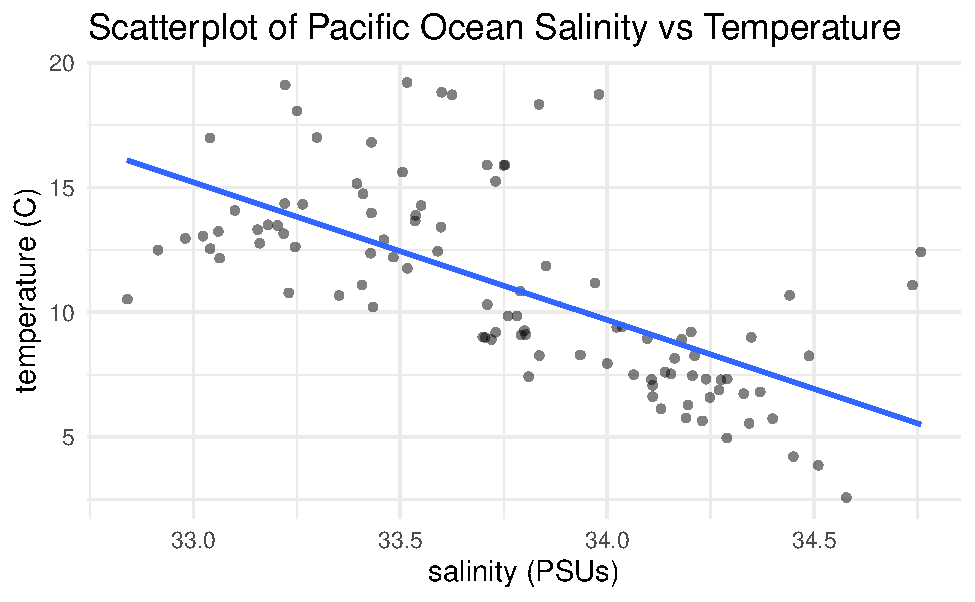
\includegraphics[width=0.7\linewidth]{13-VN13-regression_files/figure-latex/unnamed-chunk-20-1} \end{center}

\newpage

Diagnostic plots:

\begin{center}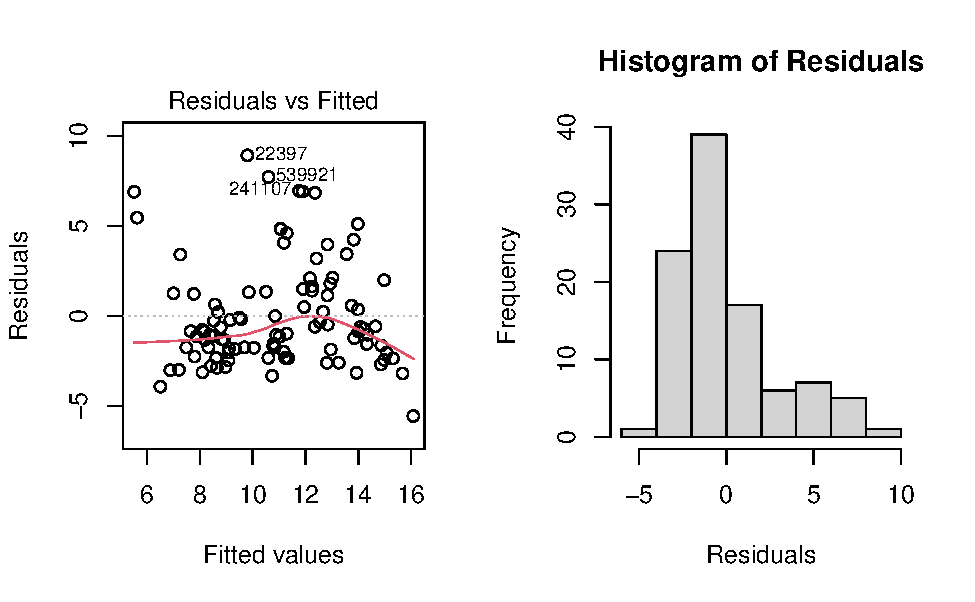
\includegraphics[width=0.7\linewidth]{13-VN13-regression_files/figure-latex/unnamed-chunk-21-1} \end{center}

Like with paired data the \(t\)-distribution can be used to model slope and correlation.

\setstretch{1.5}

\begin{itemize}
\tightlist
\item
  For two quantitative variables we use the \_\_\_\_\_\_-distribution
  with \_\_\_\_\_\_\_\_\_\_\_\_\_\_\_\_\_\_\_\_\_ degrees of freedom to approximate the sampling distribution.
\end{itemize}

\setstretch{1}

Theory-based test:

\begin{itemize}
\item
  Calculate the standardized statistic
\item
  Find the area under the \(t\)-distribution with \(n - 2\) df at least as extreme as the standardized statistic
\end{itemize}

Equation for the standardized slope:

\vspace{0.8in}

Calculate the standardized slope for the ocean data

\begin{Shaded}
\begin{Highlighting}[]
\NormalTok{lm.water }\OtherTok{\textless{}{-}} \FunctionTok{lm}\NormalTok{(T\_degC}\SpecialCharTok{\textasciitilde{}}\NormalTok{Salnty, }\AttributeTok{data=}\NormalTok{water) }\CommentTok{\# lm(response\textasciitilde{}explanatory)}
\FunctionTok{round}\NormalTok{(}\FunctionTok{summary}\NormalTok{(lm.water)}\SpecialCharTok{$}\NormalTok{coefficients,}\DecValTok{3}\NormalTok{)}
\end{Highlighting}
\end{Shaded}

\begin{verbatim}
#>             Estimate Std. Error t value Pr(>|t|)
#> (Intercept)  197.156     21.478    9.18        0
#> Salnty        -5.514      0.636   -8.67        0
\end{verbatim}

\vspace{1in}

\begin{center}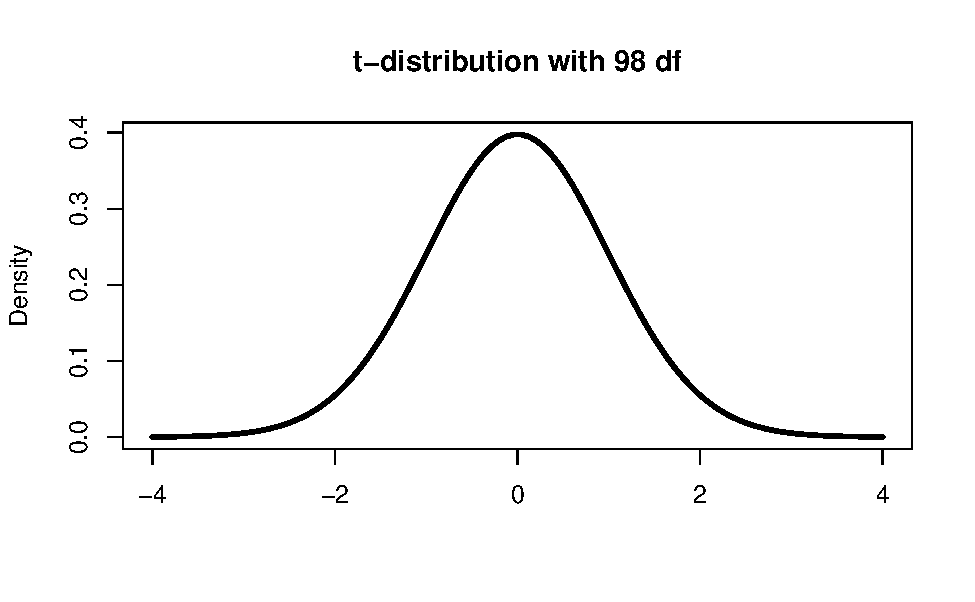
\includegraphics[width=0.7\linewidth]{13-VN13-regression_files/figure-latex/pvalueoce-1} \end{center}

Interpret the standardized statistic:

\vspace{0.8in}

To find the theory-based p-value:

\begin{Shaded}
\begin{Highlighting}[]
\NormalTok{lm.water }\OtherTok{\textless{}{-}} \FunctionTok{lm}\NormalTok{(T\_degC}\SpecialCharTok{\textasciitilde{}}\NormalTok{Salnty, }\AttributeTok{data=}\NormalTok{water) }\CommentTok{\# lm(response\textasciitilde{}explanatory)}
\FunctionTok{round}\NormalTok{(}\FunctionTok{summary}\NormalTok{(lm.water)}\SpecialCharTok{$}\NormalTok{coefficients,}\DecValTok{3}\NormalTok{)}
\end{Highlighting}
\end{Shaded}

\begin{verbatim}
#>             Estimate Std. Error t value Pr(>|t|)
#> (Intercept)  197.156     21.478    9.18        0
#> Salnty        -5.514      0.636   -8.67        0
\end{verbatim}

or

\begin{Shaded}
\begin{Highlighting}[]
\FunctionTok{pt}\NormalTok{(}\SpecialCharTok{{-}}\FloatTok{8.670}\NormalTok{, }\AttributeTok{df =} \DecValTok{98}\NormalTok{, }\AttributeTok{lower.tail=}\ConstantTok{TRUE}\NormalTok{)}
\CommentTok{\#\textgreater{} [1] 4.623445e{-}14}
\end{Highlighting}
\end{Shaded}

\newpage

\subsubsection*{Theory-based method}\label{theory-based-method}
\addcontentsline{toc}{subsubsection}{Theory-based method}

\begin{itemize}
\tightlist
\item
  Calculate the interval centered at the sample statistic
\end{itemize}

\rgi \(\text{statistic} \pm \text{margin of error}\)

\vspace{0.6in}

\begin{Shaded}
\begin{Highlighting}[]
\NormalTok{lm.water }\OtherTok{\textless{}{-}} \FunctionTok{lm}\NormalTok{(T\_degC}\SpecialCharTok{\textasciitilde{}}\NormalTok{Salnty, }\AttributeTok{data=}\NormalTok{water) }\CommentTok{\# lm(response\textasciitilde{}explanatory)}
\FunctionTok{round}\NormalTok{(}\FunctionTok{summary}\NormalTok{(lm.water)}\SpecialCharTok{$}\NormalTok{coefficients, }\DecValTok{3}\NormalTok{)}
\end{Highlighting}
\end{Shaded}

\begin{verbatim}
#>             Estimate Std. Error t value Pr(>|t|)
#> (Intercept)  197.156     21.478    9.18        0
#> Salnty        -5.514      0.636   -8.67        0
\end{verbatim}

Using the ocean data, calculate a 95\% confidence interval for the true slope.

\begin{itemize}
\tightlist
\item
  Need the \(t^*\) multiplier for a 95\% confidence interval from a t-distribution with \_\_\_\_\_\_\_\_\_ df.
\end{itemize}

\begin{Shaded}
\begin{Highlighting}[]
\FunctionTok{qt}\NormalTok{(}\FloatTok{0.975}\NormalTok{, }\AttributeTok{df=}\DecValTok{98}\NormalTok{, }\AttributeTok{lower.tail =} \ConstantTok{TRUE}\NormalTok{)}
\end{Highlighting}
\end{Shaded}

\begin{verbatim}
#> [1] 1.984467
\end{verbatim}

\vspace{1in}

\subsection{Concept Check}\label{concept-check-3}

Be prepared for group discussion in the next class. One member from the table should write the answers to the following on the whiteboard.

\begin{enumerate}
\def\labelenumi{\arabic{enumi}.}
\tightlist
\item
  Explain why theory-based methods should not be used to analyze the salinity study?
\end{enumerate}

\vspace{0.6in}

\begin{enumerate}
\def\labelenumi{\arabic{enumi}.}
\setcounter{enumi}{1}
\tightlist
\item
  What is the proper notation for the population slope? Population correlation?
\end{enumerate}

\vspace{0.4in}

\newpage

\section{Activity 26: Moneyball --- Linear Regression}\label{activity-26-moneyball-linear-regression}

\setstretch{1}

\subsection{Learning outcomes}\label{learning-outcomes-7}

\begin{itemize}
\item
  Identify and create appropriate summary statistics and plots
  given a data set with two quantitative variables.
\item
  Use scatterplots to assess the relationship between two quantitative variables.
\item
  Find the estimated line of regression using summary statistics and \texttt{R} linear model (\texttt{lm()}) output.
\item
  Interpret the slope coefficient in context of the problem.
\end{itemize}

\subsection{Terminology review}\label{terminology-review-5}

In today's activity, we will review summary measures and plots for two quantitative variables. Some terms covered in this activity are:

\begin{itemize}
\item
  Scatterplot
\item
  Least-squares line of regression
\item
  Slope and \(y\)-intercept
\item
  Residuals
\end{itemize}

To review these concepts, see Chapter 6 \& 7 in the textbook.

\subsection{Moneyball}\label{moneyball}

The goal of a Major League baseball team is to make the playoffs. In 2002, the manager of the Oakland A's, Billy Bean, with the help of Paul DePodesta began to use statistics to determine which players to choose for their season. Based on past data, DePodesta determined that to make it to the playoffs, the A's would need to win at least 95 games in the regular season. In order to win more games, they would need to score more runs than they allowed. The Oakland A's won 20 consecutive games and a total of 103 games for the season. The success of this use of sports analytics was portrayed by the 2011 movie, Moneyball. In this study, we will see if there is evidence of a positive linear relationship between the difference in the number of runs scored minus the number of runs allowed (\texttt{RD}) and the number of wins for Major League baseball teams in the years before 2002. Some of the variables collected in the data set baseball consist of the following:

\begin{longtable}[]{@{}ll@{}}
\toprule\noalign{}
\textbf{Variable} & \textbf{Description} \\
\midrule\noalign{}
\endhead
\bottomrule\noalign{}
\endlastfoot
\texttt{RA} & Runs allowed \\
\texttt{RS} & Runs scored \\
\texttt{OBP} & On-base percentage \\
\texttt{SLG} & Slugging percentage \\
\texttt{BA} & Batting average \\
\texttt{OOBP} & Opponent's on-base percentage \\
\texttt{OSLG} & Opponent's slugging percentage \\
\texttt{W} & Number of wins in the season \\
\texttt{RD} & Difference of runs scored minus runs allowed \\
\end{longtable}

\begin{Shaded}
\begin{Highlighting}[]
\NormalTok{moneyball }\OtherTok{\textless{}{-}} \FunctionTok{read.csv}\NormalTok{(}\StringTok{"data/baseball.csv"}\NormalTok{) }\CommentTok{\# Reads in data set }
\NormalTok{moneyball}\SpecialCharTok{$}\NormalTok{RD }\OtherTok{\textless{}{-}}\NormalTok{ moneyball}\SpecialCharTok{$}\NormalTok{RS }\SpecialCharTok{{-}}\NormalTok{ moneyball}\SpecialCharTok{$}\NormalTok{RA}
\NormalTok{moneyball }\OtherTok{\textless{}{-}} 
\NormalTok{    moneyball }\SpecialCharTok{\%\textgreater{}\%} \CommentTok{\# Pipe data set into}
    \FunctionTok{subset}\NormalTok{(Year }\SpecialCharTok{\textless{}} \DecValTok{2002}\NormalTok{) }\CommentTok{\# Select only years before 2002}
\end{Highlighting}
\end{Shaded}

\subsubsection*{Vocabulary review}\label{vocabulary-review}
\addcontentsline{toc}{subsubsection}{Vocabulary review}

\begin{itemize}
\item
  Use the provided R script file to create a scatterplot to examine the relationship between the difference in number of runs scored minus number of runs allowed and the number of wins by filling in the variable names (RD and W) for explanatory and response in line 14. Note, we are using the difference in runs scores minus runs allowed to predict the number of season wins.
\item
  Highlight and run lines 1--20.
\end{itemize}

\begin{Shaded}
\begin{Highlighting}[]
\NormalTok{moneyball }\SpecialCharTok{\%\textgreater{}\%} \CommentTok{\# Data set pipes into...}
    \FunctionTok{ggplot}\NormalTok{(}\FunctionTok{aes}\NormalTok{(}\AttributeTok{x =}\NormalTok{ explanatory, }\AttributeTok{y =}\NormalTok{ response))}\SpecialCharTok{+} \CommentTok{\# Specify variables}
    \FunctionTok{geom\_point}\NormalTok{() }\SpecialCharTok{+} \CommentTok{\# Add scatterplot of points}
    \FunctionTok{labs}\NormalTok{(}\AttributeTok{x =} \StringTok{"Difference in number of runs"}\NormalTok{, }\CommentTok{\# Label x{-}axis}
         \AttributeTok{y =} \StringTok{"Number of Season wins"}\NormalTok{, }\CommentTok{\# Label y{-}axis}
         \AttributeTok{title =} \StringTok{"Scatterplot of Run Difference vs. Number of Season Wins for MLB Teams"}\NormalTok{) }\SpecialCharTok{+}
\CommentTok{\# Be sure to tile your plots}
\FunctionTok{geom\_smooth}\NormalTok{(}\AttributeTok{method =} \StringTok{"lm"}\NormalTok{, }\AttributeTok{se =} \ConstantTok{FALSE}\NormalTok{) }\CommentTok{\# Add regression line}
\end{Highlighting}
\end{Shaded}

\begin{enumerate}
\def\labelenumi{\arabic{enumi}.}
\tightlist
\item
  Assess the four features of the scatterplot that describe this relationship.
\end{enumerate}

\begin{itemize}
\tightlist
\item
  Form (linear, non-linear)
\end{itemize}

\vspace{.075in}

\begin{itemize}
\tightlist
\item
  Direction (positive, negative)
\end{itemize}

\vspace{.075in}

\begin{itemize}
\tightlist
\item
  Strength
\end{itemize}

\vspace{.075in}

\begin{itemize}
\tightlist
\item
  Unusual observations or outliers
\end{itemize}

\vspace{.075in}

\begin{enumerate}
\def\labelenumi{\arabic{enumi}.}
\setcounter{enumi}{1}
\tightlist
\item
  Based on the plot, does there appear to be an association between run difference and number of season wins? Explain your answer.
\end{enumerate}

\vspace{1in}

\subsubsection*{Slope}\label{slope-1}
\addcontentsline{toc}{subsubsection}{Slope}

The linear model function in R (\texttt{lm()}) gives us the summary for the least squares regression line. The estimate for \texttt{(Intercept)} is the \(y\)-intercept for the line of least squares, and the estimate for \texttt{budget\_mil} (the \(x\)-variable name) is the value of \(b_1\), the slope.

\begin{itemize}
\tightlist
\item
  Run lines 24--25 in the R script file to reproduce the linear model output found in the coursepack.
\end{itemize}

\begin{Shaded}
\begin{Highlighting}[]
\CommentTok{\# Fit linear model: y \textasciitilde{} x}
\NormalTok{moneyballLM }\OtherTok{\textless{}{-}} \FunctionTok{lm}\NormalTok{(W}\SpecialCharTok{\textasciitilde{}}\NormalTok{RD, }\AttributeTok{data=}\NormalTok{moneyball)}
\FunctionTok{round}\NormalTok{(}\FunctionTok{summary}\NormalTok{(moneyballLM)}\SpecialCharTok{$}\NormalTok{coefficients, }\DecValTok{3}\NormalTok{) }\CommentTok{\# Display coefficient summary}
\end{Highlighting}
\end{Shaded}

\begin{verbatim}
#>             Estimate Std. Error t value Pr(>|t|)
#> (Intercept)   80.881      0.131 616.675        0
#> RD             0.106      0.001  81.554        0
\end{verbatim}

\begin{enumerate}
\def\labelenumi{\arabic{enumi}.}
\setcounter{enumi}{2}
\item
  Write out the least squares regression line using the summary statistics provided above in context of the problem.
  \vspace{0.8in}
\item
  Interpret the value of slope in context of the problem.
\end{enumerate}

\vspace{.8in}

\begin{enumerate}
\def\labelenumi{\arabic{enumi}.}
\setcounter{enumi}{4}
\tightlist
\item
  Using the least squares line from question 3, predict the number of season wins for a MLB team that has a run difference of -66 runs.
\end{enumerate}

\vspace{.6in}

\begin{enumerate}
\def\labelenumi{\arabic{enumi}.}
\setcounter{enumi}{5}
\tightlist
\item
  Predict the number of season wins for a MLB team that has a run difference of 400 runs.
\end{enumerate}

\vspace{0.8in}

\begin{enumerate}
\def\labelenumi{\arabic{enumi}.}
\setcounter{enumi}{6}
\tightlist
\item
  The prediction in question 6 is an example of what?
\end{enumerate}

\vspace{0.3in}

\subsubsection*{Residuals}\label{residuals}
\addcontentsline{toc}{subsubsection}{Residuals}

The model we are using assumes the relationship between the two variables follows a straight line. The residuals are the errors, or the variability in the response that hasn't been modeled by the regression line.

\begin{center}

$\implies$ Residual = actual y value $-$ predicted y value

$e=y-\hat{y}$
\end{center}

\begin{enumerate}
\def\labelenumi{\arabic{enumi}.}
\setcounter{enumi}{7}
\tightlist
\item
  The MLB team \emph{Florida Marlins} had a run difference of -66 runs and 79 wins for the season. Find the residual for this MLB team.
\end{enumerate}

\vspace{.8in}

\begin{enumerate}
\def\labelenumi{\arabic{enumi}.}
\setcounter{enumi}{8}
\tightlist
\item
  Did the line of regression overestimate or underestimate the number of wins for the season for this team?
\end{enumerate}

\vspace{.2in}

\newpage

\subsubsection*{Correlation}\label{correlation-1}
\addcontentsline{toc}{subsubsection}{Correlation}

The following output shows a correlation matrix between several pairs of quantitative variables.

\begin{itemize}
\tightlist
\item
  Highlight and run lines 29--33 to produce the same table as below.
\end{itemize}

\begin{Shaded}
\begin{Highlighting}[]
\NormalTok{moneyball }\SpecialCharTok{\%\textgreater{}\%}  \CommentTok{\# Data set pipes into}
  \FunctionTok{select}\NormalTok{(}\FunctionTok{c}\NormalTok{(}\StringTok{"RD"}\NormalTok{, }\StringTok{"BA"}\NormalTok{, }
           \StringTok{"SLG"}\NormalTok{, }\StringTok{"W"}\NormalTok{)) }\SpecialCharTok{\%\textgreater{}\%}
  \FunctionTok{cor}\NormalTok{(}\AttributeTok{use=}\StringTok{"pairwise.complete.obs"}\NormalTok{) }\SpecialCharTok{\%\textgreater{}\%}
  \FunctionTok{round}\NormalTok{(}\DecValTok{3}\NormalTok{)}
\end{Highlighting}
\end{Shaded}

\begin{verbatim}
#>        RD    BA   SLG     W
#> RD  1.000 0.442 0.428 0.939
#> BA  0.442 1.000 0.814 0.416
#> SLG 0.428 0.814 1.000 0.406
#> W   0.939 0.416 0.406 1.000
\end{verbatim}

\begin{enumerate}
\def\labelenumi{\arabic{enumi}.}
\setcounter{enumi}{9}
\tightlist
\item
  Report the value of correlation between the run difference and the number of season wins.
\end{enumerate}

\vspace{0.3in}

\begin{enumerate}
\def\labelenumi{\arabic{enumi}.}
\setcounter{enumi}{10}
\tightlist
\item
  Calculate the coefficient of determination between the run difference and the number of season wins.
\end{enumerate}

\vspace{0.5in}

\begin{enumerate}
\def\labelenumi{\arabic{enumi}.}
\setcounter{enumi}{11}
\tightlist
\item
  Interpret the value of coefficient of determination in context of the study.
\end{enumerate}

\vspace{0.7in}

\subsection{Take-home messages}\label{take-home-messages-5}

\begin{enumerate}
\def\labelenumi{\arabic{enumi}.}
\item
  Two quantitative variables are graphically displayed in a scatterplot. The explanatory variable is on the \(x\)-axis and the response variable is on the \(y\)-axis. When describing the relationship between two quantitative variables we look at the form (linear or non-linear), direction (positive or negative), strength, and for the presence of outliers.
\item
  There are three summary statistics used to summarize the relationship between two quantitative variables: correlation (\(r\)), slope of the regression line (\(b_1\)), and the coefficient of determination (\(r^2\)).
\end{enumerate}

\subsection{Additional notes}\label{additional-notes-5}

Use this space to summarize your thoughts and take additional notes on today's activity and material covered.

\newpage

\section{Activity 27: IPEDS (continued)}\label{activity-27-ipeds-continued}

\setstretch{1}

\subsection{Learning outcomes}\label{learning-outcomes-8}

\begin{itemize}
\item
  Identify and create appropriate summary statistics and plots
  given a data set with two quantitative variables.
\item
  Find the estimated line of regression using summary statistics and \texttt{R} linear model (\texttt{lm()}) output.
\item
  Interpret the slope coefficient in context of the problem.
\item
  Calculate and interpret \(r^2\), the coefficient of determination, in context of the problem.
\item
  Find the correlation coefficient from \texttt{R} output or from \(r^2\) and the sign of the slope.
\end{itemize}

\subsection{Terminology review}\label{terminology-review-6}

In today's activity, we will review summary measures and plots for two quantitative variables. Some terms covered in this activity are:

\begin{itemize}
\item
  Least-squares line of regression
\item
  Slope and \(y\)-intercept
\item
  Residuals
\item
  Correlation (\(r\))
\item
  Coefficient of determination (\(r\)-squared)
\end{itemize}

To review these concepts, see Chapter 6 in the textbook.

\subsection{The Integrated Postsecondary Education Data System (IPEDS)}\label{the-integrated-postsecondary-education-data-system-ipeds}

We will continue to assess the IPEDS data set collected on a subset of institutions that met the following selection criteria (Education Statistics 2018):

\begin{itemize}
\item
  Degree granting
\item
  United States only
\item
  Title IV participating
\item
  Not for profit
\item
  2-year or 4-year or above
\item
  Has full-time first-time undergraduates
\end{itemize}

Some of the variables collected and their descriptions are below. Note that several variables have missing values for some institutions (denoted by ``NA'').

\begin{longtable}[]{@{}
  >{\raggedright\arraybackslash}p{(\columnwidth - 2\tabcolsep) * \real{0.2353}}
  >{\raggedright\arraybackslash}p{(\columnwidth - 2\tabcolsep) * \real{0.7647}}@{}}
\toprule\noalign{}
\begin{minipage}[b]{\linewidth}\raggedright
\textbf{Variable}
\end{minipage} & \begin{minipage}[b]{\linewidth}\raggedright
\textbf{Description}
\end{minipage} \\
\midrule\noalign{}
\endhead
\bottomrule\noalign{}
\endlastfoot
\texttt{UnitID} & Unique institution identifier \\
\texttt{Name} & Institution name \\
\texttt{State} & State abbreviation \\
\texttt{Sector} & whether public or private \\
\texttt{LandGrant} & Is this a land-grant institution (Yes/No) \\
\texttt{Size} & Institution size category based on total student enrolled for credit, Fall 2018: Under 1,000, 1,000 - 4,999, 5,000 - 9,999, 10,000 - 19,999, 20,000 and above \\
\texttt{Cost\_OutofState} & Cost of attendance for full-time out-of-state undergraduate students \\
\texttt{Cost\_InState} & Cost of attendance for full-time in-state undergraduate students \\
\texttt{Retention} & Retention rate is the percent of the undergraduate students that re-enroll in the next year \\
\texttt{Graduation\_Rate} & 6-year graduation rate for undergraduate students \\
\texttt{SATMath\_75} & 75th percentile Math SAT score \\
\texttt{ACT\_75} & 75th percentile ACT score \\
\end{longtable}

The code below reads in the needed data set, IPEDS\_2018.csv, and filters out the 2-year institutions.

\begin{itemize}
\tightlist
\item
  Highlight and run lines 1 -- 11 to load the data set and filter out the 2-year institutions.
\end{itemize}

\begin{Shaded}
\begin{Highlighting}[]
\NormalTok{IPEDS }\OtherTok{\textless{}{-}} \FunctionTok{read.csv}\NormalTok{(}\StringTok{"https://www.math.montana.edu/courses/s216/data/IPEDS\_2018.csv"}\NormalTok{) }
\NormalTok{IPEDS }\OtherTok{\textless{}{-}}\NormalTok{ IPEDS }\SpecialCharTok{\%\textgreater{}\%}
  \FunctionTok{filter}\NormalTok{(Sector }\SpecialCharTok{!=} \StringTok{"Public 2{-}year"}\NormalTok{) }\CommentTok{\#Filters the data set to remove Public 2{-}year}
\NormalTok{IPEDS }\OtherTok{\textless{}{-}}\NormalTok{ IPEDS }\SpecialCharTok{\%\textgreater{}\%}
  \FunctionTok{filter}\NormalTok{(Sector }\SpecialCharTok{!=} \StringTok{"Private 2{-}year"}\NormalTok{) }\CommentTok{\#Filters the data set to remove Private 2{-}year}
\NormalTok{IPEDS }\OtherTok{\textless{}{-}} \FunctionTok{na.omit}\NormalTok{(IPEDS)}
\end{Highlighting}
\end{Shaded}

To create a scatterplot of the 75th percentile Math SAT score by retention rate for 4-year US Higher Education Institutions\ldots{}

\begin{itemize}
\item
  Enter the variable \texttt{SATMath\_75} for explanatory and \texttt{Retention} for response in line 16.
\item
  Highlight and run lines 15--21.
\end{itemize}

\begin{Shaded}
\begin{Highlighting}[]
\NormalTok{IPEDS }\SpecialCharTok{\%\textgreater{}\%} \CommentTok{\# Data sest pipes into...}
    \FunctionTok{ggplot}\NormalTok{(}\FunctionTok{aes}\NormalTok{(}\AttributeTok{x =}\NormalTok{ SATMath\_75, }\AttributeTok{y =}\NormalTok{ Retention))}\SpecialCharTok{+}  \CommentTok{\# Specify variables}
    \FunctionTok{geom\_point}\NormalTok{(}\AttributeTok{alpha=}\FloatTok{0.5}\NormalTok{) }\SpecialCharTok{+}  \CommentTok{\# Add scatterplot of points}
    \FunctionTok{labs}\NormalTok{(}\AttributeTok{x =} \StringTok{"75th Percentile SAT Math Score"}\NormalTok{,  }\CommentTok{\# Label x{-}axis}
       \AttributeTok{y =} \StringTok{"Retention Rate (\%)"}\NormalTok{,  }\CommentTok{\# Label y{-}axis}
       \AttributeTok{title =} \StringTok{"Scatterplot of SAT Math Score vs. Retention Rate for }
\StringTok{       4{-}year US Higher Education Institutions"}\NormalTok{) }\SpecialCharTok{+} 
    \CommentTok{\# Be sure to title your plots with the type of plot, observational units, variable(s)}
    \FunctionTok{geom\_smooth}\NormalTok{(}\AttributeTok{method =} \StringTok{"lm"}\NormalTok{, }\AttributeTok{se =} \ConstantTok{FALSE}\NormalTok{) }\SpecialCharTok{+} \CommentTok{\# Add regression line}
    \FunctionTok{theme\_bw}\NormalTok{()}
\end{Highlighting}
\end{Shaded}

\begin{center}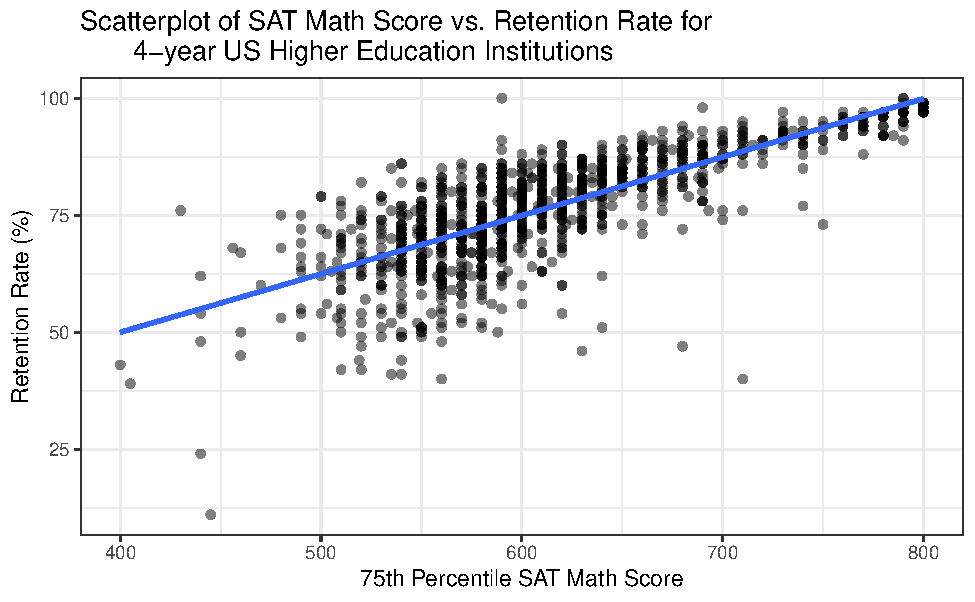
\includegraphics[width=0.7\linewidth]{13-A27-EDA-two-quantitative-corr_files/figure-latex/unnamed-chunk-2-1} \end{center}

\begin{enumerate}
\def\labelenumi{\arabic{enumi}.}
\tightlist
\item
  Describe the relationship between 75th percentile SAT Math score and retention rate.
\end{enumerate}

\vspace{1in}

\subsubsection*{Slope of the Least Squares Linear Regression Line}\label{slope-of-the-least-squares-linear-regression-line}
\addcontentsline{toc}{subsubsection}{Slope of the Least Squares Linear Regression Line}

There are three summary measures calculated from two quantitative variables: slope, correlation, and the coefficient of determination. We will first assess the slope of the least squares regression line between 75th percentile SAT Math score and retention rate.

\begin{itemize}
\item
  Enter \texttt{Retention} for response and \texttt{SATMath\_75} for explanatory in line 25
\item
  Highlight and run lines 25 -- 26 to fit the linear model.
\end{itemize}

\begin{Shaded}
\begin{Highlighting}[]
\CommentTok{\# Fit linear model: y \textasciitilde{} x}
\NormalTok{IPEDSLM }\OtherTok{\textless{}{-}} \FunctionTok{lm}\NormalTok{(Retention}\SpecialCharTok{\textasciitilde{}}\NormalTok{SATMath\_75, }\AttributeTok{data=}\NormalTok{IPEDS)}
\FunctionTok{round}\NormalTok{(}\FunctionTok{summary}\NormalTok{(IPEDSLM)}\SpecialCharTok{$}\NormalTok{coefficients,}\DecValTok{3}\NormalTok{) }\CommentTok{\# Display coefficient summary}
\end{Highlighting}
\end{Shaded}

\begin{verbatim}
#>             Estimate Std. Error t value Pr(>|t|)
#> (Intercept)    0.059      1.898   0.031    0.975
#> SATMath_75     0.125      0.003  40.485    0.000
\end{verbatim}

\begin{enumerate}
\def\labelenumi{\arabic{enumi}.}
\setcounter{enumi}{1}
\tightlist
\item
  Write out the least squares regression line using the summary statistics from the R output in context of the problem.
\end{enumerate}

\vspace{0.5in}

\textbf{Slope Interpretation}: An increase of one point in SAT Math 75th percentile score is associated with an increase in retention rate, on average, of 0.125 percentage points for 4-year higher education institutions.

\begin{enumerate}
\def\labelenumi{\arabic{enumi}.}
\setcounter{enumi}{2}
\tightlist
\item
  Predict the retention rate for a 4-year US higher education institution with a 75th percentile SAT Math score of 440.
\end{enumerate}

\vspace{0.4in}

\begin{enumerate}
\def\labelenumi{\arabic{enumi}.}
\setcounter{enumi}{3}
\tightlist
\item
  Calculate the residual for a 4-year US higher education institution with a 75th percentile SAT Math score of 440 and a retention rate of 24\%.
\end{enumerate}

\vspace{0.4in}

\subsubsection*{Correlation}\label{correlation-2}
\addcontentsline{toc}{subsubsection}{Correlation}

Correlation measures the strength and the direction of the linear relationship between two quantitative variables. The closer the value of correlation to \(+1\) or \(-1\), the stronger the linear relationship. Values close to zero indicate a very weak linear relationship between the two variables.

The following output creates a correlation matrix between several pairs of quantitative variables.

\begin{Shaded}
\begin{Highlighting}[]
\NormalTok{IPEDS }\SpecialCharTok{\%\textgreater{}\%}  \CommentTok{\# Data set pipes into}
  \FunctionTok{select}\NormalTok{(}\FunctionTok{c}\NormalTok{(}\StringTok{"Retention"}\NormalTok{, }\StringTok{"Cost\_InState"}\NormalTok{, }
           \StringTok{"Graduation\_Rate"}\NormalTok{, }\StringTok{"Salary"}\NormalTok{, }
           \StringTok{"SATMath\_75"}\NormalTok{, }\StringTok{"ACT\_75"}\NormalTok{)) }\SpecialCharTok{\%\textgreater{}\%}
  \FunctionTok{cor}\NormalTok{(}\AttributeTok{use=}\StringTok{"pairwise.complete.obs"}\NormalTok{) }\SpecialCharTok{\%\textgreater{}\%}
  \FunctionTok{round}\NormalTok{(}\DecValTok{3}\NormalTok{)}
\end{Highlighting}
\end{Shaded}

\begin{verbatim}
#>                 Retention Cost_InState Graduation_Rate Salary SATMath_75 ACT_75
#> Retention           1.000        0.388           0.832  0.698      0.767  0.768
#> Cost_InState        0.388        1.000           0.563  0.365      0.502  0.514
#> Graduation_Rate     0.832        0.563           1.000  0.683      0.817  0.833
#> Salary              0.698        0.365           0.683  1.000      0.747  0.706
#> SATMath_75          0.767        0.502           0.817  0.747      1.000  0.920
#> ACT_75              0.768        0.514           0.833  0.706      0.920  1.000
\end{verbatim}

\begin{enumerate}
\def\labelenumi{\arabic{enumi}.}
\setcounter{enumi}{4}
\tightlist
\item
  What is the value of correlation between SATMath\_75 and Retention?
\end{enumerate}

\vspace{0.3in}

\subsubsection*{Coefficient of determination (squared correlation)}\label{coefficient-of-determination-squared-correlation}
\addcontentsline{toc}{subsubsection}{Coefficient of determination (squared correlation)}

Another summary measure used to explain the linear relationship between two quantitative variables is the coefficient of determination (\(r^2\)). The coefficient of determination, \(r^2\), can also be used to describe the strength of the linear relationship between two quantitative variables. The value of \(r^2\) (a value between 0 and 1) represents the \textbf{proportion of variation in the response that is explained by the least squares line with the explanatory variable}. There are two ways to calculate the coefficient of determination:

~~~Square the correlation coefficient: \(r^2 = (r)^2\)

~~~Use the variances of the response and the residuals: \(r^2 = \dfrac{s_y^2 - s_{RES}^2}{s_y^2} = \dfrac{SST - SSE}{SST}\)

\begin{enumerate}
\def\labelenumi{\arabic{enumi}.}
\setcounter{enumi}{5}
\tightlist
\item
  Use the correlation, \(r\), found in question 5, to calculate the coefficient of determination between SATMath\_75 and Retention, \(r^2\).
\end{enumerate}

\vspace{.4in}

\begin{enumerate}
\def\labelenumi{\arabic{enumi}.}
\setcounter{enumi}{6}
\tightlist
\item
  The variance of the response variable, Retention in \$MM, is \(s_{Retention}^2 = 138.386\) \(\%^2\) and the variability in the residuals is \(s_{RES}^2 = 56.934\) \%\(^2\). Use these values to calculate the coefficient of determination.
\end{enumerate}

\vspace{1in}

In the next part of the activity we will explore what the coefficient of determination measures.

In the first scatterplot, we see the data plotted with a horizontal line. Note that the regression line in this plot has a slope of zero; this assumes there is no relationship between SATMath\_75 and Retention. The value of the y-intercept, 76.387, is the mean of the response variable when there is no relationship between the two variables. To find the sum of squares total (SST) we find the residual (\(residual = y - \hat{y}\)) for each response value from the horizontal line (from the value of 76.387). Each residual is squared and the sum of the squared values is calculated. The SST gives the \textbf{total variability in the response variable, Retention}.

\begin{center}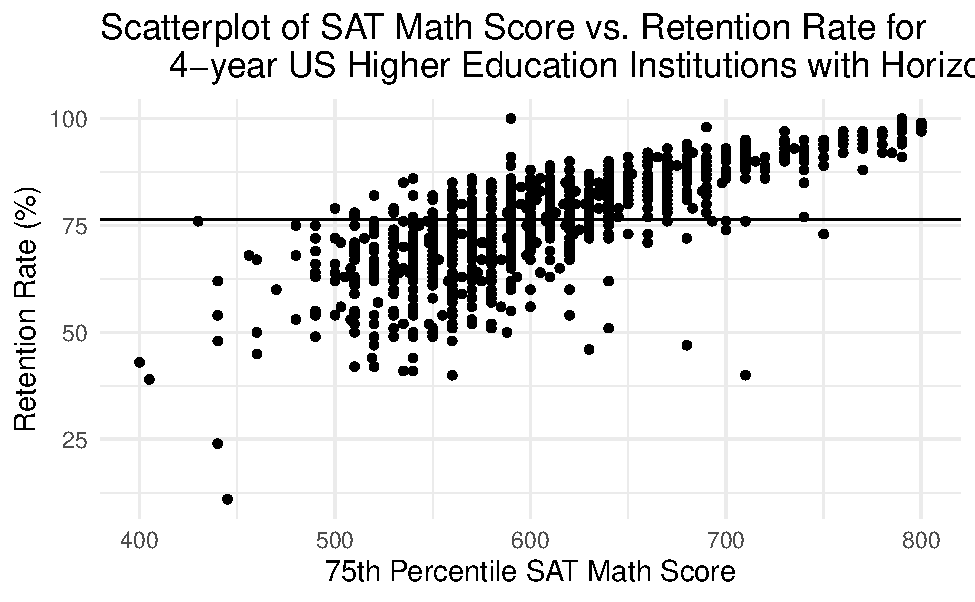
\includegraphics[width=0.7\linewidth]{13-A27-EDA-two-quantitative-corr_files/figure-latex/unnamed-chunk-5-1} \end{center}

The calculated value for the SST is 158451.8.

This next scatterplot, shows the plotted data with the best fit regression line. This is the line of best fit between budget and revenue and has the smallest sum of squares error (SSE). The SSE is calculated by finding the residual from each response value to the regression line. Each residual is squared and the sum of the squared values is calculated.

\begin{center}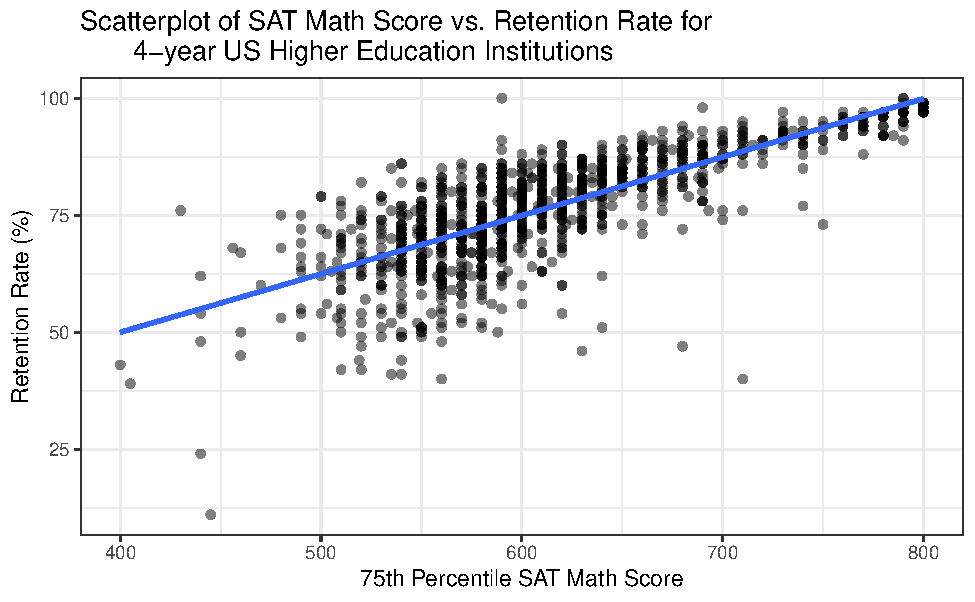
\includegraphics[width=0.7\linewidth]{13-A27-EDA-two-quantitative-corr_files/figure-latex/unnamed-chunk-6-1} \end{center}

The calculated value for the SSE is 65133.022.

\begin{enumerate}
\def\labelenumi{\arabic{enumi}.}
\setcounter{enumi}{7}
\tightlist
\item
  Calculate the value for \(r^2\) using the values for SST and SSE provided below each of the previous graphs.
\end{enumerate}

\vspace{0.8in}

\begin{enumerate}
\def\labelenumi{\arabic{enumi}.}
\setcounter{enumi}{8}
\tightlist
\item
  Write a sentence interpreting the coefficient of determination in context of the problem.
\end{enumerate}

\newpage

\subsubsection*{Multivariable plots}\label{multivariable-plots}
\addcontentsline{toc}{subsubsection}{Multivariable plots}

When adding another categorical predictor, we can add that variable as shape or color to the plot. In the following code we have added the variable \texttt{Sector}, whether the 4-year institution is public or private.

\begin{Shaded}
\begin{Highlighting}[]
\NormalTok{IPEDS }\SpecialCharTok{\%\textgreater{}\%} \CommentTok{\# Data sest pipes into...}
    \FunctionTok{ggplot}\NormalTok{(}\FunctionTok{aes}\NormalTok{(}\AttributeTok{x =}\NormalTok{ SATMath\_75, }\AttributeTok{y =}\NormalTok{ Retention, }\AttributeTok{shape =}\NormalTok{ Sector, }\AttributeTok{color=}\NormalTok{Sector))}\SpecialCharTok{+}  \CommentTok{\# Specify variables}
    \FunctionTok{geom\_point}\NormalTok{(}\AttributeTok{alpha=}\FloatTok{0.5}\NormalTok{) }\SpecialCharTok{+}  \CommentTok{\# Add scatterplot of points}
    \FunctionTok{labs}\NormalTok{(}\AttributeTok{x =} \StringTok{"75th Percentile SAT Math Score"}\NormalTok{,  }\CommentTok{\# Label x{-}axis}
       \AttributeTok{y =} \StringTok{"Retention Rate (\%)"}\NormalTok{,  }\CommentTok{\# Label y{-}axis}
       \AttributeTok{title =} \StringTok{"Scatterplot of SAT Math Score vs. Retention Rate for }
\StringTok{       4{-}year US Higher Education Institutions"}\NormalTok{) }\SpecialCharTok{+} 
    \CommentTok{\# Be sure to title your plots with the type of plot, observational units, variable(s)}
    \FunctionTok{geom\_smooth}\NormalTok{(}\AttributeTok{method =} \StringTok{"lm"}\NormalTok{, }\AttributeTok{se =} \ConstantTok{FALSE}\NormalTok{) }\SpecialCharTok{+} \CommentTok{\# Add regression line}
    \FunctionTok{scale\_color\_grey}\NormalTok{()}
\end{Highlighting}
\end{Shaded}

\begin{center}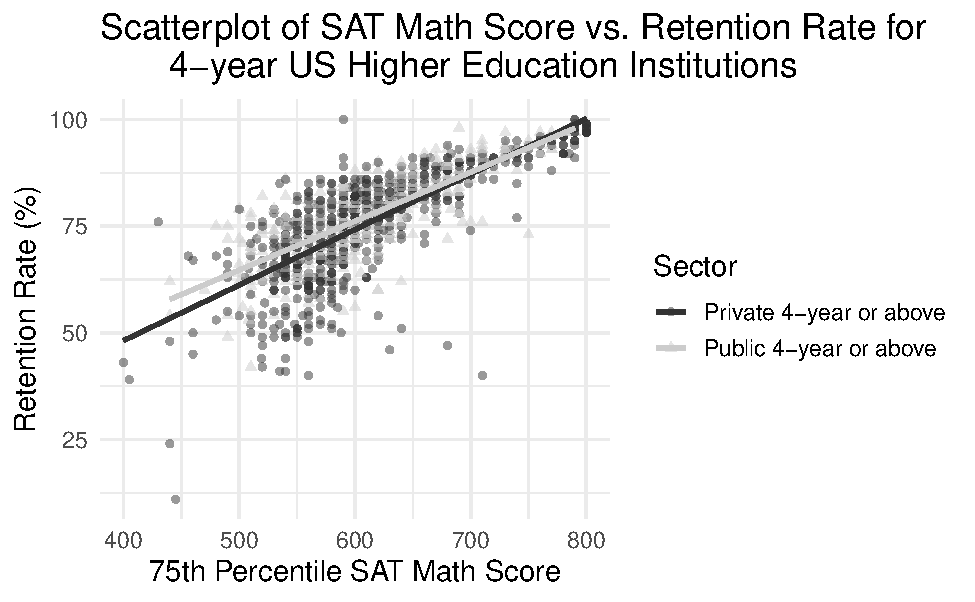
\includegraphics[width=0.7\linewidth]{13-A27-EDA-two-quantitative-corr_files/figure-latex/unnamed-chunk-7-1} \end{center}

\begin{enumerate}
\def\labelenumi{\arabic{enumi}.}
\setcounter{enumi}{9}
\tightlist
\item
  Does the relationship between 75th percentile SAT math score and retention rate of 4-year institutions change depending on the level of sector?
\end{enumerate}

\vspace{0.8in}

\newpage

\subsection{Take-home messages}\label{take-home-messages-6}

\begin{enumerate}
\def\labelenumi{\arabic{enumi}.}
\item
  The sign of correlation and the sign of the slope will always be the same. The closer the value of correlation is to \(-1\) or \(+1\), the stronger the linear relationship between the explanatory and the response variable.
\item
  The coefficient of determination multiplied by 100 (\(r^2 \times 100\)) measures the percent of variation in the response variable that is explained by the relationship with the explanatory variable. The closer the value of the coefficient of determination is to 100\%, the stronger the relationship.
\item
  We can use the line of regression to predict values of the response variable for values of the explanatory variable. Do not use values of the explanatory variable that are outside of the range of values in the data set to predict values of the response variable (reflect on why this is true.). This is called \textbf{extrapolation}.
\end{enumerate}

\subsection{Additional notes}\label{additional-notes-6}

Use this space to summarize your thoughts and take additional notes on today's activity and material covered.

\newpage

\section{Activity 28: Prediction of Crocodilian Body Size}\label{activity-28-prediction-of-crocodilian-body-size}

\setstretch{1}

\subsection{Learning outcomes}\label{learning-outcomes-9}

\begin{itemize}
\item
  Given a research question involving two quantitative variables, construct the null and alternative hypotheses
  in words and using appropriate statistical symbols.
\item
  Describe and perform a simulation-based hypothesis test for slope or correlation.
\item
  Interpret and evaluate a p-value for a simulation-based hypothesis test for a slope or correlation.
\item
  Use bootstrapping to find a confidence interval for the slope or correlation.
\item
  Interpret a confidence interval for a slope or correlation.
\end{itemize}

\subsection{Terminology review}\label{terminology-review-7}

In today's activity, we will use simulation-based methods for hypothesis tests and confidence intervals for a linear regression slope or correlation. Some terms covered in this activity are:

\begin{itemize}
\item
  Correlation
\item
  Slope
\item
  Regression line
\end{itemize}

To review these concepts, see Chapter 21 in the textbook.

\subsection{Crocodilian Body Size}\label{crocodilian-body-size}

Much research surrounds using measurements of animals to estimate body-size of extinct animals. Many challenges exist in making accurate estimates for extinct crocodilians. The term crocodilians refers to all members of the family Crocodylidae (``true'' crocodiles), family Alligatoridae (alligators and caimans) and family Gavialidae (gharial, Tomistoma). The researchers in this study (O'Brien 2019) state, ``Among extinct crocodilians and their precursors (e.g., suchians), several methods have been developed to predict body size from suites of hard-tissue proxies. Nevertheless, many have limited applications due to the disparity of some major suchian groups and biases in the fossil record. Here, we test the utility of head width (HW) as a broadly applicable body-size estimator in living and fossil suchians.'' Data were collected on 76 male and female individuals of different species. Is there evidence that head width (measured in cm) is a good predictor of total body length (measured in cm) for crocodilians?

\begin{itemize}
\item
  Download the R script file from D2L and upload to the RStudio server
\item
  Open the file and run lines 1 - 8 to load the dataset
\end{itemize}

\begin{Shaded}
\begin{Highlighting}[]
\CommentTok{\# Read in data set}
\NormalTok{croc }\OtherTok{\textless{}{-}} \FunctionTok{read.csv}\NormalTok{(}\StringTok{"https://math.montana.edu/courses/s216/data/Crocodylian\_headwidth.csv"}\NormalTok{)}
\NormalTok{croc }\OtherTok{\textless{}{-}}\NormalTok{ croc }\SpecialCharTok{\%\textgreater{}\%}
    \FunctionTok{na.omit}\NormalTok{()}
\end{Highlighting}
\end{Shaded}

To create a scatterplot to examine the relationship between head width and total body length we will use \texttt{HW\_cm} as the explanatory variable and \texttt{TL\_cm} as the response variable.

\begin{itemize}
\item
  Enter the name of the explanatory and response variable in line 14
\item
  Highlight and run lines 13 - 20
\end{itemize}

\newpage

\begin{Shaded}
\begin{Highlighting}[]
\NormalTok{croc }\SpecialCharTok{\%\textgreater{}\%} \CommentTok{\# Pipe data set into...}
\FunctionTok{ggplot}\NormalTok{(}\FunctionTok{aes}\NormalTok{(}\AttributeTok{x =}\NormalTok{ explanatory, }\AttributeTok{y =}\NormalTok{ response))}\SpecialCharTok{+}  \CommentTok{\# Specify variables}
  \FunctionTok{geom\_point}\NormalTok{(}\AttributeTok{alpha=}\FloatTok{0.5}\NormalTok{) }\SpecialCharTok{+}  \CommentTok{\# Add scatterplot of points}
  \FunctionTok{labs}\NormalTok{(}\AttributeTok{x =} \StringTok{"head width (cm)"}\NormalTok{,  }\CommentTok{\# Label x{-}axis}
       \AttributeTok{y =} \StringTok{"total length (cm)"}\NormalTok{,  }\CommentTok{\# Label y{-}axis}
       \AttributeTok{title =} \StringTok{"Scatterplot of Crocodilian Head Width vs. Total Length"}\NormalTok{) }\SpecialCharTok{+} 
    \CommentTok{\# Be sure to title your plots}
  \FunctionTok{geom\_smooth}\NormalTok{(}\AttributeTok{method =} \StringTok{"lm"}\NormalTok{, }\AttributeTok{se =} \ConstantTok{FALSE}\NormalTok{)  }\CommentTok{\# Add regression line}
\end{Highlighting}
\end{Shaded}

\begin{enumerate}
\def\labelenumi{\arabic{enumi}.}
\tightlist
\item
  Describe the features of the plot, addressing all four characteristics of a scatterplot.
\end{enumerate}

\vspace{1in}

~~~~~~~If you indicated there are potential outliers, which points are they?

\vspace{0.5in}

\subsubsection*{Hypotheses}\label{hypotheses}
\addcontentsline{toc}{subsubsection}{Hypotheses}

When analyzing two quantitative variables we can either test regression slope or correlation. In both cases, we are testing that there is a linear relationship between variables.

\begin{enumerate}
\def\labelenumi{\arabic{enumi}.}
\setcounter{enumi}{1}
\tightlist
\item
  Write the null hypothesis in words.
\end{enumerate}

\vspace{0.6in}

\begin{enumerate}
\def\labelenumi{\arabic{enumi}.}
\setcounter{enumi}{2}
\tightlist
\item
  Write the null hypothesis to test slope in notation.
\end{enumerate}

\vspace{0.3in}

\begin{enumerate}
\def\labelenumi{\arabic{enumi}.}
\setcounter{enumi}{3}
\tightlist
\item
  Write the null hypothesis to test correlation in notation.
\end{enumerate}

\vspace{0.3in}

\begin{enumerate}
\def\labelenumi{\arabic{enumi}.}
\setcounter{enumi}{4}
\tightlist
\item
  Write the alternative hypothesis in words.
\end{enumerate}

\vspace{0.6in}

\newpage

\subsubsection*{Summarize and visualize the data}\label{summarize-and-visualize-the-data-1}
\addcontentsline{toc}{subsubsection}{Summarize and visualize the data}

To create the linear model output and find the value of correlation for the linear relationship\ldots{}

\begin{itemize}
\item
  Enter the the name of the explanatory and response in line 25
\item
  Highlight and run lines 25 - 27
\end{itemize}

\begin{Shaded}
\begin{Highlighting}[]
\CommentTok{\#Linear model}
\NormalTok{lm.croc }\OtherTok{\textless{}{-}} \FunctionTok{lm}\NormalTok{(response}\SpecialCharTok{\textasciitilde{}}\NormalTok{explanatory, }\AttributeTok{data=}\NormalTok{croc) }\CommentTok{\#lm(response\textasciitilde{}explanatory)}
\FunctionTok{round}\NormalTok{(}\FunctionTok{summary}\NormalTok{(lm.croc)}\SpecialCharTok{$}\NormalTok{coefficients, }\DecValTok{5}\NormalTok{)}
\CommentTok{\#Correlation}
\FunctionTok{cor}\NormalTok{(croc}\SpecialCharTok{$}\NormalTok{HW\_cm, croc}\SpecialCharTok{$}\NormalTok{TL\_cm)}
\end{Highlighting}
\end{Shaded}

\begin{enumerate}
\def\labelenumi{\arabic{enumi}.}
\setcounter{enumi}{5}
\tightlist
\item
  Using the output from the evaluated R code, write the equation of the regression line in the context of the problem using appropriate statistical notation.
\end{enumerate}

\vspace{1in}

\begin{enumerate}
\def\labelenumi{\arabic{enumi}.}
\setcounter{enumi}{6}
\tightlist
\item
  Interpret the estimated slope in context of the problem.
\end{enumerate}

\vspace{1in}

\subsubsection*{Use statistical inferential methods to draw inferences from the data}\label{use-statistical-inferential-methods-to-draw-inferences-from-the-data-6}
\addcontentsline{toc}{subsubsection}{Use statistical inferential methods to draw inferences from the data}

In this activity, we will focus on using simulation-based methods for inference in regression.

\subsubsection*{Simulation-based hypothesis test}\label{simulation-based-hypothesis-test}
\addcontentsline{toc}{subsubsection}{Simulation-based hypothesis test}

Let's start by thinking about how one simulation would be created on the null distribution using cards. First, we would write the values for the response variable, total length, on each card. Next, we would shuffle these \(y\) values while keeping the \(x\) values (explanatory variable) in the same order. Then, find the line of regression for the shuffled \((x, y)\) pairs and calculate either the slope or correlation of the shuffled sample.

We will use the \texttt{regression\_test()} function in R (in the \texttt{catstats} package) to simulate the null distribution of shuffled slopes (or shuffled correlations) and compute a p-value. We will need to enter the response variable name and the explanatory variable name for the formula, the data set name (identified above as \texttt{croc}), the summary measure for the test (either slope or correlation), number of repetitions, the sample statistic (value of slope or correlation), and the direction of the alternative hypothesis.

The response variable name is \texttt{TL\_cm} and the explanatory variable name is \texttt{HW\_cm} for these data.

\begin{enumerate}
\def\labelenumi{\arabic{enumi}.}
\setcounter{enumi}{7}
\tightlist
\item
  What inputs should be entered for each of the following to create the simulation to test regression slope?
\end{enumerate}

\vspace{.5 mm}

\begin{itemize}
\tightlist
\item
  Direction (\texttt{"greater"}, \texttt{"less"}, or \texttt{"two-sided"}):
\end{itemize}

\vspace{.2in}

\begin{itemize}
\tightlist
\item
  Summary measure (choose \texttt{"slope"} or \texttt{"correlation"}):
\end{itemize}

\vspace{.2in}

\begin{itemize}
\tightlist
\item
  As extreme as (enter the value for the sample slope):
\end{itemize}

\vspace{0.2in}

\begin{itemize}
\tightlist
\item
  Number of repetitions:
\end{itemize}

\vspace{.2in}

Using the R script file for this activity\ldots{}

\begin{itemize}
\item
  Enter your answers for question 8 in place of the \texttt{xx}'s to produce the null distribution with 1000 simulations.
\item
  Highlight and run lines 32--37.
\end{itemize}

\begin{Shaded}
\begin{Highlighting}[]
\FunctionTok{regression\_test}\NormalTok{(TL\_cm}\SpecialCharTok{\textasciitilde{}}\NormalTok{HW\_cm, }\CommentTok{\# response \textasciitilde{} explanatory}
               \AttributeTok{data =}\NormalTok{ croc, }\CommentTok{\# Name of data set}
               \AttributeTok{direction =} \StringTok{"xx"}\NormalTok{, }\CommentTok{\# Sign in alternative ("greater", "less", "two{-}sided")}
               \AttributeTok{summary\_measure =} \StringTok{"xx"}\NormalTok{, }\CommentTok{\# "slope" or "correlation"}
               \AttributeTok{as\_extreme\_as =}\NormalTok{ xx, }\CommentTok{\# Observed slope or correlation}
               \AttributeTok{number\_repetitions =} \DecValTok{10000}\NormalTok{) }\CommentTok{\# Number of simulated samples for null distribution}
\end{Highlighting}
\end{Shaded}

\begin{enumerate}
\def\labelenumi{\arabic{enumi}.}
\setcounter{enumi}{8}
\item
  Report the p-value from the R output.
  \vspace{0.5in}
\item
  Suppose we wanted to complete the simulation test using correlation as the summary measure, instead of slope. Which two inputs in \#8 would need to be changed to test for correlation? What inputs should you use instead?
  \vspace{0.75in}
\item
  Change the inputs in lines 32--37 to test for correlation instead of slope. Highlight and run those lines, then report the new p-value of the test.
  \vspace{0.5in}
\item
  The p-values from the test of slope (\#9) and the test of correlation (\#11) should be similar. Explain why the two p-values should match. \emph{Hint: think about the relationship between slope and correlation!}
  \vspace{1in}
\end{enumerate}

\subsubsection*{Simulation-based confidence interval}\label{simulation-based-confidence-interval}
\addcontentsline{toc}{subsubsection}{Simulation-based confidence interval}

We will use the \texttt{regression\_bootstrap\_CI()} function in R (in the \texttt{catstats} package) to simulate the bootstrap distribution of sample slopes (or sample correlations) and calculate a confidence interval.

\begin{itemize}
\item
  Fill in the missing values in the provided R script file to find a 95\% confidence interval for slope.
\item
  Highlight and run lines 42--46.
\end{itemize}

\begin{Shaded}
\begin{Highlighting}[]
\FunctionTok{regression\_bootstrap\_CI}\NormalTok{(response}\SpecialCharTok{\textasciitilde{}}\NormalTok{explanatory, }\CommentTok{\# response \textasciitilde{} explanatory}
   \AttributeTok{data =}\NormalTok{ croc, }\CommentTok{\# Name of data set}
   \AttributeTok{confidence\_level =}\NormalTok{ xx, }\CommentTok{\# Confidence level as decimal}
   \AttributeTok{summary\_measure =} \StringTok{"xx"}\NormalTok{, }\CommentTok{\# Slope or correlation}
   \AttributeTok{number\_repetitions =} \DecValTok{10000}\NormalTok{) }\CommentTok{\# Number of simulated samples for bootstrap distribution}
\end{Highlighting}
\end{Shaded}

\begin{enumerate}
\def\labelenumi{\arabic{enumi}.}
\setcounter{enumi}{12}
\item
  Report the bootstrap 95\% confidence interval in interval notation.\\
  \vspace{0.5in}
\item
  Interpret the interval in question 14 in context of the problem. \emph{Hint: use the interpretation of slope in your confidence interval interpretation.}
\end{enumerate}

\vspace{0.8in}

\subsubsection*{Communicate the results and answer the research question}\label{communicate-the-results-and-answer-the-research-question-1}
\addcontentsline{toc}{subsubsection}{Communicate the results and answer the research question}

\begin{enumerate}
\def\labelenumi{\arabic{enumi}.}
\setcounter{enumi}{14}
\tightlist
\item
  Based on the p-value and confidence interval, write a conclusion in context of the problem.
\end{enumerate}

\vspace{.8in}

\subsection{Take-home messages}\label{take-home-messages-7}

\begin{enumerate}
\def\labelenumi{\arabic{enumi}.}
\item
  The p-value for a test for correlation should be approximately the same as the p-value for the test of slope. In the simulation test, we just change the statistic type from slope to correlation and use the appropriate sample statistic value.
\item
  To interpret a confidence interval for the slope, think about how to interpret the sample slope and use that information in the confidence interval interpretation for slope.
\item
  To create one simulated sample on the null distribution when testing for a relationship between two quantitative variables, hold the \(x\) values constant and shuffle the \(y\) values to new \(x\) values. Find the regression line for the shuffled data and plot the slope or the correlation for the shuffled data.
\item
  To create one simulated sample on the bootstrap distribution when assessing two quantitative variables, label \(n\) cards with the original (response, explanatory) values. Randomly draw with replacement \(n\) times. Find the regression line for the resampled data and plot the resampled slope or correlation.
\end{enumerate}

\subsection{Additional notes}\label{additional-notes-7}

Use this space to summarize your thoughts and take additional notes on today's activity and material covered.

\newpage

\section{Activity 29: Golf Driving Distance}\label{activity-29-golf-driving-distance}

\setstretch{1}

\subsection{Learning outcomes}\label{learning-outcomes-10}

\begin{itemize}
\item
  Given a research question involving two quantitative variables, construct the null and alternative hypotheses
  in words and using appropriate statistical symbols.
\item
  Assess the conditions to use the normal distribution model for a slope.
\item
  Find the T test statistic (T-score) for a slope based off of \texttt{lm()} output in R.
\item
  Find, interpret, and evaluate the p-value for a theory-based hypothesis test for a slope.
\item
  Create and interpret a theory-based confidence interval for a slope.
\item
  Use a confidence interval to determine the conclusion of a hypothesis test.
\end{itemize}

\subsection{Terminology review}\label{terminology-review-8}

In this week's in-class activity, we will use theory-based methods for hypothesis tests and confidence intervals for a linear regression slope. Some terms covered in this activity are:

\begin{itemize}
\item
  Slope
\item
  Regression line
\end{itemize}

To review these concepts, see Chapter 21 in the textbook.

\subsection{Golf driving distance}\label{golf-driving-distance}

In golf the goal is to complete a hole with as few strokes as possible. A long driving distance to start a hole can help minimize the strokes necessary to complete the hole, as long as that drive stays on the fairway. Data were collected on 354 PGA and LPGA players in 2008 ({``Average Driving Distance and Fairway Accuracy''} 2008). For each player, the average driving distance (yards), fairway accuracy (percentage), and sex was measured. Use these data to assess, ``Does a professional golfer give up accuracy when they hit the ball farther?''

\begin{itemize}
\tightlist
\item
  Download the R script file from D2L and open in the RStudio server
\end{itemize}

\begin{Shaded}
\begin{Highlighting}[]
\CommentTok{\# Read in data set}
\NormalTok{golf }\OtherTok{\textless{}{-}} \FunctionTok{read.csv}\NormalTok{(}\StringTok{"https://math.montana.edu/courses/s216/data/golf.csv"}\NormalTok{)}
\end{Highlighting}
\end{Shaded}

\subsubsection*{Plot review.}\label{plot-review.}
\addcontentsline{toc}{subsubsection}{Plot review.}

To create a scatterplot showing the relationship between the driving distance and percent accuracy for professional golfers:

\begin{itemize}
\item
  Enter the name of the explanatory and response in line 10
\item
  Highlight and run lines 1 - 16
\end{itemize}

\begin{Shaded}
\begin{Highlighting}[]
\NormalTok{golf }\SpecialCharTok{\%\textgreater{}\%} \CommentTok{\# Pipe data set into...}
\FunctionTok{ggplot}\NormalTok{(}\FunctionTok{aes}\NormalTok{(}\AttributeTok{x =}\NormalTok{ explanatory, }\AttributeTok{y =}\NormalTok{ response))}\SpecialCharTok{+}  \CommentTok{\# Specify variables}
  \FunctionTok{geom\_point}\NormalTok{(}\AttributeTok{alpha=}\FloatTok{0.5}\NormalTok{) }\SpecialCharTok{+}  \CommentTok{\# Add scatterplot of points}
  \FunctionTok{labs}\NormalTok{(}\AttributeTok{x =} \StringTok{"Driving Distance (yards)"}\NormalTok{,  }\CommentTok{\# Label x{-}axis}
       \AttributeTok{y =} \StringTok{"Percent Accuracy"}\NormalTok{,  }\CommentTok{\# Label y{-}axis}
       \AttributeTok{title =} \StringTok{"Scatterplot of Driving Distance by Percent Accuracy}
\StringTok{       for Professional Golfers"}\NormalTok{) }\SpecialCharTok{+} 
               \CommentTok{\# Be sure to tile your plots}
  \FunctionTok{geom\_smooth}\NormalTok{(}\AttributeTok{method =} \StringTok{"lm"}\NormalTok{, }\AttributeTok{se =} \ConstantTok{FALSE}\NormalTok{)  }\CommentTok{\# Add regression line}
\end{Highlighting}
\end{Shaded}

\subsubsection*{Conditions for the least squares line}\label{conditions-for-the-least-squares-line}
\addcontentsline{toc}{subsubsection}{Conditions for the least squares line}

When performing inference on a least squares line, the follow conditions are generally required:

\begin{itemize}
\tightlist
\item
  \emph{Independent observations} (for both simulation-based and theory-based methods): individual data points must be independent.

  \begin{itemize}
  \tightlist
  \item
    Check this assumption by investigating the sampling method and determining if the observational units are related in any way.
  \end{itemize}
\item
  \emph{Linearity} (for both simulation-based and theory-based methods): the data should follow a linear trend.

  \begin{itemize}
  \tightlist
  \item
    Check this assumption by examining the scatterplot of the two variables, and a scatterplot of the residuals (on the \(y\)-axis) versus the fitted values (on the \(x\)-axis). The pattern in the residual plot should display a horizontal line.
  \end{itemize}
\item
  \emph{Constant variability} (for theory-based methods only): the variability of points around the least squares line remains roughly constant

  \begin{itemize}
  \tightlist
  \item
    Check this assumption by examining a scatterplot of the residuals (on the \(y\)-axis) versus the fitted values (on the \(x\)-axis). The variability in the residuals around zero should be approximately the same for all fitted values.
  \end{itemize}
\item
  \emph{Nearly normal residuals} (for theory-based methods only: residuals must be nearly normal.

  \begin{itemize}
  \tightlist
  \item
    Check this assumption by examining a histogram of the residuals, which should appear approximately normal.
  \end{itemize}
\end{itemize}

The scatterplot generated earlier and the residual plots shown below will be used to assess these conditions for approximating the data with the \(t\)-distribution.

\begin{center}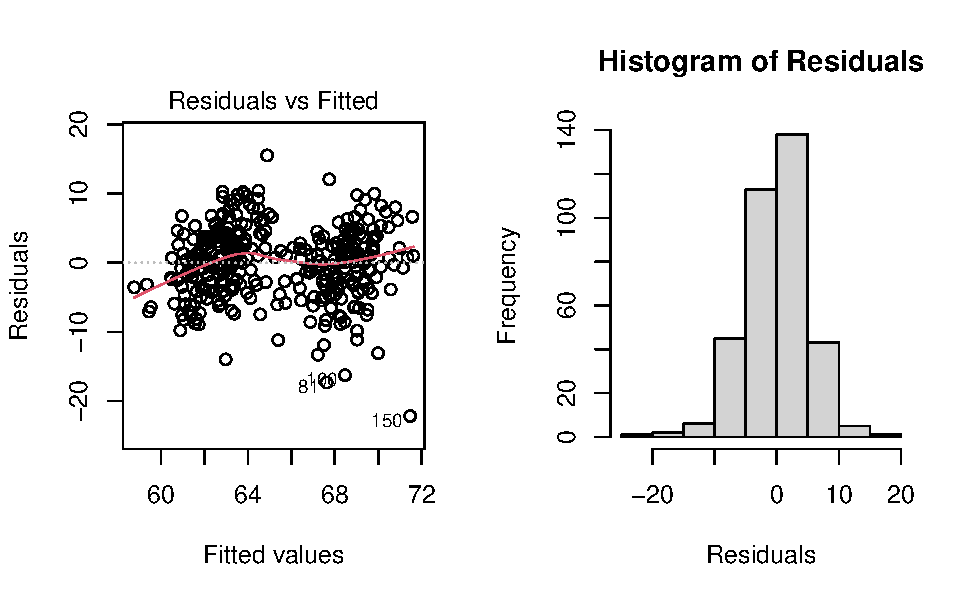
\includegraphics[width=0.7\linewidth]{13-A29-regression-theory_files/figure-latex/unnamed-chunk-3-1} \end{center}

\begin{enumerate}
\def\labelenumi{\arabic{enumi}.}
\tightlist
\item
  Are the conditions met to use the \(t\)-distribution to approximate the sampling distribution of the standardized statistic? Justify your answer.
\end{enumerate}

\vspace{3in}

\subsubsection*{Ask a research question}\label{ask-a-research-question-2}
\addcontentsline{toc}{subsubsection}{Ask a research question}

\begin{enumerate}
\def\labelenumi{\arabic{enumi}.}
\setcounter{enumi}{1}
\tightlist
\item
  Write out the null hypothesis in words to test the slope.
\end{enumerate}

\vspace{1in}

\begin{enumerate}
\def\labelenumi{\arabic{enumi}.}
\setcounter{enumi}{2}
\tightlist
\item
  Using the research question, write the alternative hypothesis in notation to test the slope.
\end{enumerate}

\vspace{0.4in}

\subsubsection*{Summarize and visualize the data}\label{summarize-and-visualize-the-data-2}
\addcontentsline{toc}{subsubsection}{Summarize and visualize the data}

The linear model output for this study is shown below.

\begin{Shaded}
\begin{Highlighting}[]
\NormalTok{lm.golf }\OtherTok{\textless{}{-}} \FunctionTok{lm}\NormalTok{(Percent\_Accuracy}\SpecialCharTok{\textasciitilde{}}\NormalTok{Driving\_Distance, }\AttributeTok{data=}\NormalTok{golf) }\CommentTok{\# lm(response\textasciitilde{}explanatory)}
\FunctionTok{round}\NormalTok{(}\FunctionTok{summary}\NormalTok{(lm.golf)}\SpecialCharTok{$}\NormalTok{coefficients, }\DecValTok{3}\NormalTok{)}
\end{Highlighting}
\end{Shaded}

\begin{verbatim}
#>                  Estimate Std. Error t value Pr(>|t|)
#> (Intercept)       103.586      3.329  31.119        0
#> Driving_Distance   -0.142      0.012 -11.553        0
\end{verbatim}

\begin{enumerate}
\def\labelenumi{\arabic{enumi}.}
\setcounter{enumi}{3}
\tightlist
\item
  Report the summary statistic (sample slope) for the linear relationship between driving distance and percent accuracy of golfers. Use proper notation.
\end{enumerate}

\vspace{0.3in}

\subsubsection*{Use statistical inferential methods to draw inferences from the data}\label{use-statistical-inferential-methods-to-draw-inferences-from-the-data-7}
\addcontentsline{toc}{subsubsection}{Use statistical inferential methods to draw inferences from the data}

\paragraph*{Hypothesis test}\label{hypothesis-test-2}
\addcontentsline{toc}{paragraph}{Hypothesis test}

To find the value of the standardized statistic to test the slope we will use,

\[
T = \frac{\mbox{slope estimate}-null value}{SE} = \frac{b_1-0}{SE(b_1)}.
\]

We will use the linear model R output above to get the estimate for slope and the standard error of the slope.

\begin{enumerate}
\def\labelenumi{\arabic{enumi}.}
\setcounter{enumi}{4}
\tightlist
\item
  Calculate the standardized statistic for slope. Identify where this calculated value is in the linear model R output.
\end{enumerate}

\vspace{0.7in}

\begin{enumerate}
\def\labelenumi{\arabic{enumi}.}
\setcounter{enumi}{5}
\tightlist
\item
  The p-value in the linear model R output is the two-sided p-value for the test of significance for slope. Report the p-value to answer the research question.
\end{enumerate}

\vspace{0.5in}

\begin{enumerate}
\def\labelenumi{\arabic{enumi}.}
\setcounter{enumi}{6}
\tightlist
\item
  Based on the p-value, how much evidence is there against the null hypothesis?
\end{enumerate}

\vspace{0.5in}

\paragraph*{Confidence interval}\label{confidence-interval-5}
\addcontentsline{toc}{paragraph}{Confidence interval}

Recall that a confidence interval is calculated by adding and subtracting the margin of error to the point estimate.\\
\[\mbox{point estimate}\pm t^*\times SE(\mbox{estimate}).\]
When the point estimate is a regression slope, this formula becomes
\[b_1 \pm t^* \times SE(b_1).\]

The \(t^*\) multiplier comes from a \(t\)-distribution with \(n-2\) degrees of freedom. The sample size for this study is 354 so we will use the degrees of freedom 352 (\(n-2\)).

\begin{itemize}
\item
  Enter the percentile needed to find the multiplier for a 95\% confidence interval for xx
\item
  Enter the degrees of freedom for yy
\item
  Highlight and run line 33
\end{itemize}

\begin{Shaded}
\begin{Highlighting}[]
\FunctionTok{qt}\NormalTok{(xx, yy, }\AttributeTok{lower.tail =} \ConstantTok{TRUE}\NormalTok{) }\CommentTok{\# 95\% t* multiplier }
\end{Highlighting}
\end{Shaded}

\begin{enumerate}
\def\labelenumi{\arabic{enumi}.}
\setcounter{enumi}{7}
\item
  Calculate the 95\% confidence interval for the true slope.
  \vspace{0.8in}
\item
  Interpret the 95\% confidence interval in context of the problem.
\end{enumerate}

\vspace{.8in}

\subsubsection*{Communicate the results and answer the research question}\label{communicate-the-results-and-answer-the-research-question-2}
\addcontentsline{toc}{subsubsection}{Communicate the results and answer the research question}

\begin{enumerate}
\def\labelenumi{\arabic{enumi}.}
\setcounter{enumi}{9}
\tightlist
\item
  Write a conclusion to answer the research question in context of the problem.
\end{enumerate}

\vspace{.8in}

\subsection*{Multivariable plots}\label{multivariable-plots-1}
\addcontentsline{toc}{subsection}{Multivariable plots}

Another variable that may affect the percent accuracy is the which league the golfer is part of. We will look at how this variable may change the relationship between driving distance and percent accuracy.

\begin{Shaded}
\begin{Highlighting}[]
\NormalTok{golf }\SpecialCharTok{\%\textgreater{}\%}
  \FunctionTok{ggplot}\NormalTok{(}\FunctionTok{aes}\NormalTok{(}\AttributeTok{x =}\NormalTok{ Driving\_Distance, }\AttributeTok{y =}\NormalTok{ Percent\_Accuracy, }\AttributeTok{color=}\NormalTok{League))}\SpecialCharTok{+}  \CommentTok{\# Specify variables}
  \FunctionTok{geom\_point}\NormalTok{(}\FunctionTok{aes}\NormalTok{(}\AttributeTok{shape =}\NormalTok{ League), }\AttributeTok{size =} \DecValTok{2}\NormalTok{, }\AttributeTok{alpha=}\FloatTok{0.5}\NormalTok{) }\SpecialCharTok{+}  \CommentTok{\# Add scatterplot of points}
  \FunctionTok{labs}\NormalTok{(}\AttributeTok{x =} \StringTok{"Driving Distance (yards)"}\NormalTok{,  }\CommentTok{\# Label x{-}axis}
       \AttributeTok{y =} \StringTok{"Percent Accuracy"}\NormalTok{,  }\CommentTok{\# Label y{-}axis}
       \AttributeTok{color =} \StringTok{"League"}\NormalTok{, }\AttributeTok{shape =} \StringTok{"League"}\NormalTok{,}
       \AttributeTok{title =} \StringTok{"Scatterplot of Golf Driving Distance and Percent }
\StringTok{       Accuracy by League for Professional Golfers"}\NormalTok{) }\SpecialCharTok{+} \CommentTok{\# Be sure to title your plots}
  \FunctionTok{geom\_smooth}\NormalTok{(}\AttributeTok{method =} \StringTok{"lm"}\NormalTok{, }\AttributeTok{se =} \ConstantTok{FALSE}\NormalTok{) }\SpecialCharTok{+} \CommentTok{\# Add regression line}
    \FunctionTok{scale\_color\_grey}\NormalTok{()}
\end{Highlighting}
\end{Shaded}

\begin{center}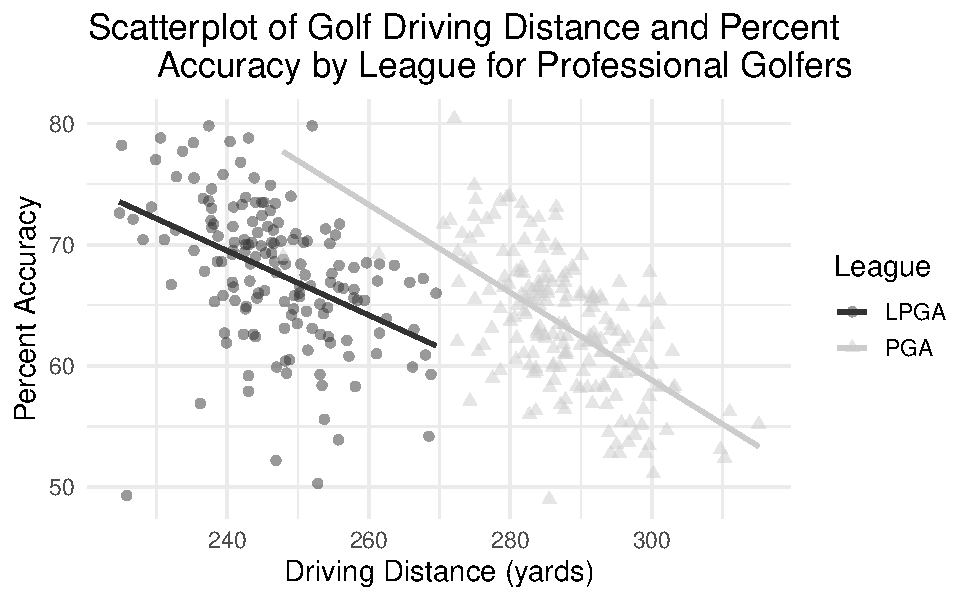
\includegraphics[width=0.6\linewidth]{13-A29-regression-theory_files/figure-latex/unnamed-chunk-6-1} \end{center}

\begin{enumerate}
\def\labelenumi{\arabic{enumi}.}
\setcounter{enumi}{10}
\item
  Does the association between driving distance and percent accuracy change depending on which league the golfer is a part of? Explain your answer.\\
  \vspace{1in}
\item
  Explain the association between league and each of the other two variables. Use the following plots in addition to the scatterplot from Q9 to explain your answer.
\end{enumerate}

\begin{center}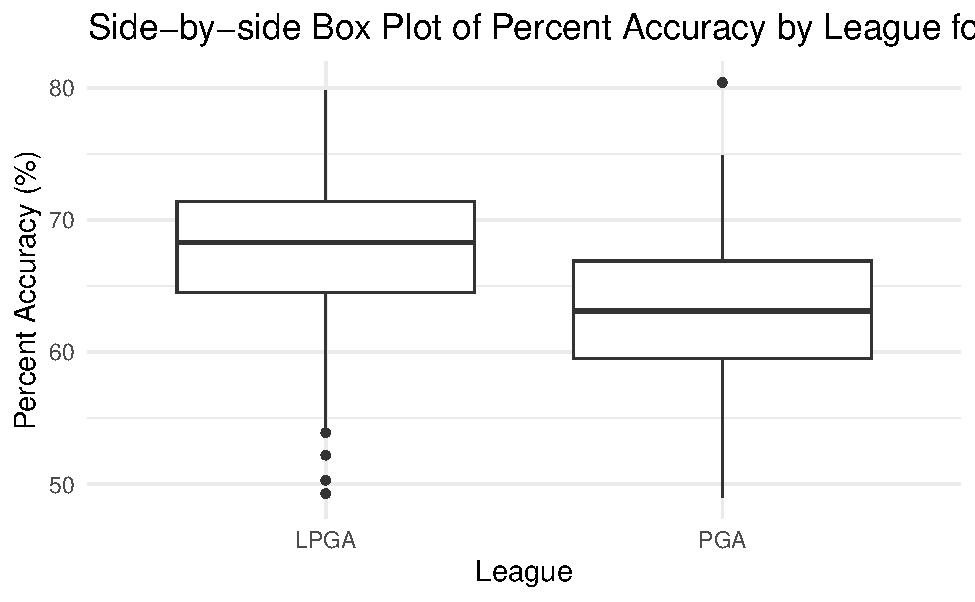
\includegraphics[width=0.7\linewidth]{13-A29-regression-theory_files/figure-latex/unnamed-chunk-7-1} \end{center}

\begin{center}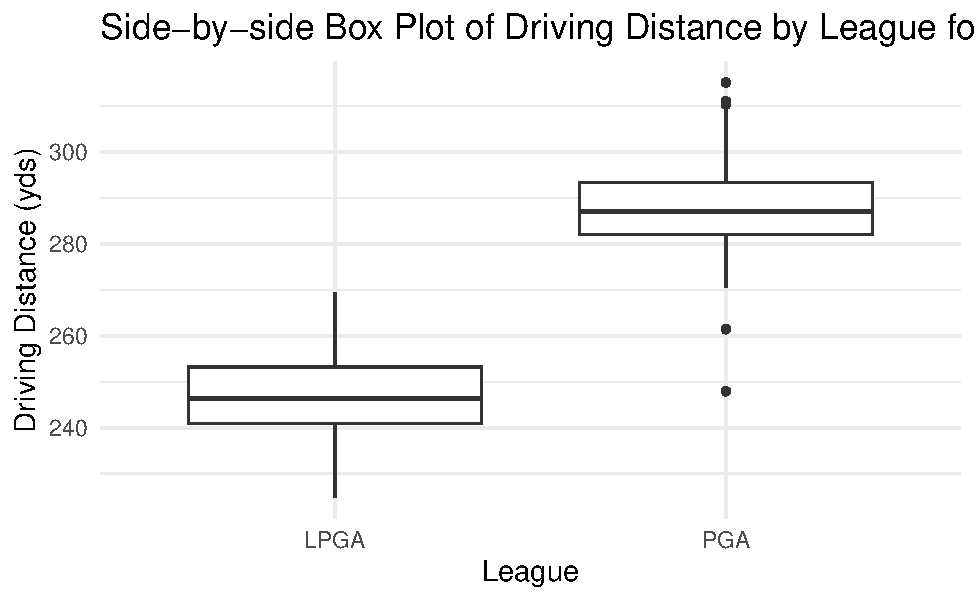
\includegraphics[width=0.7\linewidth]{13-A29-regression-theory_files/figure-latex/unnamed-chunk-8-1} \end{center}

\vspace{0.8in}

\subsection{Take-home messages}\label{take-home-messages-8}

\begin{enumerate}
\def\labelenumi{\arabic{enumi}.}
\item
  To check the validity conditions for using theory-based methods we must use the residual diagnostic plots to check for normality of residuals and constant variability, and the scatterplot to check for linearity.
\item
  To interpret a confidence interval for the slope, think about how to interpret the sample slope and use that information in the confidence interval interpretation for slope.
\item
  Use the explanatory variable row in the linear model R output to obtain the slope estimate (\texttt{estimate} column) and standard error of the slope (\texttt{Std.\ Error} column) to calculate the standardized slope, or T-score. The calculated T-score should match the \texttt{t\ value} column in the explanatory variable row. The standardized slope tells the number of standard errors the observed slope is above or below 0.
\item
  The explanatory variable row in the linear model R output provides a \textbf{two-sided} p-value under the \texttt{Pr(\textgreater{}\textbar{}t\textbar{})} column.
\item
  The standardized slope is compared to a \(t\)-distribution with \(n-2\) degrees of freedom in order to obtain a p-value. The \(t\)-distribution with \(n-2\) degrees of freedom is also used to find the appropriate multiplier for a given confidence level.
\end{enumerate}

\subsection{Additional notes}\label{additional-notes-8}

Use this space to summarize your thoughts and take additional notes on this week's activity and material covered.

\newpage

\section{Module 13 Lab: Big Mac Index}\label{module-13-lab-big-mac-index}

\setstretch{1}

\subsection{Learning outcomes}\label{learning-outcomes-11}

\begin{itemize}
\item
  Given a research question involving two quantitative variables, construct the null and alternative hypotheses
  in words and using appropriate statistical symbols.
\item
  Assess the conditions to determine in theory or simulation-based methods should be used.
\item
  Find, interpret, and evaluate the p-value for a hypothesis test for a slope or correlation.
\item
  Create and interpret a confidence interval for a slope or correlation.
\end{itemize}

\subsection{Big Mac Index}\label{big-mac-index}

Can the relative cost of a Big Mac across different countries be used to predict the Gross Domestic Product (GDP) per person for that country? The log GDP per person and the adjusted dollar equivalent to purchase a Big Mac was found on a random sample of 55 countries in January of 2022. The cost of a Big Mac in each country was adjusted to US dollars based on current exchange rates. Is there evidence of a positive relationship between Big Mac cost (\texttt{dollar\_price}) and the log GDP per person (\texttt{log\_GDP})?

\begin{itemize}
\item
  Upload and open the R script file for Week 13 lab.
\item
  Upload the csv file, \texttt{big\_mac\_adjusted\_index\_S22.csv}.
\item
  Enter the name of the data set for datasetname in the R script file in line 9.
\item
  Highlight and run lines 1--9 to load the data.
\end{itemize}

\begin{Shaded}
\begin{Highlighting}[]
\CommentTok{\# Read in data set }
\NormalTok{mac }\OtherTok{\textless{}{-}} \FunctionTok{read.csv}\NormalTok{(}\StringTok{"datasetname"}\NormalTok{)}
\end{Highlighting}
\end{Shaded}

\subsubsection*{Summarize and visualize the data}\label{summarize-and-visualize-the-data-3}
\addcontentsline{toc}{subsubsection}{Summarize and visualize the data}

\begin{itemize}
\tightlist
\item
  To find the correlation between the variables, \texttt{log\_GDP} and \texttt{dollar\_price} highlight and run lines 13--16 in the R script file.
\end{itemize}

\begin{Shaded}
\begin{Highlighting}[]
\NormalTok{mac }\SpecialCharTok{\%\textgreater{}\%} 
  \FunctionTok{select}\NormalTok{(}\FunctionTok{c}\NormalTok{(}\StringTok{"log\_GDP"}\NormalTok{, }\StringTok{"dollar\_price"}\NormalTok{)) }\SpecialCharTok{\%\textgreater{}\%}
  \FunctionTok{cor}\NormalTok{(}\AttributeTok{use=}\StringTok{"pairwise.complete.obs"}\NormalTok{) }\SpecialCharTok{\%\textgreater{}\%}
  \FunctionTok{round}\NormalTok{(}\DecValTok{3}\NormalTok{)}
\end{Highlighting}
\end{Shaded}

\begin{enumerate}
\def\labelenumi{\arabic{enumi}.}
\item
  Report the value of correlation between the variables.
  \vspace{0.2in}
\item
  \textbf{Calculate the value of the coefficient of determination between \texttt{log\_GDP} and \texttt{dollar\_price}.}
  \vspace{0.4in}
\item
  Interpret the value of the coefficient of determination in context of the problem.
  \vspace{0.6in}
\end{enumerate}

In the next part of the activity we will assess the linear model between Big Mac cost and log GDP.

\begin{itemize}
\item
  Enter the variable \texttt{log\_GDP} for \texttt{response} and the variable \texttt{dollar\_price} for \texttt{explanatory} in line 22.
\item
  Highlight and run lines 22--23 to get the linear model output.
\end{itemize}

\begin{Shaded}
\begin{Highlighting}[]
\CommentTok{\# Fit linear model: y \textasciitilde{} x}
\NormalTok{bigmacLM }\OtherTok{\textless{}{-}} \FunctionTok{lm}\NormalTok{(response}\SpecialCharTok{\textasciitilde{}}\NormalTok{explanatory, }\AttributeTok{data=}\NormalTok{mac)}
\FunctionTok{round}\NormalTok{(}\FunctionTok{summary}\NormalTok{(bigmacLM)}\SpecialCharTok{$}\NormalTok{coefficients,}\DecValTok{3}\NormalTok{) }\CommentTok{\# Display coefficient summary}
\end{Highlighting}
\end{Shaded}

\begin{enumerate}
\def\labelenumi{\arabic{enumi}.}
\setcounter{enumi}{3}
\tightlist
\item
  Give the value of the slope of the regression line. Interpret this value in context of the problem.
  \vspace{0.6in}
\end{enumerate}

\subsubsection*{Conditions for the least squares line}\label{conditions-for-the-least-squares-line-1}
\addcontentsline{toc}{subsubsection}{Conditions for the least squares line}

\begin{enumerate}
\def\labelenumi{\arabic{enumi}.}
\setcounter{enumi}{4}
\tightlist
\item
  Is there independence between the responses for the observational units? Justify your answer.
\end{enumerate}

\vspace{0.3in}

\begin{itemize}
\tightlist
\item
  Highlight and run lines 28--33 to create the scatterplot to check for linearity.
\end{itemize}

\begin{Shaded}
\begin{Highlighting}[]
\CommentTok{\#Scatterplot}
\NormalTok{mac }\SpecialCharTok{\%\textgreater{}\%} \CommentTok{\# Pipe data set into...}
  \FunctionTok{ggplot}\NormalTok{(}\FunctionTok{aes}\NormalTok{(}\AttributeTok{x =}\NormalTok{ dollar\_price, }\AttributeTok{y =}\NormalTok{ log\_GDP))}\SpecialCharTok{+}  \CommentTok{\# Specify variables}
  \FunctionTok{geom\_point}\NormalTok{(}\AttributeTok{alpha=}\FloatTok{0.5}\NormalTok{) }\SpecialCharTok{+}  \CommentTok{\# Add scatterplot of points}
  \FunctionTok{labs}\NormalTok{(}\AttributeTok{x =} \StringTok{"Big Mac Cost"}\NormalTok{,  }\CommentTok{\# Label x{-}axis}
       \AttributeTok{y =} \StringTok{"log GDP"}\NormalTok{,  }\CommentTok{\# Label y{-}axis}
       \AttributeTok{title =} \StringTok{"Scatterplot of Big Mac Cost vs. log GDP per person}
\StringTok{       for Countries in 2022"}\NormalTok{) }\SpecialCharTok{+}  \CommentTok{\# Be sure to tile your plots}
  \FunctionTok{geom\_smooth}\NormalTok{(}\AttributeTok{method =} \StringTok{"lm"}\NormalTok{, }\AttributeTok{se =} \ConstantTok{FALSE}\NormalTok{)  }\CommentTok{\# Add regression line}
\end{Highlighting}
\end{Shaded}

\begin{enumerate}
\def\labelenumi{\arabic{enumi}.}
\setcounter{enumi}{5}
\tightlist
\item
  Is the linearity condition met to use regression methods to analyze the data? Justify your answer.
\end{enumerate}

\vspace{0.3in}

\begin{itemize}
\tightlist
\item
  Highlight and run lines 38--42 to produce the diagnostic plots needed to assess conditions to use theory-based methods.
\end{itemize}

\begin{Shaded}
\begin{Highlighting}[]
\CommentTok{\#Diagnostic plots}
\NormalTok{bigmacLM }\OtherTok{\textless{}{-}} \FunctionTok{lm}\NormalTok{(log\_GDP}\SpecialCharTok{\textasciitilde{}}\NormalTok{dollar\_price, }\AttributeTok{data =}\NormalTok{ mac) }\CommentTok{\# Fit linear regression model}
\FunctionTok{par}\NormalTok{(}\AttributeTok{mfrow=}\FunctionTok{c}\NormalTok{(}\DecValTok{1}\NormalTok{,}\DecValTok{2}\NormalTok{)) }\CommentTok{\# Set graphics parameters to plot 2 plots in 1 row}
\FunctionTok{plot}\NormalTok{(bigmacLM, }\AttributeTok{which=}\DecValTok{1}\NormalTok{) }\CommentTok{\# Residual vs fitted values}
\FunctionTok{hist}\NormalTok{(bigmacLM}\SpecialCharTok{$}\NormalTok{resid, }\AttributeTok{xlab=}\StringTok{"Residuals"}\NormalTok{, }\AttributeTok{ylab=}\StringTok{"Frequency"}\NormalTok{,}
     \AttributeTok{main =} \StringTok{"Histogram of Residuals"}\NormalTok{) }\CommentTok{\# Histogram of residuals}
\end{Highlighting}
\end{Shaded}

\begin{enumerate}
\def\labelenumi{\arabic{enumi}.}
\setcounter{enumi}{6}
\tightlist
\item
  \textbf{Are the conditions met to use the \(t\)-distribution to approximate the sampling distribution of the standardized statistic? Justify your answer.}
\end{enumerate}

\vspace{1.5in}

\newpage

\subsubsection*{Ask a research question}\label{ask-a-research-question-3}
\addcontentsline{toc}{subsubsection}{Ask a research question}

\begin{enumerate}
\def\labelenumi{\arabic{enumi}.}
\setcounter{enumi}{7}
\tightlist
\item
  Write out the null and alternative hypotheses in notation to test \emph{correlation} between Big Mac cost and country GDP.
\end{enumerate}

\vspace{.2in}

~~~\(H_0:\)

\vspace{.2in}

~~~\(H_A:\)

\vspace{.2in}

\subsubsection*{Use statistical inferential methods to draw inferences from the data}\label{use-statistical-inferential-methods-to-draw-inferences-from-the-data-8}
\addcontentsline{toc}{subsubsection}{Use statistical inferential methods to draw inferences from the data}

\subsubsection*{Hypothesis test}\label{hypothesis-test-3}
\addcontentsline{toc}{subsubsection}{Hypothesis test}

Use the \texttt{regression\_test()} function in R (in the \texttt{catstats} package) to simulate the null distribution of sample \textbf{correlations} and compute a p-value. We will need to enter the response variable name and the explanatory variable name for the formula, the data set name (identified above as \texttt{mac}), the summary measure used for the test, number of repetitions, the sample statistic (value of correlation), and the direction of the alternative hypothesis.

The response variable name is \texttt{log\_GDP} and the explanatory variable name is \texttt{dollar\_price}.

\begin{enumerate}
\def\labelenumi{\arabic{enumi}.}
\setcounter{enumi}{8}
\tightlist
\item
  What inputs should be entered for each of the following to create the simulation to test correlation?
\end{enumerate}

\vspace{.5 mm}

\begin{itemize}
\tightlist
\item
  Direction (\texttt{"greater"}, \texttt{"less"}, or \texttt{"two-sided"}):
\end{itemize}

\vspace{.2in}

\begin{itemize}
\tightlist
\item
  Summary measure (choose \texttt{"slope"} or \texttt{"correlation"}):
\end{itemize}

\vspace{.2in}

\begin{itemize}
\tightlist
\item
  As extreme as (enter the value for the sample correlation):
\end{itemize}

\vspace{0.2in}

\begin{itemize}
\tightlist
\item
  Number of repetitions:
\end{itemize}

\vspace{.2in}

Using the R script file for this activity, enter your answers for question 9 in place of the \texttt{xx}'s to produce the null distribution with 10000 simulations.

\begin{itemize}
\item
  Highlight and run lines 47--53.
\item
  \textbf{Upload a copy of your plot showing the p-value to Gradescope for your group.}
\end{itemize}

\begin{Shaded}
\begin{Highlighting}[]
\FunctionTok{regression\_test}\NormalTok{(log\_GDP}\SpecialCharTok{\textasciitilde{}}\NormalTok{dollar\_price, }\CommentTok{\# response \textasciitilde{} explanatory}
               \AttributeTok{data =}\NormalTok{ mac, }\CommentTok{\# Name of data set}
               \AttributeTok{direction =} \StringTok{"xx"}\NormalTok{, }\CommentTok{\# Sign in alternative ("greater", "less", "two{-}sided")}
               \AttributeTok{summary\_measure  =} \StringTok{"xx"}\NormalTok{, }\CommentTok{\# "slope" or "correlation"}
               \AttributeTok{as\_extreme\_as =}\NormalTok{ xx, }\CommentTok{\# Observed slope or correlation}
               \AttributeTok{number\_repetitions =} \DecValTok{10000}\NormalTok{) }\CommentTok{\# Number of simulated samples for null distribution}
\end{Highlighting}
\end{Shaded}

\begin{enumerate}
\def\labelenumi{\arabic{enumi}.}
\setcounter{enumi}{9}
\tightlist
\item
  Report the p-value from the R output.
  \vspace{0.3in}
\end{enumerate}

\newpage

\subsubsection*{Simulation-based confidence interval}\label{simulation-based-confidence-interval-1}
\addcontentsline{toc}{subsubsection}{Simulation-based confidence interval}

We will use the \texttt{regression\_bootstrap\_CI()} function in R (in the \texttt{catstats} package) to simulate the bootstrap distribution of sample \textbf{correlations} and calculate a confidence interval.

\begin{itemize}
\item
  Fill in the \texttt{xx}'s in the the provided R script file to find a 90\% confidence interval.
\item
  Highlight and run lines 58--62.
\end{itemize}

\begin{Shaded}
\begin{Highlighting}[]
\FunctionTok{regression\_bootstrap\_CI}\NormalTok{(log\_GDP}\SpecialCharTok{\textasciitilde{}}\NormalTok{dollar\_price, }\CommentTok{\# response \textasciitilde{} explanatory}
   \AttributeTok{data =}\NormalTok{ mac, }\CommentTok{\# Name of data set}
   \AttributeTok{confidence\_level =}\NormalTok{ xx, }\CommentTok{\# Confidence level as decimal}
   \AttributeTok{summary\_measure =} \StringTok{"xx"}\NormalTok{, }\CommentTok{\# Slope or correlation}
   \AttributeTok{number\_repetitions =} \DecValTok{10000}\NormalTok{) }\CommentTok{\# Number of simulated samples for bootstrap distribution}
\end{Highlighting}
\end{Shaded}

\begin{enumerate}
\def\labelenumi{\arabic{enumi}.}
\setcounter{enumi}{10}
\tightlist
\item
  Report the bootstrap 90\% confidence interval in interval notation.\\
  \vspace{0.5in}
\end{enumerate}

\subsubsection*{Communicate the results and answer the research question}\label{communicate-the-results-and-answer-the-research-question-3}
\addcontentsline{toc}{subsubsection}{Communicate the results and answer the research question}

\begin{enumerate}
\def\labelenumi{\arabic{enumi}.}
\setcounter{enumi}{11}
\item
  Using a significance level of 0.1, what decision would you make?
  \vspace{0.2in}
\item
  What type of error is possible?
  \vspace{0.3in}
\item
  Interpret this error in context of the problem.
  \vspace{0.8in}
\item
  Write a paragraph summarizing the results of the study as if you are reporting these results in your local newspaper. \textbf{Upload a copy of your paragraph to Gradescope for your group.} Be sure to describe:
\end{enumerate}

\begin{itemize}
\item
  Summary statistic and interpretation

  \begin{itemize}
  \item
    Summary measure (in context)
  \item
    Value of the statistic
  \item
    Order of subtraction when comparing two groups
  \end{itemize}
\item
  P-value and interpretation

  \begin{itemize}
  \item
    Statement about probability or proportion of samples
  \item
    Statistic (summary measure and value)
  \item
    Direction of the alternative
  \item
    Null hypothesis (in context)
  \end{itemize}
\item
  Confidence interval and interpretation

  \begin{itemize}
  \item
    How confident you are (e.g., 90\%, 95\%, 98\%, 99\%)
  \item
    Parameter of interest
  \item
    Calculated interval
  \item
    Order of subtraction when comparing two groups
  \end{itemize}
\item
  Conclusion (written to answer the research question)

  \begin{itemize}
  \item
    Amount of evidence
  \item
    Parameter of interest
  \item
    Direction of the alternative hypothesis
  \end{itemize}
\item
  Scope of inference

  \begin{itemize}
  \item
    To what group of observational units do the results apply (target population or observational units similar to the sample)?
  \item
    What type of inference is appropriate (causal or non-causal)?
  \end{itemize}
\end{itemize}

\newpage

\chapter{Unit 3 Review}\label{unit-3-review}

The following section contains both a list of key topics covered in Unit 3 as well as Module Review Worksheets.

\subsection{Key Topics}\label{key-topics}

Review the key topics for Unit 3 to review prior to the first exams. All of these topics will be covered in Modules 11--13.

\subsection{Module Review}\label{module-review}

\setstretch{1}

The following worksheets review each of the modules. These worksheets will be completed during Melinda's Study Sessions each week. Solutions will be posted on D2L in the Unit 3 Review folder after the study sessions.

\newpage

\section{Module 11 Review - Paired Data}\label{module-11-review---paired-data}

Students in an introductory statistics class were asked to participate in an experiment to answer this question. Each student flipped a coin to determine which exercise to complete first. If the coin landed on heads the student would do jumping jacks for 30 seconds and then measure their heart rate in beats per minute (bpm). After a 2 minute break the student would do bicycle kicks for 30 seconds and then record their heart rate. If the coin landed on tails the student would complete bicycle kicks first followed by jumping jacks using the same times as above. For this study we will use the order of subtraction jumping jacks -- bicycle kicks. Which exercise, jumping jacks or bicycle kicks will raise your heart rate more?

\begin{verbatim}
#>   min Q1 median Q3 max     mean       sd  n missing
#> 1 -16 -4      8 15  57 7.604651 15.91666 43       0
\end{verbatim}

The following code created the boxplot of differences.

\begin{center}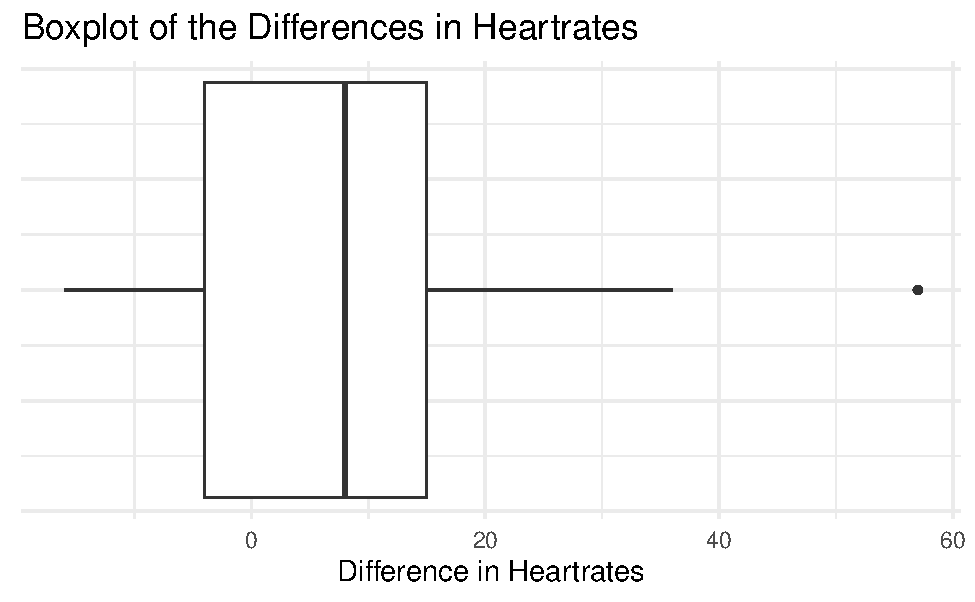
\includegraphics[width=0.6\linewidth]{14-UR-module11_review_files/figure-latex/unnamed-chunk-2-1} \end{center}

\begin{enumerate}
\def\labelenumi{\arabic{enumi}.}
\tightlist
\item
  What is the study design (observational or randomized experiment)?
\end{enumerate}

\vspace{0.5in}

\begin{enumerate}
\def\labelenumi{\arabic{enumi}.}
\setcounter{enumi}{1}
\tightlist
\item
  Is this paired study or two independent samples?
\end{enumerate}

\vspace{0.2in}

\begin{enumerate}
\def\labelenumi{\arabic{enumi}.}
\setcounter{enumi}{2}
\tightlist
\item
  Circle one answer for each bracket to complete the description of each variable listed:
\end{enumerate}

\begin{itemize}
\item
  Type of exercise (jumping jacks or bicycle kicks) is the (\emph{explanatory/response}) variable and it is (\emph{categorical/quantitative}).
\item
  Heart rate is the (\emph{explanatory/response}) variable and it is (\emph{categorical/quantitative}).
\end{itemize}

\begin{enumerate}
\def\labelenumi{\arabic{enumi}.}
\setcounter{enumi}{3}
\tightlist
\item
  What is the scope of inference for this study?
\end{enumerate}

\vspace{0.5in}

\begin{enumerate}
\def\labelenumi{\arabic{enumi}.}
\setcounter{enumi}{4}
\tightlist
\item
  Write the parameter of interest for this study.
\end{enumerate}

\vspace{0.8in}

\begin{enumerate}
\def\labelenumi{\arabic{enumi}.}
\setcounter{enumi}{5}
\tightlist
\item
  Write the null hypothesis in notation.
\end{enumerate}

\vspace{0.5in}

\begin{enumerate}
\def\labelenumi{\arabic{enumi}.}
\setcounter{enumi}{6}
\tightlist
\item
  Write the alternative hypothesis in words.
\end{enumerate}

\vspace{0.8in}

We will start with simulation methods.

\begin{enumerate}
\def\labelenumi{\arabic{enumi}.}
\setcounter{enumi}{7}
\tightlist
\item
  Calculate the difference \(\mu_0 - \bar{x}_d\). Will we need to shift the data up or down?
  \vspace{0.5in}
\end{enumerate}

\begin{Shaded}
\begin{Highlighting}[]
\FunctionTok{set.seed}\NormalTok{(}\DecValTok{216}\NormalTok{)}
\FunctionTok{paired\_test}\NormalTok{(}\AttributeTok{data =}\NormalTok{ heartrate}\SpecialCharTok{$}\NormalTok{Diff,   }\CommentTok{\#Vector of differences or data set with column for each group}
            \AttributeTok{shift =} \SpecialCharTok{{-}}\FloatTok{6.429}\NormalTok{,   }\CommentTok{\#Shift needed for bootstrap hypothesis test}
            \AttributeTok{as\_extreme\_as =} \FloatTok{6.429}\NormalTok{,  }\CommentTok{\#Observed statistic}
            \AttributeTok{direction =} \StringTok{"two{-}sided"}\NormalTok{,  }\CommentTok{\#Direction of alternative}
            \AttributeTok{number\_repetitions =} \DecValTok{10000}\NormalTok{,  }\CommentTok{\#Number of simulated samples for null distribution}
            \AttributeTok{which\_first =} \DecValTok{1}\NormalTok{)  }\CommentTok{\#Not needed when using calculated differences}
\end{Highlighting}
\end{Shaded}

\begin{center}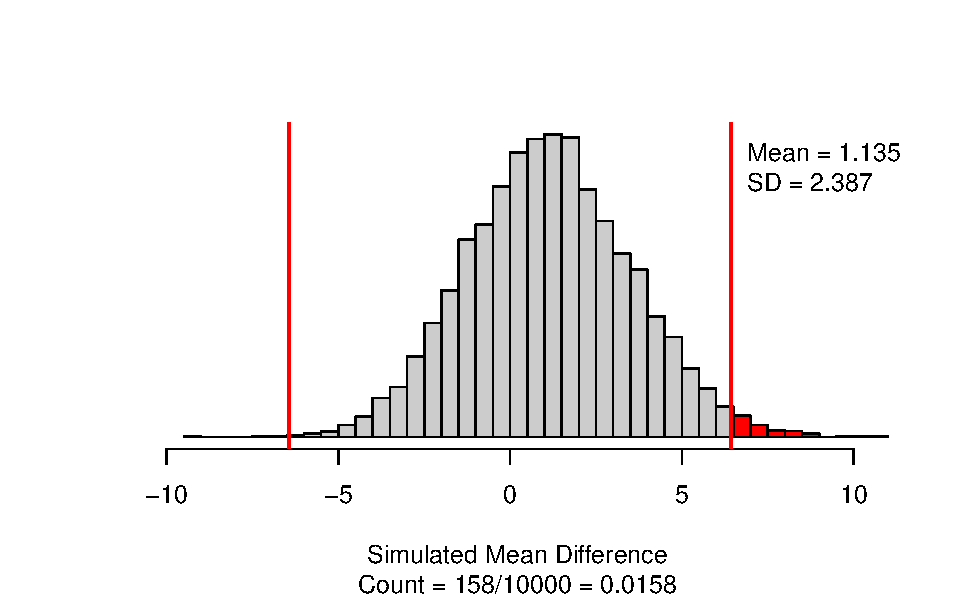
\includegraphics[width=0.7\linewidth]{14-UR-module11_review_files/figure-latex/unnamed-chunk-3-1} \end{center}

\begin{enumerate}
\def\labelenumi{\arabic{enumi}.}
\setcounter{enumi}{8}
\tightlist
\item
  Based on the p-value for this study, which of the following are true?
\end{enumerate}

\vspace{0.3mm}

\begin{itemize}
\tightlist
\item
  There is very strong evidence that there is a true difference in heart rates for students who did jumping jacks and bicycle kicks (jumping jacks -- bicycle kicks), on average.
\end{itemize}

\vspace{0.5in}

\begin{itemize}
\tightlist
\item
  If there is no true mean difference in heart rates for students who did jumping jacks and bicycle kicks, in 1 out of 1000 simulated samples, we would observe a sample mean difference in heart rates of 6.429 bpm or more extreme.
\end{itemize}

\vspace{0.5in}

\begin{itemize}
\tightlist
\item
  The 95\% confidence interval would be entirely positive.
\end{itemize}

\vspace{0.5in}

\begin{itemize}
\tightlist
\item
  There could be a potential Type I error.
\end{itemize}

\vspace{0.5in}

\begin{itemize}
\tightlist
\item
  We would conclude that there is evidence of a difference in heart rates between exercises, on average, when in fact there is not.
\end{itemize}

\vspace{0.5in}

Bootstrap CI simulation to create a 95\% confidence interval

\begin{Shaded}
\begin{Highlighting}[]
\FunctionTok{paired\_bootstrap\_CI}\NormalTok{(}\AttributeTok{data =}\NormalTok{ heartrate}\SpecialCharTok{$}\NormalTok{Diff, }\CommentTok{\#Enter vector of differences}
                    \AttributeTok{number\_repetitions =} \DecValTok{10000}\NormalTok{, }\CommentTok{\#Number of bootstrap samples for CI}
                    \AttributeTok{confidence\_level =} \FloatTok{0.95}\NormalTok{,  }\CommentTok{\#Confidence level in decimal form}
                    \AttributeTok{which\_first =} \DecValTok{1}\NormalTok{)  }\CommentTok{\#Not needed when entering vector of differences}
\end{Highlighting}
\end{Shaded}

\begin{center}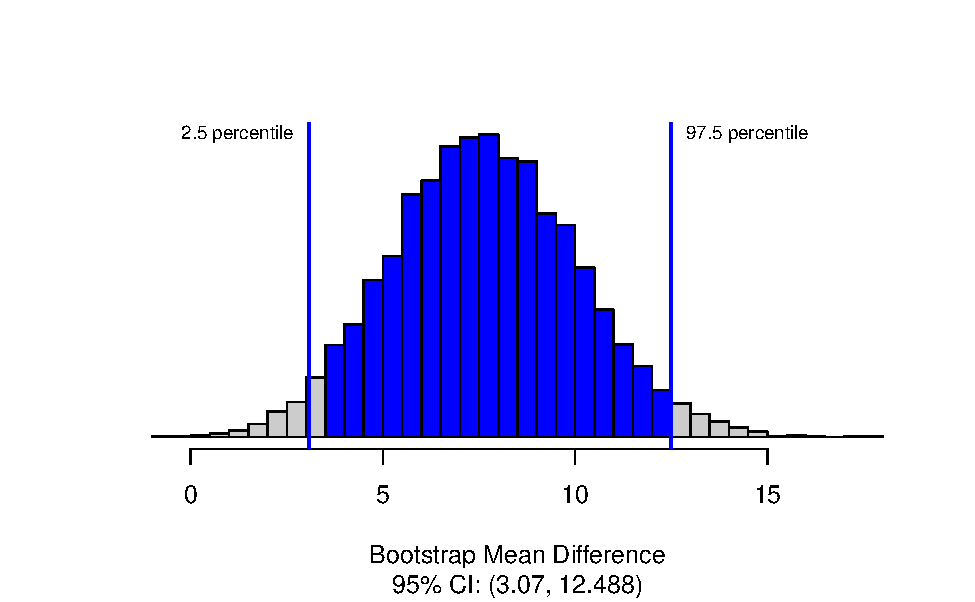
\includegraphics[width=0.7\linewidth]{14-UR-module11_review_files/figure-latex/unnamed-chunk-4-1} \end{center}

\begin{enumerate}
\def\labelenumi{\arabic{enumi}.}
\setcounter{enumi}{9}
\tightlist
\item
  Interpret the 95\% confidence interval in context of the study.
\end{enumerate}

\vspace{0.8in}

\begin{enumerate}
\def\labelenumi{\arabic{enumi}.}
\setcounter{enumi}{10}
\tightlist
\item
  Interpret the confidence level in context of the study. What does confidence mean?
\end{enumerate}

\vspace{0.8in}

Next we will use theory-based methods.

The sampling distribution for \(\bar{x}\) based on a sample of size \(n\) from a population with a true mean \(\mu\) and true standard deviation \(\sigma\) can be modeled using a normal distribution when certain conditions are met.

Conditions for the sampling distribution of \(\bar{x}\) to follow an approximate normal distribution:

\begin{itemize}
\item
  \textbf{Independence}: The sample's observations are independent
\item
  \textbf{Normality}: The data should be approximately normal or the sample size should be large.

  \begin{itemize}
  \item
    \(n < 30\): If the sample size \(n\) is less than 30 and there are no clear outliers in the distribution of differences, then we typically assume the data come from a nearly normal distribution to satisfy the condition.
  \item
    \(30 \le n < 100\): If the sample size \(n\) is between 30 and 100 and there are no particularly extreme outliers in the differences of differences, then we typically assume the sampling distribution of \(\bar{x}\) is nearly normal to satisfy the condition
  \item
    \(n \ge 100\): If the sample size is greater than 100 then we typically assume the sampling distribution of \(\bar{x}\) is nearly normal to satisfy the condition, even if the underlying distribution of individual observations is not.
  \end{itemize}
\end{itemize}

\begin{enumerate}
\def\labelenumi{\arabic{enumi}.}
\setcounter{enumi}{11}
\tightlist
\item
  Are the conditions met to model the data with theory-based methods?
\end{enumerate}

\vspace{0.8in}

To find the standardized statistic for the paired differences we will use the following formula:

\[T = \frac{\bar{x}_d - \text{null value}}{SE(\bar{x}_d)},\]

where the standard error of the sample mean difference is:

\[SE(\bar{x}_d)=\frac{s_d}{\sqrt{n}}.\]
13. Calculate the standard error of the mean difference.

\vspace{0.8in}

\begin{enumerate}
\def\labelenumi{\arabic{enumi}.}
\setcounter{enumi}{13}
\tightlist
\item
  Calculate the standardized mean difference.
\end{enumerate}

\vspace{0.8in}

\begin{enumerate}
\def\labelenumi{\arabic{enumi}.}
\setcounter{enumi}{14}
\tightlist
\item
  Interpret the standardized statistic in context of the problem.
\end{enumerate}

\vspace{0.8in}

\begin{Shaded}
\begin{Highlighting}[]
\DecValTok{2}\SpecialCharTok{*}\FunctionTok{pt}\NormalTok{(}\FloatTok{2.957}\NormalTok{, }\AttributeTok{df=}\DecValTok{41}\NormalTok{, }\AttributeTok{lower.tail=}\ConstantTok{FALSE}\NormalTok{)}
\CommentTok{\#\textgreater{} [1] 0.005134632}
\end{Highlighting}
\end{Shaded}

\newpage

\begin{figure}

{\centering 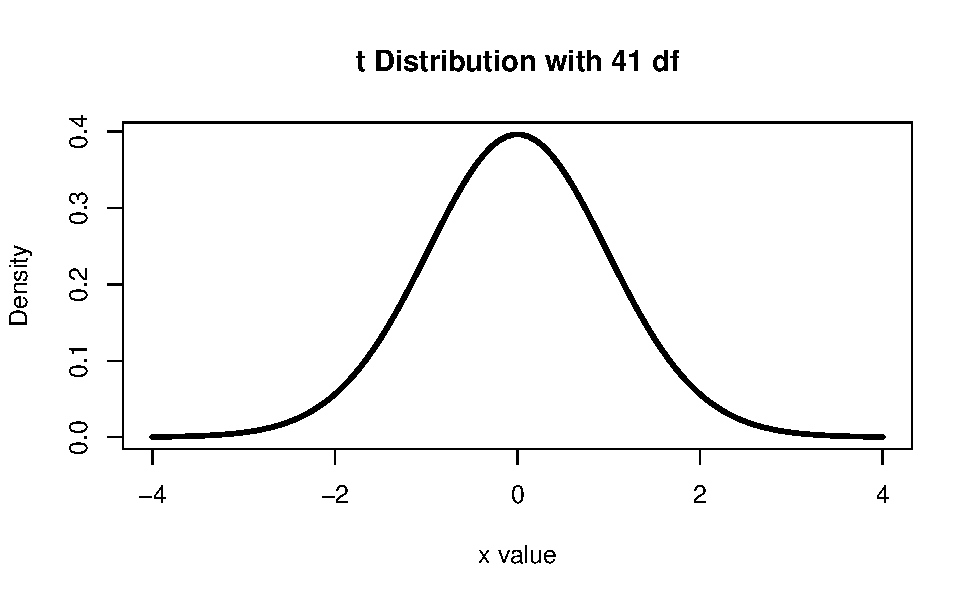
\includegraphics[width=0.7\linewidth]{14-UR-module11_review_files/figure-latex/pvalue-1} 

}

\caption{t-distribution with 41 degrees of freedom}\label{fig:pvalue}
\end{figure}

To calculate the 95\% theory-based confidence interval for the paired mean difference, use the following formula:

\[\bar{x}_d\pm t^* SE(\bar{x}_d).\]

We will need to find the \(t^*\) multiplier using the function \texttt{qt()}. For a 95\% confidence level, we are finding the \(t^*\) value at the 97.5th percentile with \texttt{df} = \(n_d - 1 = 42 - 1 = 41\).

\newpage

\begin{Shaded}
\begin{Highlighting}[]
\FunctionTok{qt}\NormalTok{(}\FloatTok{0.975}\NormalTok{, }\AttributeTok{df =} \DecValTok{41}\NormalTok{, }\AttributeTok{lower.tail=}\ConstantTok{TRUE}\NormalTok{)}
\CommentTok{\#\textgreater{} [1] 2.019541}
\end{Highlighting}
\end{Shaded}

\begin{figure}

{\centering 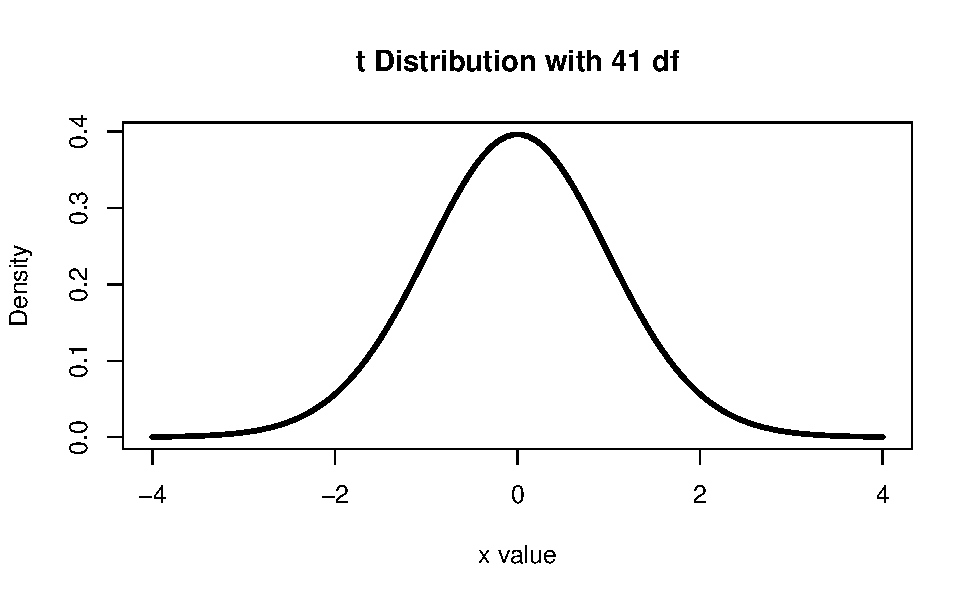
\includegraphics[width=0.7\linewidth]{14-UR-module11_review_files/figure-latex/tstar-1} 

}

\caption{t-distribution with 41 degrees of freedom}\label{fig:tstar}
\end{figure}

\begin{enumerate}
\def\labelenumi{\arabic{enumi}.}
\setcounter{enumi}{15}
\tightlist
\item
  Calculate the 95\% confidence interval.
\end{enumerate}

\vspace{0.8in}

\begin{enumerate}
\def\labelenumi{\arabic{enumi}.}
\setcounter{enumi}{16}
\tightlist
\item
  Write a conclusion to the research question.
\end{enumerate}

\section{Module 12 Review - Independent Samples}\label{module-12-review---independent-samples}

The ``social brain hypothesis,'' or the ``social intelligence hypothesis,'' suggests that living in socially cohesive groups with differentiated relationships requires a higher cognitive load, in turn resulting in higher brain volume. There is evidence this hypothesis holds for primates and some other mammal groups, but it hasn't been explored in birds, as most birds typically have temporary social groupings that lack clear relationships. However, woodpeckers have a wide range of clearly differing social relationships while also having the benefit of being physiologically and environmentally similar across species. Researchers want to know if the ``social brain hypothesis'' holds true for woodpeckers: is the average brain volume (in mm\^{}3) smaller for woodpeckers that tend to be solitary compared to woodpeckers that tend to live in pairs or groups? For the purpose of this study, ``solitary'' birds are classified as those that only pair-bond to breed, and otherwise are solitary for more than half a year each year. ``Group-living'' birds are those that spend more than half the year in communal groups or flocks. Researchers examined 61 species of woodpeckers. Use solitary - group living as the order of subtraction

The summary of the data and boxplots are given below:

\begin{Shaded}
\begin{Highlighting}[]
\NormalTok{woodpeckers }\OtherTok{\textless{}{-}} \FunctionTok{read.csv}\NormalTok{(}\StringTok{"data/woodpeckers.csv"}\NormalTok{)}
\CommentTok{\# Summary statistics}
\NormalTok{woodpeckers }\SpecialCharTok{\%\textgreater{}\%} 
    \FunctionTok{reframe}\NormalTok{(}\FunctionTok{favstats}\NormalTok{(Volume}\SpecialCharTok{\textasciitilde{}}\NormalTok{SocialCategory))}
\CommentTok{\#\textgreater{}   SocialCategory min      Q1 median     Q3  max     mean       sd  n missing}
\CommentTok{\#\textgreater{} 1   group\_living 292 1623.75 2731.5 4562.5 7856 3179.900 2062.236 20       0}
\CommentTok{\#\textgreater{} 2       solitary 600 1450.00 2106.0 3060.0 7700 2483.927 1539.478 41       0}
\end{Highlighting}
\end{Shaded}

\begin{Shaded}
\begin{Highlighting}[]
\CommentTok{\# Side{-}by{-}side box plots}
\NormalTok{woodpeckers }\SpecialCharTok{\%\textgreater{}\%}
\FunctionTok{ggplot}\NormalTok{(}\FunctionTok{aes}\NormalTok{(}\AttributeTok{x =}\NormalTok{ SocialCategory, }\AttributeTok{y =}\NormalTok{ Volume)) }\SpecialCharTok{+}
    \FunctionTok{geom\_boxplot}\NormalTok{() }\SpecialCharTok{+} 
    \FunctionTok{labs}\NormalTok{(}\AttributeTok{title =} \StringTok{"Boxplots of Brain Volume for Woodpeckers by Social Grouping"}\NormalTok{,}
         \AttributeTok{x =} \StringTok{"Social Grouping"}\NormalTok{, }
         \AttributeTok{y =} \StringTok{"Brain Volume (mm\^{}3"}\NormalTok{) }
  
\end{Highlighting}
\end{Shaded}

\begin{center}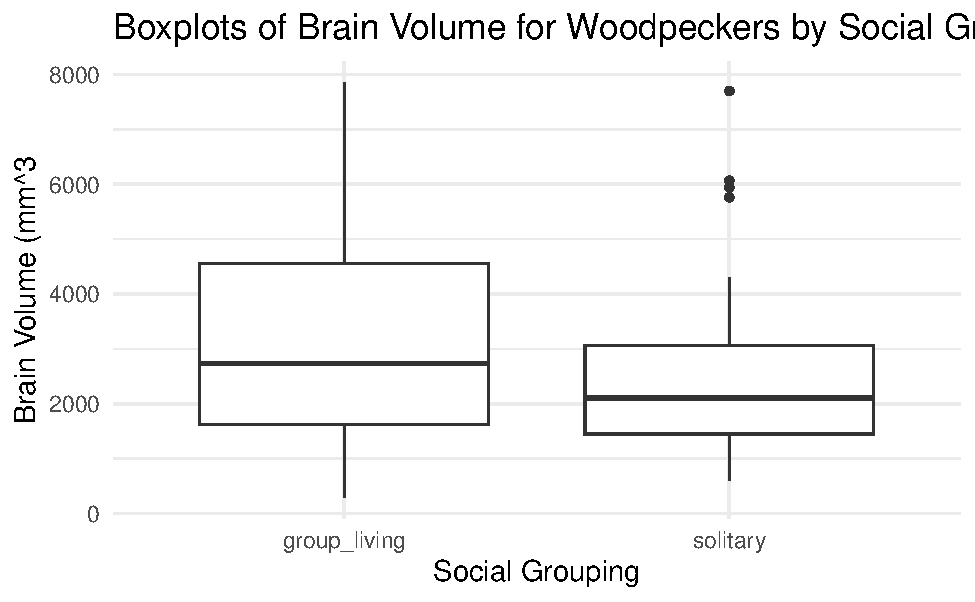
\includegraphics[width=0.6\linewidth]{14-UR-module12_review_files/figure-latex/unnamed-chunk-2-1} \end{center}

\begin{enumerate}
\def\labelenumi{\arabic{enumi}.}
\tightlist
\item
  Write out the parameter of interest in context of the problem. Use proper notation.
\end{enumerate}

\vspace{0.5in}

\begin{enumerate}
\def\labelenumi{\arabic{enumi}.}
\setcounter{enumi}{1}
\tightlist
\item
  Write the null hypothesis in notation.
\end{enumerate}

\vspace{0.5in}

\begin{enumerate}
\def\labelenumi{\arabic{enumi}.}
\setcounter{enumi}{2}
\tightlist
\item
  Write the alternative hypothesis in words.
\end{enumerate}

\vspace{0.5in}

\begin{enumerate}
\def\labelenumi{\arabic{enumi}.}
\setcounter{enumi}{3}
\tightlist
\item
  Calculate the summary statistic. Use proper notation.
\end{enumerate}

\vspace{0.5in}

\textbf{Simulation Methods}

\textbf{Hypothesis Testing}

In the two\_mean\_test function, enter the response\textasciitilde explanatory variable names in for the formula (response\textasciitilde explanatory) and the name of the data set (woodpeckers) for data. Since the order of subtraction is \texttt{solitary} - \texttt{group\_living} enter \texttt{solitary} for first\_in\_subtraction. Enter the summary statistic in for as\_extreme\_as and choose the direction to match the alternative hypothesis.

\begin{Shaded}
\begin{Highlighting}[]
\FunctionTok{set.seed}\NormalTok{(}\DecValTok{216}\NormalTok{)}
\FunctionTok{two\_mean\_test}\NormalTok{(Volume}\SpecialCharTok{\textasciitilde{}}\NormalTok{SocialCategory, }\AttributeTok{data =}\NormalTok{ woodpeckers,  }\CommentTok{\#Variables and data}
                    \AttributeTok{first\_in\_subtraction =} \StringTok{"solitary"}\NormalTok{, }\CommentTok{\#First value in order of subtraction}
                    \AttributeTok{number\_repetitions =} \DecValTok{10000}\NormalTok{,  }\CommentTok{\#Number of simulations}
                    \AttributeTok{as\_extreme\_as =} \SpecialCharTok{{-}}\FloatTok{695.973}\NormalTok{, }\CommentTok{\#Observed statistic}
                    \AttributeTok{direction =} \StringTok{"less"}\NormalTok{)  }\CommentTok{\#Direction of alternative: "greater", "less", or "two{-}sided"}
\end{Highlighting}
\end{Shaded}

\begin{center}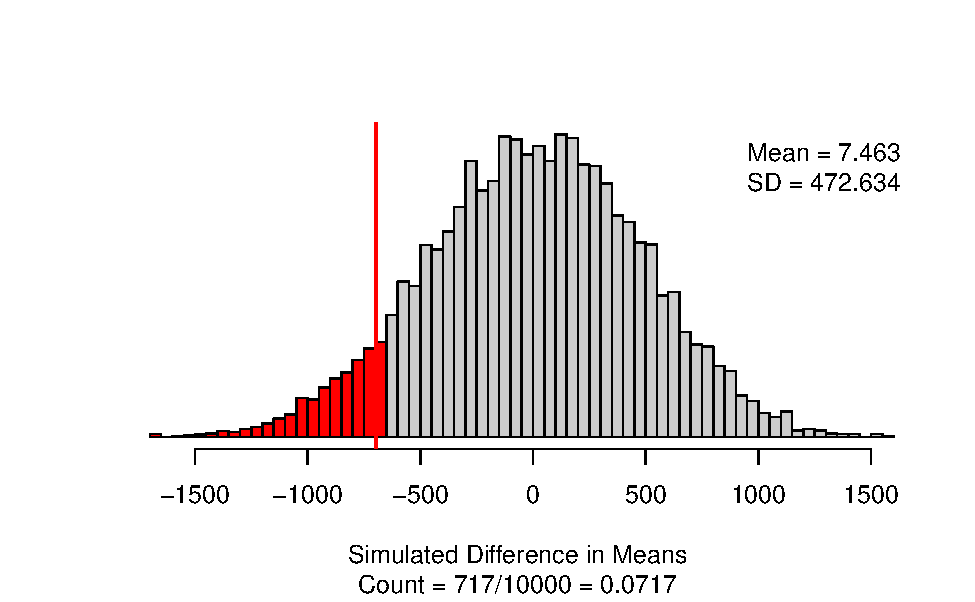
\includegraphics[width=0.7\linewidth]{14-UR-module12_review_files/figure-latex/unnamed-chunk-3-1} \end{center}

\begin{enumerate}
\def\labelenumi{\arabic{enumi}.}
\setcounter{enumi}{4}
\tightlist
\item
  Based on the p-value for this study, explain why each of the following are false.
\end{enumerate}

\begin{enumerate}
\def\labelenumi{\Alph{enumi}.}
\tightlist
\item
  There is strong evidence that there is a true mean difference in brain volume for species of woodpeckers that live solo and those that live in groups (solitary - group).
\end{enumerate}

\vspace{0.5in}

\begin{enumerate}
\def\labelenumi{\Alph{enumi}.}
\setcounter{enumi}{1}
\tightlist
\item
  If the difference in true mean brain volume for species of woodpeckers that live solo and that live in groups is less than zero, in 58 out of 1000 samples, we would observe a sample difference in mean brain volume of -695.973 \(mm^3\) or less.
\end{enumerate}

\vspace{0.5in}

\begin{enumerate}
\def\labelenumi{\Alph{enumi}.}
\setcounter{enumi}{2}
\tightlist
\item
  The 99\% confidence interval would not include the value of zero.
\end{enumerate}

\vspace{0.5in}

\begin{enumerate}
\def\labelenumi{\Alph{enumi}.}
\setcounter{enumi}{3}
\tightlist
\item
  We could conclude that the brain volume for species of woodpeckers that live solo is less than for those that live in groups when in fact there is no difference in brain volume for species of woodpeckers that live solo and that live in groups.
\end{enumerate}

\vspace{0.5in}

\newpage

\textbf{Bootstrap Confidence Interval}
To find the 99\% confidence interval for the true difference in mean brain volume for species of woodpeckers that live in groups and species of woodpeckers that live solo use the two\_mean\_bootstrap\_CI. The inputs are similar as to what we used in the two\_mean\_test.

\begin{Shaded}
\begin{Highlighting}[]
\FunctionTok{set.seed}\NormalTok{(}\DecValTok{216}\NormalTok{)}
\FunctionTok{two\_mean\_bootstrap\_CI}\NormalTok{(Volume}\SpecialCharTok{\textasciitilde{}}\NormalTok{SocialCategory, }\AttributeTok{data =}\NormalTok{ woodpeckers,  }\CommentTok{\#Variables and data}
                      \AttributeTok{first\_in\_subtraction =} \StringTok{"solitary"}\NormalTok{, }\CommentTok{\#First value in order of subtraction}
                      \AttributeTok{number\_repetitions =} \DecValTok{10000}\NormalTok{,  }\CommentTok{\#Number of simulations}
                      \AttributeTok{confidence\_level =} \FloatTok{0.99}\NormalTok{)}
\end{Highlighting}
\end{Shaded}

\begin{center}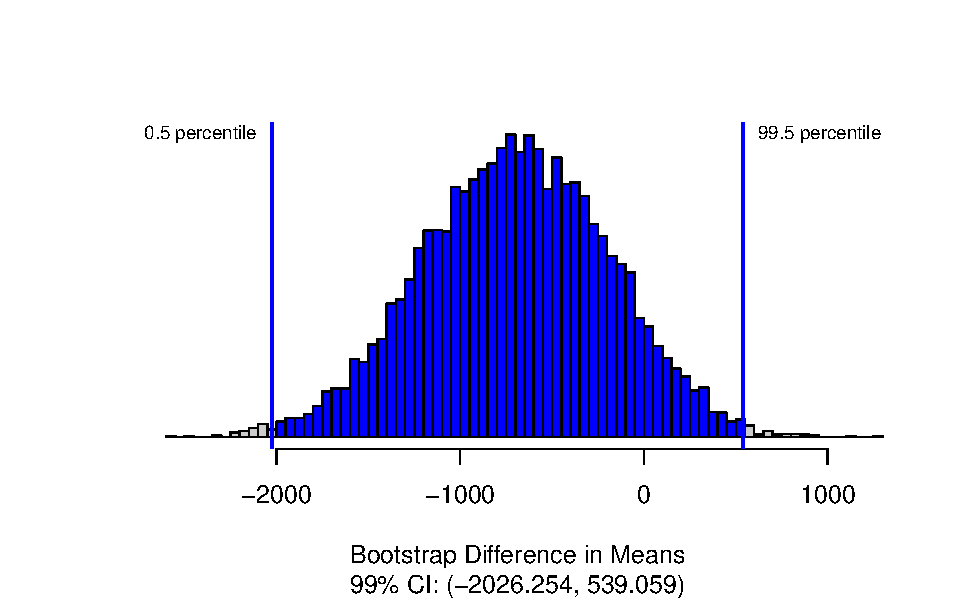
\includegraphics[width=0.7\linewidth]{14-UR-module12_review_files/figure-latex/unnamed-chunk-4-1} \end{center}

\begin{enumerate}
\def\labelenumi{\arabic{enumi}.}
\setcounter{enumi}{5}
\tightlist
\item
  Interpret the confidence interval in context of the problem.
\end{enumerate}

\vspace{0.5in}

\begin{enumerate}
\def\labelenumi{\arabic{enumi}.}
\setcounter{enumi}{6}
\tightlist
\item
  Write a conclusion to the research question.
\end{enumerate}

\vspace{0.5in}

\newpage

\textbf{Hypothesis testing using theory-based methods}

Standardized Statistic:

~~~~\(T = \frac{\bar{x}_1 - \bar{x}_2-\mbox{null value}}{SE(\bar{x}_1 - \bar{x}_2)}\)

~~~~\(SE(\bar{x}_1 - \bar{x}_2)=\sqrt{\frac{s_1^2}{n_1}+\frac{s_2^2}{n_2}}\)

\begin{enumerate}
\def\labelenumi{\arabic{enumi}.}
\setcounter{enumi}{7}
\tightlist
\item
  Calculate the standard error of the difference in means.
\end{enumerate}

\vspace{0.5in}

\begin{enumerate}
\def\labelenumi{\arabic{enumi}.}
\setcounter{enumi}{8}
\tightlist
\item
  Calculate the standardized difference in sample mean.
\end{enumerate}

\vspace{0.5in}

Enter the t score into the pt function using a df = minimum(n - 1) = 20 - 1 = 19, and lower.tail = FALSE.

\begin{Shaded}
\begin{Highlighting}[]
\FunctionTok{pt}\NormalTok{(}\SpecialCharTok{{-}}\FloatTok{1.338}\NormalTok{, }\AttributeTok{df=}\DecValTok{19}\NormalTok{, }\AttributeTok{lower.tail=}\ConstantTok{TRUE}\NormalTok{)}
\CommentTok{\#\textgreater{} [1] 0.09834555}
\end{Highlighting}
\end{Shaded}

\begin{enumerate}
\def\labelenumi{\arabic{enumi}.}
\setcounter{enumi}{9}
\tightlist
\item
  Why do we use lower.tail=TRUE to find the p-value?
  \vspace{0.5in}
\end{enumerate}

\textbf{Confidence interval using theory-based methods}

To calculate the 99\% confidence interval we use the formula:

\(\bar{x}_1- \bar{x}_2\pm t^* \times SE(\bar{x}_1- \bar{x}_2)\) we will need to find the \(t^*\) multiplier using the function qt.

For a 95\% confidence interval we are finding the \(t^*\) value at the 99.5th percentile with df = minimum(n - 1) = 20 - 1 = 19.

\begin{Shaded}
\begin{Highlighting}[]
\FunctionTok{qt}\NormalTok{(}\FloatTok{0.995}\NormalTok{, }\AttributeTok{df =} \DecValTok{19}\NormalTok{, }\AttributeTok{lower.tail=}\ConstantTok{TRUE}\NormalTok{)}
\CommentTok{\#\textgreater{} [1] 2.860935}
\end{Highlighting}
\end{Shaded}

\begin{enumerate}
\def\labelenumi{\arabic{enumi}.}
\setcounter{enumi}{10}
\tightlist
\item
  Calculate the 99\% confidence interval.
\end{enumerate}

\vspace{0.5in}

\begin{enumerate}
\def\labelenumi{\arabic{enumi}.}
\setcounter{enumi}{11}
\tightlist
\item
  Why do the simulation and theory based methods not give the same results?
\end{enumerate}

\vspace{0.5in}

\section{Module 13 Review - Regression}\label{module-13-review---regression}

Spotify created a list of the top songs around the world for the past 10 years and several different audio features of those songs. Among the variables measured on these songs, we will look at the relationship between Valance and Danceability. Valance measures the positive mood of a song; the higher the point value the more positive the mood of the song. Danceability measures how easy it is to dance to a song; the higher the point value the easier it is to dance to the song. Is there evidence that songs with a higher valance value are more danceable, on average?

\begin{Shaded}
\begin{Highlighting}[]
\NormalTok{songs }\OtherTok{\textless{}{-}} \FunctionTok{read.csv}\NormalTok{(}\StringTok{"data/top10s.csv"}\NormalTok{) }\CommentTok{\#Reads in data set}
\NormalTok{songs }\SpecialCharTok{\%\textgreater{}\%} \CommentTok{\#Data set pipes into...}
\FunctionTok{ggplot}\NormalTok{(}\FunctionTok{aes}\NormalTok{(}\AttributeTok{x =}\NormalTok{ Valance, }\AttributeTok{y =}\NormalTok{ Danceability))}\SpecialCharTok{+}  \CommentTok{\#Specify variables}
  \FunctionTok{geom\_point}\NormalTok{() }\SpecialCharTok{+}  \CommentTok{\#Add scatterplot of points}
  \FunctionTok{labs}\NormalTok{(}\AttributeTok{x =} \StringTok{"valance"}\NormalTok{,  }\CommentTok{\#Label x{-}axis}
       \AttributeTok{y =} \StringTok{"danceability"}\NormalTok{,  }\CommentTok{\#Label y{-}axis}
       \AttributeTok{title =} \StringTok{"Scatterplot of Valance vs. Danceability for Top songs"}\NormalTok{) }\SpecialCharTok{+} \CommentTok{\#Be sure to title your plot}
  \FunctionTok{theme\_bw}\NormalTok{()  }\CommentTok{\#Add regression line}
\end{Highlighting}
\end{Shaded}

\begin{center}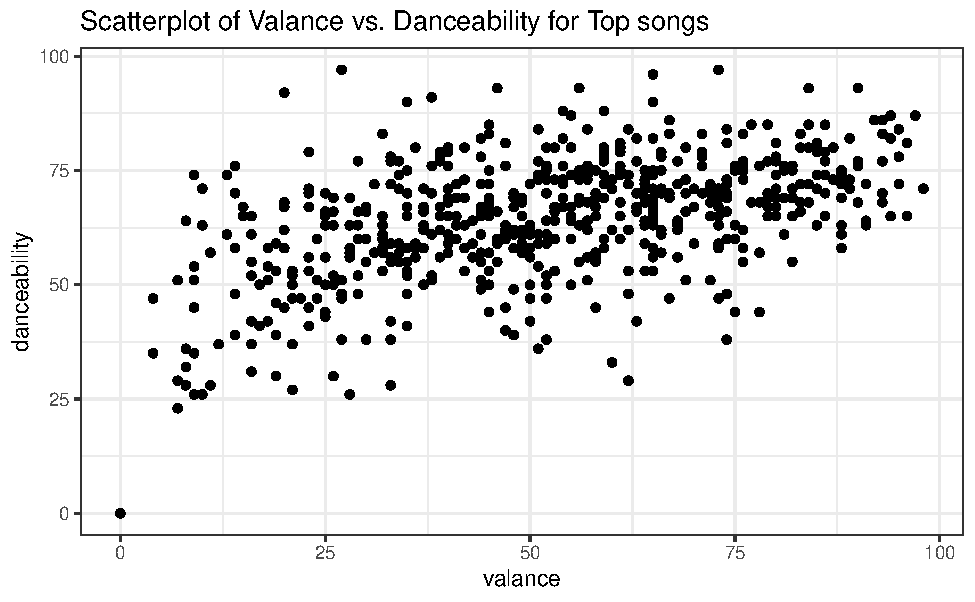
\includegraphics[width=0.7\linewidth]{14-UR-module13_review_files/figure-latex/unnamed-chunk-1-1} \end{center}

\begin{enumerate}
\def\labelenumi{\arabic{enumi}.}
\tightlist
\item
  Identify the explanatory variable and the response variable.
\end{enumerate}

\newpage

The linear model output is given below with the correlation coefficient.

\begin{Shaded}
\begin{Highlighting}[]
\CommentTok{\# Fit linear model: y \textasciitilde{} x}
\NormalTok{songsLM }\OtherTok{\textless{}{-}} \FunctionTok{lm}\NormalTok{(Danceability}\SpecialCharTok{\textasciitilde{}}\NormalTok{Valance, }\AttributeTok{data=}\NormalTok{songs)}
\FunctionTok{round}\NormalTok{(}\FunctionTok{summary}\NormalTok{(songsLM)}\SpecialCharTok{$}\NormalTok{coefficients, }\DecValTok{5}\NormalTok{) }\CommentTok{\# Display coefficient summary}
\end{Highlighting}
\end{Shaded}

\begin{verbatim}
#>             Estimate Std. Error  t value Pr(>|t|)
#> (Intercept) 48.80920    1.19239 40.93393        0
#> Valance      0.29814    0.02097 14.21805        0
\end{verbatim}

\begin{Shaded}
\begin{Highlighting}[]
\FunctionTok{cor}\NormalTok{(songs}\SpecialCharTok{$}\NormalTok{Danceability, songs}\SpecialCharTok{$}\NormalTok{Valance)}
\end{Highlighting}
\end{Shaded}

\begin{verbatim}
#> [1] 0.5016962
\end{verbatim}

\begin{enumerate}
\def\labelenumi{\arabic{enumi}.}
\setcounter{enumi}{1}
\tightlist
\item
  Write the least squares equation of the regression line in context of the problem.
\end{enumerate}

\vspace{0.5in}

\begin{enumerate}
\def\labelenumi{\arabic{enumi}.}
\setcounter{enumi}{2}
\tightlist
\item
  Interpret the slope in context of the problem.
\end{enumerate}

\vspace{0.5in}

\begin{enumerate}
\def\labelenumi{\arabic{enumi}.}
\setcounter{enumi}{3}
\tightlist
\item
  Write the null hypothesis, in words, in context of the problem.
\end{enumerate}

\vspace{1in}

\begin{enumerate}
\def\labelenumi{\arabic{enumi}.}
\setcounter{enumi}{4}
\tightlist
\item
  Write the alternative hypothesis, in notation, to test slope, in context of the problem.
\end{enumerate}

\vspace{0.5in}

\emph{Simulation Methods}

The following code creates the null distribution for this study.

\begin{center}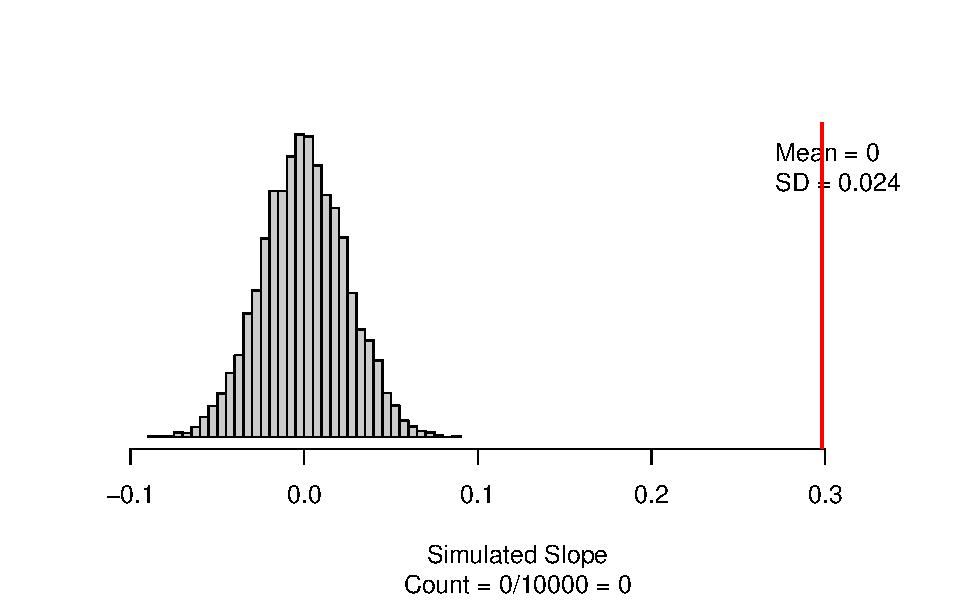
\includegraphics[width=0.7\linewidth]{14-UR-module13_review_files/figure-latex/unnamed-chunk-3-1} \end{center}

\begin{enumerate}
\def\labelenumi{\arabic{enumi}.}
\setcounter{enumi}{5}
\tightlist
\item
  Report the value of the p-value. Interpret this value in context of the problem.
\end{enumerate}

\vspace{1in}

\begin{enumerate}
\def\labelenumi{\arabic{enumi}.}
\setcounter{enumi}{6}
\tightlist
\item
  Based on the p-value, write a conclusion in context of the problem.
\end{enumerate}

\vspace{1in}

Now let's estimate the true regression slope for the relationship between valance and danceability of songs.

\begin{center}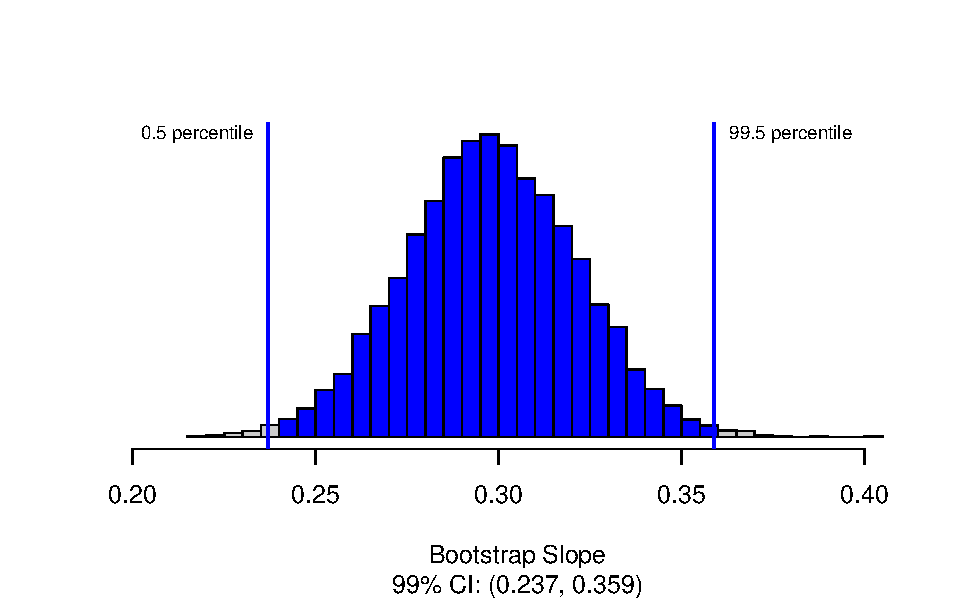
\includegraphics[width=0.7\linewidth]{14-UR-module13_review_files/figure-latex/unnamed-chunk-4-1} \end{center}

\begin{enumerate}
\def\labelenumi{\arabic{enumi}.}
\setcounter{enumi}{7}
\tightlist
\item
  Interpret the 99\% confidence interval in context of the problem.
\end{enumerate}

\vspace{1in}

Now let's test correlation.

\begin{enumerate}
\def\labelenumi{\arabic{enumi}.}
\setcounter{enumi}{8}
\tightlist
\item
  How will the null and alternative hypotheses change?
\end{enumerate}

\vspace{0.5in}

\begin{center}\includegraphics[width=0.7\linewidth]{14-UR-module13_review_files/figure-latex/unnamed-chunk-5-1} \end{center}

\begin{center}\includegraphics[width=0.7\linewidth]{14-UR-module13_review_files/figure-latex/unnamed-chunk-6-1} \end{center}

\begin{enumerate}
\def\labelenumi{\arabic{enumi}.}
\setcounter{enumi}{9}
\tightlist
\item
  Interpret the 99\% confidence interval for the true correlation between valance and danceability.
\end{enumerate}

\newpage

\emph{Theory-based Methods}

When performing inference on a least squares line, the follow conditions are generally required

\begin{itemize}
\item
  Linearity: the data should follow a linear trend
\item
  Nearly normal residuals: residuals must be nearly normal
\item
  Constant variability: the variability of points around the least squares line remains roughly constant
\item
  Independent observations: individual data points must be independent
\end{itemize}

The scatterplot and the residual plots will be used to assess the conditions for approximating the data with the \(t\)-distribution.

\begin{center}\includegraphics[width=0.7\linewidth]{14-UR-module13_review_files/figure-latex/unnamed-chunk-7-1} \end{center}

\begin{enumerate}
\def\labelenumi{\arabic{enumi}.}
\setcounter{enumi}{10}
\tightlist
\item
  Are the conditions met to use the \(t\)-distribution to approximate the sampling distribution of our test statistic?
\end{enumerate}

\newpage

To find the value of the test statistic to test the slope we will use,

\[
T = \frac{b_1- \text{null value}}{SE(b_1)}
\]

We will use the linear model output above to get the estimate for slope and standard error.

\begin{enumerate}
\def\labelenumi{\arabic{enumi}.}
\setcounter{enumi}{11}
\tightlist
\item
  Calculate the standardized slope.
\end{enumerate}

\vspace{1in}

\begin{enumerate}
\def\labelenumi{\arabic{enumi}.}
\setcounter{enumi}{12}
\tightlist
\item
  Using the linear model output, report the p-value for the test of significance.
\end{enumerate}

\vspace{0.5in}

\begin{enumerate}
\def\labelenumi{\arabic{enumi}.}
\setcounter{enumi}{13}
\tightlist
\item
  Based on the p-value, how much evidence is there against the null hypothesis?
\end{enumerate}

\vspace{0.5in}

Recall that a confidence interval is calculated by adding and subtracting the margin of error to the point estimate.\\
\[\mbox{point estimate}\pm t^* \times SE(estimate)\]
\[b_1 \pm t^* \times SE(b_1)\]

The \(t^*\) multiplier comes from the \(t\)-distribution with \(n-2\) df. Recall for a 99\% confidence interval, use the 99.5\% percentile (99\% of the distribution is in the middle, leaving 0.5\% in each tail). The sample size is 603 so the df is 601.

\begin{Shaded}
\begin{Highlighting}[]
\FunctionTok{qt}\NormalTok{(}\FloatTok{0.995}\NormalTok{, }\DecValTok{601}\NormalTok{) }\CommentTok{\#95\% t* multiplier }
\end{Highlighting}
\end{Shaded}

\begin{verbatim}
#> [1] 2.584034
\end{verbatim}

\begin{enumerate}
\def\labelenumi{\arabic{enumi}.}
\setcounter{enumi}{14}
\tightlist
\item
  Calculate the 99\% confidence interval for the true slope.
  \vspace{1in}
\end{enumerate}

\section{Unit 3 Review}\label{unit-3-review-1}

\subsection{Key Topics Exam 3}\label{key-topics-exam-3}

Descriptive statistics and study design:

\begin{enumerate}
\def\labelenumi{\arabic{enumi}.}
\item
  Identify the observational units.
\item
  Identify the types of variables (categorical or quantitative).
\item
  Identify the explanatory variable (if present) and the response variable (roles of variables).
\item
  Identify the appropriate type of graph and summary measure.
\item
  Identify the study design (observational study or randomized experiment).
\item
  Identify the sampling method and potential types of sampling bias (non-response, response, selection).
\item
  Determine the scope of inference (causation/association and generalizability) of the study.
\item
  Calculate and interpret the mean difference from paired data.
\item
  Calculate and interpret the difference in means from independent data.
\item
  Identify the slope of the repression line from R output and interpret.
\item
  Identify the correlation from R output and describe the strength and direction.
\item
  Calculate and interpret coefficient of determination.
\end{enumerate}

Hypothesis testing:

\begin{enumerate}
\def\labelenumi{\arabic{enumi}.}
\setcounter{enumi}{12}
\item
  Identify which of the three scenarios applies to the study: paired data, independent groups, or two quantitative variables.
\item
  Write the parameter of interest in words and correct notation.
\item
  Find the value of the observed statistic (point estimate, summary statistic). Use correct notation.
\item
  State the null and alternative hypotheses in words and in correct notation.
\item
  Verify the validity condition is met to use simulation-based methods to find a p-value.
\item
  Verify the validity conditions are met to use theory-based methods to find a p-value from the theoretical distribution.
\item
  In a simulation-based hypothesis test, describe how to create one dot on a dotplot of the null distribution using cards.
\item
  Explain where the null distribution is centered and why.
\item
  Describe and illustrate how R calculates the p-value for a simulation-based test.
\item
  Describe and illustrate how R calculates the p-value for a theory-based test.
\item
  Type of theoretical distribution (t-distribution and appropriate degrees of freedom) used to model the standardized statistic in a theory-based hypothesis test.
\item
  Calculate and interpret the standard error of the statistic using the correct formula on the Golden ticket.
\item
  Calculate and interpret the appropriate standardized statistic using the correct formula on the Golden ticket.
\item
  Interpret the p-value in context of the study: it is the probability of \_\_\_\_, assuming \_\_\_\_.
\item
  Evaluate the p-value for strength of evidence against the null: how much evidence does the p-value provide against the null?
\item
  Write a conclusion about the research question based on the p-value.
\item
  Given a significance level, what decision can be made about the research question based on the p-value.
\end{enumerate}

Confidence interval:

\begin{enumerate}
\def\labelenumi{\arabic{enumi}.}
\setcounter{enumi}{29}
\item
  Describe how to simulate one bootstrapped sample using cards.
\item
  Explain where the bootstrap distribution is centered and why.
\item
  Find an appropriate percentile confidence interval using a bootstrap distribution from R output.
\item
  Verify the validity condition is met to use simulation-based methods to find the confidence interval.
\item
  Verify the validity conditions are met to use theory-based methods to calculate a confidence interval.
\item
  Describe and illustrate how the bootstrap distribution is used to find the confidence interval for a given confidence level.
\item
  Describe and illustrate how the t-distribution is used to find the multiplier for a given confidence level.
\item
  Calculate the appropriate margin of error and confidence interval using theory-based methods.
\item
  Interpret the confidence interval in context of the study.
\item
  Based on the interval, what decision can you make about the null hypothesis? Does the confidence interval agree with the results of the hypothesis test? Justify your answer.
\item
  Interpret the confidence level in context of the study. What does ``confidence'' mean?
\item
  Describe which features of the study have an effect on the width of the confidence interval and how.
\end{enumerate}

\newpage

\chapter*{References}\label{references}
\addcontentsline{toc}{chapter}{References}

\phantomsection\label{refs}
\begin{CSLReferences}{1}{0}
\bibitem[\citeproctext]{ref-pga}
{``Average Driving Distance and Fairway Accuracy.''} 2008. \href{https://www.pga.com/\%20and\%20https://www.lpga.com/}{https://www.pga.com/ and https://www.lpga.com/}.

\bibitem[\citeproctext]{ref-banton2022}
Banton, et al, S. 2022. {``Jog with Your Dog: Dog Owner Exercise Routines Predict Dog Exercise Routines and Perception of Ideal Body Weight.''} \emph{PLoS ONE} 17(8).

\bibitem[\citeproctext]{ref-bhavsar2022}
Bhavsar, et al, A. 2022. {``Increased Risk of Herpes Zoster in Adults ≥50 Years Old Diagnosed with COVID-19 in the United States.''} \emph{Open Forum Infectious Diseases} 9(5).

\bibitem[\citeproctext]{ref-islands}
Bulmer, M. n.d. {``Islands in Schools Project.''} \url{https://sites.google.com/site/islandsinschoolsprojectwebsite/home}.

\bibitem[\citeproctext]{ref-bts}
{``Bureau of Transportation Statistics.''} 2019. \url{https://www.bts.gov/}.

\bibitem[\citeproctext]{ref-babies}
{``Child Health and Development Studies.''} n.d. \url{https://www.chdstudies.org/}.

\bibitem[\citeproctext]{ref-darley1973}
Darley, J. M., and C. D. Batson. 1973. {``"From Jerusalem to Jericho": A Study of Situational and Dispositional Variables in Helping Behavior.''} \emph{Journal of Personality and Social Psychology} 27: 100--108.

\bibitem[\citeproctext]{ref-davis2020}
Davis, Smith, A. K. 2020. {``A Poor Substitute for the Real Thing: Captive-Reared Monarch Butterflies Are Weaker, Paler and Have Less Elongated Wings Than Wild Migrants.''} \emph{Biology Letters} 16.

\bibitem[\citeproctext]{ref-doit2015}
Du Toit, et al, G. 2015. {``Randomized Trial of Peanut Consumption in Infants at Risk for Peanut Allergy.''} \emph{New England Journal of Medicine} 372.

\bibitem[\citeproctext]{ref-edmunds2016}
Edmunds, et al, D. 2016. {``Chronic Wasting Disease Drives Population Decline of White-Tailed Deer.''} \emph{PLoS ONE} 11(8).

\bibitem[\citeproctext]{ref-ipeds}
Education Statistics, National Center for. 2018. {``IPEDS.''} \url{https://nces.ed.gov/ipeds/}.

\bibitem[\citeproctext]{ref-gbmarried}
{``Great Britain Married Couples: Great Britain Office of Population Census and Surveys.''} n.d. \url{https://discovery.nationalarchives.gov.uk/details/r/C13351}.

\bibitem[\citeproctext]{ref-zeitler2012}
Group, TODAY Study. 2012. {``\href{https://www.ncbi.nlm.nih.gov/pubmed/22540912}{A Clinical Trial to Maintain Glycemic Control in Youth with Type 2 Diabetes}.''} \emph{New England Journal of Medicine} 366: 2247--56.

\bibitem[\citeproctext]{ref-hamblin2007}
Hamblin, J. K., K. Wynn, and P. Bloom. 2007. {``Social Evaluation by Preverbal Infants.''} \emph{Nature} 450 (6288): 557--59.

\bibitem[\citeproctext]{ref-hirschfelder2018}
Hirschfelder, A., and P. F. Molin. 2018. {``I Is for Ignoble: Stereotyping Native Americans.''} \href{Retrieved\%20from\%20https://www.ferris.edu/HTMLS/news/jimcrow/native/homepage.htm.}{Retrieved from https://www.ferris.edu/HTMLS/news/jimcrow/native/homepage.htm.}

\bibitem[\citeproctext]{ref-hutchison2013}
Hutchison, R. L., and M. A. Hirthler. 2013. {``\href{https://www.ncbi.nlm.nih.gov/pubmed/23932117}{Upper Extremity Injuies in Homer's Iliad}.''} \emph{Journal of Hand Surgery (American Volume)} 38: 1790--93.

\bibitem[\citeproctext]{ref-imdb}
{``{IMDb} Movies Extensive Dataset.''} 2016. \url{https://kaggle.com/stefanoleone992/imdb-extensive-dataset}.

\bibitem[\citeproctext]{ref-kalra2022}
Kalra, et al., Dl. 2022. {``Trustworthiness of Indian Youtubers.''} Kaggle. \url{https://doi.org/10.34740/KAGGLE/DSV/4426566}.

\bibitem[\citeproctext]{ref-keating2021}
Keating, D., N. Ahmed, F. Nirappil, Stanley-Becker I., and L. Bernstein. 2021. {``Coronavirus Infections Dropping Where People Are Vaccinated, Rising Where They Are Not, Post Analysis Finds.''} \emph{Washington Post}. \url{https://www.washingtonpost.com/health/2021/06/14/covid-cases-vaccination-rates/}.

\bibitem[\citeproctext]{ref-laeng2007}
Laeng, Mathisen, B. 2007. {``Why Do Blue-Eyed Men Prefer Women with the Same Eye Color?''} \emph{Behavioral Ecology and Sociobiology} 61(3).

\bibitem[\citeproctext]{ref-levin2000}
Levin, D. T. 2000. {``Race as a Visual Feature: Using Visual Search and Perceptual Discrimination Tasks to Understand Face Categories and the Cross-Race Recognition Deficit.''} \emph{Journal of Experimental Psychology} 129(4).

\bibitem[\citeproctext]{ref-madden2020}
Madden, et al, J. 2020. {``Ready Student One: Exploring the Predictors of Student Learning in Virtual Reality.''} \emph{PLoS ONE} 15(3).

\bibitem[\citeproctext]{ref-miller1956}
Miller, G. A. 1956. {``The Magical Number Seven, Plus or Minus Two: Some Limits on Our Capacity for Processing Information.''} \emph{Psychological Review} 63(2).

\bibitem[\citeproctext]{ref-becentispeech}
Moquin, W., and C. Van Doren. 1973. {``Great Documents in American Indian History.''} Praeger.

\bibitem[\citeproctext]{ref-pew2022}
{``More Americans Are Joining the 'Cashless' Economy.''} 2022. \url{https://www.pewresearch.org/short-reads/2022/10/05/more-americans-are-joining-the-cashless-economy/.}

\bibitem[\citeproctext]{ref-weather}
National Weather Service Corporate Image Web Team. n.d. {``National Weather Service -- {NWS} Billings.''} \url{https://w2.weather.gov/climate/xmacis.php?wfo=byz}.

\bibitem[\citeproctext]{ref-obrien2019}
O'Brien, Lynch, H. D. 2019. {``Crocodylian Head Width Allometry and Phylogenetic Prediction of Body Size in Extinct Crocodyliforms.''} \emph{Integrative Organismal Biology} 1.

\bibitem[\citeproctext]{ref-ocean}
{``Ocean Temperature and Salinity Study.''} n.d. \url{https://calcofi.org/}.

\bibitem[\citeproctext]{ref-WashPost2022}
{``Older People Who Get Covid Are at Increased Risk of Getting Shingles.''} 2022. \url{https://www.washingtonpost.com/health/2022/04/19/shingles-and-covid-over-50/.}

\bibitem[\citeproctext]{ref-physhealth}
{``Physician's Health Study.''} n.d. \url{https://phs.bwh.harvard.edu/}.

\bibitem[\citeproctext]{ref-porath2017}
Porath, Erez, C. 2017. {``Does Rudeness Really Matter? The Effects of Rudeness on Task Performance and Helpfulness.''} \emph{Academy of Management Journal} 50.

\bibitem[\citeproctext]{ref-quinn1999}
Quinn, G. E., C. H. Shin, M. G. Maguire, and R. A. Stone. 1999. {``Myopia and Ambient Lighting at Night.''} \emph{Nature} 399 (6732): 113--14. \url{https://doi.org/10.1038/20094}.

\bibitem[\citeproctext]{ref-ramachandran2007}
Ramachandran, V. 2007. {``3 Clues to Understanding Your Brain.''} \url{https://www.ted.com/talks/vs_ramachandran_3_clues_to_understanding_your_brain}.

\bibitem[\citeproctext]{ref-cdchospitalization}
{``Rates of Laboratory-Confimed COVID-19 Hospitalizations by Vaccination Status.''} 2021. CDC. \url{https://covid.cdc.gov/covid-data-tracker/\#covidnet-hospitalizations-vaccination}.

\bibitem[\citeproctext]{ref-richardson2019}
Richardson, T., and R. T. Gilman. 2019. {``Left-Handedness Is Associated with Greater Fighting Success in Humans.''} \emph{Scientific Reports} 9 (1): 15402. \url{https://doi.org/10.1038/s41598-019-51975-3}.

\bibitem[\citeproctext]{ref-stephens2020}
Stephens, R., and O. Robertson. 2020. {``Swearing as a Response to Pain: Assessing Hypoalgesic Effects of Novel "Swear" Words.''} \emph{Frontiers in Psychology} 11: 643--62.

\bibitem[\citeproctext]{ref-stewart2014}
Stewart, E. H., B. Davis, B. L. Clemans-Taylor, B. Littenberg, C. A. Estrada, and R. M. Centor. 2014. {``Rapid Antigen Group a Streptococcus Test to Diagnose Pharyngitis: A Systematic Review and Meta-Analysis''} 9 (11). \url{https://doi.org/10.1371/journal.pone.0111727}.

\bibitem[\citeproctext]{ref-stroop1935}
Stroop, J. R. 1935. {``Studies of Interference in Serial Verbal Reactions.''} \emph{Journal of Experimental Psychology} 18: 643--62.

\bibitem[\citeproctext]{ref-subach2022}
Subach, et al, A. 2022. {``Foraging Behaviour, Habitat Use and Population Size of the Desert Horned Viper in the Negev Desert.''} \emph{Soc.Open Sci} 9.

\bibitem[\citeproctext]{ref-sulheim2017}
Sulheim, S., A. Ekeland, I. Holme, and R. Bahr. 2017. {``Helmet Use and Risk of Head Injuries in Alpine Skiers and Snowboarders: Changes After an Interval of One Decade''} 51 (1): 44--50. \url{https://doi.org/10.1136/bjsports-2015-095798}.

\bibitem[\citeproctext]{ref-titanic}
{``Titanic.''} n.d. \url{http://www.encyclopedia-titanica.org}.

\bibitem[\citeproctext]{ref-covidvaccinetracker}
{``US COVID-19 Vaccine Tracker: See Your State's Progress.''} 2021. Mayo Clinic. \url{https://www.mayoclinic.org/coronavirus-covid-19/vaccine-tracker}.

\bibitem[\citeproctext]{ref-usepa2020}
US Environmental Protection Agency. n.d. {``Air Data -- Daily Air Quality Tracker.''} \url{https://www.epa.gov/outdoor-air-quality-data/air-data-daily-air-quality-tracker}.

\bibitem[\citeproctext]{ref-wahlstrom2014}
Wahlstrom, et al, K. 2014. {``Examining the Impact of Later School Start Times on the Health and Academic Performance of High School Students: A Multi-Site Study.''} \emph{Center for Applied Research and Educational Improvement}.

\bibitem[\citeproctext]{ref-Weiss1988}
Weiss, R. D. 1988. {``Relapse to Cocaine Abuse After Initiating Desipramine Treatment.''} \emph{JAMA} 260(17).

\bibitem[\citeproctext]{ref-navajo2011}
{``Welcome to the Navajo Nation Government: Official Site of the Navajo Nation.''} 2011.\href{\%20Retrieved\%20from\%20https://www.navajo-nsn.gov/.}{Retrieved from https://www.navajo-nsn.gov/.}

\bibitem[\citeproctext]{ref-wilson2016}
Wilson, Woodruff, J. P. 2016. {``Vertebral Adaptations to Large Body Size in Theropod Dinosaurs.''} \emph{PLoS ONE} 11(7).

\end{CSLReferences}

\end{document}
